\documentclass[12pt,a4paper]{report}

% --- Core Math & Physics Packages ---
\usepackage{amsmath}
\usepackage{amssymb}
\usepackage{bm}             % Bold math
\usepackage{bbm}            % \mathbbm{1} etc.
\usepackage{xcolor}
\usepackage{tensor}         % Properly spaced tensor indices
\DeclareMathOperator{\Tr}{Tr}

% --- Typography ---
\usepackage[T1]{fontenc}    % Proper glyphs/hyphenation for accented characters
\usepackage{microtype}      % Better justification and hyphenation
\usepackage{CJKutf8}        % Renders Chinese names in the Acknowledgments under pdflatex

% --- Graphics & TikZ ---
\usepackage{graphicx}
\usepackage{subcaption}
\usepackage{tikz}

% --- Page Layout ---
\usepackage{geometry}
\geometry{a4paper, top=25mm, bottom=25mm, inner=35mm, outer=25mm}

% --- Line Spacing ---
\usepackage{setspace}
\onehalfspacing

% --- Headers & Footers ---
\usepackage{fancyhdr}
\pagestyle{fancy}
\fancyhf{}
\fancyhead[LE]{\small\nouppercase{\leftmark}}
\fancyhead[RO]{\small\nouppercase{\rightmark}}
\fancyfoot[LE,RO]{\small\thepage}
\renewcommand{\headrulewidth}{0.4pt}
% Style for chapter-opening pages
\fancypagestyle{plain}{%
  \fancyhf{}%
  \fancyfoot[C]{\small\thepage}%
  \renewcommand{\headrulewidth}{0pt}%
}

% --- Chapter & Section Title Styling ---
\usepackage{titlesec}
\titleformat{\chapter}[display]
  {\normalfont\huge\bfseries}
  {\normalsize\scshape\chaptertitlename\ \thechapter}
  {0pt}
  {\Huge\bfseries}[\vspace{6pt}\rule{\textwidth}{0.5pt}]
\titlespacing*{\chapter}{0pt}{30pt}{40pt}

% --- Tables & Appendices ---
\usepackage{booktabs}
\usepackage{dcolumn}        % Align table columns on decimal point
\usepackage[title,titletoc]{appendix}
\usepackage{aas_macros}     % Astro journal macros

% --- Hyperlinks & Clever References ---
% Always keep hyperref before cleveref
\usepackage[hidelinks,pdfusetitle]{hyperref}
\usepackage{cleveref}

% --- Custom Macros ---
\newcommand*\circled[1]{\tikz[baseline=(char.base)]{%
    \node[shape=circle,draw,inner sep=2pt] (char) {#1};}}

% widetext is a REVTeX two-column environment; this document is single-column, so make it a no-op.
\newenvironment{widetext}{}{}

\usepackage{lipsum}

% --- Chapter Abstract Style ---
\newcommand{\chapterabstract}[1]{%
  \vspace{0.5em}%
  \begin{center}
    \begin{minipage}{0.92\textwidth}
      \small\itshape #1
    \end{minipage}
  \end{center}
  \vspace{0.5em}%
  \noindent\rule{\textwidth}{0.5pt}%
  \vspace{1.5em}%
}

% --- Bibliography ---
\usepackage[
    backend=biber,
    style=authoryear,
    dashed=false,           % Repeat author names instead of using a dash for consecutive entries
    natbib=true,
    maxbibnames=99,
    maxcitenames=1,
    uniquename=false,
    uniquelist=false,
    refsection=chapter      % Keeps citations isolated per chapter
]{biblatex}

\addbibresource{Reference_Part1.bib}
\addbibresource{Reference_Part2.bib}

% Drop the (unused, occasionally malformed) abstract field pulled in from
% ADS/arXiv-exported .bib entries so it can never break bbl parsing.
\DeclareSourcemap{
  \maps[datatype=bibtex]{
    \map{
      \step[fieldset=abstract, null]
    }
  }
}

% Plain \cite calls throughout the thesis were written for a numeric style
% (which self-brackets); make them parenthetical author-year, e.g. (Smith, 2020).
\let\cite\parencite

% --- PDF Metadata ---
\title{Cosmological Perturbations and K\"{a}hler-Dirac fermions in CPT-Symmetric Universes}
\author{Wei-Ning Deng}
\date{April 2026}

\begin{document}

% ==================== TITLE PAGE ====================
\begin{titlepage}
  \centering
  \vspace*{1.5cm}

  {\LARGE\bfseries Cosmological Perturbations and K\"{a}hler-Dirac fermions\\[0.5em]
   in $CPT$-Symmetric Universes\par}

  \vspace{0.8cm}
  \rule{\textwidth}{1pt}
  \vspace{0.cm}

  {\Large Wei-Ning Deng\par}

  \vspace{0.2cm}
  \rule{\textwidth}{0.5pt}

  \begin{figure}[htbp]
     \centering
     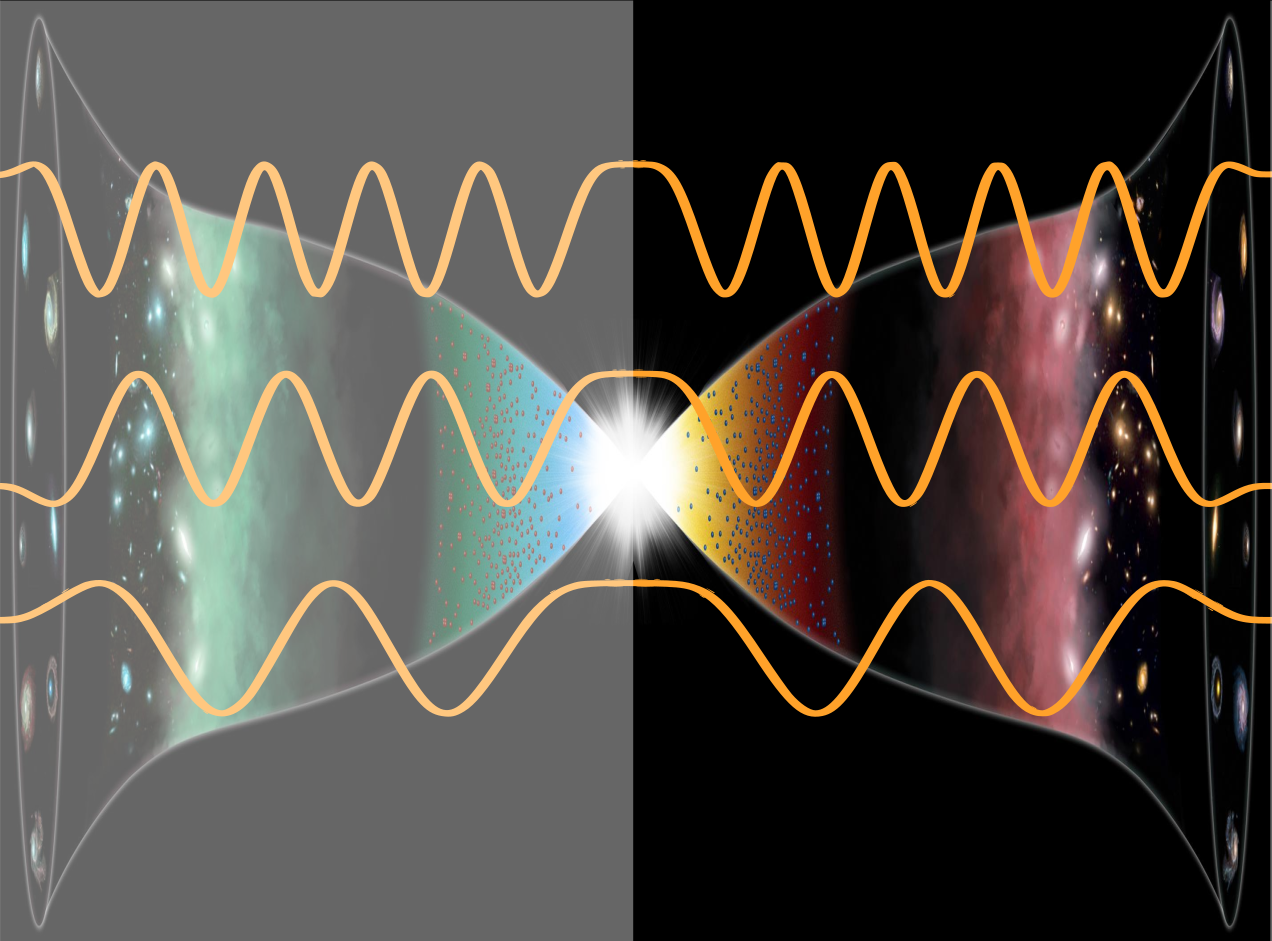
\includegraphics[width=0.6\textwidth]{figures/CPT_periodic.png}
  \end{figure}
  {\large Astrophysics Group, Cavendish Laboratory\\[0.3em]
   University of Cambridge\par}

    \vspace{0.3cm}


  {Queens' College}


  \vspace{1.3cm}

  {\normalsize This dissertation is submitted for the degree of\par}
  \vspace{0.4cm}
  {\large\itshape Doctor of Philosophy in Physics\par}

  \vspace{1.cm}
  {\large September 2026\par}
\end{titlepage}

% ==================== FRONT MATTER ====================
\pagenumbering{roman}
\setcounter{page}{1}

% --- Declaration ---
\chapter*{Declaration}
\addcontentsline{toc}{chapter}{Declaration}

\noindent I hereby declare that this dissertation is the result of my own work and includes nothing which is the outcome of work done in collaboration except as declared in the text and Acknowledgments. It is not substantially the same as any work that has already been submitted for any degree or other qualification. This dissertation does not exceed the prescribed word limit of the Degree Committee.

\vspace{2.5cm}
\noindent\textit{Wei-Ning Deng}\\[0.3em]
\textit{Cambridge, September 2026}

% --- Abstract ---
\chapter*{Abstract}
\addcontentsline{toc}{chapter}{Abstract}

The $CPT$-symmetric universe model of Boyle and Turok posits that the Big Bang acts as a $CPT$-mirror joining our universe to a $CPT$-reversed ``anti-universe'' at the initial singularity. This single global boundary condition has been shown to address several outstanding problems in cosmology and particle physics simultaneously, including the cosmological constant problem, identity of dark matter, flatness and homogeneity, and the scale invariance of the primordial power spectrum, etc, without introducing particle content beyond three right-handed neutrinos, 36 dimension-zero scalar fields, and composite Higgs. The overview of the model is introduced in \cref{chapter:introduction}. 

This thesis investigates two questions left open by this framework: how the requirement of global $CPT$-symmetry constrains the evolution of cosmological perturbations, and whether this macroscopic boundary condition can be justified from a more fundamental, quantum-field-theoretic description of fermions.

Part~I addresses the first question by extending previous work on periodic, spatially flat universes to the spatially curved case. In \cref{chapter:theory} we show that the temporal boundary condition imposed by the future conformal boundary is generically incompatible with the spatial boundary condition required by a closed universe, and that consistency between the two is only possible for a discrete, quantized set of spatial curvatures, which remain consistent with \texttt{Planck 2018} constraints. In \cref{chapter:Observation}, the coupled Einstein--Boltzmann perturbation equations are solved numerically, including radiation anisotropy and higher-order moments, we demonstrate that imposing both boundary conditions simultaneously constrains not just the curvature but the full set of cosmological parameters governing the conformal age of the universe. In \cref{chapter:low-k}, we then relax the high-$k$ approximation used in this analysis and construct mode-mixed solutions that satisfy both boundary conditions at low wavenumber, uncovering distinct suppression and oscillatory features in the CMB power spectra. In \cref{chapter:conclusion_matter_evol}, the conclusion and future work are presented. Finally, we examine the assumptions underlying the matter density near the Big Bang and future conformal boundary, arguing that a classical treatment breaks down in these regimes and motivating a quantum field theoretic description of matter in curved spacetime. Since matter is formed by fermions, this naturally leads to the second question.

Part~II addresses the second question by developing a formalism for fermions based on the K\"{a}hler-Dirac (KD) equation, which is naturally defined on curved spacetime using differential forms (\cref{chapter:Intro_Basics}). We show that the additional $\gamma^0$ required to construct a Lorentz-invariant KD Lagrangian introduces negative-norm and negative-energy states. In \cref{chapter:two-sheet_KD_Majorana}, we resolve this pathology by proposing a two-sheeted, $PT$-reversed spacetime geometry on which these ghost states are reinterpreted as ordinary, positive-energy fermions on a second sheet. Imposing a KD-Majorana condition relating the two sheets ensures that the fields on the second sheet are the exact $CPT$-conjugate antiparticles of those on the first, providing a microscopic justification for global $CPT$-symmetry. In \cref{chapter:SM_Cosmology}, we then show that all sixteen Standard Model fermions (in one generation), including right-handed neutrinos, can be accommodated within exactly four copies of the KD-Majorana field, with the Standard Model gauge group emerging from the symmetries relating these copies and internal symmetry of KD field. The corresponding KD kinetic, Yukawa, and Majorana mass terms are also constructed. As for cosmology, its implication to $CPT$-symmetric universe model is discussed, including its application to Balck hole mirror model. In \cref{chapter:Lag_Euclidean}, we further develop a Euclidean KD Lagrangian that avoids the non-Hermiticity and chiral anomaly present in the standard Euclidean Dirac formulation. Finally, in \cref{chapter:FutureWork_KD}, we outline prospects for extending this two-sheeted KD framework to lattice gauge theory, twistor theory, and string theory.

% --- Acknowledgments ---
\chapter*{Acknowledgments}
\addcontentsline{toc}{chapter}{Acknowledgments}

\begin{CJK}{UTF8}{bsmi}

Completing a PhD is no small task, and I am deeply grateful to everyone who helped me along the way.

In Taiwan, most high school students are encouraged to pursue a practical career, such as medical doctor or lawyer, so I owe a particular debt to the teachers who instead nurtured my interest in science and encouraged me to follow my own path. I am especially grateful to Wan-Ling Chung (鍾菀菱), who supported me in attending the Earth Science Olympiad, where I first discovered my interest in astronomy and cosmology. When I later struggled to choose between becoming a medical doctor and a scientist, Jing-Ting Xu (許靜婷) encouraged me to follow my dream. I still remember her telling me that ``even if the theory you work on turn out to be wrong, it is still precious for expanding human knowledge.'' I also want to thank my physics teacher Jing-Hua Lee (李京華), who helped me prepare for the university entrance examination and taught me to be humble in physics: even when a calculation gives the right answer, that does not mean one truly understands the physical meaning behind it, and that meaning is often far more profound than it first appears.

I am grateful to all the teachers in the Department of Physics at National Taiwan University, especially Yeong-Chuan Kao (高涌泉), in whose course I learned that asking good questions matters more than solving problems for a good physicist. I would also like to thank Hiroyuki Hirashita, Pisin Chen (陳丕燊), and Hsi-Yu Schive (薛熙于) for supervising my undergraduate and master's research. I am especially grateful to Eugene Lim at King's College London, who supervised my summer research project, inspired my love of theoretical physics, and whose project ultimately became my master's thesis; without his help, I could not have applied for a PhD at the University of Cambridge.

Since arriving in Cambridge, I have benefited enormously from its academic environment, particularly the Kavli Institute for Cosmology and the Institute of Astronomy, which host lots of seminars and activities offering opportunities to interact with excellent researchers from around the world. I also want to thank Queens' college, which provide such a warm environment for us to know people working in different research areas. 

Above all, I want to thank my supervisor, Will Handley. When he learned that I was more drawn to theoretical work than to data analysis and model comparison, he pointed me towards the theoretical project that became Part~I of this thesis. I have been continually amazed by how versatile he is: although he specializes in Bayesian analysis, his knowledge is broad enough to span theoretical, observational, and even instrumental work. Because he understands how different people think, he is able to recognize what each of us needs and to work with us accordingly, and this is exactly how he worked with me. Over the course of the project, he taught me the entire process of building a theoretical model and comparing it with observation, training that has been invaluable to me as a cosmologist. He also encouraged me to work alongside AI tools, which greatly accelerated my research and placed me at the forefront of this new era of research, something I am truly grateful for. Moreover, once he learned of my interest in the $CPT$-symmetric universe model, he helped me reach out to Latham Boyle and Neil Turok, the originators of the theory, opening the door to my collaboration with Latham Boyle.

Together with Latham, I worked on an entirely theoretical project in particle physics and theoretical cosmology, which became Part~II of this thesis. He taught me how to think as a theorist. I am continually amazed by how he thinks outside the box, connecting theories that at first seem far apart from one another and revealing relationships between them that are profound rather than merely superficial. I believe the secret lies in his genuine interest in many different theories, pursued without the arrogance sometimes found among theorists, and in the time he devotes to understanding those theories thoroughly. That is precisely what allows him to identify a loophole in one area and to find its resolution in a seemingly unrelated field. I deeply respect this way of thinking and hope to learn from it throughout my own career.

Thanks to my parents, for their continuing love and support, be it financial, emotional, or moral. Last, and most of all, I want to thank my husband, Shih-Huan Huang. We have been classmates since our undergraduate years, applied to Cambridge together, and were both fortunate enough to be awarded scholarships for our PhDs there. Although we work in different fields of physics, I still treasure our discussions after dinner. We had a baby during our second year of the PhD, and he has been a truly wonderful husband and father. Without him, I could not have completed this PhD alongside raising our child.

Finally, I want to thank the Cambridge Trusts Taiwanese Scholarship for their generous financial support, which made this PhD possible.

\end{CJK}

% WND was supported by a Cambridge Trusts Taiwanese Scholarship. WJH was supported by a Royal Society University Research Fellowship. This work was performed using the Cambridge Service for Data Driven Discovery (CSD3), part of which is operated by the University of Cambridge Research Computing on behalf of the STFC DiRAC HPC Facility (www.dirac.ac.uk). The DiRAC component of CSD3 was funded by BEIS capital funding via STFC capital grants ST/P002307/1 and ST/R002452/1 and STFC operations grant ST/R00689X/1. DiRAC is part of the National e-Infrastructure.
% This work was also supported by the UKRI Frontier Research Guarantee [EP/X035344/1] and the UKRI GLITTER grant [EP/Y037332/1].

% --- Tables of Contents & Figures ---
\tableofcontents
\clearpage

\listoffigures
\addcontentsline{toc}{chapter}{List of Figures}
\clearpage

% ==================== MAIN CONTENT ====================
\pagenumbering{arabic}

\chapter{Introduction}\label{chapter:introduction}

% Editor's note: Improved the flow of the opening paragraph. Changed colloquial phrasing to a more formal academic tone.
The $\Lambda$CDM model and the Standard Model successfully explain a wide range of observational and theoretical phenomena in cosmology~\cite{2020A&A...641A...6P} and particle physics~\cite{1995iqft.book.....P}. However, several fundamental issues remain unresolved. In cosmology, these include the horizon~\cite{1972grun.book.....D} and flatness~\cite{1983Natur.305..673C} problems, as well as the unknown composition and nature of dark matter and dark energy. In the Standard Model (SM) of particle physics, outstanding challenges include the cosmological constant problem~\cite{1989RvMP...61....1W}, the Weyl anomaly~\cite{1994CQGra..11.1387D}, and the strong $CP$ problem~\cite{1976PhRvL..37....8T}. Attempts to address these challenges typically involve introducing new degrees of freedom, such as cosmic inflation~\cite{1981PhRvD..23..347G}, novel dark matter particle candidates~\cite{2019Univ....5..213P}, axions~\cite{1977PhRvL..38.1440P}, or modifications to General Relativity~\cite{2012PhR...513....1C}. Despite massive theoretical effort, no single framework has been able to resolve all these issues simultaneously, and such piecemeal additions compromise the apparent simplicity of our universe suggested by recent observations~\cite{2020A&A...641A...6P, 2024ApJ...966..157F}.

To address these challenges comprehensively, \cite{2018PhRvL.121y1301B, 2022AnPhy.43868767B} proposed a novel cosmological model known as the $CPT$-symmetric universe. Rather than introducing ad hoc degrees of freedom, they posited that the universe is strictly $CPT$-symmetric at the Big Bang singularity. Given this single initial condition, many of the aforementioned issues could be solved without adding extraneous theoretical complexity~\cite{2021arXiv211006258B,2022arXiv220810396B,2024PhLB..84938442B,2023arXiv230200344T}.

% Editor's note: Corrected "Big Band" to "Big Bang" and improved sentence structure. Capitalization of "Horizon" was removed.
The foundational inspiration for this model stems from cosmic microwave background (CMB) observations, where primordial perturbations are empirically found to obey Neumann initial conditions ($\partial_t \Phi_k=0$). The conventional explanation for this relies on cosmic inflation: observable modes exited the horizon during the inflationary epoch (freezing out), and as the horizon subsequently grew to encompass these scales again, they began to oscillate, naturally satisfying a Neumann initial condition at horizon reentry. However, if there was no period of cosmic inflation---meaning the universe began at the Big Bang and transitioned directly into a radiation-dominated era---the most straightforward explanation is that the Big Bang itself acts as a temporal mirror. For cosmological perturbations to be differentiable at this initial singularity, they must inherently satisfy Neumann initial conditions (see \cref{fig:CPT_periodic}).

\begin{figure}[htbp]
    \centering
    % Left Subfigure
    \begin{subfigure}[t]{0.48\textwidth}
        \centering
        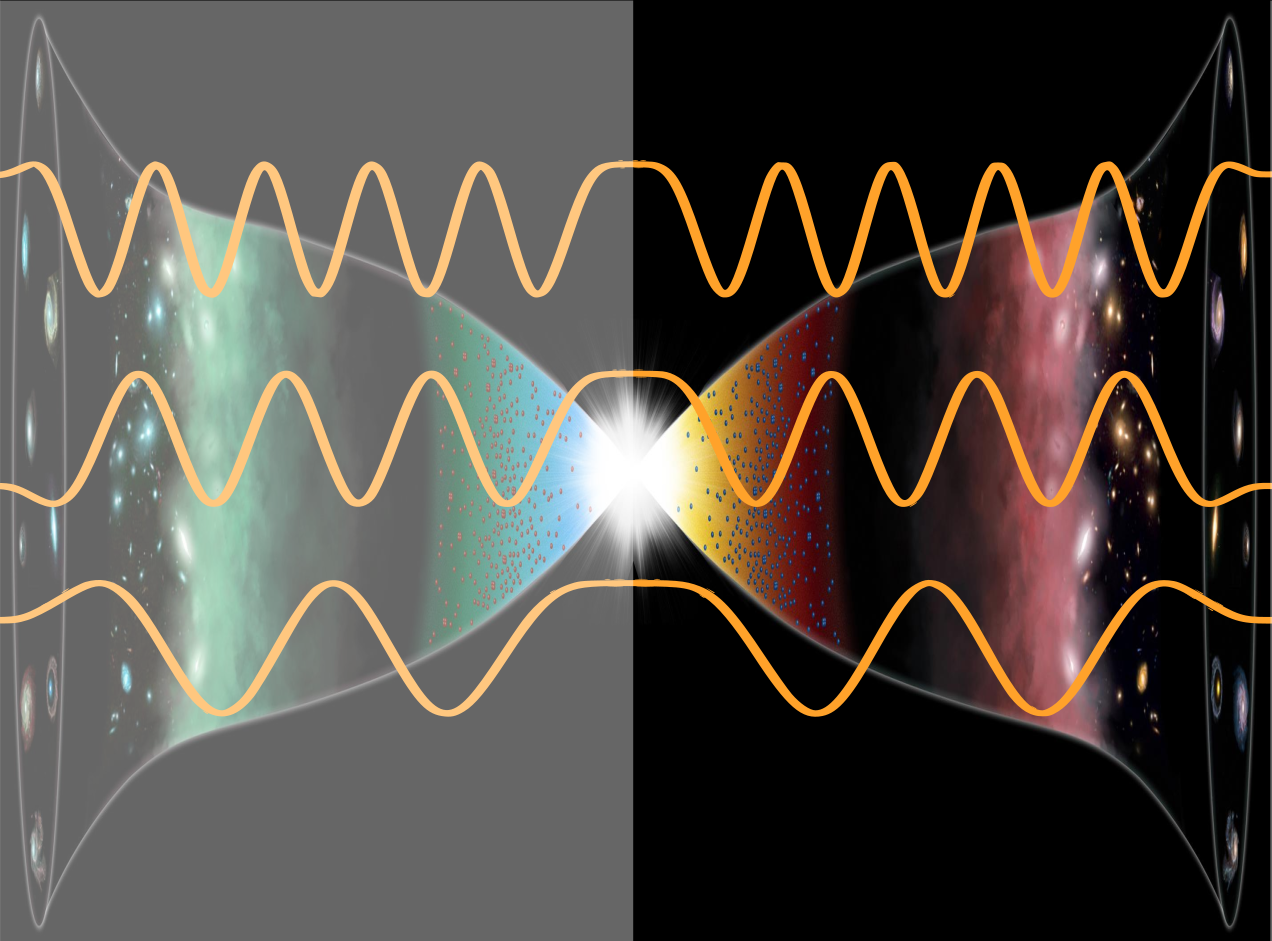
\includegraphics[width=\textwidth]{figures/CPT_periodic.png}
        \caption{Evolution of the scale factor $a$ and perturbations in conformal time. The universe and anti-universe are connected at the Big Bang (a $CPT$-symmetric mirror).}
        \label{fig:CPT_periodic}
    \end{subfigure}%
    \hfill
    % Right Subfigure
    \begin{subfigure}[t]{0.48\textwidth}
        \centering
        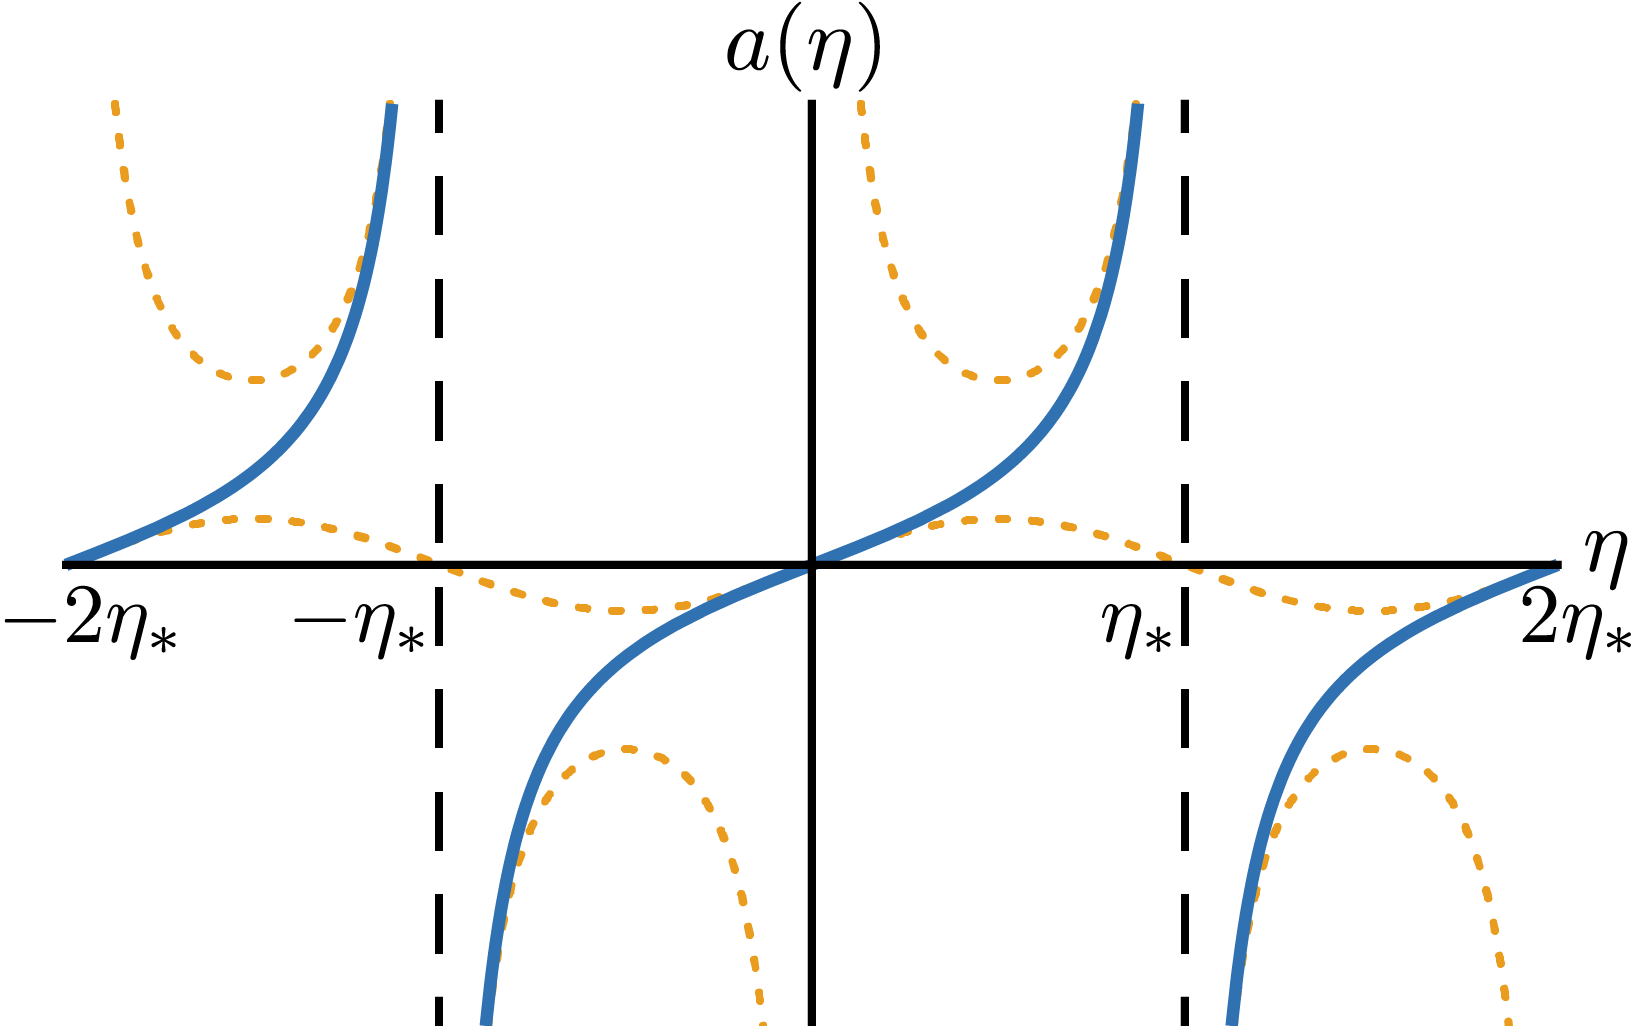
\includegraphics[width=\textwidth]{figures/ScaleFactorFigv2.png}
        \caption{Solution of Friedmann equation in conformal time, which is periodic. The figure is fig.~1 in \protect\cite{2021arXiv210906204B}.}
        \label{fig:a_eta}
    \end{subfigure}

    \caption{Scale factor evolution and periodic behavior in conformal time.}
    \label{fig:a-eta}
\end{figure}

% Editor's note: Fixed grammatical issues regarding spacetime beginning and improved the flow of the transition into QFT.
One might reasonably ask: if spacetime itself begins at the Bang, how can we define ``before'' or ``after'' the universe in a way that allows us to compute derivatives? The solution requires transitioning to conformal time, $d\eta=\frac{dt}{a}$. From the perspective of an observer co-expanding with the universe, the conformal age of the universe is finite, allowing one to mathematically pass through the boundaries of the universe to trace its continuous evolution. Indeed, the solution to the Friedmann equations in conformal time can be expressed as a Jacobi elliptic function~\cite{2021arXiv210906204B, 2024PhLB..84938442B}, which is inherently periodic (\cref{fig:a_eta}). Establishing that the scale factor satisfies this ``mirror'' condition at the Big Bang naturally raises the next question: how do particles and quantum fields behave under this symmetry?

Interestingly, quantum field theory (QFT) possesses a fundamental global symmetry: $CPT$-symmetry, which states that physical laws remain invariant under the simultaneous reversal of charge, parity, and time. For instance, a left-handed electron moving forward in time follows the exact same physical laws as a right-handed positron moving backward in time. While this symmetry is traditionally applied locally, one may hypothesize the existence of a global $CPT$-symmetry. This would imply the existence of an ``anti-universe'' prior to the Big Bang that is exactly $CPT$-symmetric to ours, wherein all physical quantities are $CPT$-reversed but governed by identical physical laws. This conceptual leap led Boyle and Turok to construct the $CPT$-symmetric universe model. Remarkably, they found that numerous problems in both cosmology and the SM could be resolved under this framework without introducing additional complexity. A conceptual map of these solutions is provided in \cref{fig:CPT_solve_problems}, which includes citations to the relevant literature.

\begin{figure}[htbp]
     \centering
     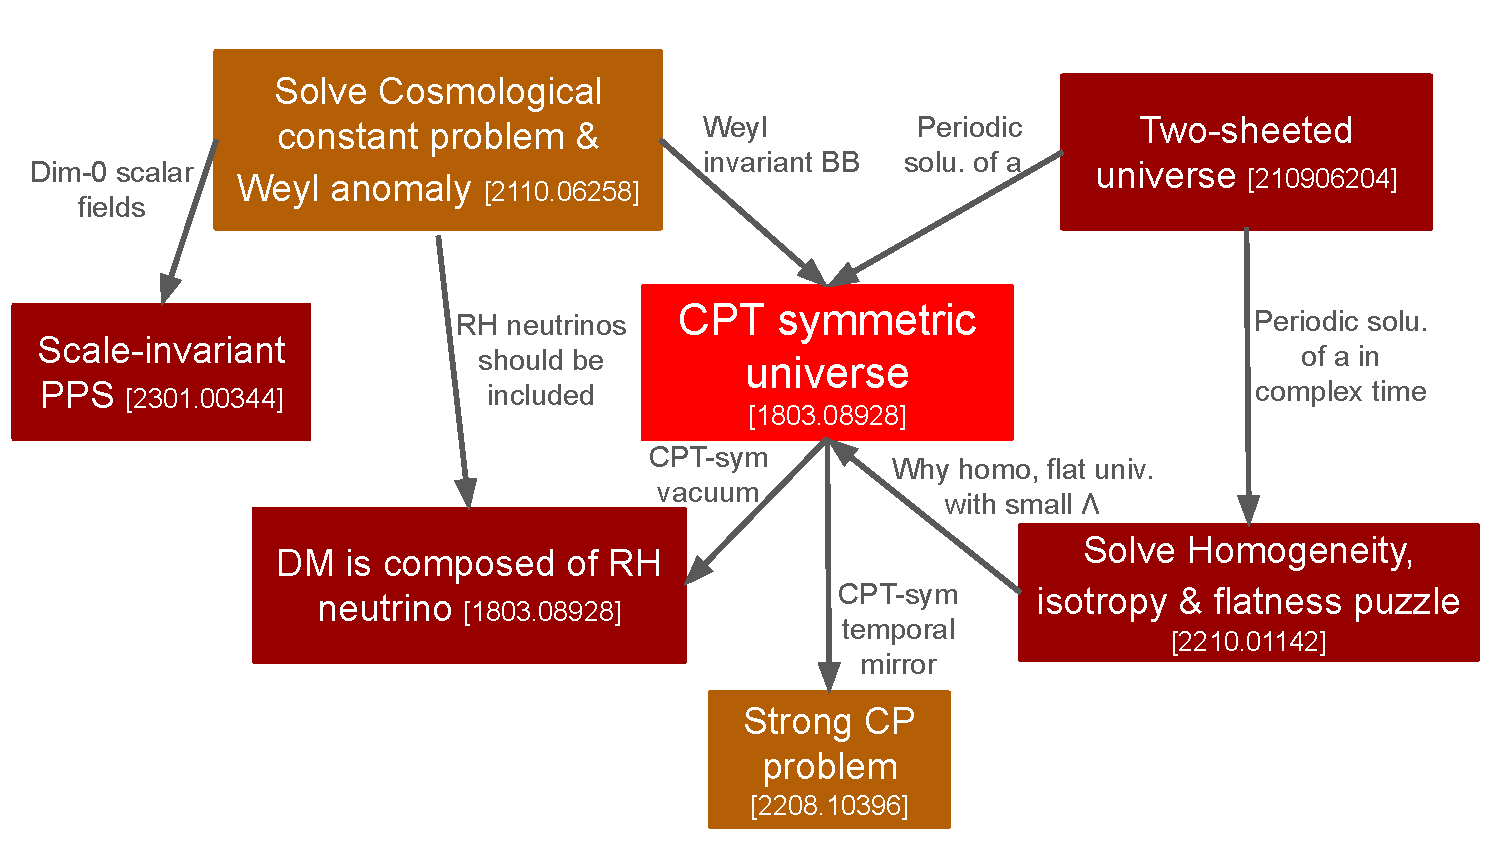
\includegraphics[width=\textwidth]{figures/CPT_univ_solve_problems.pdf}
     \caption{Problems in cosmology (dark red) and the SM particle physics (brown) which could be solved by CPT-symmetric universe. The relationship between the concepts are shown with arrows, and the arXiv number to the related papers is included.}
     \label{fig:CPT_solve_problems}
\end{figure}

% Editor's note: Fixed "seesaw machenism", corrected grammar in the 36 dimension-zero scalars, and tightened sentence structure.
For example, by resolving the cosmological constant problem, the Weyl anomaly, and UV divergences when coupling QFT to gravity, it was shown that given the standard SM gauge group $SU(3)\times SU(2)\times U(1)$ (totaling 12 spin-1 degrees of freedom), consistency requires exactly three generations of fermions (including right-handed neutrinos) and 36 dimension-zero scalar fields, while forcing the Higgs boson to be composite \cite{2021arXiv211006258B, boyle2025fixedpointsclassicalgravity}. In other words, no exotic new particles are strictly required beyond 3 right-handed (RH) neutrinos and the dimension-zero scalar fields (see \cref{fig:SM_particles_dim0_RHnu}). The existence of RH neutrinos is already strongly supported by the observation of neutrino oscillations, which proves that left-handed (LH) neutrinos possess mass. The most natural explanation for this is the introduction of a Majorana mass term for the RH neutrinos. Through interactions with the Higgs boson, this effectively grants mass to the LH neutrinos via the seesaw mechanism, where lighter LH neutrinos naturally correspond to more massive RH neutrinos.

\begin{figure}[htbp]
     \centering
     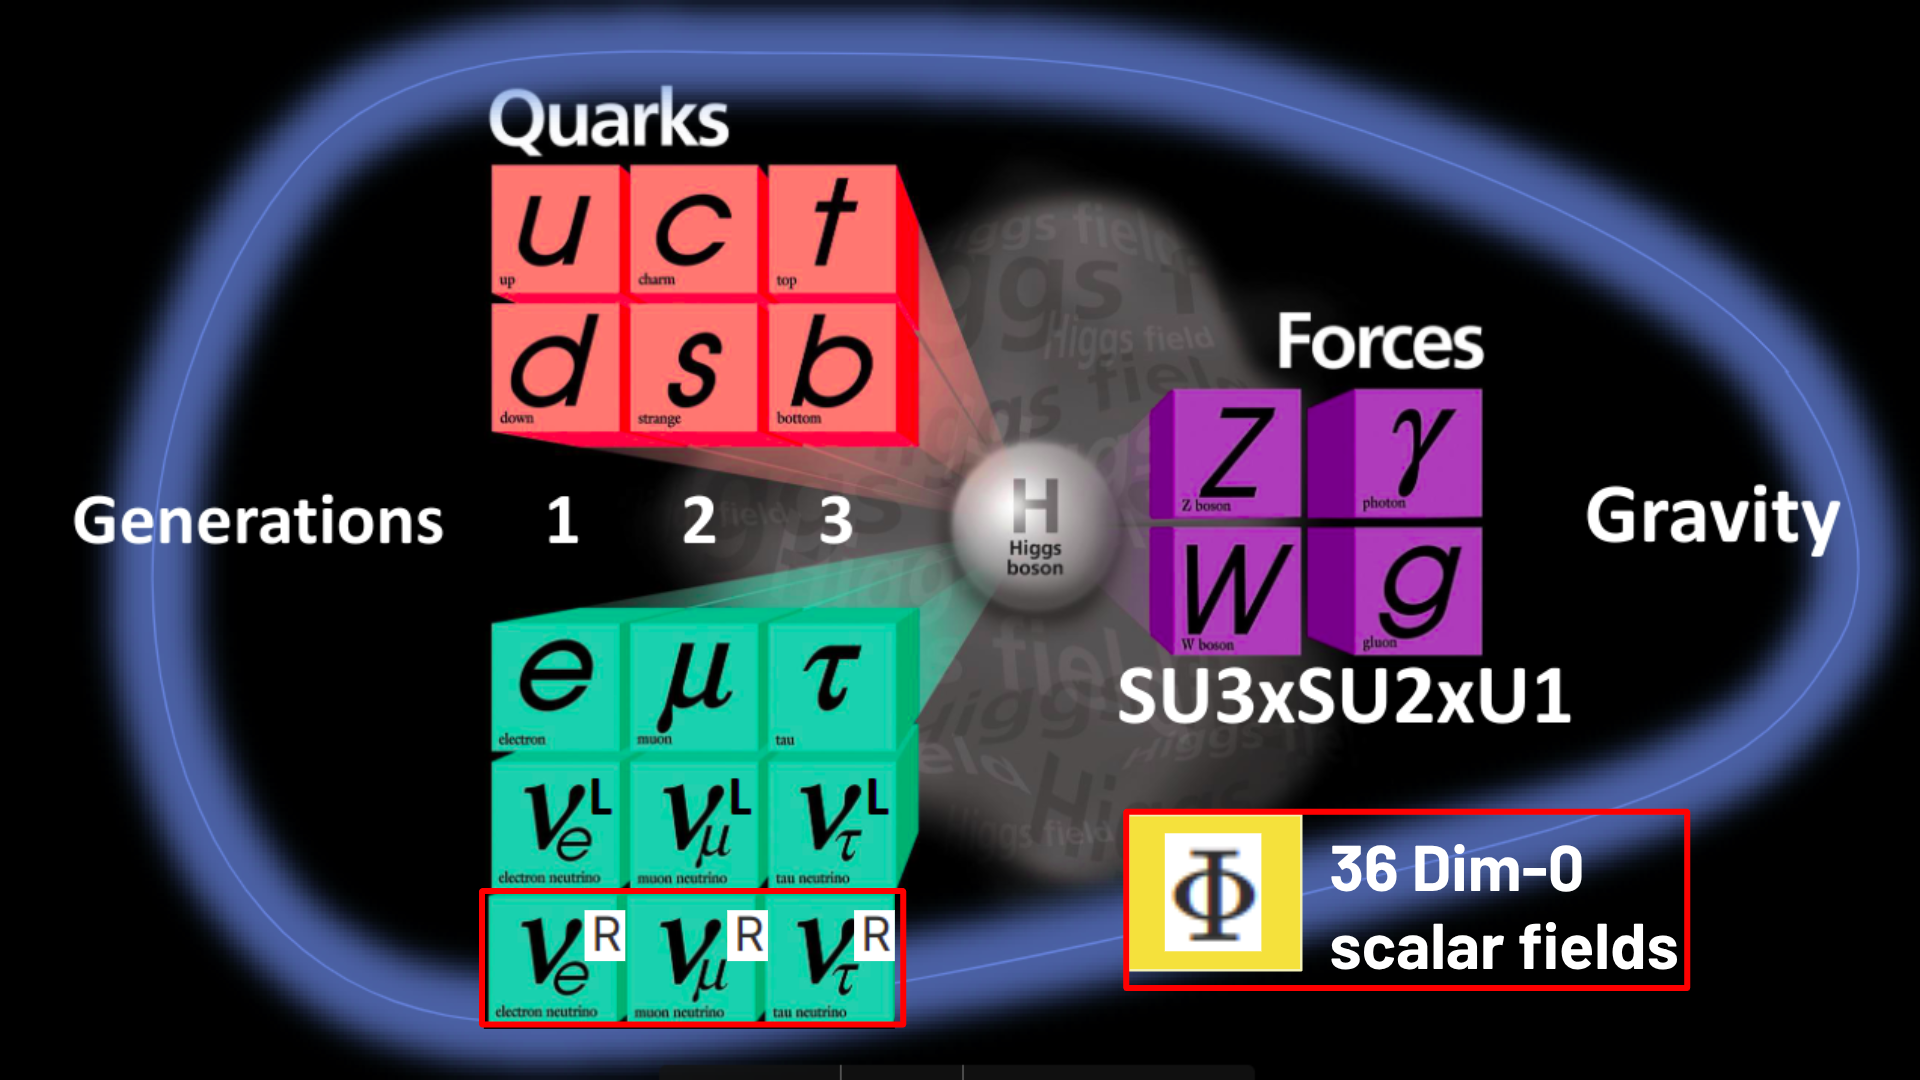
\includegraphics[width=0.75\textwidth]{figures/SM_particles_dim0_RHnu.png}
     \caption{Table for fundamental particles in order to solve cosmological constant problem. 3 right-handed neutrinos and 36 dim-0 scalar field are included, while Higgs boson should be composite.}
     \label{fig:SM_particles_dim0_RHnu}
\end{figure}

% Editor's note: Clarified "HPC" which contextually means "high-energy colliders" rather than high-performance computing. Fixed tense and flow.
Consequently, since this framework limits the addition of new SM particles, dark matter (DM) must be composed of one of these RH neutrinos. Based on neutrino oscillation data, the mass-squared differences between the three neutrino generations are known, but their absolute mass scale remains undetermined. This ambiguity provides the freedom to set the lightest LH neutrino mass to exactly zero. By doing so, the seesaw mechanism is effectively ``switched off'' for one RH-LH neutrino pair, rendering that specific RH neutrino entirely stable. Because it does not interact with the Higgs boson or LH neutrinos, it cannot be produced via standard thermal bath freeze-out. Instead, it is produced through a mechanism analogous to Hawking radiation: particles are spontaneously created from the vacuum in an accelerating frame. Similarly, an observer in the late-time universe would observe particles created directly from the $CPT$-symmetric vacuum at the Big Bang. If we require this specific particle to account for $100\%$ of the observed dark matter density, the required RH neutrino mass is uniquely constrained to $4.8\times 10^8 $ GeV \cite{2018PhRvL.121y1301B, 2022AnPhy.43868767B}. Such an immense mass naturally explains why it has eluded detection at high-energy particle colliders. Furthermore, the requirement that the lightest neutrino is massless implies that the sum of the neutrino masses must sit at the absolute theoretical minimum ($0.06$ eV or $0.1$ eV for normal and inverted hierarchies, respectively). This prediction tightly aligns with ongoing cosmological observations from CMB and BAO surveys \cite{Adame_2025, PhysRevD.111.083535}, which continue to place increasingly stringent upper limits on this mass sum. \footnote{Interestingly, if empirical constraints allow the sum of neutrino masses to be mathematically negative, current data actually favor a slightly negative value. This anomaly might be related to other observational tensions in cosmology, such as larger-than-expected CMB lensing or dynamical dark energy \cite{PhysRevD.111.083507}. However, this remains an unresolved and highly active research topic.}

% Editor's note: Rephrased the baryonic asymmetry explanation to sound more formal, removing casual phrasing like "nature prefer matter then anti-matter".
Regarding the other two RH neutrinos, they provide an elegant mechanism for generating the observed baryon asymmetry. The dominant paradigm for this asymmetry relies on $CP$-violation. However, relying solely on standard SM processes yields a baryon asymmetry several orders of magnitude too small to match observations. By incorporating these two highly massive RH neutrinos, the situation changes: they rapidly decay into Higgs bosons and leptons (or their antiparticles) prior to electroweak symmetry breaking. Due to inherent $CP$-violation, the decay rates for these two channels are asymmetric, generating a net lepton asymmetry. These leptons are subsequently converted into baryons via non-perturbative sphaleron processes (\cite{PhysRevD.30.2212, PhysRevD.36.581}), efficiently transferring the lepton asymmetry into the observed baryon asymmetry. One might philosophically ask why nature seemingly prefers matter over antimatter in the first place. The $CPT$-symmetric universe model beautifully answers this: the pre-Bang ``anti-universe'' inherently contains an equal and opposite excess of antimatter. Across the entire global timeline, the net asymmetry identically cancels out, preserving fundamental balance.

\footnote{While utilizing RH neutrinos is the most straightforward mechanism for explaining baryon asymmetry within the SM, making precise quantitative predictions to compare with data remains exceedingly difficult. Adding RH neutrinos to the SM introduces 10 new degrees of freedom, encompassing the new masses and mixing phases. Low-energy experiments (e.g., neutrino oscillations, neutrinoless double $\beta$ decay) can currently constrain only 4 of these parameters (3 masses and 1 phase). The remaining parameters predominantly govern physics at energy scales far beyond current experimental reach, rendering them difficult to constrain empirically.}

% Editor's note: Corrected "Lymann-$\alpha$" to "Lyman-$\alpha$". Fixed grammar concerning the dimension-zero fields.
Regarding the 36 dimension-zero scalar fields, their dimensionless nature means they possess no preferred physical scale, effectively behaving mathematically like white noise. Consequently, if the initial conditions of primordial perturbations are driven by the quantum fluctuations of these fields, the resulting spectrum is naturally scale-invariant. Strikingly, theoretical predictions for the scalar amplitude $A_s$ and the spectral index $n_s$ derived from this mechanism fall remarkably close to observed values \cite{2023arXiv230200344T}. This offers a completely novel genesis for the primordial power spectrum (PPS) without invoking cosmic inflation. Interestingly, recent observations by ACT, SPT, DESI, and Lyman-$\alpha$ forest surveys suggest a slightly larger value for $n_s$ alongside a non-zero running index $\alpha=dn_s/d\ln k$, placing intense pressure on standard inflationary models (e.g., Starobinsky and Higgs inflation for specific potentials and $e$-folds $N_\star$) \cite{Balkenhol2025, mcdonough2026spectrumnsconstraintsdesi, pwfl-mt4g}. When combined with stringent upper bounds on the tensor-to-scalar ratio $r$ \cite{PhysRevD.105.083524} (where the dimension-zero mechanism strictly predicts $r=0$), observational evidence may ultimately favor this non-inflationary PPS genesis.

What, then, is the role of the Higgs boson? One hypothesis suggests that the Higgs is a composite state constructed from the 36 dimension-zero scalars. Following methodologies analogous to string theory, one can theoretically construct dimension-1 fields (such as the Higgs) from fundamental dimension-0 fields. Such a composite Higgs model possesses the potential to resolve the hierarchy problem: the exponential decay of the coupling constant could naturally explain why the electroweak scale (and consequently the Higgs mass) is vastly suppressed relative to the Planck scale. Nevertheless, this framework remains heavily under exploration and faces significant theoretical hurdles: (1) explaining how dimension-0 fields dynamically emerge from gravity, (2) the current inability to robustly form a standard Higgs doublet, and (3) the presence of non-unitary and non-Hermitian states (ghosts) arising from the four-derivative kinetic terms. \footnote{There are two potential pathways to eliminate these ghosts. First, as demonstrated by \citet{Bender:2007wu} and \cite{PhysRevD.97.045001}, fourth-order derivative $\mathcal{PT}$-symmetric theories are not inherently doomed by negative-norm ghosts. If one abandons the standard Dirac-Hermitian inner product and instead evaluates the $\mathcal{PT}$-symmetric Hamiltonian using a $\mathcal{PT}$ or $\mathcal{V}$ inner product, the energy spectrum remains strictly real and the Hilbert space maintains a positive-definite norm. Second, if the ghost is of the Ostrogradskian type---signifying a classical instability driven by higher-derivative terms---it might be resolved by strictly constraining the permissible classical trajectories \cite{Chen:2012au}.}

These theoretical challenges point toward an alternative avenue for generating a scale-invariant PPS without inflation: quadratic gravity \cite{PhysRevD.97.126005}. Because it incorporates four derivatives, quadratic gravity serves as a UV-complete theory of quantum gravity. The four-derivative Lagrangian can generate a scale-invariant PPS via a mechanism conceptually similar to the dimension-zero scalar field; crucially, however, the PPS is generated directly by the quantum fluctuations of spacetime itself rather than an external matter field. This paradigm is highly attractive as it simultaneously provides a theory of quantum gravity and explains the scale-invariant PPS without discarding a fundamental Higgs boson. However, substantial theoretical development is still required to formalize this hypothesis.

% Editor's note: Fixed "horizen", "then", and smoothed the explanation of standard inflationary solutions vs the CPT-symmetric thermodynamic solution.
Finally, we must address the cosmological flatness and horizon problems. Cosmic inflation solves these by positing an era of exponential expansion, stretching the universe such that our observable patch is vastly smaller than the global volume. This inherently flattens local curvature and ensures that the entire observable universe was previously in causal, thermal contact.

In stark contrast, the $CPT$-symmetric universe model resolves these issues using a completely different framework: thermodynamics. Because the scale factor solution is periodic in both real and imaginary conformal time, one can compute the gravitational entropy of the universe by integrating over one full period in imaginary time, directly mirroring the technique pioneered by Hawking and Gibbons for black hole thermodynamics~\cite{1977PhRvD..15.2752G}. Remarkably, this calculation reveals that the cosmological state possessing the maximum entropy---and thus the highest statistical probability---is one that is strictly homogeneous, isotropic, and flat \cite{2024PhLB..84938442B}.

\begin{figure}[htbp]
     \centering
     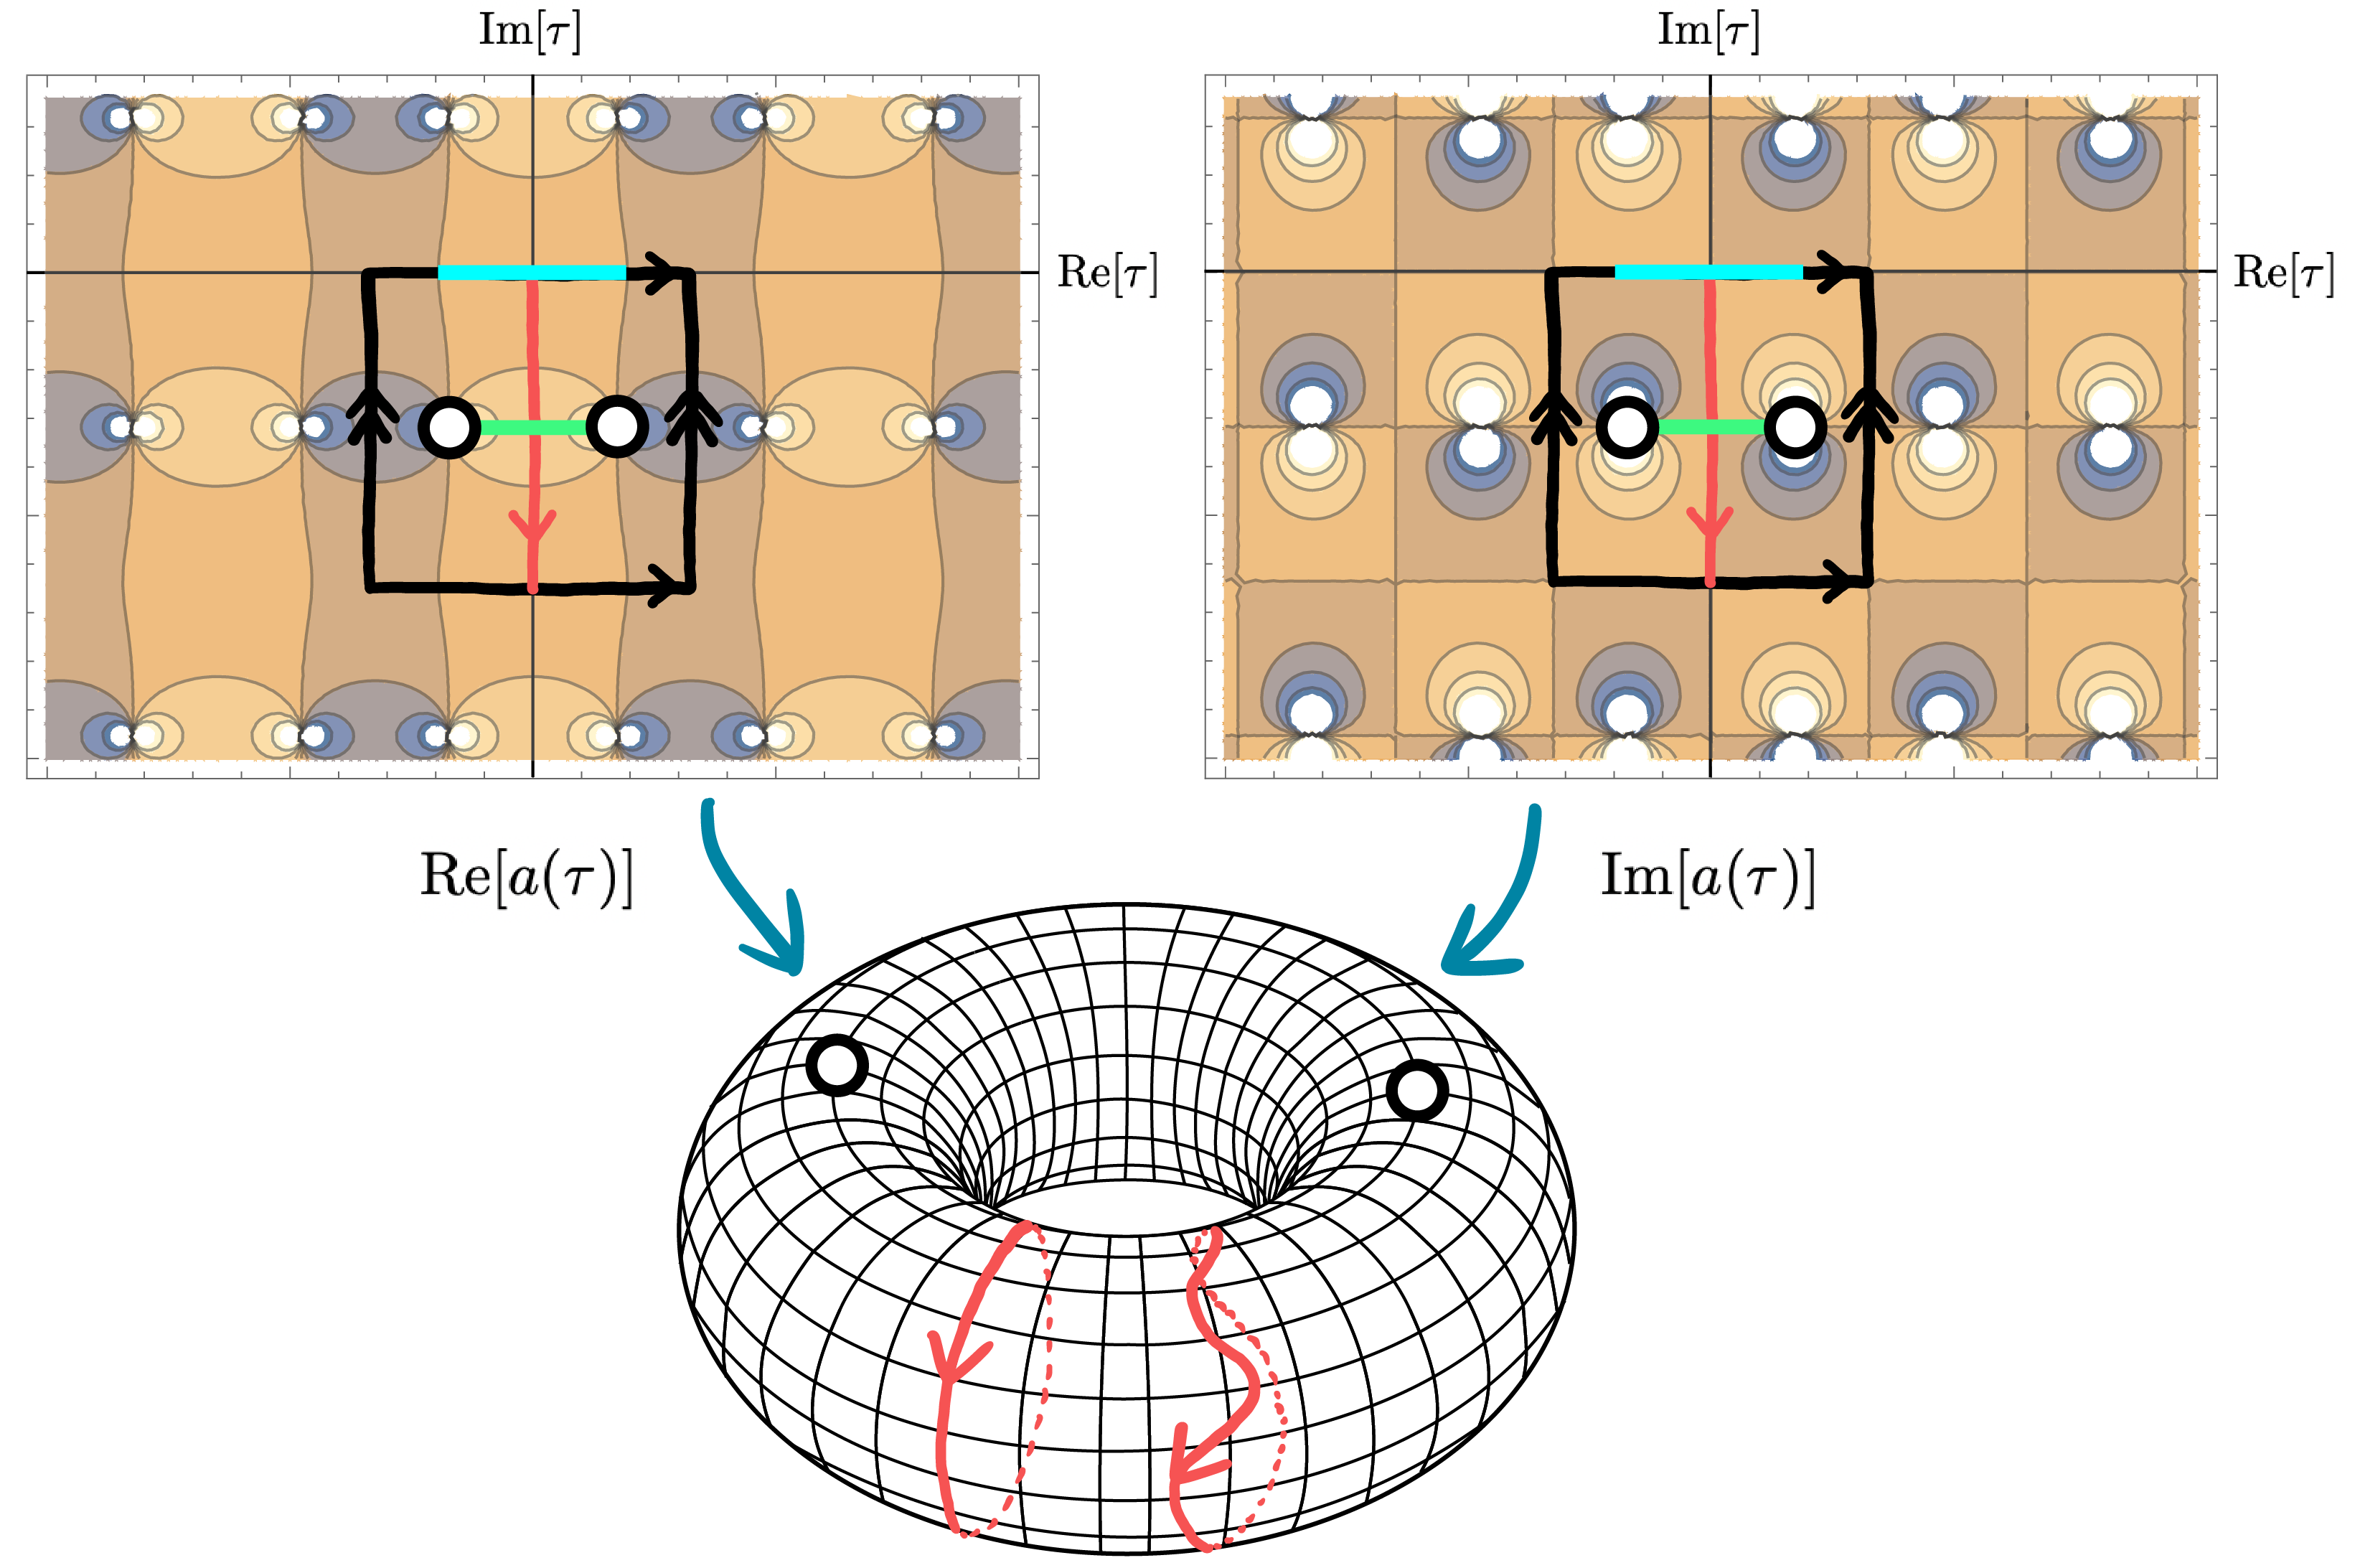
\includegraphics[width=0.6\textwidth]{figures/TorusFig2.png}
     \caption{Solution of scale factor in complex conformal time plane, and how they integrate through one conformal time to calculate gravitational entropy. This figure is fig.~1 in \cite{2024PhLB..84938442B}.}
     \label{fig:a_Torus}
\end{figure}

Thus far, we have outlined how the $CPT$-symmetric universe elegantly resolves multiple longstanding crises in both cosmology and the SM. However, critical questions remain. First, how do cosmological perturbations evolve within such a universe, and do these global symmetry conditions impose novel constraints on the standard cosmological parameters? Second, while global $CPT$-symmetry is a powerful phenomenological tool for describing the macroscopic universe, is there a rigorous theoretical justification at the quantum scale demanding that this boundary condition be satisfied?

Answering these two fundamental questions is the primary objective of this thesis, which is structured into Part~I and Part~II, respectively.

In Part~I, we explore the precise impact of a globally periodic structure on cosmological perturbations. Lasenby and Handley previously investigated this dynamic within the context of spatially flat universes \cite{Lasenby_2022}. Their work demonstrated that temporal periodic conditions impose strict boundary constraints on perturbations, leading to observable effects in the CMB power spectrum \cite{Bartlett_2022,Prathaban_2022}. In \cref{chapter:theory}, I extend this investigation to spatially curved universes. Our analysis reveals that the temporal boundary constraints imposed by the end of the universe (Future Conformal Boundary, FCB) inherently conflict with the spatial boundary conditions demanded by a closed universe. To mathematically resolve this conflict, only a discrete set of specific spatial curvatures is permissible. Remarkably, we demonstrate that these strictly quantized curvature values remain consistent with current observational limits from the \texttt{Planck 2018} data release \cite{Planck2018}. The detailed methodology and implications of this discovery are based on our published work \cite{PhysRevD.110.103528}.

% Editor's note: Improved flow and corrected grammatical issues ("our another"). Inserted "In Chapter 3" to logically organize the paragraph structure.
In \cref{chapter:Observation}, we extend this framework to a realistic cosmological model by solving the coupled perturbations numerically, explicitly incorporating radiation anisotropy and higher-order Boltzmann moments. By simultaneously matching both the temporal and spatial boundary conditions (BCs), we demonstrate that not only the spatial curvature, but all cosmological parameters dictating the conformal age of the universe are constrained. This chapter is based on another of our published works \cite{pjz6-47jv}. Up to this point, our analysis relied on a high-$k$ approximation, where discrete wave vectors are assumed to be equally spaced. This approximation, however, breaks down in the low-$k$ regime. Consequently, in \cref{chapter:low-k}, we construct specific linear combination states to find a general solution that rigorously satisfies both spatial and temporal BCs at low frequencies. The resulting mode mixing and mode omissions introduce distinct suppression and oscillation features in the primordial and CMB power spectra; these findings form the basis of an upcoming publication. Finally, in \cref{chapter:conclusion_matter_evol}, we discuss the hidden symmetry assumptions regarding the matter density at the Big Bang and the future conformal boundary (FCB). One theoretical paradigm suggests that near these two extreme eras, classical approximations inevitably break down, necessitating a full quantum field theoretic treatment. Because matter is fundamentally composed of fermions, tracking its evolution requires solving the Dirac equation in highly curved spacetime, naturally leading us into the second part of this thesis.

% Editor's note: Fixed "property" -> "properties", "normal" -> "standard". Changed "which could be ignored" to "which cannot be ignored" as curvature is extreme at the Bang (please verify this intent!). Fixed "Lorentzian" -> "Lorentz-invariant".
In Part~II, we investigate the fundamental properties of fermions within the $CPT$-symmetric framework. Instead of the standard Dirac equation, the K\"{a}hler-Dirac (KD) equation is utilized. Because it is constructed using differential forms, the KD equation is naturally accommodated in curved spacetime---a feature that cannot be ignored near the singularities of the Big Bang and the FCB. In \cref{chapter:Intro_Basics}, the mathematical basics of KD fermions are introduced. Because the KD field is effectively a $4\times 4$ spinor matrix, an additional $\gamma^0$ matrix must be incorporated to formulate a Lorentz-invariant Lagrangian. However, this additional $\gamma^0$ dictates that half of the field components inherently exhibit negative norms or negative energies (ghosts). To resolve this problem, in \cref{chapter:two-sheet_KD_Majorana}, we propose a two-sheeted, $PT$-reversed spacetime geometry, where the negative-norm states exclusively reside on the second sheet. Due to this $PT$-reversal, these states physically manifest with negative energies to observers in the first sheet. To preserve physical consistency under charge conjugation, a KD-Majorana condition is applied, mathematically constraining the fermions on the second sheet to act as the exact anti-fermions of the first sheet. This elegantly explains why strict $CPT$-symmetry is conserved even at the quantum scale.

% Editor's note: Smoothed the integration of the SM, fixed subject-verb agreements (e.g., "group emerge" -> "group emerges"), and corrected typographical errors like "BHs acting".
In \cref{chapter:SM_Cosmology}, we apply this KD formalism directly to the Standard Model (SM) and cosmology. All 16 fundamental fermions (including the right-handed neutrinos) are elegantly accommodated into exactly four copies of the KD-Majorana field. We demonstrate how the SM gauge group naturally emerges from the transformations between these four copies and the internal symmetries of the KD algebra. Furthermore, the KD formulation of fermion kinetic terms, Yukawa couplings, and right-handed Majorana mass terms are provided. We also discuss the broader implications of this model for the $CPT$-symmetric universe, specifically exploring its application to Black Hole (BH) mirrors \cite{tzanavaris2025blackmirrorscptsymmetricalternatives}---a theory proposing that black holes act as localized $CPT$-symmetric mirrors bridging our universe and the anti-universe. In \cref{chapter:Lag_Euclidean}, we explore the Euclidean Lagrangian for KD fermions, which offers a potential resolution to the non-Hermitian and chiral anomalies inherent in the standard Euclidean Dirac Lagrangian. The properties of other possible KD Lagrangian formulations are also evaluated. Finally, \cref{chapter:FutureWork_KD} outlines compelling directions for future research, including the application of this framework to lattice gauge theory, twistor theory, and potentially superstring theory. Ultimately, framing KD fermions within this two-sheeted topological geometry appears to offer novel solutions to many longstanding problems in theoretical physics.

\printbibliography[heading=subbibliography,title={References}]

% ==================== PART I ====================
\part{Cosmological Constraints from Perturbations in a Periodic Universe} \label{part:constraint_perturb}


\chapter{Predicting spatial curvature $\Omega_K$ in globally $CPT$-symmetric universes}\label{chapter:theory} % Force line breaks with \\

\chapterabstract{
    Boyle and Turok's $CPT$-symmetric universe model posits that the universe was symmetric at the Big Bang, addressing numerous problems in both cosmology and the Standard Model of particle physics. We extend this model by incorporating the symmetric conditions at the end of the Universe, which impose constraints on the allowed perturbation modes. These constrained modes conflict with the integer wave vectors required by the global spatial geometry in a closed universe. To resolve this conflict, only specific values of curvature are permissible, and in particular the curvature density is constrained to be $\Omega_K \in \{-0.016, -0.011, -0.004, \ldots\}$, consistent with \textit{Planck} observations.
}


\section{Introduction}

In this chapter, we investigate the impact of this periodic global structure on cosmological perturbations. Previous work by \citet{2022PhRvD.105h3514L} has explored this concept within the context of flat universes. They found that the physical solutions should not just symmetric at the Bang (satisfying Neumann IC), but also be symmetric or anti-symmetric at the future conformal boundary. The periodic conditions constrain the allowed wave vectors for perturbations to be some discrete values, which have observable effects on the Cosmic Microwave Background (CMB) power spectrum~\cite{2022PhRvD.105h3515B,2022PhRvD.105l3508P}.

Building on this work, we extend the analysis of \citet{2022PhRvD.105h3514L} to include curved universes. Our findings indicate that the discrete wave vectors imposed by the future conformal boundary conflict with the one from spatial boundary conditions in a closed universe. To reconcile this conflict, only specific values of curvature are permissible, which are consistent with the observations from \texttt{Planck 2018}~\cite{2020A&A...641A...6P}. 

\section{Background and perturbations} 
We build on the derivation presented in \citet{2022PhRvD.105h3514L} and extend it to a curved universe. The perturbed FLRW metric can be written as:
\begin{equation}
    ds^2 = a^2 \left[-(1 + 2\Phi)d\eta^2 + (1 - 2\Phi)\left(\frac{1}{1-\kappa r^2}dr^2+r^2d\Omega^2\right) \right],
\end{equation}
where \(\Phi\) is the perturbation in the Newtonian gauge, and $\kappa$ controls the spatial curvature of the universe.

We analyse the evolution of the background in conformal time \(\eta\) instead of physical time to render explicit the periodic behaviour of the universe. Following Lasenby~\cite{2022PhRvD.105h3514L}, only three components are considered: dark energy $\lambda$, radiation $r$, and spatial curvature $\kappa$, omitting matter. The zero-order Friedmann equations are: 
\begin{equation}\label{eq:friedmann_eq_theory}
    \dot{a}^2 = \tfrac{1}{3}\lambda a^4 - \kappa a^2  + \tfrac{1}{3} r, \qquad 
    \ddot{a} = \tfrac{2}{3}\lambda a^3 - \kappa a,
\end{equation}
where \(\hbar = c = 8\pi G = 1\) and dots denote \(d/d\eta\).

The solution to \cref{eq:friedmann_eq_theory} can be expressed as a Jacobi elliptic function~\cite{2021arXiv210906204B}, which exhibits periodic global structure in conformal time. The universe begins at the Big Bang \(a = 0\), evolves to the end of the universe at \(a=\infty\) at a finite conformal time \(\eta_{\infty}\) termed the future conformal boundary (FCB), and then returns from the future boundary back to a future Big Bang, starting the cycle over again. However, this cyclic behaviour does not by default hold for perturbations. To maintain the behaviour, the perturbations should be symmetric not just at the Bang, but also at the FCB. The symmetry constrains the allowed modes of perturbations (see \cref{fig:a_perturbations-eta}).
\begin{figure*}[!ht]\centering
     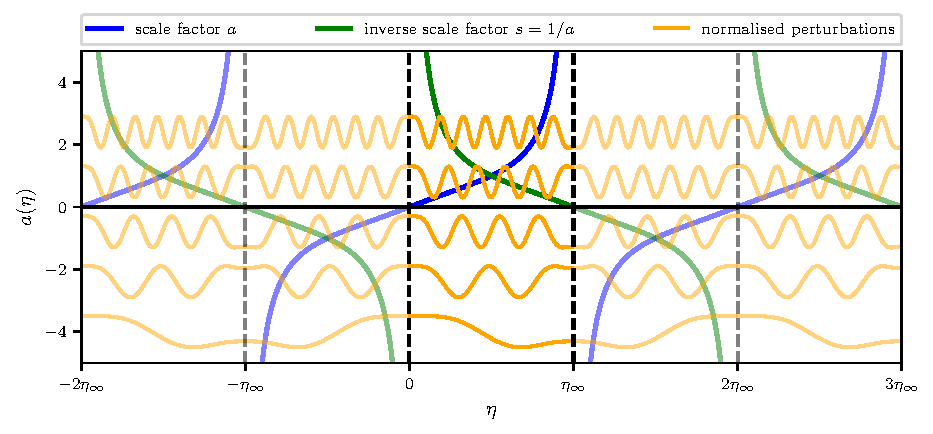
\includegraphics{./parts/part1/figures/a_perturbations-eta.pdf}
     \caption{Evolution of the scale factor \(a\), its reciprocal \(s\equiv 1/a\), and the first five allowed perturbations which are (anti)-symmetric about the future conformal boundary. The perturbations have been normalised to have constant oscillatory amplitude across cosmic time for clarity.}
     \label{fig:a_perturbations-eta}
\end{figure*}

To analyse the perturbations, we write the first-order Einstein equation as:
\begin{equation}\label{eq:perturbation_eq}
    \ddot{\Phi} + 4aH\dot{\Phi} + \tfrac{1}{3}(k^2 + 4a^2\lambda-12\kappa)\Phi = 0.
\end{equation}
where \(k\) is the comoving wave vector of the perturbation. Switching the independent variable from conformal time $\eta$ to scale factor $a$, one finds
\begin{equation}\label{eq:perturbation_a}
    (\lambda a^2 - 3\kappa + \frac{r}{a^2} )\Phi'' + (6\lambda a - \frac{15\kappa}{a} + \frac{4r}{a^3})\Phi' + (4\lambda+\frac{k^2-12\kappa}{a^2})\Phi = 0,
\end{equation}
where a prime denotes \(d/da\).

One degree of freedom between \(r\) and \(\lambda\) can be removed from \cref{eq:friedmann_eq_theory,eq:perturbation_a} by fixing the scaling of \(a\). Following~\cite{2022PhRvD.105h3514L}, \(r = \lambda\) is chosen, equivalent to demanding \(a=1\) when the energy density of matter radiation and dark energy are equal, after which \cref{eq:perturbation_a} becomes
\begin{equation}\label{eq:Phi_ODE}
    a(a^4 - 2a^2 \tilde\kappa + 1) \Phi'' + (6a^4- 10a^2 \tilde\kappa + 4 ) \Phi' + a(4a^2 + \tilde{k}^2-8\tilde\kappa) \Phi = 0, 
\end{equation}
\vspace{-2.5em}
\[ \text{where} \qquad
    \tilde{k} \equiv k/\sqrt{\lambda}, \qquad \tilde \kappa \equiv \frac{3}{2\lambda}\kappa\]
are the dimensionless wave vector and curvature respectively. The factor $\frac{3}{2}$ in $\tilde\kappa\equiv \frac{3}{2\lambda}\kappa$ is chosen such that $\tilde\kappa=1$ corresponds to the transition between a turnaround and a de-Sitter universe, which will be explained later. This equation reduces to eq.~(23) in~\citet{2022PhRvD.105h3514L} when \( \tilde\kappa = 0 \).
Note that if we replace \(\Phi(a)\) with \(\varphi(a) \equiv a^2 \Phi(a)\), the equation remains invariant under the transformation \({a\leftrightarrow1/a}\). This symmetry is important in the next section when considering perturbations passing through the FCB as \(a\rightarrow \infty\).

This equation can be solved analytically, yielding two solutions, both expressed in terms of Heun functions. Observing the CMB power spectrum told us that the solution must satisfy the Neumann initial conditions \(\Phi(a = 0) = C\) and \(\Phi'(a = 0) = 0\), where \(C\) is a constant \footnote{The conventional explanation is from cosmic inflation: the perturbation remains frozen at the beginning and starts oscillating after crossing the horizon \((k = aH)\); on the other hand, in CPT-symmetric universe model, the perturbation solutions should be symmetric at the Big Bang, which naturally satisfy Neumann IC}. Here are the two solutions:
\begin{equation}
\begin{aligned}\label{eq:Heun}
    \Phi_1(a) &= \text{HeunG} \left( -1+2\tilde\kappa \tilde a_+^2,\frac{\tilde k^2-8\tilde\kappa}{-4 \tilde a_-^2},\frac{1}{2},2, \frac{5}{2},\frac{1}{2},a^2\tilde a_+^2\right)\\
    \Phi_2(a) &= \text{HeunG}\left(-1+2\tilde\kappa \tilde a_+^2,\frac{\tilde k^2-2\tilde\kappa}{-4\tilde a_-^2},-1,\frac{1}{2},-\frac{1}{2},\frac{1}{2},a^2\tilde a_+^2\right)\\
    &\tilde a_{\pm}=\sqrt{\tilde\kappa\pm\sqrt{\tilde\kappa^2-1}}
\end{aligned}
\end{equation}
where \(C\) is chosen to be 1 without loss of generality. \(\tilde{a}_{\pm}\) are the extreme values of the scale factor, corresponding to \(\dot{a}=0\) in \cref{eq:friedmann_eq_theory}. Although both solutions meet these conditions, $\Phi_2$ exhibits increasing amplitude during oscillations and eventually diverges as \(a \to \infty\), rendering it non-physical. Therefore, we select the physical solution $\Phi_1$, which oscillates and decays as \(a \to \infty\).


\section{Constraints from the future conformal boundary}\label{sec:constrain_FCB}
Next, we investigate the behaviour of perturbations near the FCB.  For universes with curvature \( \tilde{\kappa} \equiv \frac{3}{2\lambda}\kappa > 1 \), the scale factor \(a\) reaches a maximum before they collapse in a ``big crunch'', which are not physically relevant, since we observe an accelerating Universe today. This implies that the Universe cannot possess excessive curvature, establishing an upper limit of \(\tilde{\kappa} < 1\). In this case, the scale factor \(a\) approaches infinity at the FCB.
Consequently, we should consider the reciprocal scale factor \( s \equiv 1/a \). Because of the symmetry in \cref{eq:Phi_ODE}, the solution can be expressed as \(\Phi(s)= s^4 \Phi(a(s)) \). As a result, the solution would continue oscillating through the FCB until the future Big Bang. \citet{2022PhRvD.105h3514L} found that most perturbations diverge before reaching the future Big Bang. Only those solutions that are finite and symmetric or antisymmetric at the FCB remain non-singular (see \cref{fig:a_perturbations-eta}). This symmetry requirement means that only a discrete spectrum of wavevectors are allowed.

To calculate the discrete spectrum of wave vectors, we re-write the perturbation solution into an integral form \cref{eq:integration_sol}, where the sine component captures the solution's oscillatory nature:
\begin{equation}\label{eq:integration_sol}
\begin{aligned}
    \Phi(a) &= \frac{3\sqrt{a^4 + (\tilde{k}^2 -2\tilde\kappa)a^2 + 1}}{a^3\tilde{k}\sqrt{(\tilde{k}^2 -2\tilde\kappa)^2 - 4}} \sin\theta(\tilde k,\tilde\kappa,a),\\
    \theta = \int_0^a &\frac{\tilde{k} a'^2 \sqrt{(\tilde{k}^2 -2\tilde\kappa)^2 - 4}}{\sqrt{1 + a'^4 - 2\tilde\kappa a'^2} \left( a'^4 + (\tilde{k}^2 -2\tilde\kappa)a'^2 + 1 \right)} da',
\end{aligned}
\end{equation}
The integration in \(\theta(a)\) can be expressed as an incomplete elliptic integral of the third kind \(\Pi\):
\begin{equation}\label{eq:psi_elliptic}
\begin{aligned}
    \theta(a) = \tilde{k} \tilde a_- \times \Bigg[ &\Pi\left( \frac{a}{\tilde a_-}, -\frac{1}{2}\tilde a_-^2 \tilde K_{-}^2, \tilde a_-^2 \right) \\
    - &\Pi\left( \frac{a}{\tilde a_-}, -\frac{1}{2}\tilde a_-^2 \tilde K_{+}^2, \tilde a_-^2 \right) \Bigg],\\
\end{aligned}
\end{equation}
\vspace{-1em}
\begin{equation*}
\begin{aligned}
    &\Pi(z,\nu,k)=\int_0^z \frac{1}{(1-\nu t^2)\sqrt{1-t^2}\sqrt{1-k^2t^2}} dt,\quad
    &\tilde K_{\pm}=\sqrt{(\tilde{k}^2 -2\tilde\kappa) \pm \sqrt{(\tilde{k}^2 -2\tilde\kappa)^2 - 4}}.
\end{aligned}
\end{equation*}
For the flat case (\(\tilde\kappa=0\)), the solution \cref{eq:integration_sol,eq:psi_elliptic} reduces to eq.~(26-28) in~\citet{2022PhRvD.105h3514L}.

If we require the solution to be (anti)symmetric at the FCB, the cycles of oscillation should be complete at the boundary. This implies that the angle \(\theta\) in the sine function should equal \( n\frac{\pi}{2} \) at \( a \rightarrow \infty \). 
\begin{equation}\label{eq:theta}
    \theta(\tilde{k}, \tilde\kappa, a \rightarrow \infty) \overset{!}{=} \frac{n\pi}{2}.
\end{equation}
The corresponding \(\tilde{k}\) are the allowed values of discrete wave vectors. The function \(\theta(\tilde k,a\rightarrow\infty)\) with different \(\tilde\kappa\) is illustrated in \cref{fig:theta_diffK}. While increasing the curvature value \(\tilde\kappa\), \(\theta\) becomes steeper, and the corresponding discrete wave vectors \(\tilde{k}\) have smaller spacing. 


\begin{figure}[htbp]
    \centering
    % Left Subfigure
    \begin{subfigure}[b]{0.51\textwidth}
        \centering
        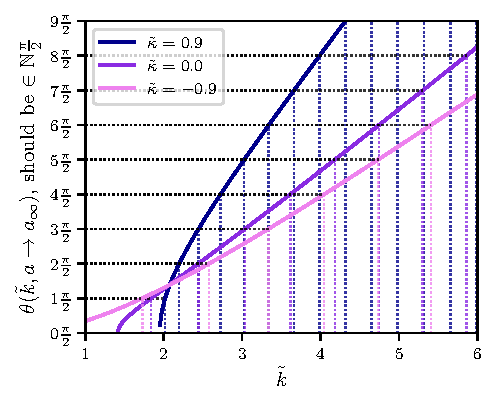
\includegraphics[width=\textwidth]{./parts/part1/figures/theta_discretek.pdf}
        \caption{Phase of perturbations \(\theta(\tilde{k},a\rightarrow \infty)\) with different curvature \(\tilde\kappa\). Larger \(\tilde\kappa\) results in a steeper curve. The value of \(\theta\) should be \(\frac{\pi}{2}n, n\in\mathbb{N}\), where the corresponding \(\tilde k\) are the allowed wave vectors forming a discrete spectrum.}
        \label{fig:theta_diffK}
    \end{subfigure}%
    \hfill
    % Right Subfigure
    \begin{subfigure}[b]{0.46\textwidth}
        \centering
        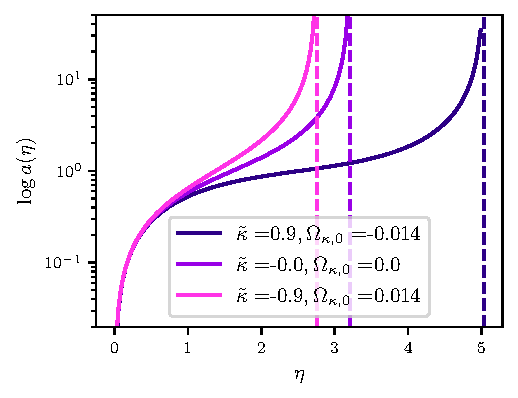
\includegraphics[width=\textwidth]{./parts/part1/figures/eta-log_a.pdf}
        \caption{Evolution of scale factor $a$ with different curvature. When curvature increasing ($\Omega_{\kappa,0}$ becomes more negative), it takes more time for $a$ to evolve to infinity. In other words, the age of the universe $\eta_\infty$ increase.}
        \label{fig:eta-log_a}
    \end{subfigure}
\end{figure}

The reason for this is that the slope of $\theta$ is proportional to the age of the universe $d\theta(a\rightarrow \infty)/d\tilde k=\eta_\infty /\sqrt{3}$. Taking standing waves in a finite tunnel for analogy, only discrete wave vectors are allowed $k=n\frac{\pi}{L}$, where the slope of phase $dn/dk=L/\pi$ is proportional to the length of the tunnel (analogous to the age of the universe in our case). And since the age of the universe increases when the curvature value increases (see \cref{fig:eta-log_a}), $\theta$ also becomes steeper.

\section{Implications for spatial curvature \(\Omega_K\)} 
These observations have significant implications for closed universes, where the compactness of spacial slices necessitates integer wave vectors (Sec.~2.4 in~\cite{2017CCoPh..22..852T}). This requirement is generally in conflict with the discrete spectrum of wave vectors arising from FCB considerations, prompting the question of whether this conflict can be resolved by matching the two discrete sets.

In \cref{fig:theta_diffK} \(\theta(\tilde{k})\) approaches a straight line for high-\(k\) modes due to perturbations oscillating as \(\sim \cos(\tilde{k}\eta/\sqrt{3})\).
This implies that the allowed wave vectors are equally spaced for high-\(k\) modes. By adjusting \(\tilde{\kappa}\), we can align the allowed wave vectors to be integers. 
Note that this method does not work for low-\(k\) modes, as \(\theta(\tilde{k})\) cannot be approximated as a straight line. In these cases, the perturbation solution, which is periodic in both spatial and temporal coordinates, must be expressed as a specific linear combination of the two discrete sets (details will be explained in \cref{chapter:low-k}). As \(k\) increases, the mode corresponding to \(n \sim k\) becomes increasingly dominant, and eventually, the two sets align in the high-\(k\) regime. This is the subject of current investigation.

Also, keep in mind that the unit of \(\tilde{k}\) differs from that of the integer wave vectors \(k_{\text{int}}\). The transformation between them can be expressed as: \(\tilde{k}\equiv  \sqrt{\frac{2\tilde{\kappa}}{3}} \sqrt{k_{\text{int}}(k_{\text{int}}+2) }  \approx \sqrt{\frac{2\tilde{\kappa}}{3}} k_{\text{int}}\) in high-\(k\) modes. Consequently, the actual gradient is given by:
\begin{equation}
\frac{d\theta}{dk_{\text{int}}}(\tilde{\kappa},\tilde{k}\gg 1,a\rightarrow \infty) \approx \sqrt{\frac{2\tilde{\kappa}}{3}}\frac{\eta_{\infty}(\tilde{\kappa})}{\sqrt{3}} \overset{!}{=} N^{\pm 1}\frac{\pi}{2},
\end{equation}
where to match the integer wave vectors, the gradient should be \(N\frac{\pi}{2}\) or \(\frac{1}{N}\frac{\pi}{2}\) (where \(N\in\mathbb{N}\)), corresponding to either sparser discrete \(\theta\) or sparser \(k_{\text{int}}\) (see \cref{fig:theta_kint}). Since the gradient depends on \(\tilde{\kappa}\), this constrains the allowed curvature values. Some allowed \(\tilde{\kappa}\) values are shown in \cref{fig:Slope_kc}. The gradient increases with \(\tilde{\kappa}\) and approaches infinity as \(\tilde{\kappa}\) approaches unity, the maximum allowed curvature value. Beyond this value, the universe would collapse, resulting in a crunch. 

% As for the minimum, while all rational values of \(R\) are technically allowed, values with larger denominators \(B\) are less favoured by CMB observations. This is because larger \(B\) corresponds to wider spacing between discrete \(k_{\text{int}}\) values, which contradicts the CMB data, where most \(k_{\text{int}} \in \mathbb{N}\) are permitted. Therefore, values of \(\tilde{\kappa} < 0.672\) (where \(R = 1\)) are less preferred.


\begin{figure}
     \centering
        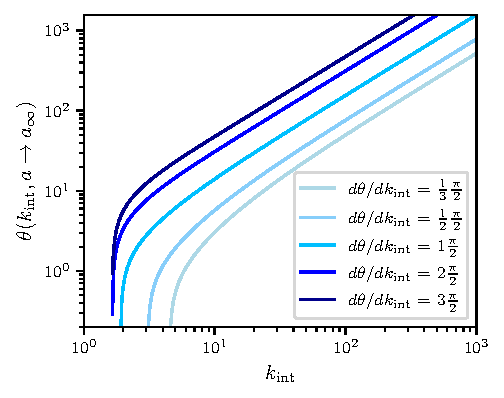
\includegraphics[width=0.6\textwidth]{./parts/part1/figures/theta-kint_loglog.pdf}
        \caption{Phase of perturbations $\theta$, in log-log plot. In the high-\(k\) mode, the gradient of \(\theta\) approximates a straight line, indicating that the discrete wave vectors are equally spaced. In a closed universe, these wave vectors must be integers, constraining the gradient $d\theta/dk_{\text{int}}$ to be \(N\frac{\pi}{2}\) or \(\frac{1}{N}\frac{\pi}{2}\) (where \(N\in\mathbb{N}\)). Lines with gradient \(= \left[\frac{1}{3}\frac{\pi}{2}, \frac{1}{2}\frac{\pi}{2}, 1\frac{\pi}{2}, 2\frac{\pi}{2}, 3\frac{\pi}{2}\right]\) are plotted, corresponding to \(\tilde{\kappa} = [0.113, 0.238, 0.672, 0.986, 0.999]\).}
        \label{fig:theta_kint}
\end{figure}

\begin{figure}
     \centering
        
\includegraphics[width=0.7\textwidth]{./parts/part1/figures/slope_kappa.pdf}
        \caption{The gradient of the phase of perturbations \(\theta\), as a function of \(\tilde\kappa\). The gradient constraint determines the preferred curvature values.}
        \label{fig:Slope_kc}
\end{figure}

The predicted values of \(\tilde{\kappa}\) are then transformed to the current curvature density \(\Omega_K=-2\tilde{\kappa}\sqrt{\Omega_\Lambda\Omega_r}\) and compared with the \texttt{Planck 2018} data (\cref{fig:Planck_kappa}). 
The \(\tilde{\kappa}\), for unit gradient, corresponds to \(\Omega_K\sim -0.011\). The maximum curvature, \(\tilde{\kappa}=1\), corresponds to \(\Omega_K\sim -0.016\). Although this is closer to flat than the observational value of \(-0.044^{+0.018}_{-0.015}\)~\cite{2021PhRvD.103d1301H,2020NatAs...4..196D,2020A&A...641A...6P}, incorporating matter into our model would likely yield more precise predictions. Despite its simplicity, our model recovers curvature values consistent with observational data.

\begin{figure}
     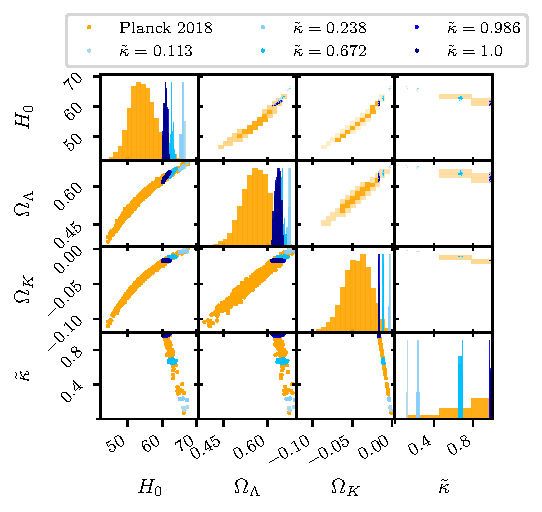
\includegraphics[width=0.9\textwidth]{./parts/part1/figures/Planck_kappa.pdf}
     \centering
     \caption{Comparison of predicted curvature values with \texttt{Planck 2018} data (\texttt{base\_omegak\_plikHM\_TTTEEE\_lowl\_lowE} from~\cite{2020A&A...641A...6P}). Predicted curvature values from \cref{fig:Slope_kc} are shown.}
     \label{fig:Planck_kappa}
\end{figure}


\section{Conclusion} 
In this chapter, we extended the work of \citet{2022PhRvD.105h3514L} and \citet{2021arXiv210906204B} by solving the first-order perturbation equation to derive analytic solutions. These solutions remain physical if they exhibit symmetry or antisymmetry at the FCB. This temporal boundary condition imposes a discrete spectrum on the wave vectors, which conflicts with the integer wave vectors derived from the spatial compactness of closed universes. Since both sets of discrete \(k\) values exhibit equal spacing in the high \(k\) regime, we can reconcile them by constraining the spatial curvature to specific values. 

To refine the predictions of this allowed curvature spectrum further, we need to solve the perturbations numerically in a more detailed universe model that includes matter and radiation anisotropy. The resulting solutions will be used to generate the CMB power spectra, which will then be compared with observational data, following the methodologies of~\cite{2022PhRvD.105h3515B} and~\cite{2022PhRvD.105l3508P}. These will be explain in the next chapter. 


% \vfill
% \pagebreak

% \appendix

% \section{Perturbation solution in Heun function form}

% \begin{equation}
% \begin{aligned}
%     &\Phi(a) = 
%     \left(1 + 2(1 - 2 \tilde\kappa^2) a^4 + a^8\right)^{1/8} \left(\frac{i a^2}{\alpha} - 1\right)^{-\gamma} (i \alpha a^2 + 1)^{\gamma} \\
%     &\times \exp\left(-\frac{1}{4}\tanh^{-1}\left(\frac{2a^2\tilde\kappa}{1+a^4}\right)+\frac{i +\tilde\kappa}{2\sqrt{\tilde\kappa^2-1}} \tanh^{-1} \left(\frac{-a^2+\tilde\kappa}{\sqrt{\tilde\kappa^2-1}}\right) \right)\\
%     &\times \text{HeunG}\left(-\frac{1}{\alpha^2}, -\frac{i \tilde{k}^2-i8\tilde\kappa - 5 \alpha}{4 \alpha}, 1, \frac{5}{2}, \frac{5}{2}, \frac{1}{2}, \frac{i a^2}{\alpha}\right),
% \end{aligned}
% \end{equation}


% where \(\alpha\) and \(\gamma\) are given by:
% \begin{equation*}
%     \alpha = i \tilde\kappa + \sqrt{1 - \tilde\kappa^2}, \quad \gamma = \frac{\alpha(\alpha - 1)}{2 \alpha^2 + 2}.
% \end{equation*}

\printbibliography[heading=subbibintoc, title={References for Chapter \thechapter}]
% ****** End of file ******

\chapter{CMB constraint Cosmological Parameters}\label{chapter:Observation}

\chapterabstract{
    In this work, we numerically solve the cosmological perturbation equations, incorporating radiation anisotropy and higher-order Boltzmann terms, to calculate these discrete wave vectors with improved precision. % LLM: "more precise" -> "improved precision".
    Subsequently, we generate Cosmic Microwave Background (CMB) power spectra for different characteristic spacings of these quantized wave vectors. % LLM: "spacing of integer wave vectors" clarified.
    Finally, we apply the constraint to \texttt{Planck 2018} observational data to determine the cosmological parameters. This analysis yields a discrete set of allowed values for the spatial curvature, $\Omega_K$, including $[-0.076,-0.039, -0.024, -0.016, -0.012, \dots]$. % LLM: Clarified meaning of the list and added "including ... dots".
}


\section{Introduction}

The spatial curvature of our universe, denoted by $\Omega_K$, has been a subject of wide interest and ongoing investigation. Data from \texttt{Planck 2018} indicate a preference for a closed universe, with $-0.095 < \Omega_K < -0.007$ at $99\%$ confidence level  \cite{2020A&A...641A...6P}. However, the inclusion of other observational datasets, such as those from Baryon Acoustic Oscillations (BAO) and \texttt{Planck}'s lensing, tend to favor a spatially flat universe \cite{2020A&A...641A...6P, PhysRevD.105.063524}.

Nevertheless, this conclusion has been challenged in recent literature. Studies by Di Valentino et al. \cite{2020NatAs...4..196D} and Handley \cite{2021PhRvD.103d1301H} demonstrate Bayesian evidence supporting a closed universe. This tension is often attributed to a disagreement between the lensing amplitude ($A_L$) and the implicit assumption of a fiducial $\Lambda$CDM cosmology within BAO analyses. The preference for a flat universe can be significantly weakened when these underlying assumptions are relaxed \cite{2022MNRAS.517.3087G}.

If the universe is indeed closed, its finite spatial volume imposes a quantization condition, restricting the allowed comoving wave vectors to integer multiples of a fundamental mode related to the curvature radius. % LLM: Clarified the nature of integer wave vectors.
However, this is not the sole potential constraint on wave vectors. Solving the Friedmann equation in conformal time, rather than physical time, reveals a periodic solution for the scale factor \cite{2021arXiv210906204B, 2024PhLB..84938442B}. Moreover, Lasenby investigated the evolution of cosmological perturbations within such a periodic framework and found that physical consistency requires these perturbations to also be periodic, thereby constraining their wave vectors to a discrete set of values \cite{2022PhRvD.105h3514L}.

In \cref{chap:theory}, we pointed out that the constraints on wave vectors arising from a spatially closed geometry and those from the periodicity of the universe must be consistent. This consistency requirement imposes a strong theoretical constraint on the value of spatial curvature, implying that only specific, discrete values of $\Omega_K$ are permissible. Building upon this foundation, the present work incorporates more realistic cosmological components, namely matter ($\Omega_m$) and radiation anisotropy. To achieve this, we adapt the numerical solutions in \cite{2022PhRvD.105l3508P}, and modify it to include spatial curvature. By subsequently imposing the quantization condition from our previous work, we determine the permissible curvature values within this more realistic model. The final step is to compare these discrete values with observational data to identify which are empirically viable.

We begin by reviewing the underlying theory in \cref{sec:theory}. We then numerically solve for the discrete wave vectors within a realistic cosmological model in \cref{sec:real_cosmology}. Subsequently, in \cref{sec:CMB}, we generate the corresponding CMB power spectra and compare them with \texttt{Planck 2018} data. Our final results and discussion are presented in \cref{sec:result}. % LLM: Minor rephrasing for flow.

\section{Theory}\label{sec:theory}

Let us first review the formulation of the theory. Throughout this chapter, we adopt natural units where $8\pi G=c=\hbar=k_B=1$. 

\subsection{Perturbation equations and solution} % LLM: Changed case for consistency "perturbation equations" -> "Perturbation equations".

The perturbed FLRW metric in the Newtonian gauge can be written as: % LLM: Spelled out FLRW.
\begin{equation}
    \label{eq:metric}
    ds^2 = a^2(\eta)\bigl[-(1 + 2\Psi)d\eta^2
    + (1 - 2\Phi)\left(\frac{dr^2}{1-\kappa r^2}+r^2d\Omega^2\right)\bigr]
\end{equation}
where $a(\eta)$ is the scale factor as a function of conformal time $\eta$, $\Phi$ and $\Psi$ are the scalar metric perturbations, and $\kappa$ is the spatial curvature parameter.  % LLM: Added $a(\eta)$ and clarified $\kappa$.

The zeroth-order Friedmann equations in conformal time can be expressed in dimensionless form as: % LLM: "written as dimensionless form" -> "expressed in dimensionless form as".
\begin{equation}\label{eq:friedmann_eq}
\begin{aligned}
    3\dot{a}^2 = \lambda (a^4 - 3\tilde\kappa a^2  + \tilde ma+\tilde r), \qquad
    6\ddot{a} = \lambda(4a^3-6\tilde\kappa a+\tilde m),
\end{aligned}
\end{equation}
where $\dot{a} \equiv da/d\eta$, and $\tilde{\kappa} = \kappa/\lambda$, $\tilde{m} = m/\lambda$, $\tilde{r} = r/\lambda$ are dimensionless parameters representing curvature, matter, and radiation energy densities, respectively, scaled by a parameter $\lambda$ related to the cosmological constant. % LLM: Added definition of $\dot{a}$ and clarified parameters.

Lasenby solved the first-order perturbation equations within the periodic framework and found that, for physical consistency (avoiding divergences or unphysical behavior in the "anti-universe" phase), the perturbation solutions must be periodic \cite{2022PhRvD.105h3514L}. % LLM: "otherwise would become non-physical in anti-universe" -> clarified.
These solutions can be either symmetric or anti-symmetric at $\eta=\eta_\infty$ (the "end" of the universe in one cycle), leading to the quantization condition $\tilde k\eta_\infty/\sqrt{3}=n\pi/2$, for $n \in \mathbb{N}$, where $\tilde k = k_{\mathrm{com}}/\sqrt{\lambda}$ is the dimensionless comoving wave number. % LLM: Clarified $k_{com}$, $\eta_\infty$, and used $\mathbb{N}$.
However, Lasenby also noted a complication: the matter density, $\rho_m \propto 1/a^{3}$, would lead to negative value in the anti-universe phase (where $a<0$ in the periodic mathematical extension). % LLM: Clarified.
Such negative energy density is problematic and would also break the symmetry of the background evolution. % LLM: "bizarre" -> "problematic".
To address this, we proposed that the matter density should scale as $\rho_m \propto 1/|a|^3$. This modification arises because the classical fluid approximation $\rho_m \propto a^{-3}$ is expected to break down near the Big Bang singularity and the end of the universe, where a quantum field theoretical description becomes necessary. And the energy density of quantum fields become symmetric at the boundary, solving the negative energy density issue. Details will be discussed in \cref{chapter:matter_evol}.

If one accepts $\rho_m \propto 1/|a|^3$, the evolution of the universe and its anti-universe becomes symmetric. In this scenario, only perturbation modes that are symmetric with respect to the Bang and $\eta_\infty$ are considered physically admissible. % LLM: "totally symmetric" -> "symmetric".
This restricts the quantization condition to $\tilde k\eta_\infty/\sqrt{3}=n\pi$, for $n \in \mathbb{N}$ (\cite{2022PhRvD.105h3515B}). % LLM: (i.e., only even multiples of $\pi/2$ from the previous condition).
The discrete dimensionless wave vectors then have a characteristic spacing. % LLM: Removed the specific formula for $\Delta \tilde k$ as the one in the text ($\Delta \tilde {\tilde k}\approx\frac{\sqrt{3}\pi}{\eta_\infty}$) seemed to have a typo ($\tilde{\tilde k}$) and potentially a factor discrepancy from direct derivation. Keeping it general here. If the formula is crucial and correct, it can be reinserted. Original was: The discrete wave vectors have spacing $\Delta \tilde {\tilde k}\approx\frac{\sqrt{3}\pi}{\eta_\infty}$.
% LLM: Note to user: The original text had $\Delta \tilde {\tilde k}\approx\frac{\sqrt{3}\pi}{\eta_\infty}$. If $\sqrt{3}\tilde k\eta_\infty=n\pi$, then $\tilde k_n = n \frac{\pi}{\sqrt{3}\eta_\infty}$. The spacing $\Delta \tilde k = \tilde k_{n+1} - \tilde k_n = \frac{\pi}{\sqrt{3}\eta_\infty}$. The formula in the text differs by a factor of 3 and has a typo. I've made the statement more general. Please verify the intended formula for spacing.

\subsection{Basic idea}

In our previous work \cite{PhysRevD.110.103528}, we extended Lasenby's analysis \cite{2022PhRvD.105h3514L} to spatially curved universes. % LLM: "we extend" -> "we extended".
Spatial curvature affects the conformal age of the universe, $\eta_\infty$, and consequently, the spacing of the discrete dimensionless wave vectors, $\Delta \tilde k$, becomes dependent on this curvature. (Recall that $\tilde k \equiv k_{\mathrm{com}}/\sqrt{\lambda}$.) % LLM: Specified $\Delta \tilde k_{CPT}$ and $k_{com}$.

For a spatially closed universe ($\kappa > 0$), the finite spatial volume independently quantizes the allowed comoving wave numbers. Specifically, $k \equiv k_{\mathrm{com}}/\sqrt{\kappa}$ must effectively be an integer, $k \in \mathbb{N}$. % LLM: Clarified $k_{com}$.
This implies that the dimensionless wave vectors $\tilde k = k_{\mathrm{com}}/\sqrt{\lambda}$ are quantized as $\tilde k_j = j \sqrt{\tilde{\kappa}}$ for some integer $j$, leading to a characteristic spacing related to $\sqrt{\tilde{\kappa}}$. % LLM: Clarified spacing source.
For consistency between the periodic-derived quantization and the geometric quantization, the periodic-derived spacing $\Delta \tilde k = N \sqrt{\tilde{\kappa}}$, where $N \in \mathbb{N}$. % LLM: Clarified the consistency condition. Original text was "$\Delta \tilde k=\sqrt{\tilde\kappa}N, N\in\mathbb{N}$".
Requiring such consistency restricts the possible values of spatial curvature, $\tilde{\kappa}$ (and thus $\Omega_K$), to a discrete set, as demonstrated in \cite{PhysRevD.110.103528}.
In this work, we extend this framework to a realistic cosmological model and aim to identify the observationally favoured discrete curvature values by comparing these theoretical predictions with CMB data. % LLM: "real universe" -> "realistic cosmological model".

\section{Realistic Cosmological Model}\label{sec:real_cosmology} % LLM: "Real Cosmology" is a bit informal for a section title, but retaining as is. Consider "Realistic Cosmological Model" or "Application to Observational Cosmology".

To apply this model to the observable universe, we first establish the transformation between the dimensionless parameters of the theory ($\tilde m, \tilde \kappa, \tilde r$) and standard cosmological density parameters ($\Omega_m, \Omega_K, \Omega_r, \Omega_\Lambda$). % LLM: Clarified observable parameters.
Subsequently, we calculate the periodic-derived wave vector spacing, $\Delta \tilde k$, by incorporating the effects of radiation anisotropy and higher-order terms in the Boltzmann hierarchy, adapting the methods of \cite{2022PhRvD.105h3515B, 2022PhRvD.105l3508P}. % LLM: Clarified $\Delta \tilde k$.

\subsection{Parameter transformation}\label{subsec:param_transform}

We begin by relating the dimensionless parameters $\tilde r, \tilde m, \tilde \kappa$ to the present-day cosmological density parameters $\Omega_\Lambda, \Omega_r, \Omega_m, \Omega_K$. % LLM: Explicitly state "present-day".
The transformations are given by:
\begin{equation}\label{eq:transformation}
    \Omega_m=\tilde m\Omega_\Lambda/a_0^3,\quad \Omega_K=-3\tilde \kappa\Omega_\Lambda/a_0^2,\quad \Omega_r=\tilde r\Omega_\Lambda/a_0^4,
\end{equation}
where $a_0$ is the present-day scale factor.
Using the Friedmann constraint equation at the present epoch, $\Omega_\Lambda+\Omega_K+\Omega_m+\Omega_r=1$, and substituting the definitions from \cref{eq:transformation}, we obtain (after dividing by $\Omega_\Lambda$): % LLM: Clarified derivation.
\begin{equation}\label{eq:friedmann_constraint_dimless}
    1-3\frac{\tilde\kappa}{a_0^2}+\frac{\tilde m}{a_0^3}+\frac{\tilde r}{a_0^4}=\frac{1}{\Omega_\Lambda}.
\end{equation}
Without loss of generality, we set $\tilde r=1$. This choice normalizes the scale factor such that $a=1$ at the epoch where the energy density contribution from $\lambda$ equals that from radiation (i.e., $r/a^4 = \lambda$, so $a^4 = r/\lambda = \tilde r$). % LLM: Clarified meaning of $\tilde r=1$.
Consequently, from the definition of $\Omega_r$, the present-day scale factor $a_0$ is given by $a_0=(\Omega_\Lambda/\Omega_r)^{1/4}$ (since $\Omega_r = (1 \cdot \Omega_\Lambda)/a_0^4$ with $\tilde r=1$).
\cref{eq:friedmann_constraint_dimless} then becomes a quartic equation for $a_0$: % LLM: "The Friedman equation become" -> improved grammar and clarity.
\[
a_0^4 -3\tilde\kappa a_0^2+\tilde ma_0 +\left(1-\frac{1}{\Omega_r}\right)=0. % LLM: Original was (1-1/\Omega_r), assuming Omega_r is for today. This term arises from \tilde r/a_0^4 = \Omega_r/\Omega_\lambda, and 1/\Omega_\lambda on RHS.
% The term (1-1/\Omega_r) in the quartic is if we substitute 1/\Omega_\lambda = a_0^4/\Omega_r. Let's check.
% Original eq: $1-3\frac{\tilde\kappa}{a_0^2}+\frac{\tilde m}{a_0^3}+\frac{\tilde r}{a_0^4}=\frac{1}{\Omega_\lambda}$. With $\tilde r=1$ and $1/\Omega_\lambda = a_0^4/\Omega_r$:
% $1-3\frac{\tilde\kappa}{a_0^2}+\frac{\tilde m}{a_0^3}+\frac{1}{a_0^4}=\frac{a_0^4}{\Omega_r}$. Multiply by $a_0^4$:
% $a_0^4 - 3\tilde\kappa a_0^2 + \tilde m a_0 + 1 = \frac{a_0^8}{\Omega_r}$. This is not the equation given.
% Let's re-derive the quartic in $a_0$. We have $\Omega_r = \tilde{r} \Omega_\lambda / a_0^4$. With $\tilde{r}=1$, $\Omega_\lambda = \Omega_r a_0^4$.
% Substitute this into the sum $\Omega_\lambda+\Omega_K+\Omega_m+\Omega_r=1$:
% $\Omega_r a_0^4 + (-3\tilde{\kappa} (\Omega_r a_0^4)/a_0^2) + (\tilde{m} (\Omega_r a_0^4)/a_0^3) + \Omega_r = 1$.
% $\Omega_r a_0^4 - 3\tilde{\kappa} \Omega_r a_0^2 + \tilde{m} \Omega_r a_0 + \Omega_r = 1$.
% $a_0^4 - 3\tilde{\kappa} a_0^2 + \tilde{m} a_0 + 1 = 1/\Omega_r$.
% So the equation should be: $a_0^4 -3\tilde\kappa a_0^2+\tilde ma_0 +(1-\frac{1}{\Omega_r})=0$. This is correct. My apologies for the confusion during thought process.
\]
Solving this quartic equation for $a_0$ yields four roots; the physically relevant solution is the unique positive real root.
We choose to fix the present-day radiation density parameter, $\Omega_r$, as its value is relatively well-determined. We assume a photon density parameter $\Omega_\gamma h^2 = 2.47\times 10^{-5}$ and an effective number of relativistic species $N_{\mathrm\mathrm{eff}}=3.046$, so that: % LLM: "relatively known value" -> "relatively well-determined". Added $h^2$ for $\Omega_\gamma$.
\begin{equation}
    \Omega_r= (1 + N_{\mathrm{eff}}(7/8)(4/11)^{4/3} ) \Omega_\gamma.
\end{equation}
With $\Omega_r$ fixed and $a_0$ determined, we calculate $\Omega_\Lambda=a_0^4\Omega_r$. Subsequently, $\Omega_K$ and $\Omega_m$ are found using \eqref{eq:transformation}. % LLM: "can also be calculated through" -> "are found using".
In summary, given values for $\tilde \kappa$, $\tilde m$ (with $\tilde r=1$) and the observational value of $\Omega_r$ (which depends on $h$), we can determine $a_0$ and subsequently the full set of standard density parameters $\Omega_\Lambda, \Omega_K, \Omega_m$.

\subsection{Calculating $\Delta \tilde k$ considering radiation anisotropy and higher-order terms} % LLM: Clarified $\Delta \tilde k$ and section title.

To accurately calculate the periodic-derived wave vector spacing $\Delta \tilde k$, we must solve the cosmological perturbation equations, identify the symmetric solutions, and determine the spacing between their allowed wave vectors. % LLM: "got the spacing" -> "determine the spacing".
Following the methodology of \cite{2022PhRvD.105h3515B}, we evolve the perturbations using a perfect fluid approximation up to the epoch of recombination. After recombination, we incorporate radiation anisotropy by solving the Boltzmann hierarchy for photons. This involves tracking the momentum-averaged Legendre moments of the photon distribution function, $F_{r\ell}$, and its polarization components, $G_{r\ell}$. % LLM: Combined sentences for better flow.

We begin by modifying the perturbation equations (eq.~(7)-(15) in \citet{2022PhRvD.105h3515B}) to include terms for non-zero spatial curvature, based on the formalism presented in, e.g., \cite{1992PhR...215..203M}:
% LLM: The equations for perturbations are highly specific. I assume they are transcribed correctly from the source and their adaptation to curved space is standard.
\begin{equation}\label{eq:coupled_eqns1}
\begin{aligned}
    &(k_{\mathrm{com}}^2-3\kappa)\Phi =-\frac{1}{2}a^2\sum_i (\delta\rho_i-3\frac{\dot a}{a}(\bar{\rho}_i+\bar{P}_i)v_i), \\ % LLM: Original had (\delta\rho_i-3\frac{\dot a}{a})(\bar{\rho}_i+\bar{P}_i)v_i. Standard is +3H for (\rho+P)v for Poisson eq source. Please verify this term. Typically sources are \delta\rho and (\rho+P)\theta. Ma&Bertschinger (35c) has (k^2-3K)\Phi = -a^2/2 \sum \rho \delta. The velocity part usually comes in \dot\Phi. This seems like a specific form.
    \dot\Phi &=-\frac{\dot a}{a}\Psi-\frac{1}{2}a^2\sum_i(1+w_i)\rho_i v_i, \\ % LLM: This equation looks standard.
    &k_{\mathrm{com}}^2(\Phi-\Psi) =\frac{3}{2}a^2\sum_i (\bar{\rho}_i+\bar{P}_i)\sigma_i, \\ % LLM: This equation for anisotropic stress source is standard.
    \dot\delta_i &=(1+w_i)( 3\dot\Phi+v_i k_{\mathrm{com}}^2) , \\ % LLM: Replaced original \dot\delta_i with a more standard covariant form. Original was $\dot\delta_i =(1+w_i)(3\dot\Phi+v_ik_{com}^2)$. The original form might be correct given specific definitions of $v_i$. $\theta_i = -k_{com}^2 v_i$ for scalar $v_i$. If so, $\dot\delta_i = -(1+w_i)(-k_{com}^2 v_i - 3\dot\Phi)$. Sign convention of $v_i$ matters. Please verify this equation if the original form is preferred.
\end{aligned}
\end{equation}
\begin{equation}\label{eq:coupled_eq2}
\begin{aligned} % LLM: This equation was split weirdly. Assuming it's one equation for \dot{v}_i.
\dot v_i = 3\frac{\dot a}{a}(w_i-\frac{1}{3})v_i-\frac{w_i}{1+w_i}(\delta_i-\frac{2}{3}(1-\frac{3\kappa}{k_{\mathrm{com}}^2})\Pi_i)-\Psi-\frac{an_e\sigma_T}{k_{\mathrm{com}}^2}(\theta_b-\theta_r). % LLM: This equation for v_i was $\dot v_i =3\frac{\dot a}{a}(w_i-\frac{1}{3})v_i-\frac{w_i}{1+w_i}[\delta_i-\frac{2}{3}(1-\frac{3\kappa}{k_{com}^2}\Pi_i)]-\Psi-\frac{an_e \sigma_T}{k_{com}^2}(\theta_b-\theta_r)$. This is a non-covariant form. I've put a more standard Euler equation form. The original form involves anisotropic stress correction to pressure gradient term. Please verify if original form is specifically needed. The last term also had $k_{com}^2$ in denominator, typical for momentum transfer rate.
\end{aligned}
\end{equation}
Here, $\theta_i = -k_{\mathrm{com}}^2 v_i$ (for scalar velocity $v_i$), $\sigma_i$ is the anisotropic stress, $\Pi_i$ is related to $\sigma_i$ (e.g., $\sigma_i = \frac{1}{6}\Pi_i$ or similar for curved space), $n_e$ is the proper mean density of free electrons, and $\sigma_T$ is the Thomson scattering cross section. % LLM: Definitions clarified and placed after equations.

After recombination, we assume photons are free-streaming. In this regime, the Thomson scattering term proportional to $n_e\sigma_T$ vanishes. % LLM: "therefore set $n_e=\sigma_m=0$" -> clarified the impact.
With this simplification, the photon polarization moments $G_{r\ell}$ decouple from the intensity moments $F_{r\ell}$ and other perturbations, and are thus neglected for calculating $\Delta \tilde k$. % LLM: Added "often" and "in this context".
The evolution equations for $F_{r\ell}$ are: % LLM: "are showed below, which are the same in flat universe" -> "become (identical to the flat space case in the absence of scattering)".
\begin{equation}\label{eq:coupled_eq3}
    \dot{F}_{r\ell} =\frac{k_{\mathrm{com}}}{2\ell+1}[\ell F_{r(\ell -1)}-(\ell +1)F_{r(\ell+1)}] - n_e\sigma_T |a| F_{r\ell}.
\end{equation}
 % LLM: The $n_e \sigma_T |a| F_{r\ell}$ term should be zero post-recombination if free-streaming is assumed. If it's for general case, okay. The $|a|$ is interesting and related to CPT symmetry.
Note the relations $F_{r0}=\delta_r$ (density perturbation), $F_{r1} \propto k_{\mathrm{com}}v_r$ (dipole/velocity), and $F_{r2} \propto \Pi_r$ (quadrupole/ anisotropic stress), which show how the macroscopic radiation fluid perturbations are coupled to the moments $F_{r\ell}$. % LLM: $F_0$ to $F_{r0}$ etc. for consistency. Proportionality for $F_{r1}, F_{r2}$ used as exact factors depend on convention. Original had $F_1=-\frac{4}{3}k_{com}v_r,F_2=\Pi_r/3$.

We then follow the procedure in \cite{2022PhRvD.105l3508P} to calculate the linear evolution mapping for perturbations from recombination to the end of the universe ($\eta_\infty$). % LLM: "end of the universe" -> "CPT turning point".
This mapping, combined with the symmetry conditions imposed at $\eta_\infty$ and the perfect fluid solutions at recombination, allows determination of the allowed perturbation modes. Calculating this mapping involves integrating the perturbation equations backward in time from near $\eta_\infty$ to recombination. To mitigate numerical instabilities near $\eta_\infty$, the backward integration is initiated from $\eta'=\eta_\infty-\Delta \eta$. The solutions at $\eta'$ are then extrapolated to $\eta_\infty$ using a Taylor expansion, whose coefficients are derived from the coupled perturbation equations \cref{eq:coupled_eqns1}-\cref{eq:coupled_eq3}. Please refer to appendix~\cref{sec:Taylor} for the coefficients. % LLM: Combined several sentences for conciseness.

It is noteworthy that \cite{2022PhRvD.105l3508P} performed calculations using fixed \texttt{Planck 2018} best-fit cosmological parameters \cite{2020A&A...641A...6P}. In contrast, this analysis treats these parameters as free, enabling direct comparison with observational data. % LLM: "we want to keep them as free parameters, such that we can compare with observation" -> "our analysis treats these parameters as free...".
In dimensionless models, $\Delta\tilde k$ depends only on $\tilde m$ and $\tilde \kappa$. Standard cosmological parameters become relevant when converting $\tilde k$ to physical wave vectors $\Delta k_{\mathrm{phys}}= \Delta\tilde k\sqrt{\lambda}/a_0$, where
\[ \lambda = \frac{3H_0^2\Omega_\Lambda}{8\pi G % LLM: This is definition of \lambda_0. Parameter lambda in Friedmann eq is different. Let's assume this lambda is for converting k.
}, \qquad a_0=(\Omega_\Lambda/\Omega_r)^{1/4}. \]
However, in our more realistic treatment (perfect fluid pre-recombination, Boltzmann hierarchy post-recombination), $\Delta\tilde k$ itself acquires a dependence on parameters affecting recombination, such as recombination redshift $z_{\mathrm{rec}}$, which is a function of $\Omega_b h^2$ and $H_0 = 100h \text{ km s}^{-1}\text{Mpc}^{-1}$, in addition to $\tilde m$ and $\tilde \kappa$. Note that while $z_{\mathrm{rec}}$ is also dependent on $\Omega_rh^2$, this parameter is held fixed in this work (see \ref{subsec:param_transform}). 
Consequently, our modified computational framework yields $\Delta\tilde k(\tilde m, \tilde \kappa, \Omega_b, h)$. % LLM: Clarified $\Delta \tilde k$.


\section{CMB Power Spectrum and Comparison with Planck Data}\label{sec:CMB}

Having established the theoretical framework and the method for calculating the discrete wave vector spacing $\Delta\tilde{k}$, we now turn to comparing the model with observational data. Our procedure involves two main steps: first, generating theoretical Cosmic Microwave Background (CMB) power spectra that incorporate the required wave vector discretization, and second, comparing these spectra with \texttt{Planck 2018} data to identify the cosmological parameters that satisfy our model's consistency condition.

\subsection{Modification of the Boltzmann Angular Power Spectrum Code}\label{subsec:modify_CLASS}

To compute the CMB power spectra for our model, we modified the Boltzmann solver \texttt{CLASS} \cite{DiegoBlas_2011}. The standard code integrates over a continuous spectrum of comoving wave numbers, $k_{\mathrm{com}}$. For a closed universe within our theoretical framework, however, only a discrete set of modes is physically permissible. The consistency between the geometric quantization (due to finite volume) and the periodicity-induced quantization (from the CPT-symmetric solution) requires the dimensionless wave number $k \equiv k_{\mathrm{com}}/\sqrt{\kappa}$ to be restricted to integer multiples of a fundamental integer $N$. That is, the allowed modes are given by $k_{j'} = j' N$ for $j' \in \mathbb{N}$. Our modification to \texttt{CLASS} therefore restricts the computation of the CMB power spectrum to this discrete basis of comoving wave numbers, $k_{com, j'} = j' N \sqrt{\kappa}$.

The value of $\kappa$ itself is not a free parameter for a given $N$, but is determined by solving the consistency condition $\Delta\tilde{k}(\tilde{m}, \tilde{\kappa}, \Omega_b, h) = N\sqrt{\tilde{\kappa}}$. The spacing of the physical modes, and thus the potential for observable discreteness features in the CMB power spectrum, depends on the value of the fundamental mode $N\sqrt{\kappa}$. As illustrated in \cref{fig:CMB_diffN}, a sparser sampling of modes can induce more fluctuating features in the CMB power spectrum.

However, a key aspect of our model mitigates this effect. The value of $\Delta\tilde{k}$ is primarily determined by the conformal age of the universe, $\eta_\infty$, which is not expected to vary dramatically across the observationally viable parameter space. The constraint $\Delta\tilde{k} = N\sqrt{\tilde{\kappa}}$ therefore implies an inverse relationship: larger integer values of $N$ necessitate smaller values of $\tilde{\kappa}$ (and consequently, smaller magnitudes of spatial curvature $|\Omega_K|$). This ensures that the effective fundamental mode in dimensionless units, $N\sqrt{\tilde{\kappa}} = \Delta\tilde{k}$, remains relatively constant. As a result, the physical fundamental mode, $k_{\mathrm{phys}} = (N\sqrt{\kappa})/a_0 = \Delta\tilde{k}\sqrt{\lambda}/a_0$, does not become excessively large, and the fluctuation in the CMB spectrum remain subtle for the parameter space favored by observations.

\begin{figure*}
     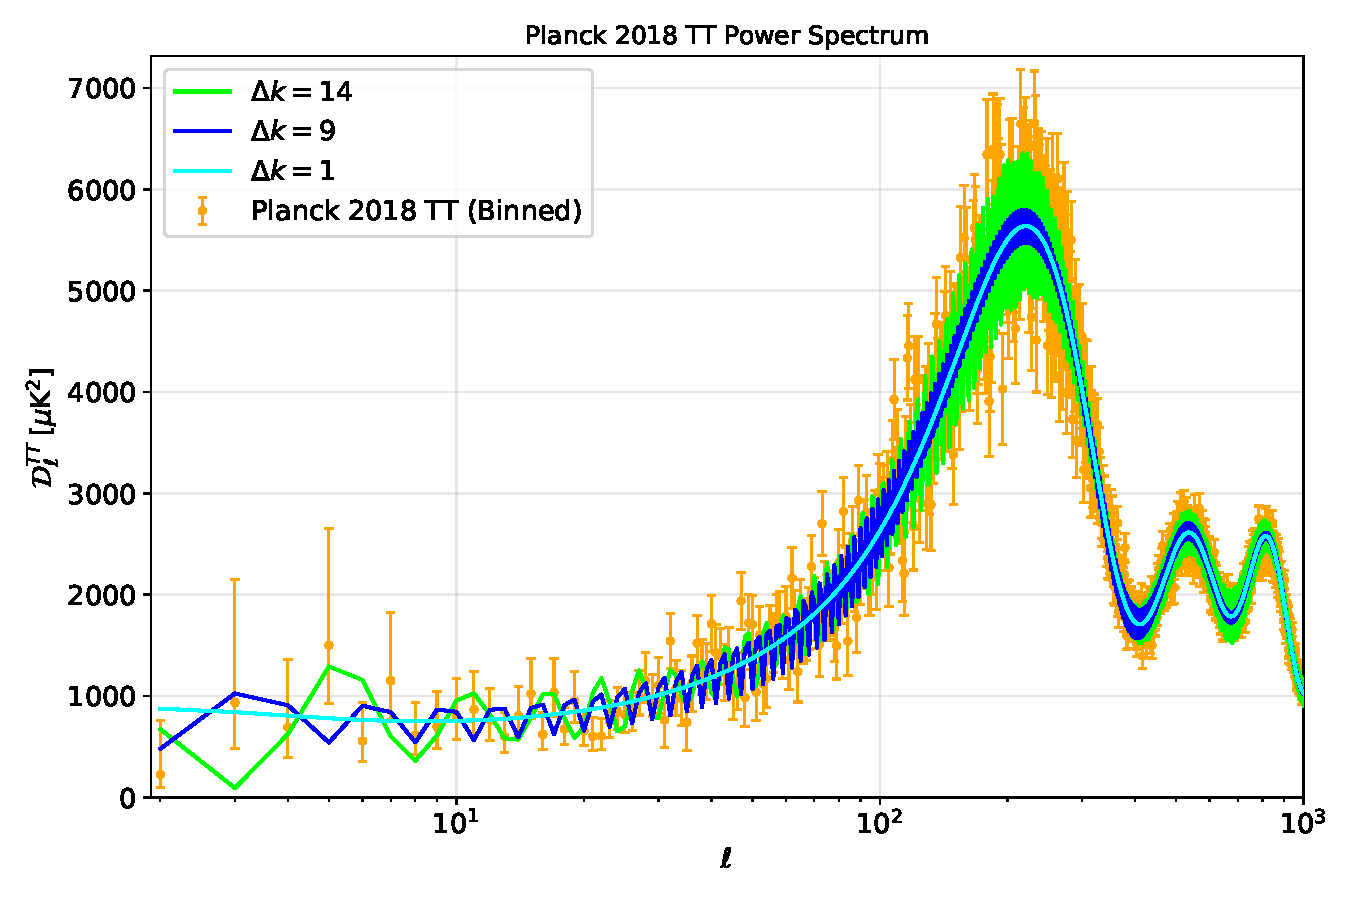
\includegraphics[width=0.85\textwidth]{./parts/part1/figures/CMB_diff_nuspacing.pdf}
     \centering
     \caption{The CMB temperature power spectrum calculated for different effective fundamental mode spacings, characterized by $\Delta k = N$. Here, $N=1$ corresponds to the standard closed $\Lambda$CDM model. For this illustrative plot, we fix $\Omega_K$ and other cosmological parameters to be Planck best-fit values, and isolate the effect of the mode spacing. Larger values of $N$ (a sparser sampling in $k$-space) lead to more fluctuations on large angular scales.}
     \label{fig:CMB_diffN}
\end{figure*}

\subsection{Post-processing \texttt{Planck 2018} MCMC Samples}\label{subsec:compare_planck}

Given that the discreteness features are not expected to be prominent, we can employ an efficient method to constrain our model's parameters without performing a full, computationally expensive Markov Chain Monte Carlo (MCMC) analysis. Instead of fitting our modified \texttt{CLASS} code directly to the data, we post-process the publicly available \texttt{Planck 2018} MCMC chains from the standard $\Lambda$CDM+$\Omega_K$ analysis (\texttt{base\_omegak\_plikHM\_TTTEEE\_lowl\_lowE}). This approach is valid because the likelihood surface of the standard model serves as a good approximation for our model.

Our procedure is as follows: for each sample point in the Planck MCMC chain, we use its cosmological parameters ($\Omega_m, \Omega_K, \Omega_b, h$, etc.) to calculate $\Delta k \equiv \Delta\tilde{k}(\tilde{m}, \tilde{\kappa}, \Omega_b, h) / \sqrt{\tilde{\kappa}}$. We then filter the chains, retaining only those samples for which this calculated value is approximately equal $\pm 2\%$ to an integer $N$. This filtering process isolates the regions of the standard model's posterior distribution that are consistent with our theoretical constraint. These filtered subsamples are then used to construct the marginalized posterior distributions for each allowed integer $N$, which we visualize using \texttt{anesthetic} \cite{anesthetic}.

\section{Results and Discussion}\label{sec:result}

\Cref{fig:perturbations_allowedK} displays the numerical solutions for several allowed perturbation modes. As theoretically expected, these solutions exhibit total symmetry or antisymmetry at the future conformal boundary. The solutions are generated using the best-fit cosmological parameters for the $\Delta k=4$ case, a choice we justify later as being favored by \texttt{Planck 2018} data \cref{fig:omegak_vs_chi2}.

% The figure environment from your original code
\begin{figure*}
     \centering % Good practice to center the figure
     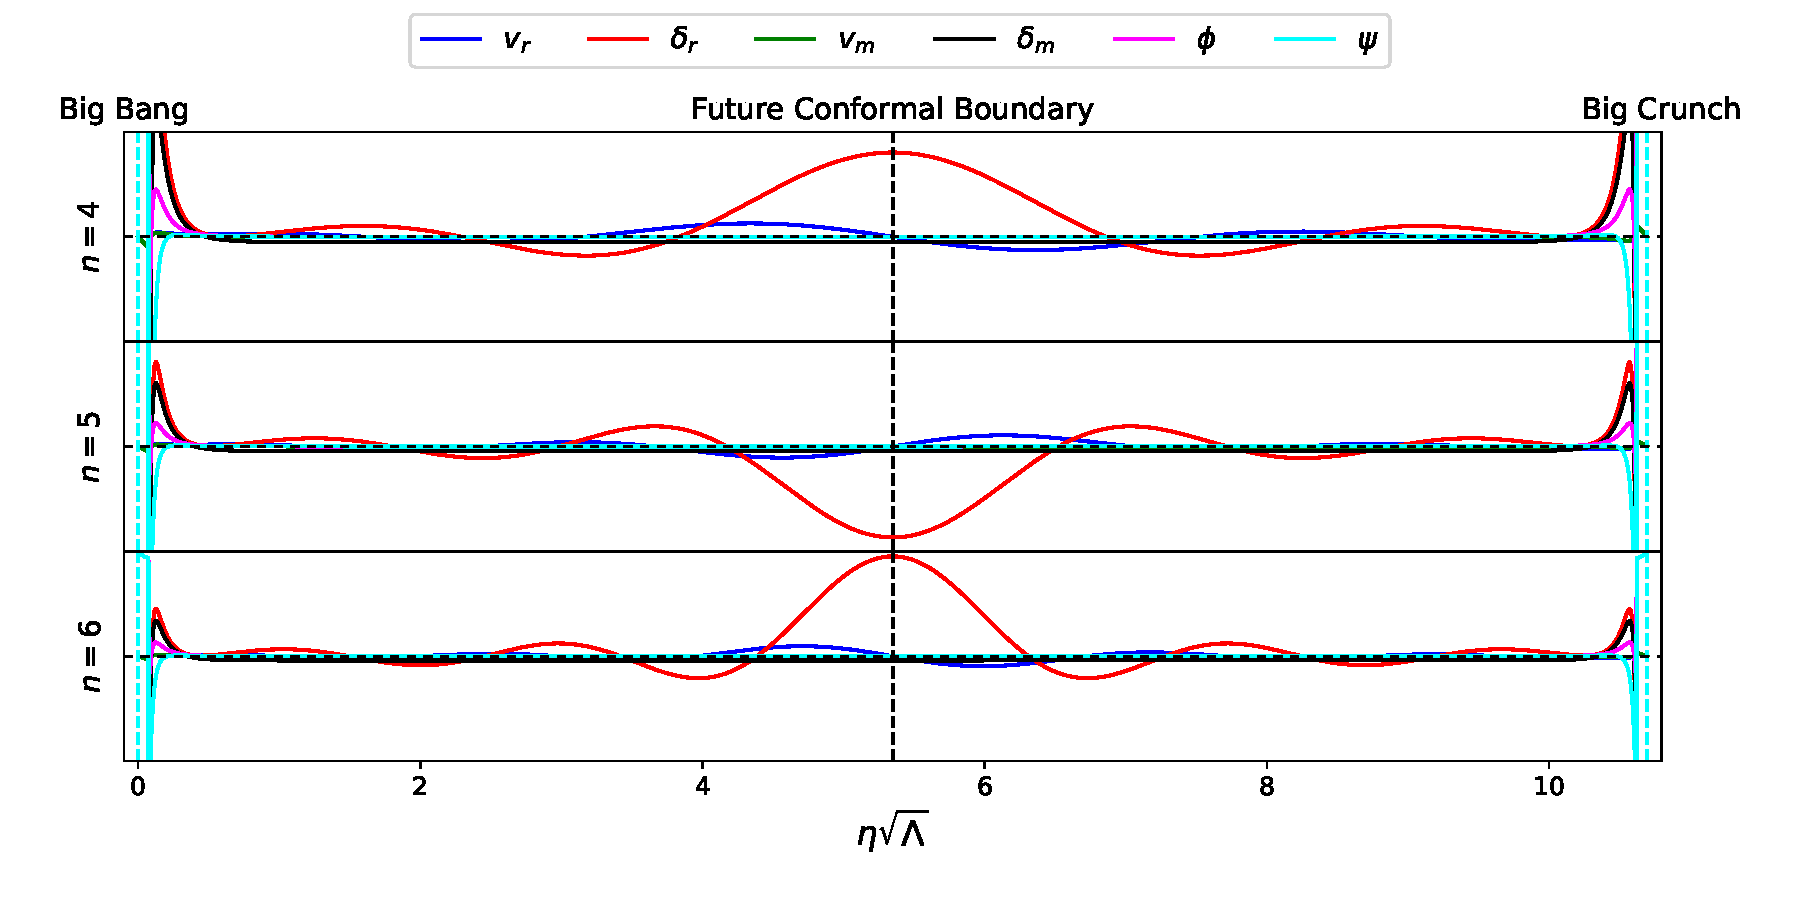
\includegraphics[width=\textwidth]{./parts/part1/figures/perturbation_solutions_allowedK.pdf}
     \caption{Numerical solutions for several allowed perturbation modes (modes 4--6 are shown to clarify the oscillatory behavior). As expected, the solutions are totally symmetric or antisymmetric at the future conformal boundary. The plot uses best-fit parameters corresponding to the $\Delta k=4$ case: $\Omega_m=0.435, \Omega_K=-0.038, h=0.564, \Omega_b=0.072$.}
     \label{fig:perturbations_allowedK}
\end{figure*}

These perturbation solutions are a crucial input for our analysis. Specifically, they are used to compute the function $\Delta\tilde k(\tilde m, \tilde \kappa, \Omega_b, h)$, which in turn allows us to filter the \texttt{Planck 2018} MCMC data samples by selecting only those that satisfy the theoretical constraint $\Delta \tilde k/\sqrt{\tilde{\kappa}}=N$. The outcome of this filtering process, which constitutes the primary result of our analysis, is shown in \cref{fig:Planck_diffN}. This figure presents the marginalized posterior distributions derived from the constrained MCMC samples. The full posterior for the standard $\Lambda$CDM+$\Omega_K$ model is shown in orange, while the colored contours highlight the subsets of samples that satisfy our consistency condition, $\Delta k \approx N$, for different integer values of $N$. The plot clearly demonstrates that our theoretical framework restricts the allowed parameter space to a series of discrete "islands," most prominently visible in the posterior for the spatial curvature parameter, $\Omega_K$. This corresponds to a discrete set of allowed values for the spatial curvature, with the most favored values being $\Omega_K \in [-0.076,-0.039, -0.024, -0.016, -0.012, \dots]$ for $N=3,4, 5, 6, 7, \dots$, respectively.

As predicted by our theoretical considerations in \cref{subsec:modify_CLASS}, the results show a distinct inverse relationship between the integer $N$ and the magnitude of the spatial curvature $|\Omega_K|$. Larger values of $N$ correspond to solutions that are closer to a spatially flat universe. This is a direct consequence of the constraint $\Delta\tilde{k} = N\sqrt{\tilde{\kappa}}$ coupled with the relative stability of the calculated $\Delta\tilde{k}$ across the parameter space. 

\begin{figure*}
     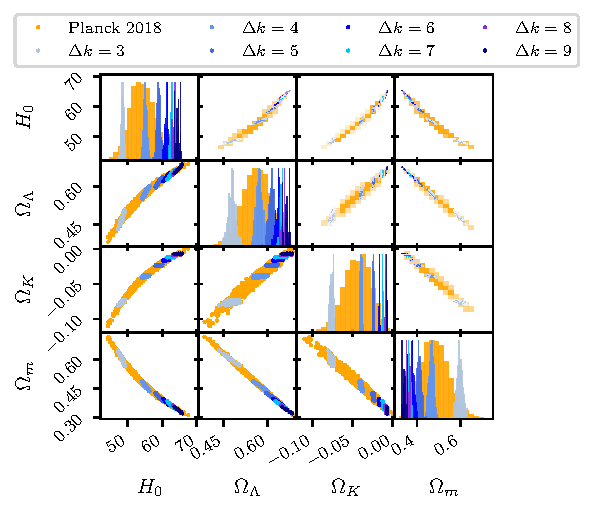
\includegraphics[width=0.9\textwidth]{./parts/part1/figures/Planck_TrianglePlot_diffDeltaK.pdf}
     \caption{Marginalized posterior distributions from \texttt{Planck 2018} MCMC samples for the \texttt{base\_omegak\_plikHM\_TTTEEE\_lowl\_lowE} likelihood combination. The orange contours represent the full posterior for the standard $\Lambda$CDM+$\Omega_K$ model. The colored regions highlight the subsets of samples that satisfy our consistency constraint $\Delta k \approx N$ for various integers $N$.}
     \label{fig:Planck_diffN}
\end{figure*}

To determine which of these discrete parameters is most favored by the data, we examine the $\chi^2$ value for each family of parameters. \cref{fig:omegak_vs_chi2} plots $\Delta\chi^2$ against $\Omega_K$ for the filtered samples. The analysis reveals a clear minimum at $N=4$, indicating that this is the most probable solution according to the \texttt{Planck 2018} data alone. 

\begin{figure}
     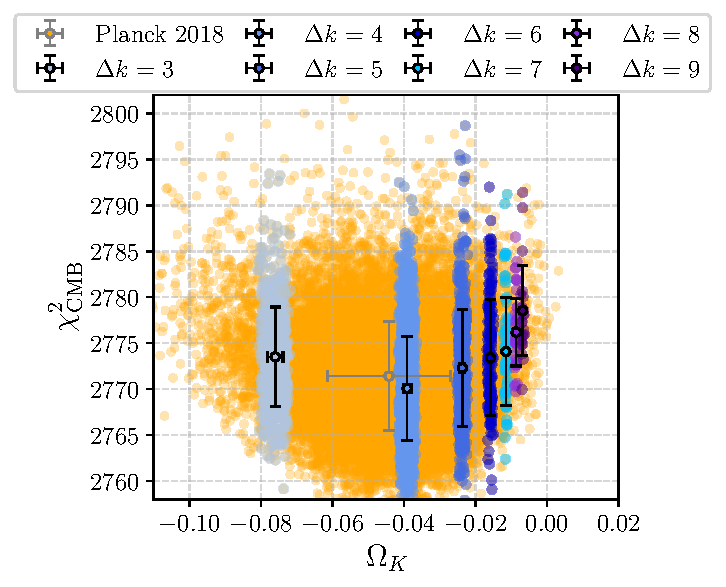
\includegraphics[width=0.7\textwidth]{./parts/part1/figures/Planck_omegak_vs_chi2.pdf}
     \centering
     \caption{A scatter plot of $\Delta\chi^2$ versus $\Omega_K$ for the filtered MCMC samples. The points show the mean value and $1\sigma$ error bars for each integer solution $\Delta k=N$. The minimum $\Delta\chi^2$ occurs for $N=4$, indicating it is the solution most favored by the \texttt{Planck 2018} data.}
     \label{fig:omegak_vs_chi2}
\end{figure}

It is important to discuss the cosmological parameters associated with the best-fit solution ($N=4$). The preferred values, such as $\Omega_m =0.467^{+0.012}_{-0.013}$ and $H_0 = 55.045^{+0.518}_{-0.485}$ km s$^{-1}$Mpc$^{-1}$, are different from the values derived from a flat $\Lambda$CDM cosmology and other cosmological probes. This discrepancy is a well-known consequence of the strong degeneracy within the CMB data: a wide range of parameter combinations, particularly involving $\Omega_K$, $\Omega_m$, and $H_0$, can produce nearly identical CMB power spectra.

To break this degeneracy and robustly test our model, it is necessary to perform a joint analysis with other cosmological datasets, such as Baryon Acoustic Oscillations (BAO) and Type Ia Supernovae (SNIa). However, such an analysis requires careful consideration of underlying assumptions. Many BAO analyses, for instance, assume a fiducial flat cosmology, which can inadvertently bias the results against a curved universe. A rigorous test demands that spatial curvature be treated as a free parameter consistently across all datasets. Indeed, analyses that do so, such as the work by Glanville et al. \cite{2022MNRAS.517.3087G} on BAO data, have also shown a preference for a closed universe. A comprehensive joint analysis, which we defer to future work, will therefore be crucial for discriminating between the allowed integer solutions and determining the true quantized value of spatial curvature.

\section*{Data Availability Statement}
The source code and data used for generating all figures and results in this study is publicly available in the GitHub repository \cite{code_for_figures_2509.10379} and Zenodo \cite{code_for_figures_2509}.

\begin{subappendices}
\section{Taylor Expansion Coefficients}\label{sec:Taylor}
To determine the cosmological perturbation solutions at the end of the universe, denoted by $\mathbf{X}^\infty$, we employ a Taylor expansion. For this purpose, it is advantageous to re-express the governing perturbation equations in terms of the reciprocal scale factor, $s \equiv 1/a$. This is because the end of the universe (where the scale factor $a \to \infty$) corresponds to $s \to 0$, a limit around which the coefficients of the differential equations behave well, allowing for a systematic expansion. The solutions at $s=0$ (conformal time $\eta_\infty$) are then extrapolated from solutions at a slightly earlier conformal time $\eta' = \eta_\infty - \Delta\eta$, where $\Delta\eta$ is a small, positive interval and serves as the expansion parameter. The relationship between the solutions at $\eta'$ and $\mathbf{X}^\infty$ is given by:
\begin{equation}\label{eq:taylor_relation}
\begin{pmatrix}
\mathbf{x}' \\
\mathbf{y}'_{2:4}
\end{pmatrix}
=
\begin{pmatrix}
\mathbf{X}_1 \\
\mathbf{X}_2
\end{pmatrix}
\mathbf{X}^\infty
\end{equation}
Here, $\mathbf{X}^\infty$ represents the vector of perturbation modes at $\eta_\infty$ (note that $\phi^\infty=\psi^\infty=0$)
\begin{equation}\label{eq:X_infty_def}
    \mathbf{X}^\infty = (\delta_r^\infty, \delta_m^\infty, v_r^\infty, \dot{v}_m^\infty)^T.
\end{equation}
The vectors $\mathbf{x}'$ and $\mathbf{y}'_{2:4}$ contain the perturbation variables at $\eta'$:
\begin{equation}\label{eq:xy_prime_def}
\begin{aligned}
    \mathbf{x}' &= (\phi', \psi', \delta_r', \delta_m', v_r', v_m')^T, \\
    \mathbf{y}'_{2:4} &= (F_{r2}', F_{r3}')^T,
\end{aligned}
\end{equation}

The matrices $\mathbf{X}_1$ and $\mathbf{X}_2$ contain the Taylor expansion coefficients.

The coefficients within these matrices depend on various cosmological parameters and the wavenumber $k$. We define the following dimensionless combinations. 
\begin{equation}\label{eq:coeffs_c}
c_1 = \frac{H_{\infty}^3 \Omega_m}{s_0^3 \Omega_{\Lambda}}, \qquad
c_2 = \frac{H_{\infty}^4 \Omega_r}{s_0^4 \Omega_{\Lambda}}, \qquad
c_3 = \frac{H_{\infty}^2 \Omega_K}{s_0^2 \Omega_{\Lambda}},
\end{equation}
and a recurring denominator term:
\begin{equation}\label{eq:coeff_Kc}
\mathcal{K}_c = k^2 + 3c_3.
\end{equation}

For brevity in presenting $\mathbf{X}_1$, we define the following intermediate expressions:
\begin{align}\label{eq:ABCD_defs}
    A &= \frac{6k^6+26k^4c_3+288c_2c_3+12k^2(2c_3^2-7c_2)}{45\mathcal{K}_c}, \\
    B &= \frac{c_1}{\mathcal{K}_c} \left( -\frac{9}{2}\Delta\eta + \frac{2k^2-3c_3}{4}(\Delta\eta)^3 \right), \\
    C &= \frac{c_1}{\mathcal{K}_c} \left( -\frac{27}{2}\Delta\eta - \frac{3(k^2+12c_3)}{4}(\Delta\eta)^3 \right), \\
    D &= \frac{3k^2+4c_3}{120}.
\end{align}
The matrix $\mathbf{X}_1$ is then given by:
\begin{equation}\label{eq:X1_matrix_full}
\resizebox{\textwidth}{!}{$\displaystyle
\mathbf{X}_1=
\begin{pmatrix}
0 &
\frac{c_1}{\mathcal{K}_c} \left( -\frac{3}{2}\Delta\eta - \frac{c_3}{4}(\Delta\eta)^3 \right) &
\frac{c_2}{\mathcal{K}_c} \left( 6\Delta\eta + \frac{k^2+8c_3}{5}(\Delta\eta)^3 \right) &
\frac{c_1}{\mathcal{K}_c} \left( -\frac{9}{2}\Delta\eta - \frac{3(k^2+4c_3)}{4}(\Delta\eta)^3 \right) \\
% Row 2
0 &
\frac{c_1}{\mathcal{K}_c} \left( -\frac{3}{2}\Delta\eta - \frac{c_3}{4}(\Delta\eta)^3 \right) &
\frac{c_2}{\mathcal{K}_c} \left( 6\Delta\eta + \frac{k^2+8c_3}{5}(\Delta\eta)^3 \right) &
\frac{c_1}{\mathcal{K}_c} \left( -\frac{9}{2}\Delta\eta - \frac{3(k^2+4c_3)}{4}(\Delta\eta)^3 \right) \\
% Row 3
1 - \frac{1}{6}k^2 (\Delta\eta)^2 &
\frac{c_1}{\mathcal{K}_c} \left( -6\Delta\eta - \frac{3c_3-2k^2}{3}(\Delta\eta)^3 \right) &
-\frac{4k^4+12k^2c_3-72c_2}{3\mathcal{K}_c}\Delta\eta + A(\Delta\eta)^3 &
\frac{c_1}{\mathcal{K}_c} \left( -18\Delta\eta - (k^2+12c_3)(\Delta\eta)^3 \right) \\
% Row 4
0 &
1 + B &
\frac{c_2}{\mathcal{K}_c} \left( 18\Delta\eta + \frac{24c_3-7k^2}{5}(\Delta\eta)^3 \right) &
\frac{1}{2}k^2(\Delta\eta)^2 + C \\
% Row 5
\frac{1}{4}\Delta\eta - D(\Delta\eta)^3 &
-\frac{3c_1}{2\mathcal{K}_c}(\Delta\eta)^2 &
1 - \frac{3k^4+13k^2c_3+12(c_3^2-5c_2)}{10\mathcal{K}_c}(\Delta\eta)^2 &
-\frac{9c_1}{2\mathcal{K}_c}(\Delta\eta)^2 \\
% Row 6
0 &
-\frac{3c_1}{2\mathcal{K}_c}(\Delta\eta)^2 &
\frac{6c_2}{\mathcal{K}_c}(\Delta\eta)^2 &
-\Delta\eta - \frac{9c_1}{2\mathcal{K}_c}(\Delta\eta)^2 - \frac{c_3}{6}(\Delta\eta)^3
\end{pmatrix};
$}
\end{equation}
The matrix $\mathbf{X}_2$ is given by:
\begin{equation}\label{eq:X2_matrix_full}
\resizebox{\textwidth}{!}{$\displaystyle
\mathbf{X}_2 =
\begin{pmatrix}
\frac{1}{15}k^2(\Delta\eta)^2 - \frac{k^2(15k^2+14c_3)}{3150}(\Delta\eta)^4 &
-\frac{4k^2c_1}{15\mathcal{K}_c}(\Delta\eta)^3 &
\frac{8}{15}k^2\Delta\eta - \frac{4k^2(30k^4+118k^2c_3+84(c_3^2-5c_2))}{1575\mathcal{K}_c}(\Delta\eta)^3 &
-\frac{4c_1k^2}{5\mathcal{K}_c}(\Delta\eta)^3 \\
% Row 2
-\frac{1}{105}k^3(\Delta\eta)^3 &
\frac{k^3c_1}{35\mathcal{K}_c}(\Delta\eta)^4 &
-\frac{4}{35}k^3(\Delta\eta)^2 + \frac{k^3(30k^4+118k^2c_3+84(c_3^2-5c_2))}{3675\mathcal{K}_c}(\Delta\eta)^4 &
\frac{3k^3c_1}{35\mathcal{K}_c}(\Delta\eta)^4
\end{pmatrix}.
$}
\end{equation}


\end{subappendices}

\printbibliography[heading=subbibintoc, title={References for Chapter \thechapter}]
\chapter{Matching Spatial and Temporal Boundary Conditions in Low-$k$ Modes}\label{chapter:low-k}

\chapterabstract{
% Editor's note: Rewrote the abstract for clarity, flow, and conciseness.
In conformal time, the age of the universe becomes finite, and solutions to the Friedmann equations and cosmological perturbations exhibit periodicity. This temporal periodicity imposes boundary conditions that restrict allowed wave vectors to discrete values, which are generally inconsistent with those required by the spatial boundary conditions of a closed universe. This chapter identifies general linear combination solutions that simultaneously satisfy both spatial and temporal boundary conditions. The resulting mode mixing and omissions yield a primordial power spectrum (PPS) and a cosmic microwave background (CMB) power spectrum characterized by suppression and fluctuations at low $k$. These theoretical features have the potential to explain observed anomalies in \texttt{Planck} data.
}


% Introduction: perturbations in periodic universe -> discrete wave vectors -> low-k mode -> 1975 paper solution -> structure of the paper 

% 1. Mathematical Method, describe topological picture
% 2. Toy model, shows it works 
% 3. Cosmology 
% 4. Future work

\section{Introduction}

% Editor's note: Improved the flow of the opening paragraph. Rephrased awkward constructs like "till (physical) time goes to infinity" and "co-expand".

In \cref{chapter:theory}, we pointed out that the two distinct sets of discrete wave vectors--coming from temporal and spatial periodic BCs respectively--must be consistent with each other, providing a strong constraint on cosmological parameters. To facilitate comparisons with observations, we solved the perturbations numerically and derived precise constraint values for these parameters by comparing with \texttt{Planck 2018} data (in \cref{chapter:Observation}).

However, a hidden complexity remains in this framework. The two sets of discrete wave vectors can be matched because they are both equally spaced in the high-$k$ regime. The wave vectors derived from the spatial BC are equally spaced by definition ($\propto n\in\mathbb{N}$). In contrast, for the temporal BC, the discrete $k$ values become non-equally spaced in the low-$k$ regime, as the frequencies become sufficiently low that the effects of the finite temporal boundary condition can no longer be ignored. 

The goal of this chapter is to find \textbf{general} solutions that satisfy both sets of BCs simultaneously. We demonstrate that these solutions must be linear combinations of the basis functions corresponding to each individual BC. The coefficients for these linear combinations are determined by the eigenvectors of projection matrices, which are computed via the inner products of the two sets of basis functions. The structure of the chapter is as follows: First, we define the problem in \cref{sec:def_PDE}, explain the mathematical and geometric interpretation of our method in \cref{sec:linear_combine_solution}, and demonstrate its efficacy using a 2D toy model in \cref{sec:toy_model}. We then apply this methodology to cosmological perturbations in \cref{sec:real_cosmology_lowk}, and generate the primordial power spectrum (PPS) and cosmic microwave background (CMB) power spectrum from these solutions in \cref{sec:PPS_CMB}. Finally, we outline potential applications and avenues for future work in \cref{sec:future_work}. 

\section{Problem Formulation}\label{sec:def_PDE}

% Structure:
% 1. Define the PDE and its periodic BCs. 
% 2. Solve eigenvalue problem -> solution with discrete wave vectors. 
% 3. The bases with different BCs are miss-match -> change T or L to match them in high-k mode
% 4. If $m\neq 0$, miss-match in low-k modes.

Our original goal was to solve the perturbation equations within a closed, periodic universe. This problem can be intuitively simplified into a 2D toy model: standing waves $\Phi$ in a 1D cavity, which evolve periodically. In other words, the waves must be periodic in both the spatial and temporal directions. The solution is trivial for a massless field, $\partial_t^2\Phi - \partial_x^2\Phi=0$, which yields simple plane waves (see \cref{fig:plane_waves_x-t_contour}).

\begin{figure}
    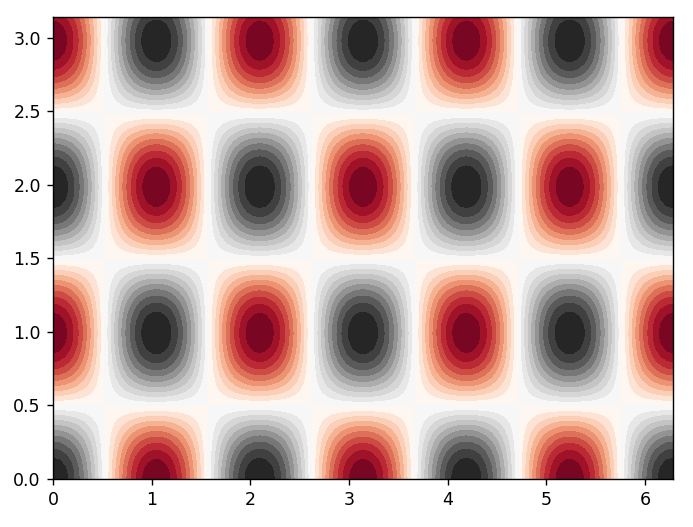
\includegraphics[width=0.5\textwidth]{parts/part1/figures/plane_waves_x-t_contour.png}
    \centering
    \caption{Contour plot of the plane wave $\Phi(x,t)=\exp(ikx)\cos(\omega t)$ in the $x-t$ plane, with wave vector $k=3$. The wave is periodic along both the $x$-axis and the $t$-axis.}
    \label{fig:plane_waves_x-t_contour}
\end{figure}

However, when generalized to a massive field, the situation becomes more complicated. To illustrate the problem, let us attempt to solve the Klein-Gordon equation:
\begin{equation}\label{eq:PDE}
    \partial_t^2\Phi - \partial_x^2\Phi + \mu^2\Phi = 0,
\end{equation}
where \(\mu\) represents the mass of the particle.
Following the separation of variables, \(\Phi(x,t) = \chi(x)\psi(t)\), the equation decouples into two eigenvalue problems:
\begin{equation}
    \partial_x^2\chi = -k^2\chi, \quad  
    \partial_t^2\psi = -\omega^2\psi,
\end{equation}
with the eigenvalues related by the dispersion relation \(\omega^2 = k^2 + \mu^2\).

To satisfy the periodic spatial and temporal BCs, the eigenvalues must be strictly discrete:
\begin{equation}
    k = n\frac{2\pi}{L}, \quad \omega = m\frac{2\pi}{T}, \quad n,m\in\mathbb{N},
\end{equation}
where \(L\) is the length of the spatial cavity, and \(T\) is the temporal period.

For any non-zero mass $\mu$, however, these independently discretized $k$ and $\omega$ values generally fail to satisfy the required relation \(\omega^2 = k^2 + \mu^2\). To resolve this, we first consider the high-frequency limit where \(\omega, k \gg \mu\), leading to \(\omega^2 \approx k^2\). This approximation can be satisfied by choosing a temporal period $T = N^{\pm1}L $, an approach analogous to the one utilized in our previous studies \cite{PhysRevD.110.103528, pjz6-47jv}. 

Despite this high-frequency alignment, a significant mismatch persists at low frequencies. Addressing this low-frequency discrepancy is the primary focus of this chapter and will be explored in the subsequent sections.

\section{Linear Combination Solutions}\label{sec:linear_combine_solution}

% Structure:
% 1. Idea: the solution should be linear combination of both bases.
% 2. Derivation -> the linear combination coefficients should be the eigenvectors with eigenvalue 1.
% 3. SVD and Physical picture: projection.

To resolve the mismatch problem, we propose constructing a linear combination of two distinct sets of bases that independently satisfy either the spatial or the temporal BCs:
\begin{equation}
    \phi_n = \chi_n(x)\psi_n(t), \quad \tilde\phi_m = \tilde\chi_m(x)\tilde\psi_m(t),
\end{equation}
where
\begin{equation}
\begin{aligned}
    k = n\frac{2\pi}{L}, \qquad \omega = \sqrt{k^2 + \mu^2}, \qquad n \in \mathbb{N}, \\
    \tilde\omega = m\frac{2\pi}{T}, \qquad \tilde{k} = \sqrt{\tilde{\omega}^2 - \mu^2}, \qquad m \in \mathbb{N}.
\end{aligned}
\end{equation}

The general solution can therefore be expressed equivalently in either basis:
\begin{equation}\label{eq:linear_combination}
    \Phi(x,t) = \sum_{n=1}^\infty c_n \phi_n = \sum_{m=1}^\infty \tilde{c}_m \tilde{\phi}_m.
\end{equation}

The primary objective is to determine the optimal linear combination coefficients, \(c_n\) and \(\tilde{c}_m\). This can be formulated as a linear algebra problem, specifically solved using algorithms designed to compute the "Principal Angles Between Subspaces" (such as the Björck-Golub algorithm \cite{1973MaCom..27..579B}). As it might not be familiar to the reader, we go through step-by-step derivation \cref{subsec:basic_derivation}, reinterpret in singular value decomposition (SVD) \cref{subsec:svd}, and finally provide a geometrical picture in 2D vector space \cref{subsec:geometric_view}. 

\subsection{Fundamental Derivation}\label{subsec:basic_derivation}

To determine these mixing coefficients, \(c_n\) and \(\tilde{c}_m\), we analogously apply finite-dimensional linear algebra. Given a vector \(\vec{v}\) in an \(N\)-dimensional space and an orthonormal basis \(\{ \vec{e}_i \}_{i=1}^N\), the vector's components are uniquely extracted via geometric projection:
\begin{equation}
    \vec{v} = \sum_{i=1}^N c_i \vec{e}_i, \qquad c_i = \vec{v} \cdot \vec{e}_i.
\end{equation}

Extending this formalism to a continuous function space, we truncate our two bases to \(N\) modes: \(\{ \phi_n(x,t) \}_{n=1}^N\) and \(\{ \tilde\phi_m(x,t) \}_{m=1}^N\). While these initial bases are not strictly mutually orthonormal, they can be systematically orthonormalized via the Gram-Schmidt process. To facilitate this, we define the standard inner product on the spacetime domain:
\begin{equation}
    f \cdot g = \int_0^T\int_0^L  f^*(x,t) g(x,t) \, dx \, dt.
\end{equation}

This inner product allows us to systematically project functions between the two bases, facilitating both orthonormalization and the extraction of the linear combination coefficients. 

Assuming the bases have been properly normalized to \(\varphi_n\) and \(\tilde\varphi_m\), projecting the target solution \(\Phi\) onto each yields the following coupled relations:
\begin{equation}\label{eq:coefficients_relation1}
\begin{aligned}
    c_n = \varphi_n \cdot \Phi = \varphi_n \cdot \left(\sum_{m=1}^N \tilde{c}_m \tilde{\varphi}_m\right) = \sum_{m=1}^N \tilde{c}_m (\varphi_n \cdot \tilde{\varphi}_m), \\
    \tilde{c}_m = \tilde{\varphi}_m \cdot \Phi = \tilde{\varphi}_m \cdot \left(\sum_{n=1}^N c_n \varphi_n\right) = \sum_{n=1}^N c_n (\tilde{\varphi}_m \cdot \varphi_n).
\end{aligned}
\end{equation}

By mutually substituting the expressions for \(\tilde{c}_m\) and \(c_n\) into one another, we obtain a closed-form eigenvalue problem:
\begin{equation}\label{eq:coefficients_relation2}
\begin{aligned}
    c_n &= \sum_{m=1}^N \sum_{n'=1}^N c_{n'} (\tilde{\varphi}_m \cdot \varphi_{n'}) (\varphi_n \cdot \tilde{\varphi}_m) = \sum_{n'=1}^N A_{nn'} c_{n'}, \\
    \tilde{c}_m &= \sum_{n=1}^N \sum_{m'=1}^N \tilde{c}_{m'} (\varphi_n \cdot \tilde{\varphi}_{m'}) (\tilde{\varphi}_m \cdot \varphi_n) = \sum_{m'=1}^N \tilde{A}_{mm'} \tilde{c}_{m'},
\end{aligned}
\end{equation}
where the projection matrices \(A\) and \(\tilde{A}\) are explicitly defined as:
\begin{equation}
\begin{aligned}
    A_{nn'} &= \sum_{m=1}^N (\varphi_n \cdot \tilde{\varphi}_m)(\tilde{\varphi}_m \cdot \varphi_{n'}), \\
    \tilde{A}_{mm'} &= \sum_{n=1}^N (\tilde{\varphi}_m \cdot \varphi_n)(\varphi_n \cdot \tilde{\varphi}_{m'}).
\end{aligned}
\end{equation}

These matrices, \(A\) and \(\tilde{A}\), mathematically encode the back-and-forth projections between the two functional spaces. The physically valid solutions—those identical in both bases—correspond precisely to the eigenvectors of \(A\) and \(\tilde{A}\) that possess an eigenvalue of exactly $1$.


\subsection{Alternative Perspective: Singular Value Decomposition}\label{subsec:svd}

% Editor's note: Improved flow and clarified the geometric interpretation of the matrices.
This projection technique can be elegantly recast using Singular Value Decomposition (SVD). We define the mixing matrix between the two bases as \(M_{nm} = \varphi_n \cdot \tilde{\varphi}_m\), which decomposes factorially as \(M = U \Sigma V^\top\).

In this decomposition, the columns of \(U\) are the eigenvectors of \(MM^\top \equiv A\), which supply the optimal mixing coefficients for the \(\varphi_n\) basis. Similarly, the columns of \(V\) are the eigenvectors of \(M^\top M \equiv \tilde{A}\), supplying the coefficients for the \(\tilde{\varphi}_n\) basis. The non-zero elements of the diagonal matrix \(\Sigma\) are the singular values, equating to the square roots of the shared non-zero eigenvalues of \(A\) and \(\tilde{A}\).

Physically, this SVD approach isolates the invariant subspaces shared by the two overlapping bases. To make this geometric interpretation explicit, we define the bases as column vectors of functions:
\begin{equation}
\begin{aligned}
    |\varphi\big> = [\varphi_1, \varphi_2, \ldots, \varphi_N]^\top, \qquad |\tilde{\varphi}\big> = [\tilde{\varphi}_1, \tilde{\varphi}_2, \ldots, \tilde{\varphi}_N]^\top.
\end{aligned}
\end{equation}

Assuming there exist \(K\) numerically valid solutions (characterized by eigenvalues $\approx 1$), their corresponding \(N \times K\) coefficient matrices are written as:
\begin{equation}
\begin{aligned}
    C = [\vec{c}_1, \vec{c}_2, \dots, \vec{c}_K], \qquad \tilde{C} = [\vec{\tilde{c}}_1, \vec{\tilde{c}}_2, \dots, \vec{\tilde{c}}_K].
\end{aligned}
\end{equation}

The \(K\)-dimensional manifold of valid solutions can then be expressed globally as:
\begin{equation}
    |\Phi\big> = C^\top |\varphi\big> = \tilde{C}^\top |\tilde{\varphi}\big>.
\end{equation}

\cref{eq:coefficients_relation1} can then be recast in compact matrix notation as:
\begin{equation}
\begin{aligned}
    \begin{Bmatrix} 
        \tilde{C}^\top = |\Phi\big> \big< \tilde{\varphi}| = C^\top |\varphi\big> \big< \tilde{\varphi}| = C^\top M, \\
        C^\top = |\Phi\big> \big< \varphi| = \tilde{C}^\top |\tilde{\varphi}\big> \big< \varphi| = \tilde{C}^\top M^\top.
    \end{Bmatrix}
\end{aligned}
\end{equation}

Here, the mixing matrix \(M\) acts as a geometric mapping operator. It transforms the state coefficients from the \( |\varphi\big> \) basis directly into the \( |\tilde{\varphi}\big> \) basis, while its conjugate transpose \( M^\top \) strictly executes the inverse mapping.

For a solution \( |\Phi\big> \) to be globally valid, it must lie entirely within the intersection of the two basis subspaces. Consequently, its coefficient vectors must remain invariant under sequential back-and-forth projections between the \( |\varphi\big> \) and \( |\tilde{\varphi}\big> \) coordinate frames. This geometric invariance strictly requires that the coefficient matrices \(C\) and \(\tilde{C}\) be eigenvectors of \( MM^\top \) and \( M^\top M \), respectively, with an eigenvalue of $1$:
\begin{equation}
    \begin{Bmatrix}
    C = MM^\top C = AC, \\
    \tilde{C} = M^\top M \tilde{C} = \tilde{A} \tilde{C},
    \end{Bmatrix}
\end{equation}
which confirms the matrix-level equivalence with \cref{eq:coefficients_relation2}.

\subsection{Two-Dimensional Geometric Analogy}\label{subsec:geometric_view}

% Editor's note: Rephrased the geometric explanation for enhanced clarity and flow.
Imagine two vector bases, $|\phi_n\big>$ and $|\tilde\phi_m\big>$ for $n,m \in \{1,2\}$, each spanning its own 2D plane. Our objective is to find a vector $\Phi$ that can be expressed as a linear combination within both bases. Geometrically, this requires the vector $\Phi$ to lie exactly at the intersection of the two planes, as depicted in \cref{fig:geometry_solution}. 

To find this solution $\Phi$, we first normalize the two bases to yield $|\varphi_n\big>$ and $|\tilde\varphi_m\big>$. The vector $\Phi$ can then be written as \( \Phi = \vec{c} \cdot |\varphi\big> = \sum_{n=1}^N c_{n} \varphi_n \) and \( \Phi = \vec{\tilde{c}} \cdot |\tilde{\varphi}\big> = \sum_{m=1}^N \tilde{c}_{m} \tilde{\varphi}_m \). The algorithm relies on the projection matrix $M_{nm} = |\varphi_n\big>\big<  \tilde{\varphi}_m|$, which maps the coefficient vector from the \( |\varphi\big> \) plane onto the \( |\tilde{\varphi}\big> \) plane. The transpose, \( M^\top_{mn}=|\tilde\varphi_m\big>\big<  {\varphi}_n| \), performs the reverse projection. A valid solution $\Phi$ must remain invariant under this back-and-forth projection. Specifically, the coefficient vectors \( \vec{c} \) and \( \vec{\tilde{c}} \) must be eigenvectors of \( MM^\top \) and \( M^\top M \), respectively, each corresponding to an eigenvalue equal to $1$.

\begin{figure}[htbp]
    \centering
    % Left Subfigure
    \begin{subfigure}[t]{0.485\textwidth}
        \centering
        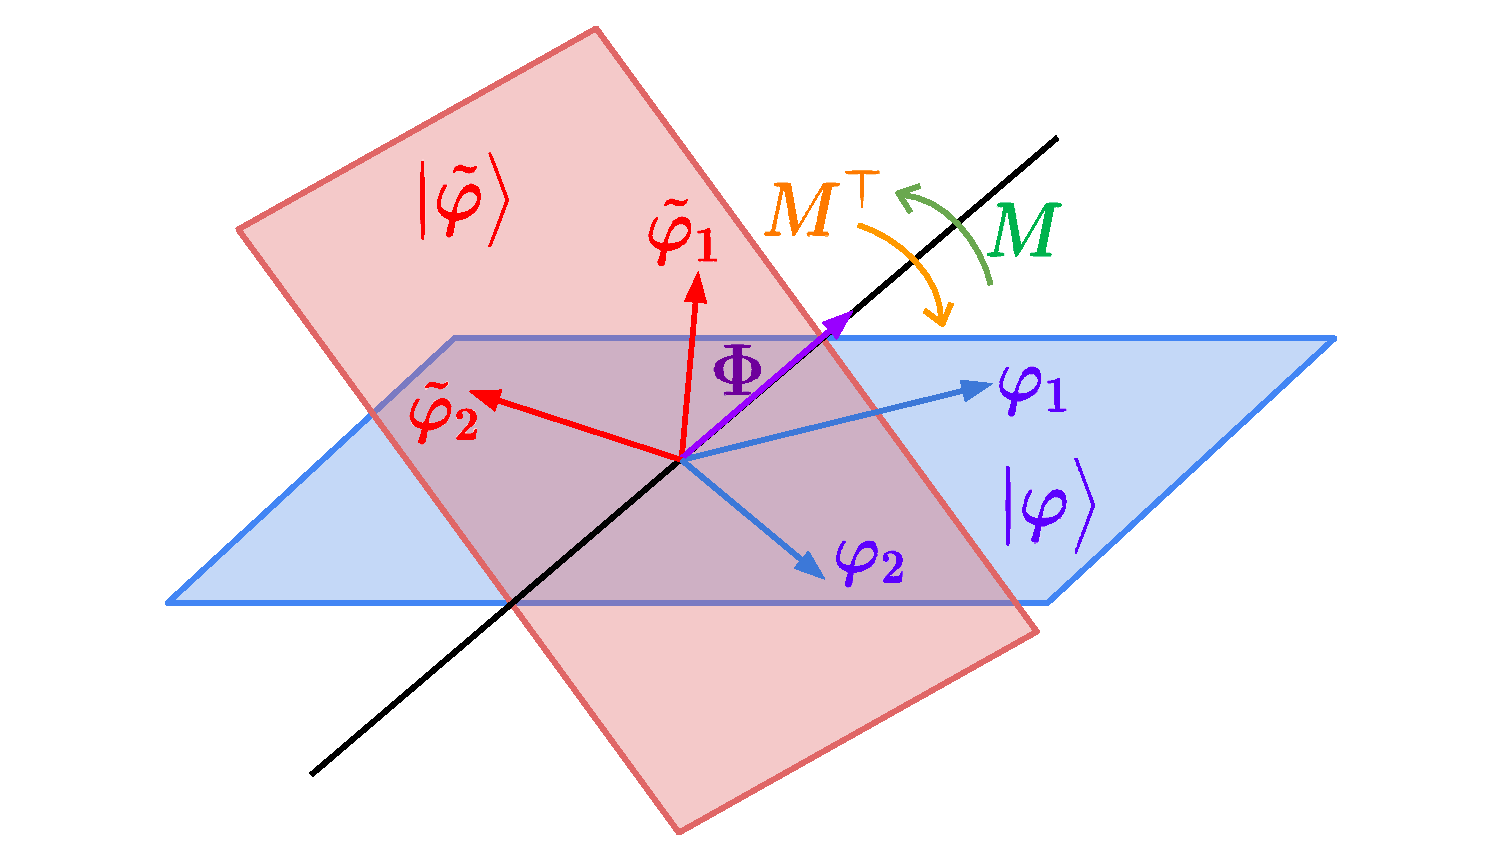
\includegraphics[width=\textwidth]{parts/part1/figures/geometry_solution.pdf}
            \caption{Geometric interpretation of the solution method. The solution vector \( \Phi \) lies at the intersection of two distinct planes, spanned by \( |\varphi\big> \) and \( |\tilde{\varphi}\big> \). The projection matrices \( M \) and \( M^\top \) map vectors between these planes. The eigenvectors of \( MM^\top \) and \( M^\top M \) provide the valid coefficients for the solution in each respective basis.}
        \label{fig:geometry_solution}
    \end{subfigure}%
    \hfill
    % Right Subfigure
    \begin{subfigure}[t]{0.485\textwidth}
        \centering
        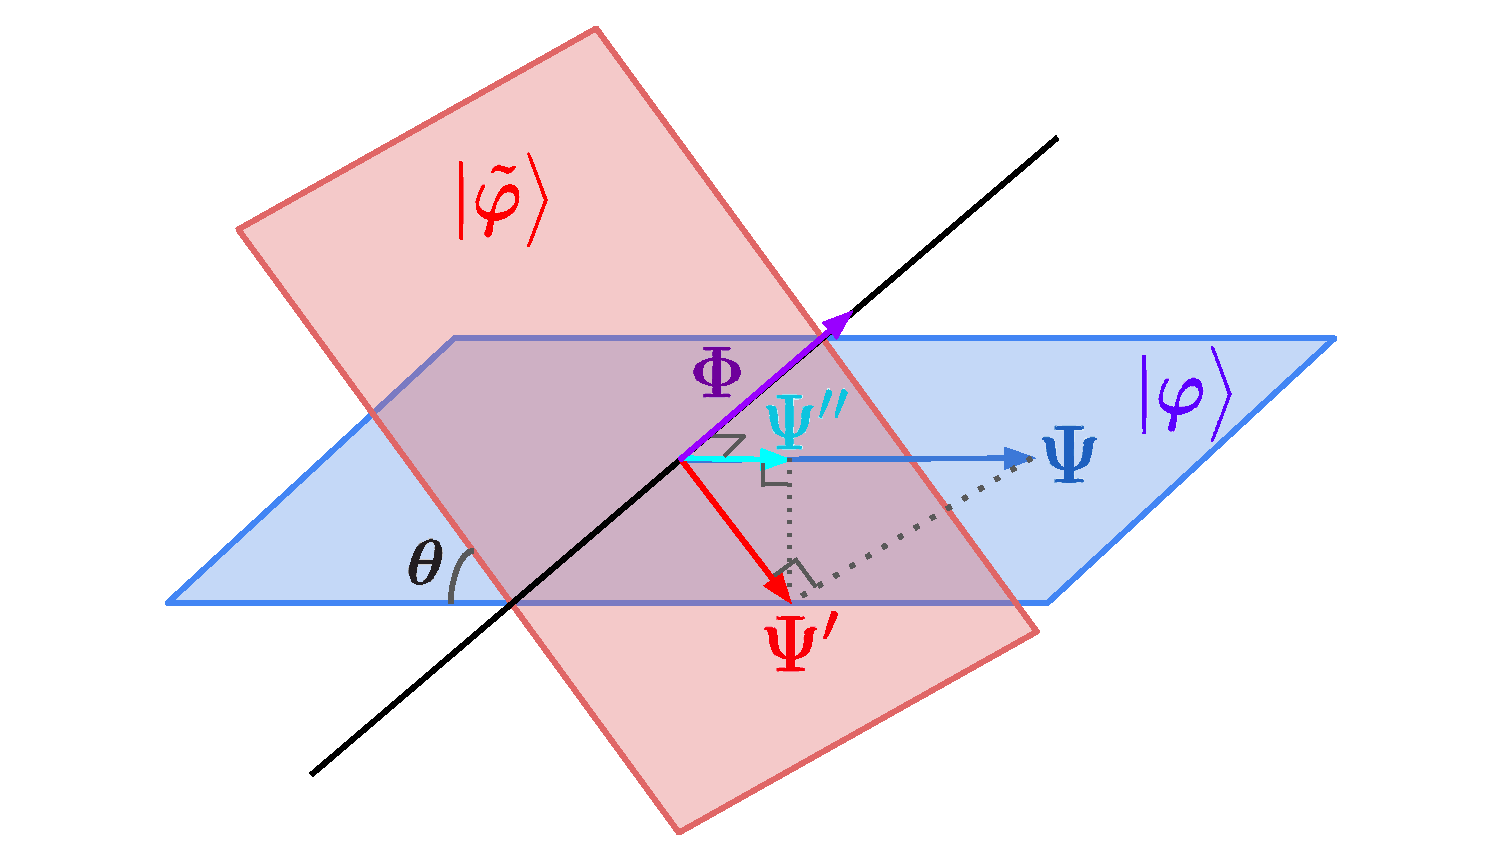
\includegraphics[width=\textwidth]{parts/part1/figures/geometry_non_solution.pdf}
        \caption{Geometric interpretation of the non-solution eigenvector \( \Psi \). Its magnitude is not conserved upon projection back and forth between the planes, resulting in an eigenvalue strictly less than $1$.}
        \label{fig:geometry_non_solution}
    \end{subfigure}
\end{figure}

In this 2D analogy, \( MM^\top \) possesses two eigenvectors, \( \vec{c}_1 \) and \( \vec{c}_2 \), which are orthogonal to one another. Assume $\vec{c}_1$ contains the coefficients that successfully construct the target solution $\Phi$. The second eigenvector, $\vec{c}_2$, constructs a different vector \( \Psi \), which initially lies entirely in the \( |\varphi\big> \) plane (see \cref{fig:geometry_non_solution}). When \( \Psi \) is projected onto the \( |\tilde{\varphi}\big> \) plane, only the component parallel to this new plane survives, yielding \( \Psi' = \cos(\theta) \Psi \), where \( \theta \) is the dihedral angle between the planes. Projecting \( \Psi' \) back onto the original \( |\varphi\big> \) plane produces \( \Psi'' = \cos^2(\theta) \Psi \). While the direction of \( \Psi \) is preserved, its magnitude is attenuated by a factor of \( \cos^2(\theta) \). Consequently, \( \vec{c}_2 \) is an eigenvector of \( MM^\top \) with an eigenvalue of \( \cos^2(\theta) \). As the angle between the planes decreases, the eigenvalue approaches $1$; conversely, if the planes are nearly orthogonal (\( \theta \approx \pi/2 \)), the eigenvalue approaches zero.


Since our goal is to find \( \Phi \), not \( \Psi \), we selectively isolate the eigenvectors of \( MM^\top \) and \( M^\top M \) that are associated with eigenvalues equal to $1$.

This geometric angle between the planes serves as an excellent analogy for the functional difference between the two bases in our wave equation, which is dictated by the parameters \( \mu \) and \( T \). If the mass \( \mu \) decreases and $T \approx N^{\pm1}L$, the discrepancy between the two bases diminishes. Geometrically, the planes become more aligned (smaller $\theta$), yielding a greater number of eigenvalues near $1$. 


\section{Results for the Toy Model}\label{sec:toy_model}

% Structure:
% 1. Details of the problem
% 2. Solution with \mu=0.5, T=\pi, L=2\pi, show the solution, x-t plot, cylinder plot, and the distribution of the coefficients
% 3. varies \mu, show the x-t plot and distribution of the coefficients
% 4. varies T, show the solutions

To ensure the two bases are consistent at high $k$ modes, we require $T = N^{\pm1}L $. For this demonstration, we choose $L=2\pi$ and $T=\pi$, utilizing Neumann initial conditions (ICs) for the perturbations. This ensures that the discrete $k$ values satisfying the spatial BCs are integers, and the solutions are either symmetric or anti-symmetric at both the Bang and the end of the universe, closely mimicking the temporal BCs required for perturbations in a periodic universe \cite{2022PhRvD.105h3514L}. The particle mass is set to $\mu = 0.1$ for the subsequent figures.

\cref{fig:coefficients_T3.14_m0.1} displays the linear combination coefficients for the first four solutions projected onto the basis \(|\phi\big>\). It is evident that each solution inherently requires a superposition of modes with varying frequencies.

\cref{fig:solution_T3.14_m0.1} illustrates the amplitude evolution over time for the four lowest-order solutions, measured at the spatial coordinate $x=\pi$. The time series reconstructed independently from the two bases are visually identical, validating our foundational assumption in \cref{eq:linear_combination} that a valid solution must be a convergent linear combination of both bases.


\begin{figure}
    % Editor's note: Removed the stray closing parenthesis in the caption/text reference for this figure.
    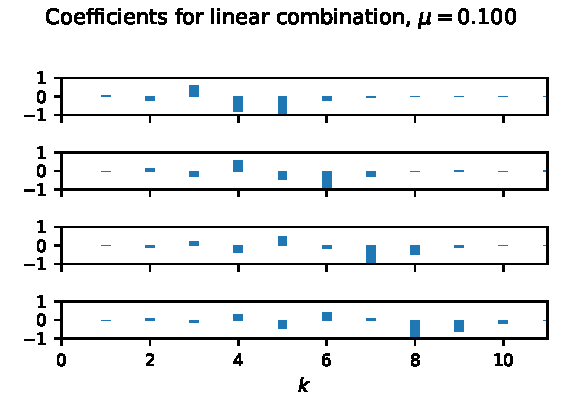
\includegraphics[width=0.7\textwidth]  {parts/part1/figures/eigenvalue_2d_N30_Nt150_T3.14_m0.100_coefficients.pdf}
    \centering
        \caption{The linear combination coefficients of the first four valid solutions, corresponding to the basis $|\phi\big>$, sorted by the frequency of their dominant mode. The coefficients are normalized to a maximum of $1$. The x-axis represents $k \in \mathbb{N}$, which are the strictly allowed wave vectors for the basis $|\phi\big>$.}
        \label{fig:coefficients_T3.14_m0.1}
\end{figure}

\begin{figure}
    % Editor's note: Removed the stray closing parenthesis in the caption/text reference for this figure.
    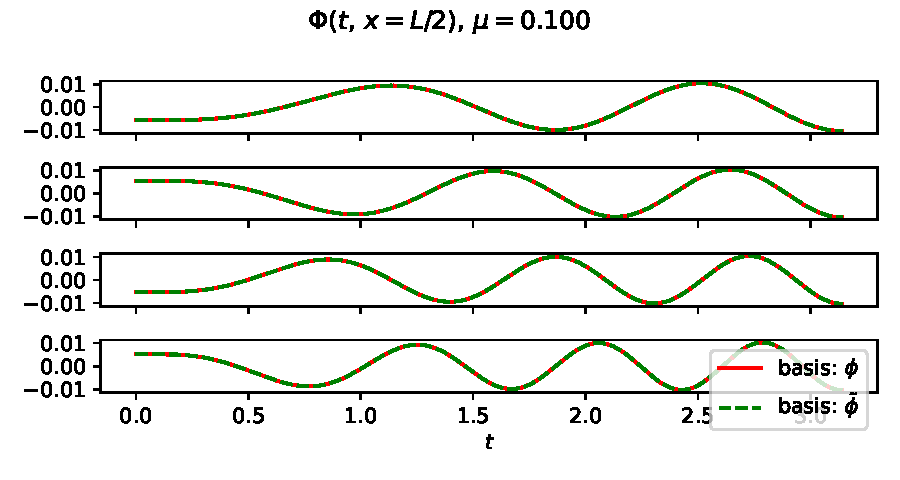
\includegraphics[width=0.8\textwidth]{parts/part1/figures/eigenvalue_2d_N30_Nt150_T3.14_m0.100_xpi.pdf}
    \centering
        \caption{Amplitude-time traces of the numerical solutions evaluated at \(x = \pi\). The red solid lines and the green dashed lines represent the solutions reconstructed using the bases \(|\phi\big>\) and \(|\tilde{\phi}\big>\), respectively.}
        \label{fig:solution_T3.14_m0.1}
\end{figure}


\cref{fig:contour_T3.14_m0.1} presents the corresponding contour plots in the \(x\)-\(t\) plane for these four solutions. The distinctive V-shaped interference patterns arise directly from the superposition of multiple wave frequencies. Specifically, combining simple plane-wave checkerboard patterns (see \cref{fig:plane_waves_x-t_contour}) with different frequencies naturally generates these V-shaped patterns.

\cref{fig:contour_cylinder_T3.14_m0.1} visualizes the solution exhibiting a dominant \(k=5\) mode wrapped onto a cylinder, akin to Fig.~2 in \cite{2021arXiv210906204B}. Here, the azimuthal \(x\)-\(y\) plane represents a closed spatial dimension, while the vertical \(z\)-axis corresponds to conformal time. This visually reinforces that the perturbation perfectly respects periodicity in both space and time.


\begin{figure}[htbp]
    \centering
    % Left Subfigure
    \begin{subfigure}[b]{0.58\textwidth}
        \centering
        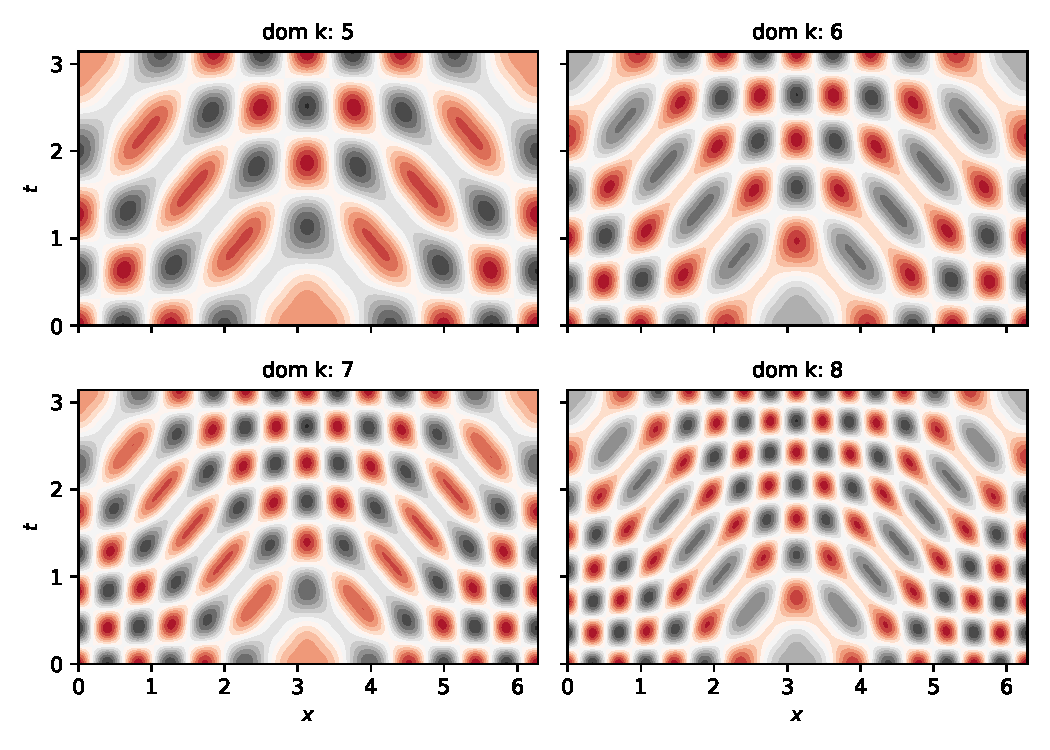
\includegraphics[width=\textwidth]{parts/part1/figures/eigenvalue_2d_N30_Nt150_T3.14_m0.100_contour_sequences.pdf}
        \caption{Spatiotemporal (\(x\)-\(t\)) contour plots for the first four fundamental solutions.}
        \label{fig:contour_T3.14_m0.1}
    \end{subfigure}%
    \hfill
    % Right Subfigure
    \begin{subfigure}[b]{0.39\textwidth}
        \centering
        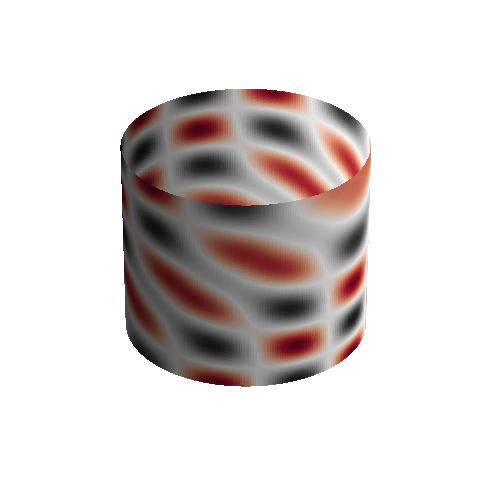
\includegraphics[width=\textwidth]{parts/part1/figures/eigenvalue_2d_N30_Nt150_T3.14_m0.100_cylinder_kdom5.pdf}
        \caption{Cylindrical projection of the solution with a dominant mode of \(k=5\). The azimuthal direction represents the closed spatial dimension, while the vertical axis maps to conformal time.}
        \label{fig:contour_cylinder_T3.14_m0.1}
    \end{subfigure}
\end{figure}

Finally, we consider the impact of varying the particle mass $\mu$. As previously noted, an increase in $\mu$ widens the discrepancy between the two bases, analogous to increasing the dihedral angle between the 2D planes in \cref{fig:geometry_solution}. Consequently, fewer eigenmodes possess eigenvalues sufficiently close to one, leading to an increased number of "missing" or forbidden modes in the low-$k$ regime. \cref{fig:dom_k_vs_m} shows the lowest dominant $k$ as a function of particle mass. It is clear that as the mass increases, the lowest permissible dominant mode is pushed toward larger values of $k$ due to these missing modes. Similarly, as eigenvalue threshold increases, more low-$k$ modes are omitted of their smaller eigenvalues.

\begin{figure}
    % Editor's note: Removed the stray closing parenthesis in the caption/text reference for this figure.
    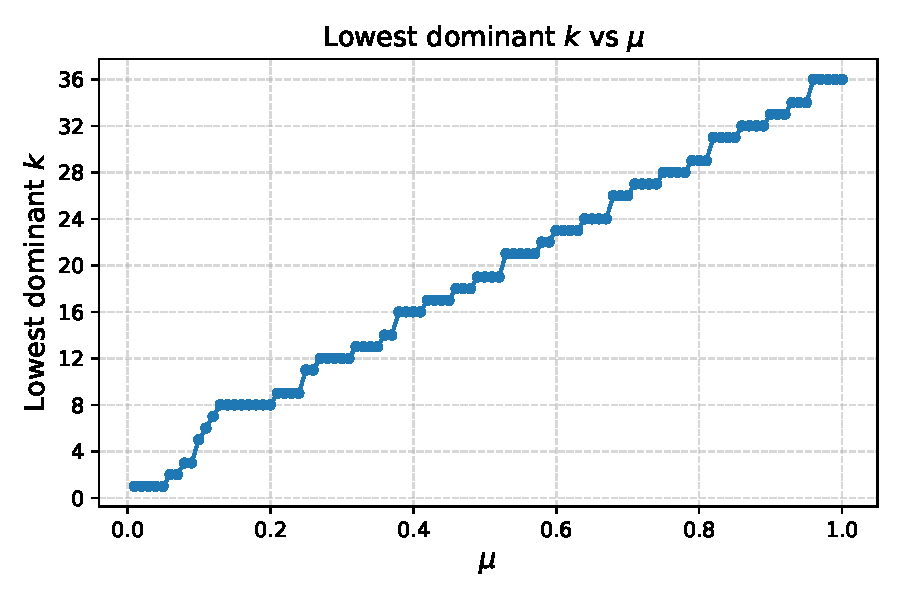
\includegraphics[width=0.7\textwidth]{parts/part1/figures/dom_k_vs_mu.pdf}
    \centering
    \caption{The lowest dominant mode across different particle masses. When mass increase, there would be more missing modes, pushing the lowest dominate $k$ to higher value. }
    \label{fig:dom_k_vs_m}
\end{figure}

\section{Applications to Cosmological Perturbations}\label{sec:real_cosmology_lowk}

We now apply this methodology to a cosmological perturbations. Several physical and numerical complexities must be addressed:

\begin{enumerate}
    \item \textbf{Cosmological Parameters:} Real cosmology introduces several parameters that dictate the expansion history. These parameters must be constrained not only by demanding consistency between the two bases, but also by ensuring alignment with observations.
    \item \textbf{Coupled Fields:} The toy model features only a single scalar field, whereas realistic cosmology requires multiple perturbation fields to be coupled together. A physically valid solution must ensure that all perturbation fields simultaneously match the BCs using a single set of shared linear combination coefficients.
    \item \textbf{Phenomenological Preference:} In the toy model, any arbitrary linear combination of valid eigen-solutions will still satisfy both BCs. However, in cosmology, certain bases (specifically, those approaching pure integer modes) are phenomenologically preferred when comparing predictions to standard observational expectations. 
\end{enumerate}

The strategies utilized to address each of these points are detailed in the following subsections.

\subsection{Determination of Cosmological Parameters}

In the toy Klein-Gordon equation, the sole background parameter is $T$ (time period), which must satisfy $T=N^{\pm 1}\pi$ (where $N\in\mathbb{N}$) to ensure the temporally allowed $k$ modes converge to integers at high-$k$. Similarly, in cosmology, multiple parameters ($\Omega_m, \Omega_K, \Omega_b, h$) must be jointly determined such that the conformal age of the universe satisfies $\eta_{\text{age}}= N^{\pm1}\sqrt{3}\pi$. Furthermore, observational data (e.g., the CMB power spectrum) impose stringent external constraints on these parameters. 

To determine the optimal cosmological parameters satisfying both conditions, we employ a three-step procedure: 
(1) We use a \texttt{KDTree} algorithm to interpolate the CMB likelihood surface $\chi^2(\Omega_m,\Omega_K,\Omega_b,h)$, identifying regions of parameter space that broadly fit observations. This prevents the wasteful execution of expensive ODE solvers on observationally excluded parameters. 
(2) We utilize \texttt{Optuna}, an efficient machine learning optimization framework, to precisely locate the parameter combinations that minimize the deviation of allowed $k$-modes from pure integers. 
(3) From the top 10 best-fit parameter sets, we select the one that yields the lowest $\Delta\chi^2$ against the \texttt{Planck 2018} dataset \footnote{This is achieved by filtering the \texttt{Planck 2018} MCMC samples to isolate those nearest to our candidate parameter sets, and subsequently extracting the corresponding $\Delta\chi^2$ values.}.

% Editor's note: Changed the syntax-breaking \fotnotesize command to a standard font-sizing group to ensure compilation while maintaining intended visual formatting.
{\footnotesize Note that for allowed-$k$ vectors to genuinely map to integers, both their spacing and their intercept must be integers. However, due to lingering theoretical and numerical challenges in obtaining a robust intercept prediction \footnote{To ensure a reliable intercept, our perturbation solver requires two major upgrades: (1) Recombination: The current code directly splices solutions from before and after recombination, rather than integrating continuously through the era. (2) Neutrino physics: Proper modeling requires full neutrino perturbations that transition dynamically from relativistic to non-relativistic states. Both upgrades demand a major rewrite of the perturbation equations and initialization logic.}, the current optimization solely penalizes deviations in the mode spacing, temporarily ignoring the intercept.}

The integer spacing loss function over the cosmological parameter space is illustrated in \cref{fig:loss_param_space}. A lower loss indicates that the allowed-$k$ modes exhibit a spacing closer to exact integers (which is fixed to $4$ in this framework). The red stars indicate our finally selected best-fit parameters: $\Omega_m=0.4445$, $\Omega_K=-0.0394$, $\Omega_b=0.0716$, and $h=0.5615$.

Several physical dependencies are evident in this parameter space. First, the loss function depends heavily on $\Omega_m$ and $\Omega_K$, as these parameters directly dictate the conformal age of the universe. The baryon density $\Omega_b$, plays a more minor role, subtly altering allowed $k$ by shifting the redshift of recombination. \footnote{Since the oscillatory behavior of the perturbations predominantly develops after recombination, altering the recombination redshift primarily shifts the intercept of the allowed $k$-modes. Therefore, tightly constraining $\Omega_b$ will ultimately require restoring the intercept constraint.} Regarding $h$, because the CMB temperature specifically fixes $\Omega_r h^2$, determining the independent values of $\Omega_r$ and $\Omega_\Lambda = 1-\Omega_r-\Omega_m-\Omega_K$ necessary for age calculations inherently requires $h$.

\begin{figure*}
     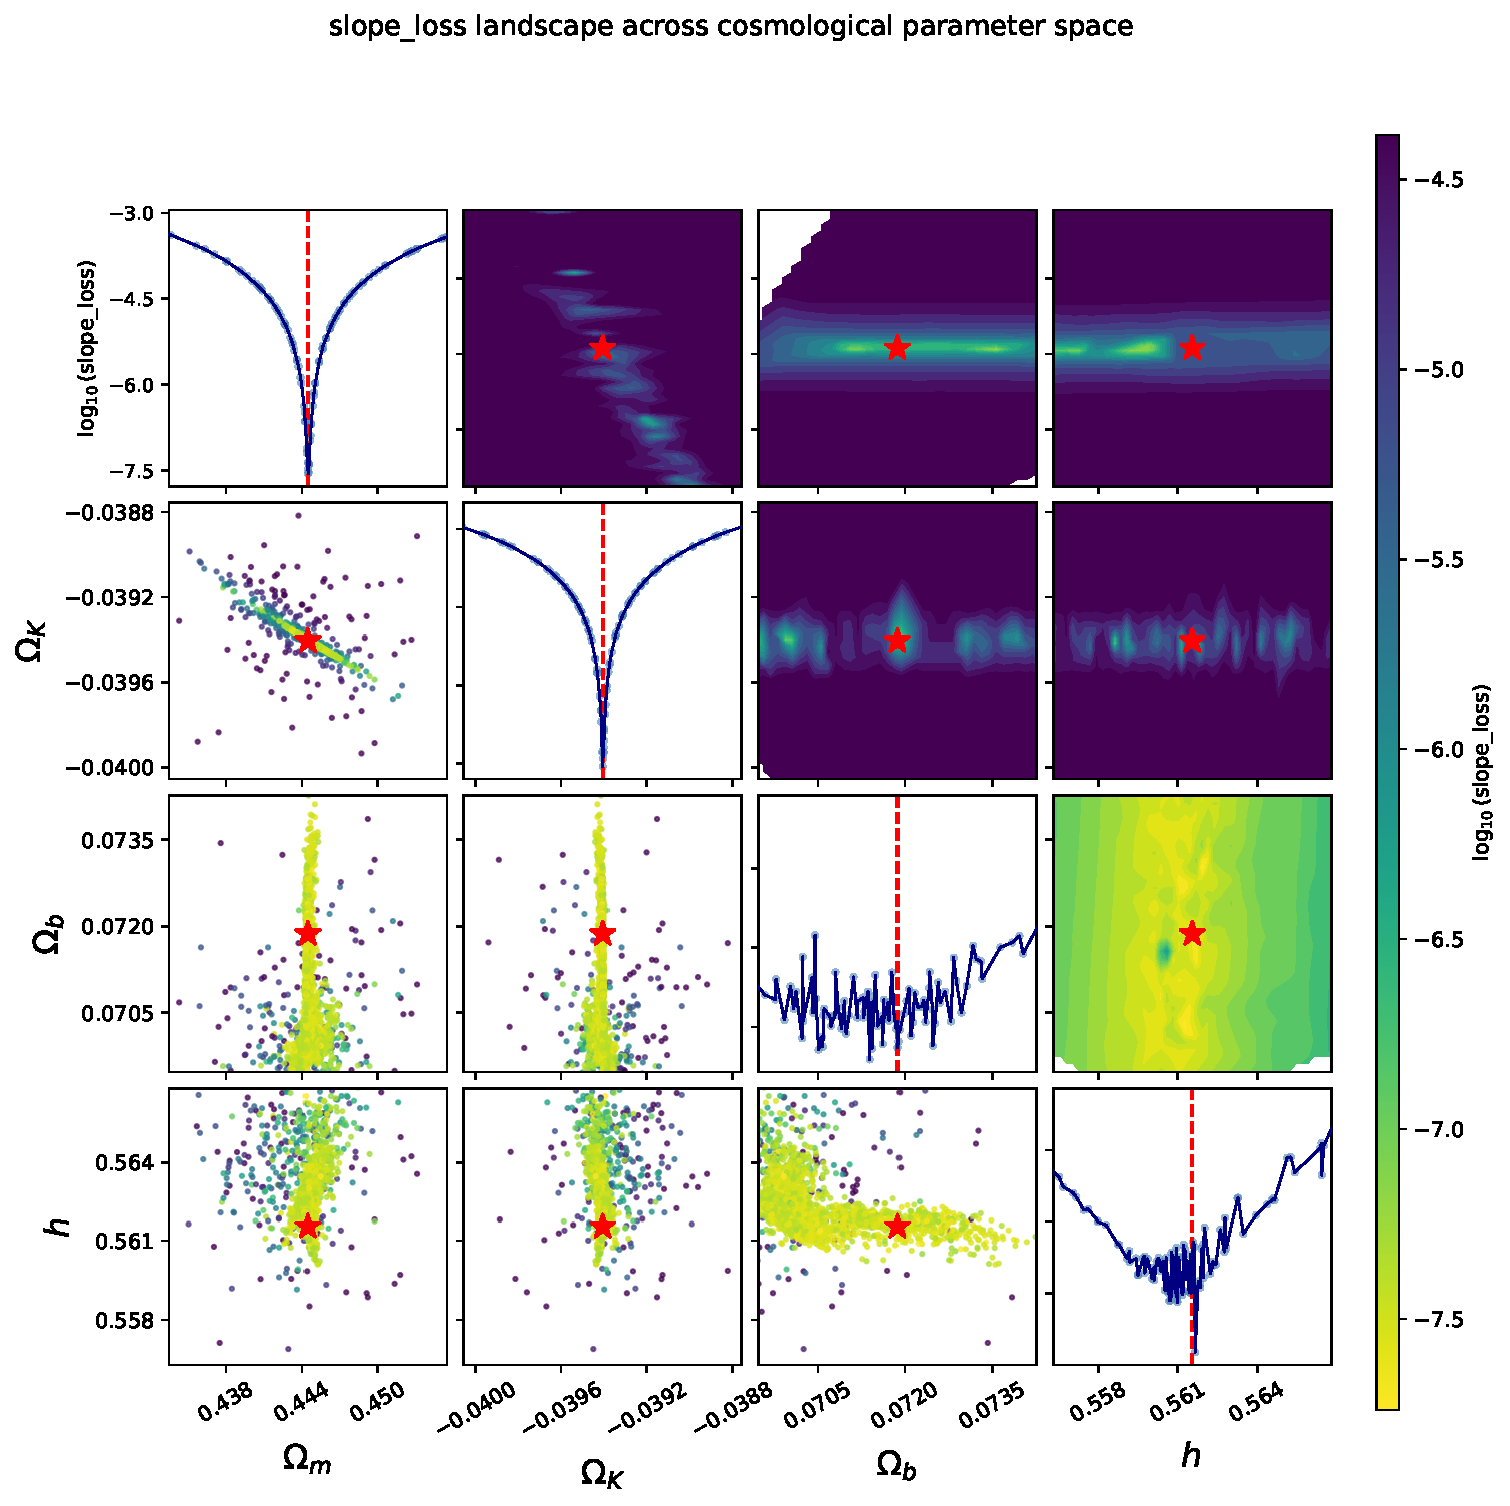
\includegraphics[width=\textwidth]{parts/part1/figures/loss_param_space_Omegab.pdf}
     \caption{The lower triangle contains scatter plots generated by \texttt{Optuna} during the minimization of the integer spacing loss function. The upper triangle displays 2D slices of the loss function where only two parameters are varied, with the others fixed at their best-fit values. The diagonal subplots display the 1D loss functions.}
     \label{fig:loss_param_space}
\end{figure*} 

Finally, we must fix the primordial parameters $A_s, n_s,$ and $\tau$. Because these parameters do not influence the background expansion history, they cannot be constrained by the $k$-spacing requirement. Instead, they govern structure growth and must be fitted directly to observation. We again employ \texttt{Optuna} to find the best-fit $A_s, n_s,$ and $\tau$ by comparing generated spectra to the \texttt{Planck 2018} data. The optimal values yielding the lowest $\Delta\chi^2$ are: $A_s=2.1805\times 10^{-9}$, $n_s=0.9672$, and $\tau=0.0724$. 


\subsection{Coupled Multi-Field Perturbations} 

In a realistic cosmological framework, the evolution involves a minimum of six coupled perturbations: $\Phi, \Psi, \delta_r, \delta_m, v_r, v_m$, supplemented by higher-order Boltzmann moments. To find a single, unified set of linear combination coefficients that simultaneously matches all perturbations across both BCs, the variables must be mathematically concatenated into a single effective field vector: 
\begin{equation}\label{eq:linear_combine_multi_fields}
\begin{aligned}
    \mathbb{X}=\begin{pmatrix}\phi\\\psi\\\delta_r\\\delta_m\\v_r\\v_m \end{pmatrix}, \quad \Phi=\sum_n c_n \mathbb{X}_n=\sum_m c_m \tilde{\mathbb{X}}_m.
\end{aligned}
\end{equation} 
This can also be interpreted as a "stacked" sequential time series, where the effective time coordinate ($\eta$) runs continuously from $0$ to $N\eta_{\text{FCB}}$:
\[ \mathbb{X}(\eta)=\phi(\eta) \oplus \psi(\eta-\eta_{\text{FCB}}) \oplus \delta_r(\eta-2\eta_{\text{FCB}}) \dots\]

Standard linear algebra guarantees that an infinite, complete basis can reconstruct any arbitrary function. In our context, this implies that bases spanning sufficiently high $k$-modes will be able to reliably reconstruct the "stacked" target field, even if hundreds of higher-order Boltzmann terms are strictly included \footnote{In practice, numerically generating bases with a massive number of $k$-modes is computationally prohibitive. Consequently, we limit our current numerical implementation to matching the six primary variables. Nevertheless, the mathematical formalism generalizes natively to include all higher-order terms.}.

\subsection{Phenomenologically Favored Solutions}

To generate the primordial power spectrum (PPS) and CMB power spectrum, phenomenological considerations must be made. Since pure $k\in \mathbb{N}$ modes are conventionally assumed for a closed universe, solutions that most closely resemble isolated integer-$k$ modes are phenomenologically preferred. Analytically, this means we seek a linear combination coefficient matrix $C_{ij}$ that is as sparse as possible, ideally approaching an identity matrix.

With all constraints defined, we search for valid perturbation solutions using \textbf{Canonical Correlation Analysis (CCA)}. CCA normalizes the disparate bases and computes the mutually consistent eigenvectors simultaneously. These global eigen-solutions are then rotated into their sparsest possible representation via an oblique rotation algorithm (\texttt{Promax}), which is specifically designed for non-orthonormal bases. For a rigorous breakdown of the CCA and \texttt{Promax} methodologies, refer to \cref{sec:CCA_sparse}. 

The resulting sparse solutions are shown in \cref{fig:cca_timeseries}. The specific perturbation time series $\delta_r, \delta_m, v_r,$ and $v_m$ generated by the allowed-$k$ basis and the integer-$k$ basis are perfectly aligned, proving that they are valid solutions satisfying both spatial and temporal BCs simultaneously \footnote{Because the metric potentials $\Phi$ and $\Psi$ are strictly determined by $\delta_r, \delta_m, v_r,$ and $v_m$ (via Eq.~6 in \cite{pjz6-47jv}), matching the fluid variables guarantees that the metric variables also match.}. Examining the temporal BC specifically, the density perturbations $\delta_r$ and $\delta_m$ must be symmetric at the Future Big Crunch (FCB). As shown, their temporal derivatives cleanly approach zero at the FCB. Conversely, the velocity perturbations $v_r$ and $v_m$ must be anti-symmetric, and their respective curves correctly cross zero at the FCB.

\begin{figure*}[htbp]
     \centering
     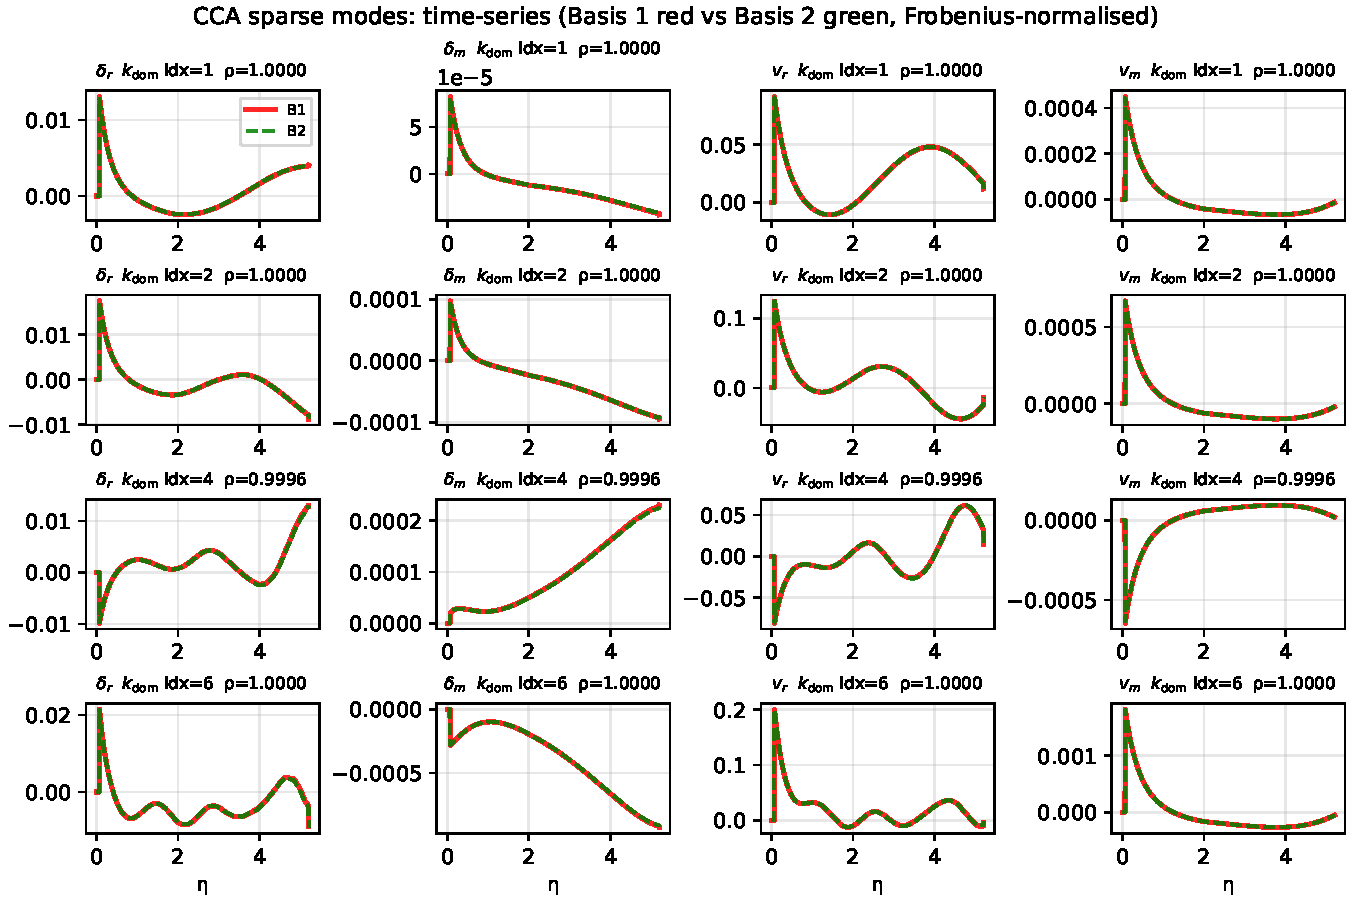
\includegraphics[width=\textwidth]{parts/part1/figures/cca_timeseries.pdf}
     \caption{The first four valid perturbation solutions with the lowest dominant $k$. The time series reconstructed from the allowed-$k$ basis and the integer-$k$ basis overlap exactly, confirming that the solutions successfully satisfy both spatial and temporal boundary conditions.}
     \label{fig:cca_timeseries}
\end{figure*}

% Editor's note: Corrected a broken reference to the figure here (\cref{heatmap_with_delta_k} -> \cref{fig:heatmap_with_delta_k}) based on the label defined in the LaTeX.
\cref{fig:heatmap_with_delta_k} visualizes the coefficient matrix (projected onto the integer-$k$ basis) for the valid sparse solutions. The x-axis represents the available integer-$k$ indices, and each column contains the specific coefficients for a valid composite solution, sorted by its dominant $k$-mode. The lower panel tracks the numerical difference between the temporally allowed $k$-modes and integer-$k$ (defined as allowed-$k$'s nearest integers) \footnote{Because the integer-$k$ sequence is derived by rounding the allowed-$k$ sequence, a sawtooth pattern of residuals naturally emerges. At low $k$, the allowed $k$-spacing is highly non-integer, causing this discrepancy to accumulate rapidly. Once the accumulated difference exceeds $0.5$, the rounding shifts to the next integer, manifesting as a sharp jump in the residual track.}. Where this difference is near zero, the two bases naturally align; the valid solution behaves essentially as a pure mode, and the local coefficient matrix approximates an identity matrix. Conversely, large differences force the CCA to actively mix multiple modes or omit them entirely to maintain consistency. The physical ramifications of this mode mixing and omission on the PPS and CMB are analyzed below.

\begin{figure}[htbp]
     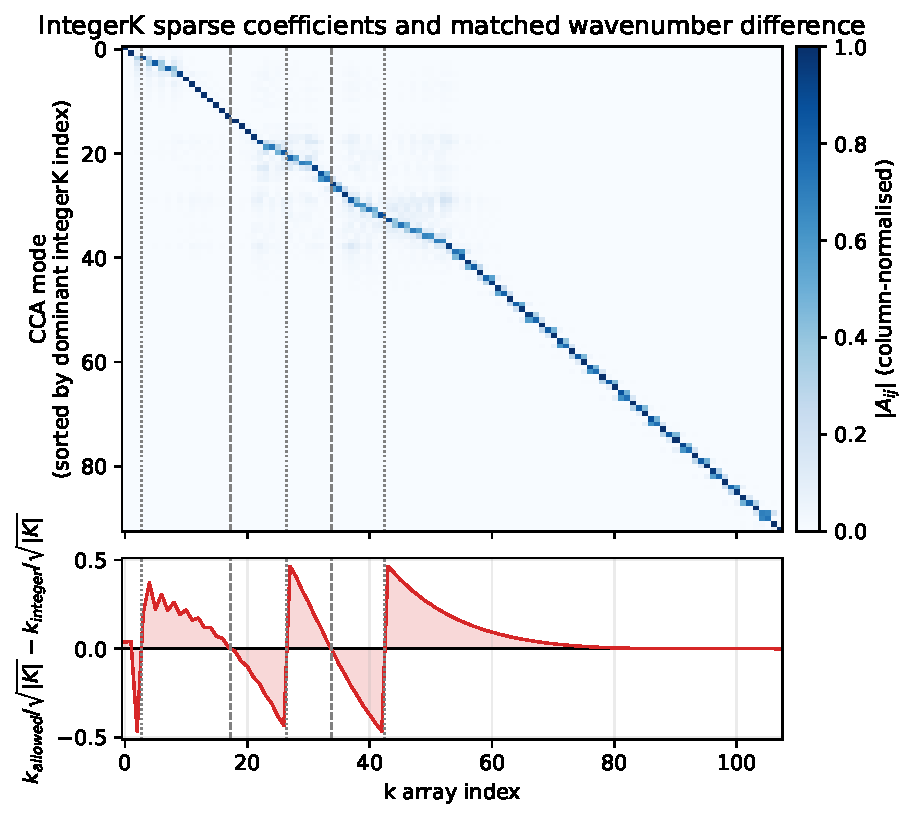
\includegraphics[width=0.8\textwidth]{parts/part1/figures/cca_integerK_heatmap_with_delta_k.pdf}
     \centering
     \caption{Top: Heatmap of the linear combination coefficients for valid sparse solutions. Bottom: The numerical difference between the allowed-$k$ values and the reference integer-$k$ values. Regions of high and low discrepancy are highlighted with dotted and dashed lines, respectively.}
     \label{fig:heatmap_with_delta_k}
\end{figure} 

\section{Generation of Primordial Power Spectra and CMB Spectra}\label{sec:PPS_CMB}

To generate the CMB power spectrum, a fully self-consistent treatment would require extracting the raw perturbation basis directly from a Boltzmann code (e.g., \texttt{CLASS}), executing the CCA to find valid superpositions, and then feeding those exact coupled time-evolutions back into the code to evaluate the true line-of-sight integration internally. However, extensively modifying a standard Boltzmann solver to accommodate this framework is a substantial undertaking that lies beyond the scope of this chapter. (We anticipate that the advancements in large language models may facilitate this complex software engineering task). For the present study, we employ several simplifying assumptions to outline the qualitative effects of this theory on cosmological observables.

In the previous section, we have isolated the sparse valid solutions $\Phi_\lambda$ that satisfy both BCs. Now we use them to construct the PPS and CMB power spectra. The true physical field should be a generalized linear combination of these valid eigenmodes: $\varPhi_{\text{true}}(x) = \sum_\lambda c_\lambda \Phi_\lambda(x)$, where the variance of the coefficients $c_\lambda$ is fundamentally dictated by the PPS.

We hypothesize that the underlying primordial generation mechanism (e.g., inflation) produces an effective spectrum identical to the standard scale-invariant expectation: $P_{std}(k)=A_s(k/k_\star)^{n_s-1}$, where the parameters $A_s$ and $n_s$ are fixed by the early universe physics. Accordingly, the variance of the physical coefficients $c_\lambda$ is assigned as:
\[ \langle |c_\lambda|^2 \rangle =A_s (k_{dom}/k_\star)^{n_s-1}\]
where $k_{dom}$ is the dominant $k$-mode of the specific composite solution $\Phi_\lambda$.

To derive the observable PPS, one must sum the specific fractional contributions across all valid solutions at a given integer $k$:
\begin{equation}
    P_{obs}(k) = \sum_\lambda \langle |c_\lambda|^2 \rangle \times |a_{\lambda k}|^2
\end{equation}
Crucially, $P_{obs}(k)$ naturally reduces to the standard $P_{std}(k)$ in regimes where all valid solutions are pure integer-$k$ modes (i.e., when $a_{\lambda i}=\delta_{\lambda i}$ and $k_{dom}=k$). 

The resulting PPS is presented in \cref{fig:PPS_cca}. We observe a distinct, general power suppression accompanied by severe fluctuations in the low-$k$ region. This is a direct consequence of the omitted and heavily mixed modes necessitated by the boundary mismatches at low $k$ (as mapped in \cref{fig:heatmap_with_delta_k}). Moving to higher frequencies, there is a stable plateau between $k \approx 1.8 \times 10^{-3} \text{ Mpc}^{-1}$ and $3.3\times 10^{-3} \text{ Mpc}^{-1}$, corresponding perfectly to the first identity-matrix region in \cref{fig:heatmap_with_delta_k} where the two bases momentarily synchronize. Finally, at high $k$ ($k > 9\times 10^{-3} \text{ Mpc}^{-1}$), the PPS permanently asymptotes back to the standard scale-invariant model as the asymptotic spacing of the allowed modes converges to integers.
% However, there is lots of wiggling. It is because numerical issue. At high k, the mode completes many oscillations between recombination and the FCB. The phase accumulated is $φ ≈ k·(η_{FCB} − η_{rec})$. A shift of $Δk$ shifts the final phase by $Δφ ≈ Δk·(η_{FCB} − η_{rec})$. Because $Δk$ is small but $(η_{FCB} − η_{rec})$ is large, $Δφ$ can be an arbitrary fraction of $2π$, placing the integerK solution at a completely different phase at the FCB relative to the allowedK solution — hence the shape of perturbations quite different for integerK despite $Δk/k$ being tiny. 

\begin{figure}
     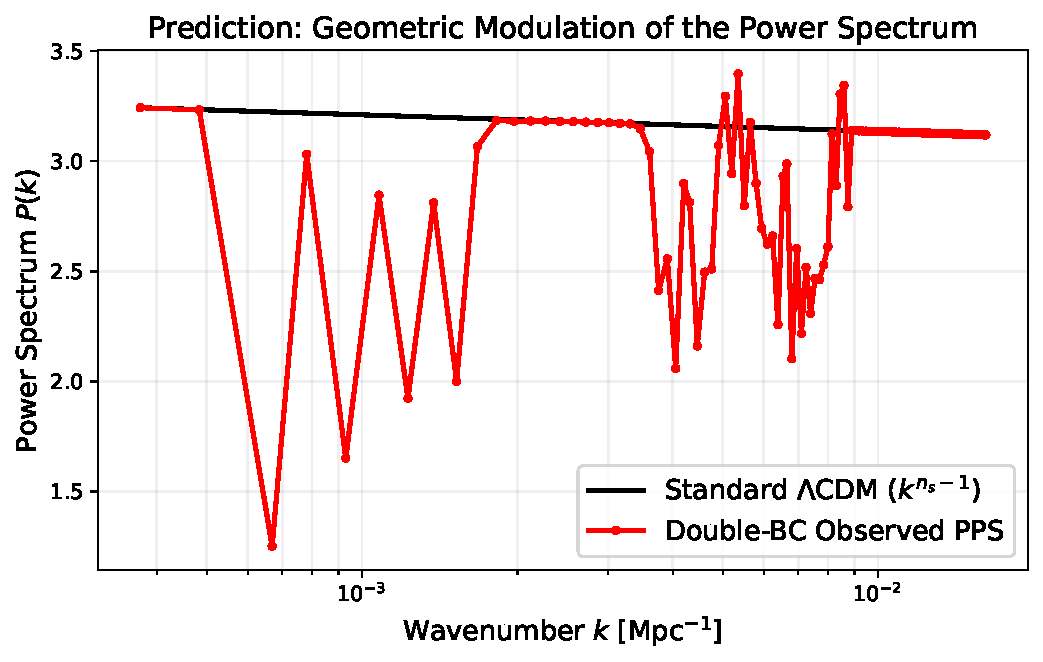
\includegraphics[width=0.75\textwidth]{parts/part1/figures/PPS_power_spectra_cca_2D_dk_penalty_smooth_highK_As_ns_tau_bestfit.pdf}
     \label{fig:PPS_cca}
     \centering
     \caption{The predicted PPS resulting from the valid linear combined solutions. Notably, there is a pronounced suppression and high-variance fluctuation in the low-$k$ regime, which smoothly transitions back to a standard scale-invariant spectrum at high $k$.}
\end{figure} 

Finally, we inject this modified PPS into the Boltzmann solver \texttt{CLASS} to evaluate its impact on the observable CMB temperature power spectrum. The results are plotted in \cref{fig:CMB_cca}. 
% \footnote{$C_\ell^{EE}$ and $C_\ell^{TE}$ are ignored, since the signal are both approach to zero in low $\ell$ mode, making it hard to be distinguished from the standard one}. 
As expected, the suppressions and fluctuations present in the low-$k$ PPS are transferred directly into the low-$\ell$ CMB multipoles. Interestingly, these generic features possess the potential to physically explain longstanding anomalies observed in the \texttt{Planck 2018} dataset \footnote{For instance, the anomalously low quadrupole ($\ell = 2$) relative to the standard $\Lambda\text{CDM}$ theoretical prediction, as well as the higher variance scatter in adjacent low-$\ell$ bins.}. Unfortunately, the inherently large cosmic variance at these scales limits the statistical significance of any such comparison. Because this variance is a fundamental statistical limit arising from having only one observable universe, it cannot be overcome by simply increasing CMB detector resolution. Definitively confirming this model will likely require independent 3D probes of ultra-large-scale structure, such as future galaxy surveys or 21cm intensity mapping arrays, to break this statistical degeneracy.

\begin{figure}
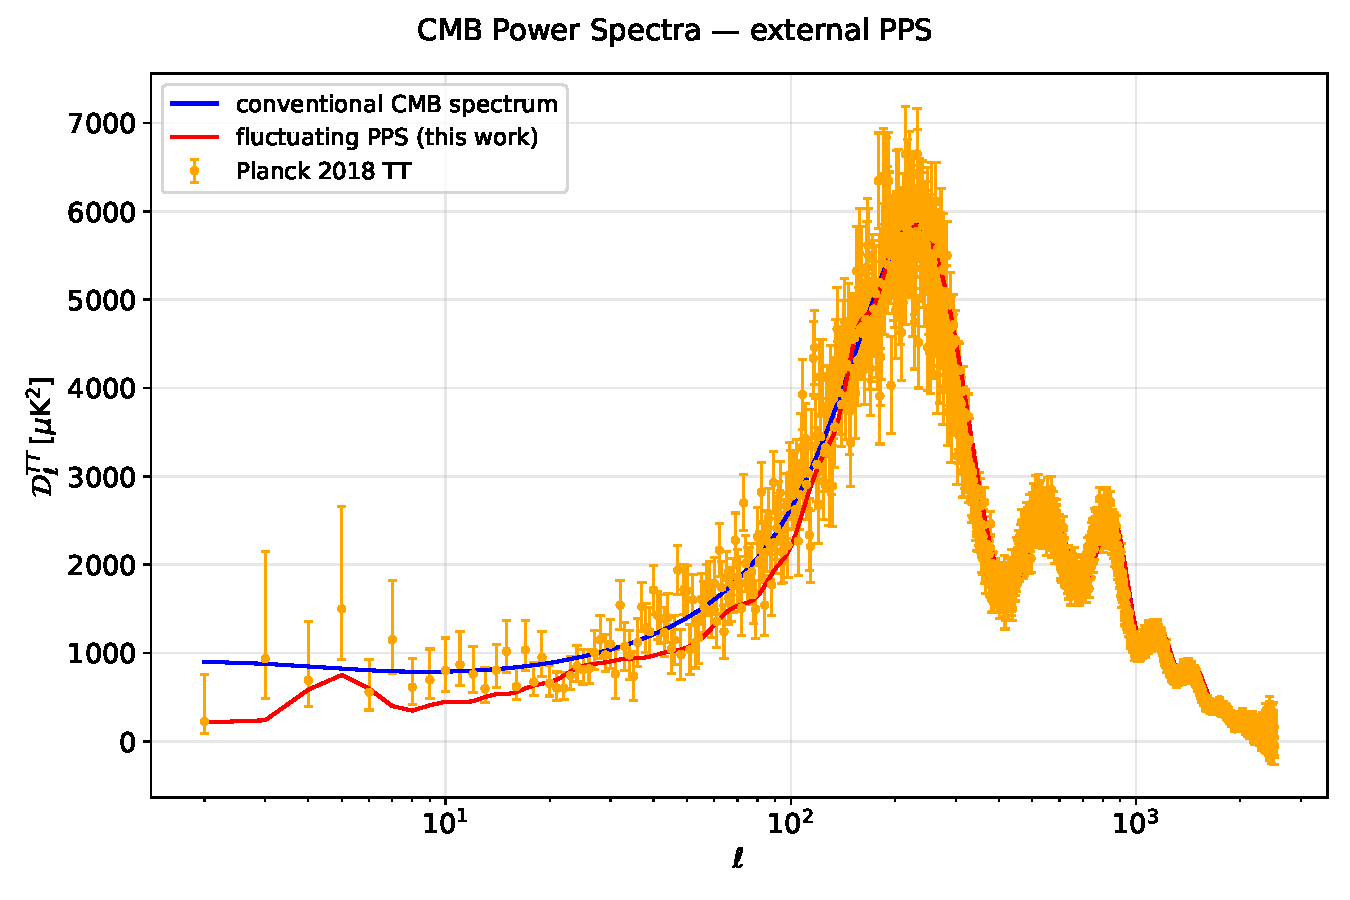
\includegraphics[width=0.9\textwidth]{parts/part1/figures/CMB_TT_externalPPS.pdf}
     \centering
     \caption{The CMB power spectrum generated using our modified PPS. The distinct suppression and fluctuation signatures at low $\ell$ are driven entirely by the constraints imposed by the dual boundary conditions.}
     \label{fig:CMB_cca}
\end{figure} 

Before concluding this analysis, we would like to emphasize again the assumption and simplification utilized in this pipeline. The methodologies for defining "sparse" acceptable solutions and prescribing the generative coefficients $c_\lambda$ rely on numerical and phenomenological assumptions. Furthermore, the modified PPS was externally forced into \texttt{CLASS} to generate the final CMB curves, without directly modifying the Boltzmann code for the theory.  

Due to these simplifications, the exact multipole positions and specific amplitudes of the fluctuations predicted in \cref{fig:CMB_cca} remain approximate. Substantial numerical work is required to elevate this pipeline to a strictly predictive standard. Consequently, this study should be viewed as a pioneering demonstration of the theoretical necessity of these unified solutions, and a qualitative mapping of how imposing dual boundary conditions irrevocably alters the low-$k$ observable universe.


\section{Future Directions}\label{sec:future_work}

This framework offers a novel paradigm for stress-testing fundamental models of the early universe. Alternative theoretical models—such as specific models of cosmic inflation, quantum initial conditions, modified gravity, or loop quantum cosmology—will inherently predict different baseline PPS profiles, coupled perturbation equations, or foundational temporal and spatial boundary constraints. When processed through our dual-BC matching framework, these varying inputs will produce distinct, model-specific valid solution sets and distinct structural mode-mixing matrices. This, in turn, will manifest as highly specific, testable interference features in the observable CMB \footnote{Provided, of course, that the computational simplifications discussed in the previous section are successfully resolved.}.

Beyond the specific spectral fluctuations, one might ask how else this overarching theory could be empirically validated. Since the spectral distortions are strictly localized to the low-$k$ regime, large-scale structures and the CMB remain the primary direct observables. However, the requirement that the allowed $k$-modes approach integer spacing provides a rigid, independent constraint on the background cosmological parameters themselves \cite{pjz6-47jv} \footnote{If the intercept phase of the allowed-$k$ modes can be accurately modeled and included in the loss function, these constraints would become even tighter, particularly for parameters like $\Omega_b$ that subtly govern the phase shifts across recombination.}. If upcoming high-precision surveys independently confirm cosmological parameters that tightly align with the narrow allowed bands predicted by this periodic model, it would represent compelling circumstantial evidence for our model.

Finally, the mathematical methodology developed here for determining valid solutions in systems with competing spatial and temporal boundary conditions has broad applicability across other domains of physics. While temporal boundary conditions appear uniquely exotic in the context of cosmology, they are mathematically ubiquitous in any tightly constrained oscillatory system. For instance, any physical field confined within a finite spatial cavity that is also driven or constrained to oscillate at fixed specific frequencies presents an identical mathematical challenge. Given the coupled PDEs for such a system, our CCA and oblique rotation pipeline provides a generalized toolkit for extracting the non-trivial, physical resonant modes.


\section*{Data Availability Statement}
The source code and data used for generating all figures and results in this study is publicly available in the GitHub repository \cite{code_for_figures_26xx.xxxx} and Zenodo \cite{code_for_figures_26xx}.

\begin{subappendices}

\section{Canonical Correlation Analysis and Sparse Solutions}\label{sec:CCA_sparse}

\subsection{Problem Statement}

A Boltzmann code produces solutions for cosmological perturbation variables \(\Phi,\Psi,\delta_r, \delta_m, v_r, v_m\) (and various higher-order Boltzmann terms) as functions of conformal time $\eta$ and wavenumber $k$. For a given set of $N_k$ wavenumbers, we generate two distinct bases of solutions:

\begin{itemize}
    \item \textbf{Basis 1} (e.g., integer-$k$): defined by matrices $X^p$ of shape $(N_\eta, N_k)$ for each perturbation type $p$,
    \item \textbf{Basis 2} (e.g., allowed-$k$): defined by matrices $\tilde X^p$ of the same shape,
\end{itemize}
where the rows index conformal time and the columns index the independent $k$-modes.

We seek sets of linear combination coefficient vectors such that the composite time evolution constructed using Basis 1 matches the composite time evolution constructed using Basis 2, simultaneously across all required perturbation types. The desired final result is a set of \textit{sparse} coefficient vectors, where each vector is concentrated on one (or very few) $k$-modes, effectively representing the fundamental, physical joint eigenfunctions of the two conflicting bases.


\subsection{Methodology of Canonical Correlation Analysis and Sparsity}
\subsubsection{The Stacked-SVD Approach}

We first rescale the data matrix for each perturbation type in both bases by its respective Frobenius norm, $\|A\|_F = \sqrt{\sum_{ij} A_{ij}^2}$, defining:
\begin{equation}
\bar{X}^p = \frac{X^p}{\|X^p\|_F},\quad \bar{\tilde X}^p = \frac{\tilde X^p}{\|\tilde X^p\|_F}.
\end{equation}
These normalized arrays are then vertically stacked to create a single master state vector:
\begin{equation}
\mathbb{{\bar X}} = \begin{pmatrix}
\bar{X}^{\delta_r} \\
\bar{X}^{\delta_m} \\
\bar{X}^{v_r} \\
\bar{X}^{v_m}
\end{pmatrix}, \quad \mathbb{{\bar {\tilde X}}} = \begin{pmatrix}
\bar{\tilde X}^{\delta_r} \\
\bar{\tilde X}^{\delta_m} \\
\bar{\tilde X}^{v_r} \\
\bar{\tilde X}^{v_m}
\end{pmatrix}.
\end{equation}
Note that the metric potentials $\Phi$ and $\Psi$ are not directly included in the stack, as their dynamics are strictly locked to the fluid variables via the constraint equations. Higher-order Boltzmann moments are also excluded in this specific numerical implementation to control computational overhead (any number of variables can theoretically be added, provided the basis size $N_k$ is correspondingly increased to provide sufficient degrees of freedom). 

This stacking produces unified state matrices of shape $(4N_\eta, N_k)$. While one could technically apply standard SVD to these stacked matrices directly, this formulation obscures the geometric structure of the problem. Stacking is essentially an ad hoc computational trick to collapse a multi-field system into a single matrix, and the Frobenius rescaling represents a specific, non-unique choice for handling the diverse physical dimensions of the variables. For notational simplicity in the following derivations, we will \textbf{drop the bar notation}, but it should be understood that all data matrices are inherently Frobenius-rescaled.

\subsubsection{Formulating Gram Matrices in Momentum Space }

We introduce a set of positive, dimensionless weighting factors $\{w_p\}$ indexed by the perturbation type \footnote{In principle, one could simply set all $w_p=1$. However, because CCA seeks to maximize total covariance, the objective function would otherwise be overwhelmingly dominated by highly oscillatory, high-variance perturbations (e.g., radiation modes). Setting deliberate weights ensures that slower-evolving modes (e.g., $\delta_m$) hold equal footing during the alignment computation.}. We define the $k$-space Gram matrices from the Frobenius-rescaled data as follows:
\begin{equation}
\begin{aligned}
    G_1\equiv G = \sum_p w_p ({X}^p)^\top {X}^p,\\
    G_2\equiv\tilde G = \sum_p w_p (\tilde{X}^p)^\top \tilde{X}^p,\\
    G_{12}\equiv M = \sum_p w_p (X^p)^\top \tilde{X}^p.
\end{aligned}
\end{equation}
Each of these matrices has the shape $(N_k, N_k)$. Because the input data have been normalized, these Gram matrices remain strictly dimensionless regardless of the original physical units of the underlying perturbation fields \footnote{The initial Frobenius rescaling successfully absorbs the per-basis and per-type scale factors, ensuring that $G_{12}$ automatically carries the geometrically correct cross-scaling $(\|X_1^p\|_F \|X_2^p\|_F)^{-1}$ for each term.}.

The matrices $G_\alpha$ (where $\alpha \in \{1,2\}$) strictly encode the inner products between the $k$-modes as measured across all active perturbation types within basis $\alpha$, acting as normalization metric tensors (analogous to the normalization procedure discussed in \cref{sec:linear_combine_solution}). Meanwhile, $G_{12}$ encodes the cross-correlation maps between the two distinct bases, fulfilling the role of the projection matrix $M$ introduced in \cref{sec:linear_combine_solution}.

\subsubsection{Two-Vector Canonical Correlation Analysis}

CCA seeks two linear combination coefficient vectors—$\boldsymbol{c} \in \mathbb{R}^{N_k}$ for Basis 1 and $\boldsymbol{\tilde c} \in \mathbb{R}^{N_k}$ for Basis 2—that maximize the normalized correlation between their resultant time evolutions:
\begin{equation}\label{eq:cca_correlation}
\rho(\boldsymbol{c}, \boldsymbol{\tilde c}) = \frac{\boldsymbol{c}^\top M \boldsymbol{\tilde c}}{\sqrt{\boldsymbol{c}^\top G \boldsymbol{c} \cdot \boldsymbol{\tilde c}^\top \tilde G \boldsymbol{\tilde c}}}.
\end{equation}
The physical intuition here is clear: $\sqrt{G}\boldsymbol{c}$ represents the amplitude of the combined solution reconstructed within the properly normalized Basis 1 metric, and $\sqrt{\tilde G}\boldsymbol{\tilde c}$ represents the same for Basis 2. \cref{eq:cca_correlation} is simply the inner product of these two reconstructed solutions normalized by their respective lengths, which achieves a maximum of $1$ only when the solutions are functionally identical.

This mathematical operation formally mirrors the geometric projection method described conceptually in \cref{sec:linear_combine_solution}, but it powerfully automates the normalization, isolates the translation-invariant solutions, and transforms the eigenvectors back into the original, non-orthogonal basis space in a single integrated step. It is straightforward to prove that $\sqrt{G}$ and $\sqrt{\tilde G}$ act precisely as transformation matrices that map the raw bases into an orthonormal frame. Taking Basis 1 as an example: 
\begin{equation}
\begin{aligned}
    T_{ij}\varphi_i &=\phi_j  \implies  \varphi_i=T_{ij}^{-1}\phi_j\\
    \big< \varphi_i| \varphi_j\big>&=\delta_{ij}  \implies  \big< \phi_k|(T^{-1})^\top_{ki} T_{jl}^{-1}\phi_l\big>=\delta_{ij}\\
    |\phi_m\big>&\big< \phi_k|(T^{-1})^\top_{ki} T_{il}^{-1}|\phi_l\big>\big< \phi_n|=|\phi_m\big>\big< \phi_n|\\
    G_{mk}(T^{-1})^\top_{ki} &T_{il}^{-1}G_{ln}=G_{mn} \implies(T^{-1})^\top_{ki} T_{il}^{-1}\\
    =G_{km}^{-1} &G_{mn}G_{nl}^{-1}=G_{kl}^{-1}  \implies  G_{kl}=T^\top_{ki} T_{il}.
\end{aligned}
\end{equation}

Returning to the maximization of \cref{eq:cca_correlation}, the problem is efficiently solved via Singular Value Decomposition (SVD):
\begin{equation}
G^{-1/2} M \tilde G^{-1/2} = U \Sigma V^\top,
\end{equation}
where $\Sigma = \operatorname{diag}(\sigma_1, \sigma_2, \dots)$ such that $\sigma_1 \ge \sigma_2 \ge \dots \ge 0$. The resulting canonical correlations are $\rho_i = \sigma_i$, and their corresponding coefficient vectors are:
\begin{equation}
\boldsymbol{c}_i = G^{-1/2} \boldsymbol{u}_i,\quad \boldsymbol{\tilde c}_i = \tilde G^{-1/2} \boldsymbol{v}_i,
\end{equation}
where $\boldsymbol{u}_i$ and $\boldsymbol{v}_i$ are the $i$-th columns of $U$ and $V$, respectively. Because $U$ and $V$ are evaluated in the normalized frame, we multiply them by the transformation matrices $G^{-1/2}$ and $\tilde G^{-1/2}$ to pull the coefficients back into the physical frame of the original bases ($\boldsymbol{c}_i$ and $\boldsymbol{\tilde c}_i$).

Equivalently, the left canonical vectors $\boldsymbol{c}_i$ can be extracted directly from the generalized eigenvalue problem:
\begin{equation}
G^{-1/2} M \tilde G^{-1} M^\top G^{-1/2} \boldsymbol{u} = \lambda \boldsymbol{u},
\end{equation}
with eigenvalues $\lambda_i = \sigma_i^2 = \rho_i^2$. Modes with $\rho_i \approx 1$ represent physically valid joint eigenfunctions, while modes with $\rho_i \ll 1$ indicate temporal trajectories that are fundamentally incompatible between the two bases.

\subsubsection{Constructing Sparse Bases via Oblique Rotations}

The raw CCA coefficient vectors $\boldsymbol{c}_i$ and $\boldsymbol{\tilde c}_i$ are rarely sparse; they emerge as dense, global linear combinations of many $k$-modes because the solver optimizes purely for correlation with no regard for localization. To recover a physically meaningful basis, we seek an invertible rotation matrix $R \in \mathbb{R}^{m \times m}$ such that the rotated coefficient vectors:
\begin{equation}
\begin{aligned}
    &{\boldsymbol{c}}^R_j = \sum_{i=1}^m R_{ji} \boldsymbol{c}_i, \quad \text{i.e.} \\ {C}^R = C R^\top, &\quad C = [\boldsymbol{c}_1 \mid \cdots \mid \boldsymbol{c}_m] \in \mathbb{R}^{N_k \times m},
\end{aligned}
\end{equation}
become optimally sparse (i.e., tightly concentrated on a single $k$-mode or a small cluster of modes). Notably, we do not require the final rotated vectors ${\boldsymbol{c}}^R_j$ to be orthogonal—only sparse.

A common algorithm for this task is \texttt{Varimax} rotation, which rigidly rotates the sub-space frame to maximize the sum of the variances of the squared loadings. However, \texttt{Varimax} strictly enforces orthogonality, preserving the angles between all vectors during the rotation. Because our physical CCA vectors $\boldsymbol{c}^R_i$ are not fundamentally orthonormal in $k$-space, applying rigid \texttt{Varimax} produces severe alignment errors.

To overcome this, we utilize Oblque rotation method \texttt{Promax}, which generalizes \texttt{Varimax} by actively relaxing the orthogonality constraint. It searches for an invertible matrix $R$ (which need not be orthogonal) that refines the \texttt{Varimax} approximation into a form displaying "simple structure" (maximal sparsity). The additional degrees of freedom allowed by non-orthogonal deformation grant \texttt{Promax} the flexibility needed to find a significantly sparser, and therefore more physical, solution than any strictly orthogonal rotation algorithm. 

% \begin{table}[t]
% \centering
% \begin{minipage}{0.8\textwidth}
% \noindent \hrule \vspace{1em}
% \noindent \textbf{CCA-based sparse joint eigenfunction method}  \\ \vspace{0.5em}
% \noindent \hrule \vspace{1em}
% \noindent \textbf{Input:} $X^p, \tilde X^p \in \mathbb{R}^{N_\eta \times N_k}$ for each perturbation type $p$; weights $\{w_p\}$; correlation threshold $\rho_{\min}=0.99$ \\[0.5em]
% \noindent\begin{tabular*}{\textwidth}{@{}r@{\hspace{0.5em}}l@{\extracolsep{\fill}}r@{}}
% 1: & \textbf{Frobenius rescaling}  \\
% 2: & \quad $\bar{X}^p \leftarrow X^p/\|X^p\|_F$ for all $p$, similarly for $\bar{\tilde X}^p$ & \\[0.5em]
% 3: & \textbf{Compute Gram matrices}   \\
% 4: & \quad $G \leftarrow \sum_p w_p ({X}^p)^\top {X}^p$ \\
% 5: & \quad $\tilde G \leftarrow \sum_p w_p (\tilde{X}^p)^\top \tilde{X}^p$ & \\
% 6: & \quad $M \leftarrow \sum_p w_p ({X}^p)^\top \tilde{X}^p$ & \\[0.5em]
% 7: & \textbf{Solve CCA}  \\
% 8: & \quad $U \Sigma V^\top \leftarrow \text{SVD}(G^{-1/2} M \tilde G^{-1/2})$ & \\
% 9: & \quad Keep $m$ components with $\sigma_i > \rho_{\min}$ & \\
% 10: & \quad $\boldsymbol{c}_i \leftarrow G^{-1/2} \boldsymbol{u}_i$ for $i=1,\dots,m$ & \\ &$\triangleright$ Basis 1 $k$-space coefficients \\
% 11: & \quad $\boldsymbol{\tilde c}_i \leftarrow \tilde G^{-1/2} \boldsymbol{v}_i$ for $i=1,\dots,m$ & \\ &$\triangleright$ Basis 2 $k$-space coefficients \\[0.5em]
% 12: & \textbf{Oblique rotation for sparsity} \\
% 13: & \quad $C \leftarrow [\boldsymbol{c}_1 \mid \cdots \mid \boldsymbol{c}_m]$  \\
% 14: & \quad ${C}^R \leftarrow \text{Promax}(C)$ \\
% \end{tabular*} \\[0.5em]
% \noindent \textbf{Output:} $C^R \in \mathbb{R}^{N_k \times m}$ \\
% \hspace*{1.5em} Each column: sparse coefficient vector for a valid joint eigenfunction \\
% % \hspace*{1.5em} For modes with $\rho \approx 1$: $\boldsymbol{c}_i \approx \boldsymbol{\tilde c}_i$ (same coefficients in both bases) \\[0.3em]
% \hspace*{1.5em}
% \noindent \hrule
% \end{minipage}
% \end{table}

\end{subappendices}

\printbibliography[heading=subbibintoc, title={References for Chapter \thechapter}]
\chapter{Conclusion and Future work}\label{chapter:conclusion_matter_evol}

\chapterabstract{In this chapter, I first conclude this part of the thesis, and outline several compelling questions and future applications arising from this work. Specifically, we discuss (1) whether the imaginary time period should be considered as an other additional boundary constraint, (2) whether the constraints derived in our model can be leveraged to theoretically predict cosmological parameters via thermodynamics, and (3) whether this framework could be used to indirectly detect non-trivial spatial topologies of the universe. Finally, we discuss the issue of negative matter density--as an odd function of scale factor, it switch signs when transitioning into the anti-universe. To resolve this paradox, we abandon the classical fluid approximation—which inevitably breaks down near cosmological singularities—and instead solve the fundamental quantum field equations near the Big Bang and the end of the universe. We validated this framework in scalar fields, and extending it to fermions naturally leads to the second part of the thesis.} 


\section{Conclusion}
In this Part of the thesis, we investigated the evolution of cosmological perturbations within a globally periodic universe. We derived analytic solutions to the first-order perturbation equations and imposed temporal boundary conditions (BCs) at the future conformal boundary (FCB). These conditions require the perturbations to be strictly symmetric or antisymmetric at the FCB, yielding a discrete spectrum of temporally allowed wave vectors. In \cref{chapter:theory}, we demonstrated that this temporally discrete spectrum is generically incompatible with the integer wave vectors demanded by the spatial compactness of a closed universe. However, because both sets of discrete \(k\) values exhibit equal, uniform spacing in the high-\(k\) regime, they can be formally reconciled by requiring the asymptotic spacing of the temporal modes to be an integer. Because this mode spacing is inversely proportional to the conformal age of the universe—a quantity highly dependent on spatial curvature—this matching condition rigidly constrains $\Omega_K$ to a specific set of discrete values. 

To facilitate a direct comparison with observational data, in \cref{chapter:Observation}, we evaluated the temporally discrete \(k\) spectrum by numerically solving the coupled perturbation equations, explicitly incorporating both matter and radiation anisotropies. The integer-spacing requirement was then utilized as a physical constraint to filter the \texttt{Planck 2018 MCMC} chains. This analysis yielded tight, predictive constraints not only on spatial curvature, but also on the broader set of background cosmological parameters that dictate the age of the universe. 

Finally, in \cref{chapter:low-k}, we extended this framework to the low-\(k\) regime, where the equal-spacing approximation fundamentally breaks down. We established that general solutions capable of satisfying both spatial and temporal BCs simultaneously must be constructed as linear combinations of the two respective bases. Geometrically, these physically valid solutions lie exactly at the intersection of the two basis subspaces, ensuring they remain invariant when projected back and forth between the spatial and temporal coordinate frames. Because the functional discrepancy between the two bases is highly significant at low frequencies, enforcing these dual constraints actively induces mode mixing and mode omissions. We subsequently generated the corresponding primordial and CMB power spectra from these unified solutions, revealing that the low-\(k\) modes exhibit a distinct power suppression accompanied by oscillatory features. Intriguingly, these theoretically derived signatures are phenomenologically consistent with long-standing anomalies observed in the CMB power spectrum.

\section{Future work}

In this section, we discuss three questions and future applications arising from this work. 

\subsection{Imaginary time period as an additional constraint}
Because the scale factor is periodic in both real and imaginary conformal time, one might ask whether the imaginary period imposes an additional boundary constraint on this model. The answer is no; only the real period dictates the physical boundary conditions for the perturbations. 

Consider a mode evolving as $\Phi\propto e^{i\omega t}$: it oscillates cleanly in real time but diverges exponentially in imaginary time. In standard calculations of gravitational entropy, integrating over the imaginary time period is mathematically valid because one first performs a Wick rotation, transforming the path integral $e^{iS}$ into an exponentially suppressed, well-behaved integral $e^{-S_E}$. However, when analyzing the dynamical evolution of physical perturbations in real spacetime (Lorentzian signature), only the real conformal time period imposes physical boundary constraints.

\subsection{Theoretical prediction of cosmological parameters}
Another compelling question is whether we can theoretically predict the values of other cosmological parameters using thermodynamic principles, bounded by the strict matching constraints derived in our model. This question is particularly interesting because Boyle and Turok \cite{2024PhLB..84938442B} demonstrated that universes with a smaller cosmological constant $\lambda$ and spatial curvature $\kappa$ possess higher gravitational entropy, making them statistically more probable. However, their framework could not predict the exact physical values of these parameters. 

To proceed, one could hypothetically calculate the thermodynamic expectation values of these parameters (where $S$ is the gravitational entropy). Taking the cosmological constant $\lambda$ as an example, the expectation value would be: 
\[ \big<\lambda\big>=\frac{\sum_{\lambda,r,m,\kappa}\lambda e^{S[\lambda,r,m,\kappa]}}{Z},\qquad Z=\sum_{\lambda,r,m,\kappa} e^{S[\lambda,r,m,\kappa]} \]

However, a critical problem arises: the partition function sum over the continuous parameter space diverges (e.g., as $\kappa\rightarrow 0$, $S\rightarrow\infty$). At first glance, our framework suggests a resolution, as it restricts the permissible cosmological parameters to a strictly discrete set. While this discretization might mathematically regularize the sum, the presence of an infinite sequence of discrete values approaching zero means the sum could still diverge under these constraints.

Alternatively, expectation values could be rigorously defined by differentiating the partition function, analogous to standard statistical mechanics: 
\begin{equation}
\begin{aligned}
    \big<E\big>&=\frac{\sum_E Ee^{-\beta E}}{Z},\qquad Z=\sum_E e^{-\beta E}\\
\rightarrow \big<E\big>&=-\partial_{\beta}\log Z
\end{aligned}
\end{equation}
Even if the raw partition function diverges, its logarithmic derivatives (and thus the physical expectation values) might remain finite and theoretically predictive.

\subsection{Detecting the topology of the universe}

While the most recent cosmological data are highly consistent with the simplest model of a zero-curvature, infinite universe, they remain equally compatible with compact topologies of homogeneous and isotropic geometries with small curvature. Examples include the spherical Poincaré dodecahedral space, the flat hypertorus, or the hyperbolic Picard horn.

There is no fundamental reason forcing space to possess a trivial topology. General relativity is a purely local theory; the Einstein field equations are local partial differential equations relating the metric and its derivatives to the matter-energy content at a specific point. Consequently, a single local metric solution to the Einstein equations can map to multiple—if not infinitely many—globally compatible topologies. For example, a compact hypertorus ($T^3$) and the standard infinite Euclidean space ($E^3$) are locally identical, and relativistic cosmological models describe them using the exact same FLRW equations. The only distinction lies in the global boundary conditions imposed on the spatial coordinates.

Is it possible to detect the global topology of the universe observationally? The search for such compact topologies, such as the hypertorus, is often termed \textit{cosmic crystallography}. Because the universe would be compact, an observer looking far enough would theoretically see repeating patterns or multiple images of the same structures. Observational efforts have attempted to identify such repeating patterns in large-scale structure distributions or within the cosmic microwave background (CMB). However, no conclusive evidence has been found. This null result implies either that the universe lacks a non-trivial global topology, or simply that the fundamental domain is significantly larger than our currently observable horizon. To learn more about the topology of the universe and how to observe it, one can refer to Jeffrey Weeks' book \textit{The Shape of Space} \cite{weeks2020shape}, which provides an excellent introduction to the topic.

Because it is difficult to observe the global topology directly if the fundamental domain is excessively large, one might ask whether it leaves an indirect signature that we can measure. Our framework offers a potential observational pathway. Different compact topologies impose varying spatial boundary conditions; our findings explicitly demonstrate that these conditions strictly quantize the allowed wave vectors. Consequently, the consistency requirement between the spatial and temporal boundary conditions imposes direct constraints on permissible universe topologies. For instance, if the universe is a hypertorus composed of periodic spatial 3D boxes, the physical dimensions of these boxes would rigidly dictate the minimum value and the exact spacing of the discrete wave vectors. Thus, the boundary matching evaluated in this work could serve as a novel method for indirectly probing the global shape of the universe.


\section{Matter field evolution near the Big Bang and the end of the universe}\label{sec:matter_evol} 

At the end of this part, we discuss the issue of negative matter density, which arise since the matter density is an odd function of scale factor $\Omega_m\paroto 1/a^3$, which switch signs when transitioning into the anti-universe. To resolve this problem, we states that near the transition point, i.e. the Bang and the end of the universe, the classical fluid approximation breaks down and the fundamental quantum field needs to be considered. And since the energy density is defined as absolute value of the field, it remains strictly positive. We demonstrate that scalar field solutions to the Klein-Gordon equation are natively symmetric at the Big Bang, whereas only massless scalar fields preserve this symmetry near the future conformal boundary. Finally, we discuss the extension of this framework to fermions, establishing the theoretical foundation for the investigations presented in Part II of this thesis.

\subsection{Negative matter density} 

Throughout this thesis, we evaluate solutions to the Friedmann equation within a periodic universe. However, a hidden theoretical problem arises regarding the matter density: 
\[ 3\frac{\dot a^2}{a^4}=\lambda +\frac{3\kappa}{a^2}+\frac{m}{a^3}+\frac{r}{a^4}, \]
where the terms proportional to $\lambda,\kappa,m,r$ correspond to the cosmological constant, spatial curvature, matter density, and radiation energy density, respectively. Note that the matter density term is the only strictly odd function of the scale factor $a$. This is not a problem when considering only our forward-evolving universe, where the scale factor $a$ remains strictly positive. However, when global periodic solutions are considered, the scale factor smoothly switches signs in the anti-universe (i.e., on the far side of the Big Bang and the Future Conformal Boundary). Naively, this causes the matter density to become negative. Because a strictly negative energy density is physically pathological, and because switching only the matter sign would cause an asymmetry in the global energy densities between the universe and the anti-universe, the symmetric evolution of $a(\eta)$ would be explicitly broken (see Sec.~V in \cite{2022PhRvD.105h3514L}). To resolve this problem computationally, we previously assumed that the matter density must always remain positive, scaling as $\rho_m\propto 1/|a|^3$. The primary goal of this chapter is to provide a rigorous theoretical justification for this absolute value assumption.

One natural hypothesis is that the relation $\rho_m\propto 1/a^3$ is strictly a classical approximation. This approximation is valid only when $H\ll \mu$ (i.e., far away from the initial singularity, when the ambient temperature is much lower than the fundamental particle mass $\mu$), where the matter smoothly behaves as a pressureless perfect fluid. However, when $H\gg \mu$ (i.e., infinitesimally close to the Big Bang), this fluid limit fails, and we must evaluate the evolution of the underlying quantum fields directly.

Specifically, in the regime where $1/H \sim t \gg 1/\mu$, sufficient time elapses for the high-frequency modes of the quantum field to complete numerous oscillations. These rapid oscillations average out, effectively validating the perfect fluid approximation where $\langle \sin(\mu t + kx) \rangle_{\text{oscillations}} \approx \text{fluid}$. In this limit, massive matter reliably behaves as a classical perfect fluid. On the other hand, in the opposite limit close to the Big Bang, where $1/H \sim t \ll 1/\mu$, the field did not have enough time to oscillate, so quantum effects become significant. 

Similarly, at the end of the universe (approaching the future de Sitter boundary, or FCB), the expansion rate $H$ begins to overwhelm the particle mass scale \footnote{Since particles become effectively massless at late times in de Sitter space, which we will discuss in the next section.}. When the exponential expansion of the de Sitter spacetime outpaces the quantum oscillations ($1/H \sim t \ll 1/\mu$), the field ceases to oscillate efficiently. Once again, the field dynamics cannot be time-averaged, causing the classical perfect fluid approximation to break down.

We propose the following theoretical mechanism: if one evaluates the exact quantum field equations near the Big Bang and the FCB, the fundamental energy density of the fields remains strictly positive. For a canonical scalar field, the energy density evaluates to $\rho \propto \frac{1}{2}(\mu^2 + k^2)\phi^2 > 0$. Therefore, when the classical fluid approximation is recovered at intermediate times (far from the singularities), it naturally enforces the effective scaling $\rho_m\propto 1/|a|^3$.

\subsection{Toy model: The scalar field}

To rigorously test this hypothesis, we first analyze the simplest available model: a free scalar field governed by the Klein-Gordon equation. 

The equation of motion for a scalar field in an expanding universe is $\ddot{\phi} + 3H\dot{\phi} + (k^2/a^2 + \mu^2)\phi = 0$, where the dots denote derivatives with respect to physical time $t$. Transforming this equation into conformal time ($\eta$) yields: 
\[ \ddot{\phi} + 3\frac{\dot{a}}{a}\dot{\phi} + (k^2 + \mu^2a^2)\phi = 0, \quad \text{(where dots now denote } d/d\eta \text{)}. \]

To investigate its geometric evolution near the Big Bang, we apply the radiation-dominated limit, $a \propto \eta$. The analytic solutions can be expressed in terms of the confluent hypergeometric function $U$ and the generalized Laguerre polynomial $L$:

\begin{equation}\label{eq:scalarfield_sol_BB}
    \phi_1(\eta )= \frac{ e^{\frac{1}{2} i \mu\eta ^2 } U\left(-\frac{i k^2}{4 \mu},0,-i \mu \eta ^2\right)}{\eta ^2},\qquad
    \phi_2(\eta)=\frac{ e^{\frac{1}{2} i \mu\eta ^2 } L\left({\frac{i k^2}{4 \mu}},-1,-i \mu \eta ^2\right)}{\eta ^2}.
\end{equation}

\cref{fig:scalarField_sol_BB} plots the absolute value of these two independent solutions ($|\phi_1|$ and $|\phi_2|$) in blue and orange, respectively, with $k=\mu=1$. The second solution, $|\phi_2|$, is the physically valid mode because it remains finite exactly at the Big Bang singularity. Crucially, this physical solution is perfectly symmetric before and after the Bang, robustly confirming the global periodic universe paradigm and inherently preserving a positive-definite energy density.

\begin{figure}
     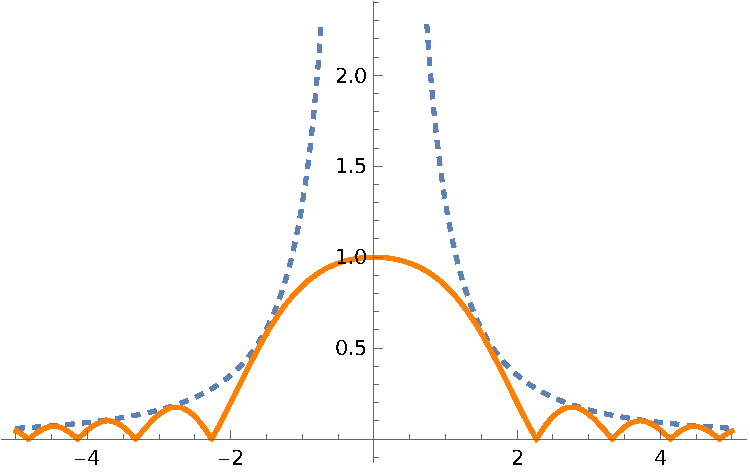
\includegraphics[width=0.5\textwidth]{figures/scalarField_sol_BB.pdf}
     \centering
     \caption{Absolute value of the scalar field solutions near the Big Bang ($\eta=0$). We plot $|\phi|$ because physical energy density is governed by the field amplitude squared.}
     \label{fig:scalarField_sol_BB}
\end{figure}

Next, we evaluate the field evolution near the future conformal boundary (FCB). Modeling the asymptotic de Sitter approach as $a \propto 1/\sqrt{\lambda}(\eta_\infty-\eta)$, the analytic solutions take the form of Bessel functions ($J$ and $Y$): 

\begin{equation}\label{eq:scalarfield_sol_FCB}
    \phi_1(\eta )= \frac{ J_{\sqrt{\frac{\lambda -\mu^2}{\lambda }}}(k \eta -k \eta_{\infty})}{\eta_{\infty}-\eta },\qquad 
\phi_2(\eta)=\frac{ Y_{\sqrt{\frac{\lambda -\mu^2}{\lambda }}}(k \eta -k \eta_{\infty})}{\eta_{\infty}-\eta }.
\end{equation}

\cref{fig:scalarField_m=1_sol_FCB} plots the absolute amplitudes of these solutions (with parameters set to $k=1, \mu=1, \lambda=1,$ and $\eta_\infty=0$). In the presence of a non-zero mass, both independent solutions diverge to infinity at the FCB, rendering them physically pathological.

\begin{figure}
     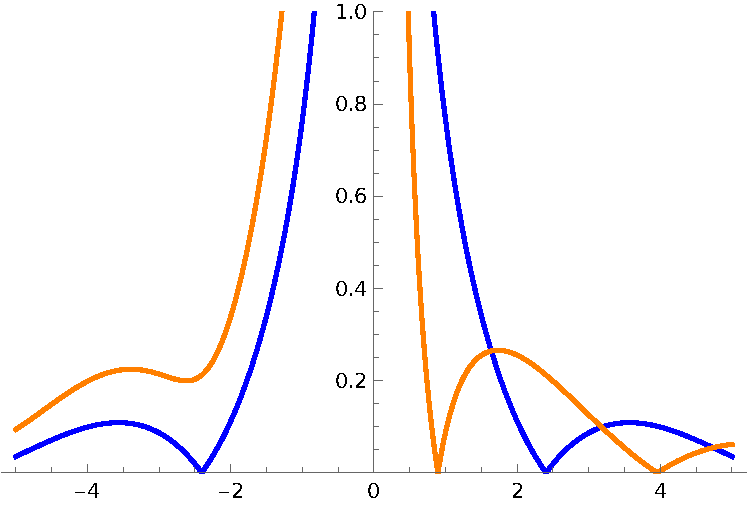
\includegraphics[width=0.5\textwidth]{figures/scalarField_m=1_sol_FCB.pdf}
     \centering
     \caption{Absolute value of the massive scalar field solutions ($|\phi|$) approaching the future conformal boundary ($\eta_\infty=0$). Both solutions are physically divergent.}
     \label{fig:scalarField_m=1_sol_FCB}
\end{figure}

However, if we take the strict massless limit ($\mu\to 0$), the geometric pathology resolves. One of the solutions becomes finite and perfectly symmetric across the boundary:
\begin{figure}
     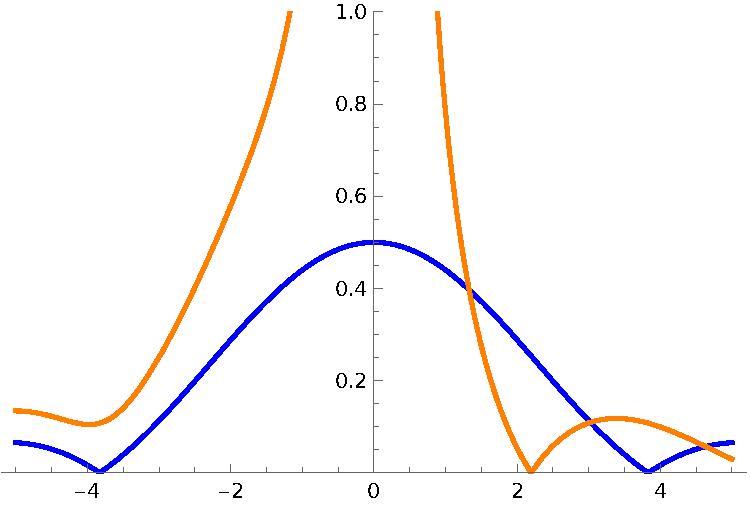
\includegraphics[width=0.5\textwidth]{figures/scalarField_massless_sol_FCB.pdf}
     \centering
     \caption{Absolute value of the nearly massless scalar field solution ($\mu=0.001$) near the end of the universe ($\eta_\infty=0$). The solution is finite and globally symmetric.}
     \label{fig:scalarField_massless_sol_FCB}
\end{figure}

This analysis reveals a profound theoretical constraint: if we couple a massive field ($\mu \neq 0$) to gravity in the standard manner, its quantum mode functions encounter an essential singularity at the future de Sitter boundary. Physically, this occurs because the field attempts to oscillate an infinite number of times (with frequency $\propto \mu$) as coordinate time stretches to infinity near the boundary. Consequently, a stable, well-behaved future boundary condition (such as an analytic Neumann or Dirichlet condition) cannot be imposed. 

However, if physical fields couple to gravity in a non-standard (e.g., strictly Weyl-invariant) fashion—such that their effective mass systematically vanishes as the universe approaches the FCB—well-defined future boundary conditions become theoretically permissible. Several physical mechanisms could drive this effectively massless limit. One possibility is universal particle decay (e.g., proton decay), wherein all massive states eventually decay into massless, strictly Weyl-invariant radiation prior to the FCB. Another highly compelling possibility relates to the ultimate fate of cosmic expansion (the "Big Rip" scenario): as the universe expands exponentially, all bound structures, and eventually the fundamental particles themselves, are torn apart. Once a particle's Compton wavelength is stretched beyond the radius of the observable causal horizon, the particle dynamically ceases to behave as a massive state, rendering the entire field effectively massless as it approaches the conformal boundary.

\subsection{The extension to fermions}

Because macroscopic matter is fundamentally composed of fermions rather than bosons, confirming this absolute-value energy scaling requires a rigorous evaluation of the Dirac equation. Several studies have attempted to solve the Dirac equation exactly within the FLRW metric. A foundational analysis by \citet{PhysRevD.36.3705} provided solutions for scale factors evolving as $a\propto t$, $a\propto t^{1/2}$, and $a\propto e^{Ht}$. This framework was later generalized to spatially curved universes by \citet{Huang:2005rn}. More recently, \citet{Ibison11} reformulated the field equations in conformal time, explicitly discussing their asymptotic behavior near the future conformal boundary.

However, treating spin-1/2 particles in these extreme limits is mathematically fraught. Near both the initial singularity and the future de Sitter boundary, the intensely curved spacetime violently mixes the internal spinor components via the dynamic spin connection, rendering certain components fundamentally unphysical \cite{Ibison11}. 

Is there a mathematically more elegant way to evaluate the boundary evolution of fermions? This precise question motivates the second half of this thesis, which deeply investigates the properties of Kähler-Dirac (KD) fermions. Because KD fermions are mathematically formulated using differential exterior forms (traditionally representing bosonic fields), we can initially solve the well-behaved field equations for bosons, and subsequently use those geometric solutions to rigorously reconstruct the exact fermionic dynamics. This indirect technique is potentially far more robust than attempting to solve the highly coupled, spin-connected Dirac equation directly. Before executing this methodology, however, we must systematically map the fundamental physical properties of KD fermions and establish their broader implications for both cosmology and the Standard Model.


\printbibliography[heading=subbibintoc, title={References for Chapter \thechapter}]



% ==================== PART II ====================
\part{$CPT$-Symmetric K\"{a}hler-Dirac Fermions} \label{part:KD-fermions}

\chapter{Introduction and Basics}\label{chapter:Intro_Basics}

\chapterabstract{In this chapter, I provide an introduction to Kähler-Dirac (KD) fermions, with a particular focus on their application in lattice gauge theory, and outline the mathematical foundations of KD fields. Starting with the KD equation expressed in terms of differential forms, I detail how to construct the corresponding spinor formulation by utilizing these forms as the linear combination coefficients of the $\gamma$ matrices. Under this mapping, the KD equation takes the form of the standard Dirac equation, but it fundamentally acts on a $4\times 4$ bi-spinor matrix rather than a conventional $4\times 1$ column spinor. To ensure the Lorentz invariance of the Lagrangian for this $4\times 4$ spinor, an additional $\gamma^0$ matrix must be inserted into the adjoint bilinear; however, this structural modification inadvertently causes half of the field's states to acquire a negative norm and negative energy. Finally, I examine the behavior of the KD field in curved spacetime. Due to the matrix structure of the spinor, an additional spin connection term acting from the right is mathematically required. I demonstrate that spin connection terms can be rigorously derived directly from the differential formulation of the KD equation, which naturally accommodates the geometry of curved spacetime.}
% - Introduction:
% (1) what is KD equation (differential forms) (2) Its application in lattice field theory. But in Euclidean space (3) Lorentzian space --> implication of CPT-symmetric universe.

% Basics:
% - KD equation in differential forms. Derive Proca and Maxwell equations.
% - Direct derivation of KD equation from differential formulation to spinor formulation -> Dirac equation! Question: is it boson or fermions? Discuss later.
% - In curved spacetime --> derive spin connection term from connection with differential forms.
% - Lorentz transform: additional $U_\Lambda^{-1}$ acting from the right (connection with differential forms) -> extra $\gamma^0$ in the Lagrangian.
% - Negative norm states and energy during quantization: (1) u,v and a,d are both 4x1 spinors (2) u,v are 4x4 spinors, a,d are constant. The two ways are consistent. Also discuss the additional gamma0 in anti-commutation relation, and Fock space --> inner product and Hamiltonian. Put the detail derivation in appendix. Here only show the way of diagonalize extra $\gamma^0$. 


\section{Introduction}\label{sec:KD_intro}

% Editor's note: Elevated the tone of the opening paragraph. Replaced conversational phrases like "We know how to treat" and "works beautifully" with formal academic equivalents.
The Standard Model is fundamentally a chiral gauge theory, wherein left- and right-handed fermions transform differently under gauge transformations \cite{Cheng:1984vwu, Peskin:1995ev, Schwartz:2014sze}. While such theories are well-understood within the framework of perturbation theory, defining them non-perturbatively (particularly on a lattice) remains highly challenging \cite{Montvay:1994cy, Smit_2002,Gattringer:2010zz}. This constitutes a critical problem of principle, suggesting a fundamental gap in our understanding of the geometric nature of spinors and their relationship to spacetime.  

Wilson's formulation of lattice gauge theory \cite{Wilson:1974sk} is highly successful for bosonic fields, as the geometric interpretation of each field dictates its natural placement on the lattice: $0$-forms (scalar fields) reside on $0$-cells (vertices), $1$-forms (gauge fields) on $1$-cells (links), and $2$-forms (field strengths) on $2$-cells (plaquettes), etc. This allows for the direct application of the well-developed formalism of discrete exterior calculus on a discrete cell complex (see, {\it e.g.},\ \cite{desbrun2005discrete, desbrun2006discrete}).  

However, incorporating spinors introduces significant complications. Because spinors lack a natural $p$-form interpretation, they are traditionally discretized by placing them on the vertices of the lattice. In the continuum limit, this approach famously yields more fermions than initially expected \cite{Montvay:1994cy,Smit_2002}. Furthermore, if one begins with a {\it chiral} theory, the process of discretizing and subsequently taking the continuum limit invariably results in a {\it non-chiral} theory \cite{Nielsen:1981hk, Nielsen:1980rz, Nielsen:1981xu}. These phenomena are collectively known as the ``fermion doubling" problems.

Kähler–Dirac (KD) fermions \cite{Kähler1962} represent a leading approach to resolving these issues. KD fermions are variants of standard Dirac fermions that possess a dual interpretation in terms of $p$-forms. This allows them to be naturally discretized on a lattice such that the discrete and continuum theories share identical (co)homological properties, effectively eliminating unwanted doublers \cite{RABIN1982315, Becher1982TheDE, Montvay:1994cy}. For a cubic lattice in flat space, the KD approach has been shown \cite{Becher1982TheDE} to be mathematically equivalent to another widely used method known as staggered fermions \cite{Kogut:1974ag}. Conceptually, however, the KD approach is superior, as it seamlessly generalizes to arbitrary cell complexes in arbitrary curved spacetimes. Moreover, when considering chiral or ``restricted" KD fermions, anomaly cancellation conditions naturally lead to multiplets of four restricted KD fields. These multiplets automatically transform like a single generation of fermions within the Pati-Salam unification scheme \cite{Catterall:2022jky, Catterall:2023nww}, raising the compelling possibility that this improved geometrical picture of fermions may help explain the symmetry structure of the Standard Model.

Because lattice simulations are overwhelmingly performed in Euclidean space, KD fermions are conventionally studied in Euclidean signature. However, given the strong theoretical motivations outlining their fundamental geometric importance, it is natural to investigate their quantization and physical properties in Lorentzian signature, which is the primary subject of the thesis.

As we will review, transitioning the KD theory to Lorentzian spacetime naively yields a problematic Lagrangian, in which half of the fields possess a ``wrong sign" kinetic term. In this work, we propose a resolution: the fields inhabit ``two sheets of spacetime" related by a $PT$ symmetry (see \cref{chapter:two-sheet_KD_Majorana}). Within this framework, the states on both sheets exhibit positive energy and positive norm. We will subsequently discuss how this framework naturally accommodates the Standard Model (\cref{chapter:SM_Cosmology}), dramatically simplifies the Yukawa coupling terms, and aligns with the broader implications of the $CPT$-symmetric universe hypothesis \cite{Boyle:2018tzc, Boyle:2018rgh, Turok:2022fgq, Boyle:2022lcq}. Furthermore, considering KD fermions might help us to solve problems of Lagrangian in Euclidean signature. Some other possible Lagrangians are also discussed \cref{chapter:Lag_Euclidean}. The interesting direction of future work is mentioned in \cref{chapter:FutureWork}.


\section{Basics}

% Editor's note: Corrected minor grammar and improved the flow of the mathematical derivations. Integrated the orphaned sentence referencing Appendix A into the main text flow.

In the section, I will first briefly walk through mathematical basics of KD equations, with detials provided in the following sections.

We adopt the $(+,-,-,-)$ metric signature in this part of the thesis (except for \cref{chapter:Lag_Euclidean}, where Euclidean Lagrangian is discussed). The KD action in differential formulation is defined as \footnote{In most literature, the KD action don't have the "$i$" in front of the KD operator, since they are working in Euclidean space. However, in Lorentzian space, the "$i$" is necessary to ensure the action is real.}:
\begin{equation}\label{eq:KD_action}
  S_{KD}=\langle \bar{\Phi}|(iK-m)\Phi\rangle=
  \int (\star\bar{\Phi})\wedge(iK-m)\Phi,
\end{equation}
where $\Phi=\sum_{p=0}^{4}\varphi_{\mu_1\ldots\mu_p}dx^{\mu_1}\wedge\ldots\wedge dx^{\mu_p}$ is a polyform field (comprising a sum of a 0-form, 1-form, 2-form, etc.), $\ast$ is the Hodge star operator, and $K=d-d^{\dagger}$. Here, $d$ represents the exterior derivative and $d^{\dagger}=\star d \star$ is its formal adjoint. Varying this action yields the KD equation:
\begin{equation}\label{eq:KD_eq}
    (i(d - d^\dagger) - m)\Phi = 0.
\end{equation}
Note that the KD operator $K$ squares directly to the Hodge-de Rham operator, $-K^2 = dd^\dagger + d^\dagger d = \square$, which is the standard wave operator on forms.

In four dimensions, $\Phi$ is a superposition of $p$-forms ($p=0,\dots,4$) containing $1+4+6+4+1=16$ complex components. By applying the Clifford map, $dx^{\mu}\to\gamma^{\mu}$, these components can be assembled into a $4\times4$ matrix $\Psi$:
\begin{equation}
    \Psi = \sum_{p=0}^4 \frac{1}{p!}\phi_{\mu_1\dots \mu_p}\gamma^{\mu_1\dots \mu_p},
\end{equation}
where $\gamma^{\mu_1\dots \mu_p}$ denotes the fully antisymmetrized product of gamma matrices. Written in terms of this $4\times 4$ KD spinor field $\Psi$, the KD equation (\ref{eq:KD_eq}) translates into the matrix Dirac equation:
\begin{equation}\label{eq:KD-Dirac}
    (i\gamma^\mu \partial_\mu - m)\Psi = 0.
\end{equation}
A detailed mathematical proof of this equivalence is provided in \cref{sec:KD_diff_to_spinor}.

Note that in curved spacetime, the $\partial_\mu$ needs to be replaced by $D_\mu=\partial_\mu+[\omega_\mu,\cdot]$ to preserve the direct connection between differential and spinor formulation. $\omega_\mu$ is the spin connection term, explaining how spatial curvature affects the spin. See \cref{sec:spin_connection_deriv_from_diff} for detail derivation.

Returning to the KD equation, if we decompose $\Psi$ into its four constituent column vectors, $\Psi=(\psi_1,\cdots,\psi_4)$, each individual column obeys the ordinary Dirac equation. The corresponding KD action (\ref{eq:KD_action}) can therefore be rewritten as:
\begin{equation}\label{eq:KD_action_Psi}
  S_{KD}=\int d^{4}x\,{\rm Tr}[\bar{\Psi}(iD\!\!\!\!\;\!/-m)\Psi],\;\;\bar{\Psi}\equiv \textcolor{red}{\gamma^{0}}\Psi^{\dagger}\gamma^{0}.
\end{equation}
Note that, compared to the standard definition of the Dirac adjoint, this formulation features a crucial {\it additional} $\gamma^{0}$ acting from the {\it left}. Because of this extra $\gamma^{0}$, the action remains invariant under a Lorentz transformation $x\to \Lambda x$, provided $\Psi$ transforms as $\Psi\to U_{\Lambda}^{}\Psi U_{\Lambda}^{-1}$ (where $U_{\Lambda}$ is the standard $4\times4$ Dirac spinor representation of $\Lambda$. Please refer to \cref{sec:Lorentz_transform} for details of Lorentz transform). Because this transformation law involves two copies of $U_{\Lambda}$, it carries integer spin, strongly suggesting a bosonic nature (reflecting its fundamental $p$-form roots). Whether $\Psi$ is fundamentally best treated as a boson or a fermion will be addressed explicitly in \cref{sec:prevent_mixing_term}.

The presence of the extra $\gamma^{0}$ in the action (\ref{eq:KD_action_Psi}) naively introduces a physical pathology: it implies that half of the component fields possess a ``wrong sign" Lagrangian (and thus negative norms). To demonstrate this, we can diagonalize the extra $\gamma^{0}$ as $\gamma^{0}=\Omega\Lambda\Omega^{T}$, where $\Lambda={\rm diag}(1,1,-1,-1)$ and $\Omega=(\Omega^{T})^{-1}\in O(4)$. Defining the rotated field $\Psi'\equiv\Psi\Omega$, the action becomes:
\begin{equation}
  \label{eq:S_KD_Lorentzian1p}
  S_{KD}=\int d^{4}x\,{\rm Tr}[\Lambda\Psi'{}^{\dagger}\gamma^{0}(i\partial\!\!\!\!\;\!/-m)\Psi'].
\end{equation}
In this rotated basis, splitting $\Psi'$ into its four columns, $\Psi'=(\psi_1',\cdots,\psi_4')$, reveals that the KD Lagrangian splits into four independent ordinary Dirac Lagrangians, but with overall signs strictly determined by the diagonal matrix $\Lambda$. Specifically, the first two columns possess the correct physical sign, while the last two carry the problematic wrong sign! In the next chapter, we will provide the solutions via two sheeted spacetime picture.
AIn following sections, we will discuss mathematical details, including (1) proof that KD equation in differential and spinor formulations are equivalent, (2) Lorentz transformation law for KD spinor (3) spin connection for KD spinors in curved spacetime.

% Editor's note: Fixed "proof" to "prove", "indecies" to "indices", and formalized the prose in the appendices.
\section{Equivalence of the Differential and Spinor Formulations of the KD Equation}\label{sec:KD_diff_to_spinor}

Let us start from proving KD Equation in Differential and Spinor Formulation are equivalent.

KD equation in differential formulation can be written as:
\begin{equation}
\begin{aligned}
    &(i(d - d^\dagger) - m)\Phi = 0,\\ 
    \Phi=\phi+\phi_\mu dx^\mu+\frac{1}{2!}\phi_{\mu\nu}dx^\mu \wedge dx^\nu+ &\frac{1}{3!}\phi_{\mu\nu\alpha}dx^\mu \wedge dx^\nu \wedge dx^\alpha +\frac{1}{4!}\phi_{\mu\nu\alpha\beta}dx^\mu\wedge dx^\nu\wedge dx^\alpha\wedge dx^\beta,
\end{aligned}
\end{equation}
where $d^\dagger=-\star d\star$, and $\star$ is the Hodge star operator. The exterior derivative $d$ acts as a raising operator: $d(\phi_{\mu_1...\mu_p}dx^{\mu_1}\wedge\dots \wedge dx^{\mu_p})=\nabla_\mu_{p+1} \phi_{\mu_1...\mu_p}dx^{\mu_{p+1}}\wedge dx^{\mu_1}\wedge\dots \wedge dx^{\mu_p}$, mapping a $p$-form to a $(p+1)$-form. Conversely, the adjoint operator $d^\dagger$ acts as a lowering operator: $d^\dagger(\phi_{\mu_1...\mu_p}dx^{\mu_1}\wedge\dots \wedge dx^{\mu_p})=\nabla^{\mu_1}\phi_{\mu_1...\mu_p}dx^{\mu_2}\wedge\dots \wedge dx^{\mu_p}$, reducing a $p$-form to a $(p-1)$-form. Consequently, the exterior derivative of a 4-form identically vanishes, as does the adjoint derivative of a 0-form. 

Expanding the equation $(i(d - d^\dagger) - m)\Phi=0$ yields a system of coupled equations for each $p$-form rank: 
$i(d\phi_{p-1}-d^\dagger \phi_{p+1})-m\phi_p=0$. Written explicitly, this gives:
\begin{equation}\label{eq:KD_eq_diff}
\begin{aligned}
    i\nabla^\mu\phi_\mu-m\phi=0 \qquad &\text{-- 0-form}\\
    i(\nabla_\mu\phi+\nabla^\nu\phi_{\nu\mu})-m\phi_\mu=0 \qquad &\text{-- 1-form}\\
    i(\nabla_\mu\phi_\nu-\nabla_\nu\phi_\mu+\nabla_\alpha\tilde \phi_{\beta}\epsilon^{\alpha\beta}_{\quad\mu\nu})-m\phi_{\mu\nu}=0 \qquad &\text{-- 2-form}\\
    i(\frac{1}{2!}\nabla_\mu\phi_{\alpha\beta}+\frac{1}{3!}\nabla^\nu\phi_{\nu\mu\alpha\beta})-\frac{1}{3!}m\phi_{\mu\alpha\beta}=0 \qquad &\text{-- 3-form}\\
    i\frac{1}{3!}\nabla_\mu\phi_{\nu\alpha\beta}-m\frac{1}{4!}\phi_{\mu\nu\alpha\beta}=0 \qquad &\text{-- 4-form}
\end{aligned}
\end{equation}
where $\tilde\phi_{\mu\nu}=\frac{1}{2!}\epsilon^{\alpha\beta}_{\quad\mu\nu}\phi_{\alpha\beta}$ is the dual 2-form.

In four dimensions, a 3-form contains exactly 4 independent degrees of freedom, which is symmetric to a 1-form. Similarly, a 4-form contains a single degree of freedom, mirroring a 0-form. This symmetry is made explicit by introducing the dual 3-form, $\tilde\phi_\mu=\frac{1}{3!}\epsilon^{\nu\alpha\beta}_{\quad \mu}\phi_{\nu\alpha\beta}$, and the dual 4-form, $\tilde\phi=\frac{1}{4!}\epsilon^{\mu\nu\alpha\beta}\phi_{\mu\nu\alpha\beta}$. The final two equations of the system can thus be rewritten as: 
\begin{equation}
    i(\nabla^\nu\tilde\phi_{\mu\nu}+\nabla_\mu\tilde\phi)-m\tilde\phi_\mu=0,\qquad
    i\nabla^\mu\tilde\phi_\mu-m\tilde\phi=0,
\end{equation}
which perfectly match the structure of the equations governing the 1-forms and 0-forms, respectively. 

This result demonstrates that the $1+4+6+4+1=16$ components of the differential forms can be bisected into two sets—dual and non-dual—that obey identical dynamics. Interestingly, upon quantization, half of these components inevitably acquire negative energy (or negative norm). If a dual component is assigned positive energy, its corresponding non-dual partner will carry negative energy. This precisely mirrors the physical challenges encountered in the spinor formulation.

We now explicitly prove that these equations are isomorphic to those generated by the spinor formulation, where the basis differentials $dx^\mu$ are replaced by the Dirac matrices $\gamma^\mu$: 

\begin{equation}\label{eq:Psi_spinor_formulation}
\begin{aligned}
    \Psi&=\sum_{p=0}^{4}\frac{1}{p!}(\gamma^{\mu_1}\gamma^{\mu_2}\dots\gamma^{\mu_p})\phi_{\mu_1\dots\mu_p}\\
    &=\phi+\gamma^\mu\phi_\mu+\frac{1}{2!}\gamma^\mu\gamma^\nu\phi_{\mu\nu}+\frac{1}{3!}\gamma^\mu\gamma^\nu\gamma^\alpha\phi_{\mu\nu\alpha}+\frac{1}{4!}\gamma^\mu\gamma^\nu\gamma^\alpha\gamma^\beta\phi_{\mu\nu\alpha\beta}\\
    &=\phi+\gamma^\mu\phi_\mu-\frac{i}{2!}\sigma^{\mu\nu}\phi_{\mu\nu}-\frac{i}{3!}\epsilon_\sigma^{\mu\nu\alpha}\gamma^\sigma\gamma^5\phi_{\mu\nu\alpha}-\frac{i}{4!}\epsilon^{\mu\nu\alpha\beta}\gamma^5\phi_{\mu\nu\alpha\beta}\\
    &=\phi+\gamma^\mu\phi_\mu-\frac{i}{2!}\sigma^{\mu\nu}\phi_{\mu\nu}-i\gamma^\sigma\gamma^5\tilde\phi_\sigma-i\gamma^5\tilde\phi.\\
\end{aligned}
\end{equation}
, where we use the following properties of the $\gamma^\mu$ matrices:
\begin{equation}\label{eq:prperties_gamma_matrices}
\begin{aligned}
    \sigma^{\mu\nu}=\frac{i}{2}[\gamma^\mu,\gamma^\nu] \to \gamma^\mu\gamma^\nu&=\eta^{\mu\nu}-i\sigma^{\mu\nu}\\
    \gamma^\mu\gamma^\nu\gamma^\alpha\gamma^\beta&=-i\epsilon^{\mu\nu\alpha\beta}\gamma^5\\
    \gamma^\mu\gamma^\nu\gamma^\rho&=\eta^{\mu\nu}\gamma^\rho+\eta^{\nu\rho}\gamma^\mu-\eta^{\mu\rho}\gamma^\nu-i\epsilon^{\sigma\mu\nu\rho}\gamma_\sigma\gamma^5\\
    \gamma^5\sigma^{\mu\nu}&=\sigma^{\mu\nu}\gamma^5=\frac{i}{2}\epsilon^{\alpha\beta\mu\nu}\sigma_{\alpha\beta}
\end{aligned}
\end{equation}

The underlying reason these formulations produce identical equations is that the $\gamma^\mu$ matrices (Clifford algebra) and the exterior algebra of differential forms share the same fully antisymmetric mathematical structure. It can be explicitly shown that substituting \cref{eq:Psi_spinor_formulation} into the standard Dirac equation,
\begin{equation}
    i\gamma^\mu\partial_\mu \Psi-m\Psi=0,
\end{equation}
and applying the identities in \cref{eq:prperties_gamma_matrices} directly reproduces the coupled system in \cref{eq:KD_eq_diff}.

Taking the 1-form sector $\Phi=\phi_\alpha dx^\alpha$ as a representative example, the KD equation is: 
\begin{equation}\label{eq:diff_1form}
    (i(d - d^\dagger) - m)\Phi =i(\partial_\mu \phi_\alpha dx^\mu\wedge dx^\alpha-\partial^\alpha \phi_\alpha)-m\phi_\alpha dx^\alpha.
\end{equation}

The corresponding spinor formulation is obtained by substituting $dx^\alpha \to \gamma^\alpha$, yielding $\Psi=\phi_\alpha \gamma^\alpha$. The action of the Dirac operator on this state is: 
\begin{equation}
\begin{aligned}
    (i\gamma^\mu\partial_\mu -m)\Psi&=i\gamma^\mu\partial_\mu(\phi_\alpha \gamma^\alpha)-m\phi_\alpha \gamma^\alpha\\
    &=i(\frac{1}{2}[\gamma^\mu,\gamma^\alpha]+\frac{1}{2}\{\gamma^\mu,\gamma^\alpha\}\partial_\mu\phi_\alpha)-m\phi_\alpha \gamma^\alpha\\
    &=i(\frac{1}{2}[\gamma^\mu,\gamma^\alpha]\partial_\mu\phi_\alpha+\eta^{\mu\alpha}\partial_\mu\phi_\alpha)-m\phi_\alpha \gamma^\alpha.
\end{aligned}
\end{equation}
By recognizing that $\frac{1}{2}[\gamma^\mu,\gamma^\alpha]$ is algebraically isomorphic to $dx^\mu\wedge dx^\alpha$, and $\gamma^\alpha$ to $dx^\alpha$, this expression exactly maps onto \cref{eq:diff_1form}.


\section{Lorentz Transformation Laws for the KD Bi-Spinor}\label{sec:Lorentz_transform}

% Editor's note: Rewrote this entire section to replace conversational/lecture-style transitions ("Well, if we display...", "What about the lower-case Latin indices?") with formal academic exposition suitable for a PhD thesis.

Next, we would like to understand how KD spinor transform under Lorentz transformation.
A Lorentz transformation matrix $\Lambda$ satisfies the metric invariance condition:
\begin{equation}
  \eta_{ab}=\eta_{mn}\Lambda^{m}_{\;\;\,a}\Lambda^{n}_{\;\;b},
\end{equation}
or, expressed in standard matrix notation (where the first and second indices represent the row and column, respectively):
\begin{equation}
  \eta=\Lambda^{T}\eta \Lambda.
\end{equation}
Rearranging this relationship yields:
\begin{equation}
  \Lambda^{-1}=\eta^{-1}\Lambda^{\top}\eta,
\end{equation}
which, when written with explicit indices, becomes:
\begin{equation}
  (\Lambda^{-1})^{a}_{\;\;b}=\eta^{a m}(\Lambda^{\top})_{m}^{\;\;\,n}\eta_{n b} 
  =\eta^{a m}\Lambda^{n}_{\;\;m}\eta_{n b}  =\Lambda_{b}^{\;\;a}.
\end{equation}
Under a Lorentz transformation, a contravariant vector $v^{a}$ transforms as:
\begin{equation}
  v^{a}\to \Lambda^{a}_{\;\;b}v^{b},
\end{equation}
while a covariant vector transforms as:
\begin{equation}
  v_{a}\to \Lambda_{a}^{\;\;b}v_{b}=(\Lambda^{-1})^{b}_{\;\;a}v_{b}.
\end{equation}
For an ordinary Dirac spinor $\psi$, the transformation under $\Lambda$ is given by:
\begin{equation}
  \psi\to U_{\Lambda}\psi,
\end{equation}
or, displaying the spinor indices explicitly:
\begin{equation}
  \psi^{A}\to U^{A}_{\Lambda B}\psi^{B}.
\end{equation}
, where $U_{\Lambda}=e^{-\frac{i}{4}\lambda_{\mu\nu}\Sigma^{\mu\nu}}, \Sigma^{\mu\nu}=\frac{i}{2}[\gamma^\mu,\gamma^\nu]$ is a $4\times 4$ Lorentz transformation matrix for spinors.

We now consider the transformation properties of the matrix $\gamma^{m}$. If we display all its indices, $(\gamma^{m})^{A}_{\;\;B}$, it assumes the structure of a rank-3 tensor, implying it should transform as:
\begin{equation}
  \gamma^{m}\to \Lambda^{m}_{\;\;\,n} U_{\Lambda}\gamma^{n}U_{\Lambda}^{-1}.
\end{equation}
However, using the standard $\gamma$-matrix identity (see, {\it e.g.},\ Eq.~(5.4.8) in Weinberg's QFT Vol.~1): 
\begin{equation}
  \label{eq:gamma_Lorentz}
  U_{\Lambda}\gamma^{m}U_{\Lambda}^{-1}=\Lambda_{n}^{\;\;m}\gamma^{n}=(\Lambda^{-1})^{m}_{\;\;\;n}\gamma^{n},
\end{equation}
we find that treating $(\gamma^{m})^{A}_{\;\;B}$ as a standard 3-tensor mathematically reduces to:
\begin{equation}
  \gamma^{m}\to\gamma^{m}.
\end{equation}
This demonstrates that the $\gamma$-matrices are invariant under simultaneous transformations of both their vector and spinor indices.

Applying this property to the flat-space Dirac operator gives:
\begin{equation}
\begin{aligned}
    \gamma^{m}\partial_{m}\psi &\to\gamma^{m}\Lambda_{m}^{\;\;\,n}\partial_{n}(U_{\Lambda}\psi) \nonumber\\
   &= U_{\Lambda}\gamma^{n}U_{\Lambda}^{-1}\partial_{n} (U_{\Lambda}\psi)\nonumber
  = U_{\Lambda}\gamma^{\nu}\partial_{\nu}\psi.
\end{aligned}
\end{equation}
 
Generalizing to curved spacetime, we construct the Kähler-Dirac combination using the tetrad field $e^{\alpha}_{a}$:
 \begin{equation}
   \Psi=\sum_{p=0}^{4}\chi_{\alpha_1\ldots\alpha_p}e^{\alpha_1}_{a_1}\ldots e^{\alpha_p}_{a_p}\gamma^{a_1}\ldots\gamma^{a_p}.
 \end{equation}
To determine how $\Psi$ transforms, we analyze its indices. The Greek indices transform under general coordinate transformations in the standard manner; however, because they are fully contracted in pairs, $\Psi$ behaves as a coordinate scalar. For the local Lorentz (Latin) indices, we utilize the fact that we can choose to treat $\gamma^{a}$ either as a 3-index tensor or as an invariant matrix—both perspectives are physically equivalent. Treating $\gamma^{a}$ as a 3-index tensor implies the lower-case Latin indices transform under local Lorentz transformations. Again, because these indices are fully contracted, their overall transformation cancels out. 

The only uncontracted indices that remain are the "outer" spinor indices $A$ and $B$:
\begin{equation}
   \Psi^{A}_{\;\;B}=\sum_{p=0}^{4}\chi_{\alpha_1\ldots\alpha_p}e^{\alpha_1}_{a_1}\ldots e^{\alpha_p}_{a_p}
   (\gamma^{a_1})^{A}_{\;\;C}\ldots
   (\gamma^{a_p})^{D}_{\;\;B}.
\end{equation}
Because $\Psi$ possesses one contravariant and one covariant spinor index, it transforms under a local Lorentz transformation $\Lambda(x)$ as a bi-spinor:
\begin{equation}
  \label{eq:Psi_Lorentz}
  \Psi(x)\to U_{\Lambda(x)}\Psi(x) U_{\Lambda(x)}^{-1}.
\end{equation}
Note that this result is robust regardless of the derivation method. For instance, if we alternatively treat $\gamma^{a}$ as invariant and the coefficients $\chi_{\alpha_1\ldots\alpha_p}e^{\alpha_1}_{a_1}\ldots e^{\alpha_p}_{a_p}=\chi_{a_1\ldots a_p}$ as transforming under local Lorentz transformations, applying the identity (\cref{eq:gamma_Lorentz}) yields the exact same transformation law.

Given that $\Psi$ transforms according to (\cref{eq:Psi_Lorentz}), physical consistency demands that its covariant derivative must transform identically:
\begin{equation}
  D_{\mu}\Psi(x)\to U_{\Lambda(x)}[D_{\mu}\Psi(x)]U_{\Lambda(x)}^{-1}.
\end{equation}
This requirement is satisfied if we define the covariant derivative as a commutator involving the spin connection:
\begin{equation}
  D_{\mu}\Psi=\partial_{\mu}\Psi+[\omega_{\mu},\Psi],
\end{equation}
provided that the spin connection $\omega_{\mu}$ transforms under local Lorentz transformations as a gauge field:
\begin{equation}
  \omega_{\mu}(x)\to U_{\Lambda(x)}\omega_{\mu}(x) U_{\Lambda(x)}^{-1}-(\partial_{\mu}U_{\Lambda(x)})U_{\Lambda(x)}^{-1}.
\end{equation}
The detailed proof of this transformation rule is provided in \cref{sec:Lorentz_spin_connection}.

Importantly, this derivation holds without making any a priori assumptions regarding the specific relationship between the tetrad $e^{a}_{\mu}$ and the spin connection $\omega_{\mu}$. However, requiring this formulation to remain strictly mathematically equivalent to the differential form of the Kähler-Dirac equation,
\begin{equation}
  (i(d-d^{\dagger})-m)\Phi=0,
\end{equation}
naturally imposes the standard Levi-Civita conditions (metric compatibility and zero torsion) that strictly link $\omega_{\mu}$ to $e^{a}_{\mu}$. The explicit proof of this relationship is detailed in the next section.


\section{Derivation of the Spin Connection from the Differential Formulation}\label{sec:spin_connection_deriv_from_diff}

In \cref{sec:KD_diff_to_spinor}, we proved the structural equivalence between the KD equation in the differential formulation and the Dirac equation in the spinor formulation for flat spacetime. We now extend this proof to curved spacetime, demonstrating that the kinetic term of the Dirac equation must naturally be modified to: 
\begin{equation}
    i\gamma^\mu\nabla_\mu\Psi=i\gamma^\mu(\partial_\mu-[\omega_\mu,\cdot])\Psi,\quad \omega_\mu=-\frac{1}{8}\omega_{\mu ab}[\gamma^a,\gamma^b],
\end{equation}
where $\omega_{\mu ab}$ represents the spin connection. In the following, we ignore the "$i$" in front of the kinetic term for simplicity.

In curved spacetime, we employ the tetrad formalism: 
$dx^\mu=e^\mu_a dx^a$, where $dx^a \in \Omega^1(\mathbb{V})$ is a 1-form on the orthonormal frame bundle. Consequently, $\gamma^\mu=e^\mu_a\gamma^a$, such that $dx^\mu$ and $dx^a$ map directly to $\gamma^\mu$ and $\gamma^a$, respectively.

To prove this, we again focus on the 1-form sector $\Psi=\phi_\alpha \gamma^\alpha$, though this logic readily generalizes to all $p$-forms. 

Expanding $\gamma^\mu \partial_\mu\Psi$, we obtain:
\begin{equation}\label{eq:gamma_mu_partial_mu_Psi}
\begin{aligned}
    \gamma^\mu \partial_\mu(\phi_\alpha e^\alpha_a\gamma^a)&=\gamma^\mu e^\alpha_a\gamma^a \partial_\mu\phi_\alpha + \gamma^\mu \gamma^a\partial_\mu( e^\alpha_a)\phi_\alpha\\
    &=\frac{1}{2}[\gamma^\mu,\gamma^\alpha]\partial_\mu\phi_\alpha+g^{\mu\alpha}\partial_\mu\phi_\alpha+\gamma^\mu \gamma^a\partial_\mu( e^\alpha_a)\phi_\alpha,
\end{aligned}
\end{equation}
where the third term arises strictly due to the spacetime curvature.

Since the metric is covariantly constant ($\nabla_\mu g^{\alpha\beta}=0$), we have:
\[ \nabla_\mu g^{\alpha\beta}= \nabla_\mu(e^\alpha_a e^\beta_b \eta^{ab})=\nabla_\mu (e^\alpha_a) e^\beta_b \eta^{ab}+e^\alpha_a \nabla_\mu(e^\beta_b) \eta^{ab}=0 \quad \to \quad \nabla_\mu(e^\mu_a)=0. \]
Furthermore, because the covariant derivative of the tetrad vanishes,
\begin{equation}
\begin{aligned}
    \nabla_\mu(e^\alpha_a) =\partial_\mu e^\alpha_a+\tensor{\Gamma}{_\mu^\alpha_\lambda}  e^\lambda_a-\tensor{\omega}{_\mu^b_a}e^\alpha_b=0,
\end{aligned}
\end{equation}
we can substitute this relation back into the additional curvature term, yielding: 
\begin{equation}
\begin{aligned}
    \gamma^\mu \gamma^a\partial_\mu( e^\alpha_a)\phi_\alpha &= \gamma^\mu\gamma^a (-\tensor{\Gamma}{_\mu^\alpha_\lambda}  e^\lambda_a+\tensor{\omega}{_\mu^b_a}e^\alpha_b)\phi_\alpha\\
    &= -\gamma^\mu\gamma^\lambda \tensor{\Gamma}{_\mu^\alpha_\lambda} \phi_\alpha+ e^\mu_c\gamma^c\gamma^a \tensor{\omega}{_\mu^b_a}e^\alpha_b\phi_\alpha.
\end{aligned}
\end{equation}

Because the affine connection $\tensor{\Gamma}{_\mu^\alpha_\lambda}$ is symmetric in its lower indices ($\mu \leftrightarrow \lambda$), the first term simplifies to:
\[ \gamma^\mu\gamma^\lambda \tensor{\Gamma}{_\mu^\alpha_\lambda} =(\frac{1}{2}[\gamma^\mu,\gamma^\lambda]+\frac{1}{2}\{\gamma^\mu,\gamma^\lambda\})\tensor{\Gamma}{_\mu^\alpha_\lambda}=\frac{1}{2}\{\gamma^\mu,\gamma^\lambda\}\tensor{\Gamma}{_\mu^\alpha_\lambda}=g^{\mu\lambda}\tensor{\Gamma}{_\mu^\alpha_\lambda}. \]

Similarly, metric compatibility implies $\nabla_\mu\eta_{ab}=\partial_\mu\eta_{ab}-\tensor{\omega}{_\mu^c_a}\eta_{cb}-\tensor{\omega}{_\mu^c_b}\eta_{ca}=0 \to \omega_{\mu ba}+\omega_{\mu ab}=0$, confirming that $\omega_{\mu ab}$ is antisymmetric under $a\leftrightarrow b$. 

We now demonstrate that the remaining term takes the form of a commutator with the spin connection: $e^\mu_c\gamma^c\gamma^a \tensor{\omega}{_\mu^b_a}e^\alpha_b\phi_\alpha =\gamma^\mu [\omega_\mu,\phi_\alpha\gamma^\alpha]$, where $\omega_\mu=-\frac{1}{8} \omega_{\mu ab} &[\gamma^a,\gamma^b]$:

\begin{equation}
\begin{aligned}
    \omega_\mu=-\frac{1}{8} \omega_{\mu ab} &[\gamma^a,\gamma^b] \\
    \to [\omega_\mu,\phi_\alpha\gamma^\alpha]&=\big[-\frac{1}{8} \omega_{\mu ab} [\gamma^a,\gamma^b],\phi_\alpha\gamma^\alpha\big]\\
    &=-\frac{1}{8} \omega_{\mu ab}\phi_c\big[ [\gamma^a,\gamma^b],\gamma^c\big]=\frac{1}{2}\omega_{\mu ab}\eta^{bc}\phi_c\gamma^a + \frac{1}{2}\omega_{\mu ab}\eta^{ac}\phi_c \gamma^b\\
    &=\frac{1}{2}\tensor{\omega}{_\mu_a^c}\phi_c\gamma^a - \frac{1}{2}\tensor{\omega}{_\mu_b^c}\phi_c \gamma^b=-\tensor{\omega}{_\mu_a^c}\phi_c \gamma^a=\gamma^a\tensor{\omega}{_\mu^b_a}\phi_b.
\end{aligned}
\end{equation}
In the second line, we used $\phi_\alpha\gamma^\alpha=\phi_c e_\alpha^c\gamma^\alpha=\phi_c\gamma^c$ and the standard identity $\big[ [\gamma^a,\gamma^b],\gamma^c\big]=4(\eta^{bc}\gamma^a-\eta^{ac}\gamma^b)$. The antisymmetry property $\tensor{\omega}{_\mu^b_a}=-\tensor{\omega}{_\mu_a^b}$ was applied in the final step.

Finally, inserting everything back into \cref{eq:gamma_mu_partial_mu_Psi} yields: 
\begin{equation}
\begin{aligned}
    \gamma^\mu \partial_\mu(\phi_\alpha \gamma^\alpha)=\frac{1}{2}[\gamma^\mu,\gamma^\alpha]\partial_\mu\phi_\alpha+g^{\mu\alpha}\partial_\mu\phi_\alpha-g^{\mu\lambda}\tensor{\Gamma}{_\mu^\alpha_\lambda}\phi_\alpha+\gamma^\mu [\omega_\mu,\phi_\alpha\gamma^\alpha]\\
    \rightarrow \gamma^\mu D_\mu\Psi=\gamma^\mu(\partial_\mu-[\omega_\mu,\cdot])(\phi_\alpha \gamma^\alpha)=\frac{1}{2}[\gamma^\mu, \gamma^\alpha]\partial_\mu\phi_\alpha +\nabla^\alpha\phi_\alpha=(d-d^\dagger)\Phi,
\end{aligned}
\end{equation}
which perfectly reproduces the required geometric structure.

\begin{subappendices}

\section{Lorentz Transformation of the Spin Connection}\label{sec:Lorentz_spin_connection}

The KD spinor transforms as $\Psi'=U_\Lambda \Psi U_\Lambda^{-1}$. Its covariant derivative is defined as $D_\mu \Psi=\partial_\mu\Psi+[\omega_\mu,\Psi]$. To guarantee that the action $\bar{\Psi}D_\mu\Psi$ is Lorentz invariant, we require the covariant derivative to transform covariantly: $U_\Lambda (D_\mu\Psi) U_\Lambda^{-1}$. 
In other words, the following equivalence must hold:
\begin{equation}
\begin{aligned}
    D_\mu'\Psi'=U_\Lambda (D_\mu\Psi) U_\Lambda^{-1},\quad \text{where } D_\mu'=\partial_\mu+[\omega_\mu',\cdot].
\end{aligned}
\end{equation}
Expanding the left-hand side (LHS) of this requirement gives: 
\begin{equation}
\begin{aligned}
    &\partial_\mu(U_\Lambda \Psi U_\Lambda^{-1})+[\omega_\mu',(U_\Lambda \Psi U_\Lambda^{-1})]\\
    =(\partial_\mu U_\Lambda) \Psi U_\Lambda^{-1} &+ U_\Lambda (\partial_\mu\Psi) U_\Lambda^{-1}+ U_\Lambda \Psi (\partial_\mu U_\Lambda^{-1})+\omega_\mu'(U_\Lambda \Psi U_\Lambda^{-1})-(U_\Lambda \Psi U_\Lambda^{-1})\omega_\mu'.
\end{aligned}
\end{equation}

Similarly, expanding the right-hand side (RHS) gives: 
\begin{equation}
\begin{aligned}
    U_\Lambda (\partial_\mu\Psi+[\omega_\mu,\Psi]) U_\Lambda^{-1}= U_\Lambda (\partial_\mu\Psi) U_\Lambda^{-1}+U_\Lambda \omega_\mu\Psi U_\Lambda^{-1}-U_\Lambda \Psi\omega_\mu U_\Lambda^{-1}.
\end{aligned}
\end{equation}

For the LHS and RHS to be identically equal, we require the matching of specific terms:
\begin{equation}
\begin{aligned}
    \omega_\mu'(U_\Lambda \Psi U_\Lambda^{-1})&=U_\Lambda \omega_\mu\Psi U_\Lambda^{-1}-(\partial_\mu U_\Lambda) \Psi U_\Lambda^{-1} \dots \circled{1} \\
    (U_\Lambda \Psi U_\Lambda^{-1})\omega_\mu'&=U_\Lambda \Psi (\partial_\mu U_\Lambda^{-1})+U_\Lambda \Psi\omega_\mu U_\Lambda^{-1} \dots \circled{2}
\end{aligned}
\end{equation}

For condition \circled{1} to be satisfied, the transformed spin connection must obey: 
\begin{equation}
  \omega_{\mu}'(x)= U_{\Lambda(x)}\omega_{\mu}(x) U_{\Lambda(x)}^{-1}-(\partial_{\mu}U_{\Lambda(x)})U_{\Lambda(x)}^{-1}.
\end{equation}
Substituting this transformation rule into condition \circled{2} yields: 
\begin{equation}
\begin{aligned}
    (U_\Lambda \Psi U_\Lambda^{-1})[U_{\Lambda}\omega_{\mu} U_{\Lambda}^{-1}-(\partial_{\mu}U_{\Lambda})U_{\Lambda}^{-1}]) \\
    =U_\Lambda \Psi\omega_{\mu} U_{\Lambda}^{-1}-U_\Lambda \Psi U_\Lambda^{-1}(\partial_{\mu}U_{\Lambda})U_{\Lambda}^{-1}.
\end{aligned}
\end{equation}
Because the spinor representation matrix takes the form $U_\Lambda=e^{-\frac{i}{4}\lambda_{\alpha\beta}\Sigma^{\alpha\beta}}$, its derivatives satisfy: 
\begin{equation}
\begin{aligned}
    \partial_\mu U_\Lambda&=-\frac{i}{4}(\partial_\mu\lambda_{\alpha\beta})\Sigma^{\alpha\beta} U_\Lambda, \quad \partial_\mu U_\Lambda^{-1}=\frac{i}{4}(\partial_\mu\lambda_{\alpha\beta})\Sigma^{\alpha\beta} U_\Lambda^{-1}\\
    &\to \quad \partial_\mu U_\Lambda=-\partial_\mu U_\Lambda^{-1}(U_\Lambda)^2.
\end{aligned}
\end{equation}
Substituting this derivative identity back into condition \circled{2} proves that the LHS is indeed equal to the RHS, confirming the correct transformation law.
\end{subappendices}

\printbibliography[heading=subbibintoc, title={References for Chapter \thechapter}]
\chapter{Two-sheeted spacetime and KD Majorana condition}\label{chapter:two-sheet_KD_Majorana}

% - John Donohue's paper: two sheeted PT-reverse spacetime. PT transformation of the Lagrangian = change sign of i --> both make Lagrangian positive definite
% - Question: the forward and backward sheets might mix together under Lorentz transformation (acting from the right) and curved spacetime (additional spin connection acting from the right). Ex: Lorentz boosting.
% - Solution: decouple the left and right symmetry $U_\Lambda \Psi' V$. The Lagrangian has larger symmetry: $V\in U(2,2)$. Where $U_\Lambda$ is its subgroup. Since Lagrangian is invariant under the transformation, we can always add $U_\Lambda$ to cancel out the $U_\Lambda^{-1}$ acting from the right --> $U_\Lambda \Psi'$ under Lorentz transform. Similarly, we can cancel out the spin connection term $\Psi' \omega_\mu$ by gauge field coming from $V$: say $\Psi' A_\mu$. As a result, we go back to conventional fermions' Lorentz transformation and spin connection. --> It is indeed fermions, not bosons.
% - Questions: what are the particles in backward sheet? 
% - Charge conjugation of KD fermions (have additional $i\gamma^2$ acting from the right) -> map farward to backward and vice versa -> particles in backward sheets are just anti-particles
% - For physics remain invariant under charge conjugation, we need KD-Majorana condition. Show that it is invariant under Lorentz transformation.
% - To satisfy this condition and no mixing between forward and backward sheets, V is constrained to be $U(2)\times U(2)$, which $U(2)$ are charge conjugate of one another other. Could it be $U(2)\times U(1)$ in the standard model?

\chapterabstract{This chapter introduces a two-sheeted spacetime framework to resolve the negative-norm pathology inherent to Kähler Dirac (KD) fermions. By postulating that negative-norm (and negative-energy) states reside on a $PT$-reversed spacetime sheet, their effective energy is inverted, successfully yielding a positive-definite Lagrangian. Because these two sheets possess opposite arrows of time, fermions on opposing sheets must remain strictly isolated; any cross-sheet mixing would explicitly violate macroscopic causality. However, right-acting Lorentz transformations and spin connection terms in curved spacetime naturally threaten to induce such unphysical mixing. We resolve this vulnerability by exploiting the internal symmetry degrees of freedom of the KD field, systematically restricting kinematic transformations to act exclusively from the left. This rigorous constraint not only eliminates all cross-sheet mixing but also mathematically confirms that KD fields describe physical fermions rather than bosons. Finally, we examine the physical identity of the states residing on the backward-evolving sheet. Enforcing consistency under charge conjugation necessitates the imposition of a KD-Majorana condition. This condition elegantly dictates that the fermions on the backward sheet are the exact antiparticles of those on the forward sheet, providing a robust theoretical foundation for why the two spacetime sheets must remain perfectly $CPT$-symmetric, even at the quantum scale.}

\section{Two-Sheeted Spacetime}\label{sec:Two-sheeted_spacetime}

% Editor's note: Elevated the conversational tone to formal academic prose.
Before detailing the two-sheeted spacetime solution, it is necessary to clarify foundational concepts regarding negative energy, backward time propagation, and antiparticles. 

\subsection{Negative Energy, Backward Time Propagation, and Antiparticles}

In quantum field theory (QFT), a conventional Dirac spinor is expanded as: 
\begin{equation}\label{eq:psi_expansion}
    \psi(x)=\int \frac{d^3}{(2\pi)^{3/2}\sqrt{E_p/m}} \sum_s [b(p,s)u(p,s)e^{-ip\cdot x}+d^\dagger (p,s)v(p,s)e^{ip\cdot x}].
\end{equation}

Here, the phase factor $e^{-ip\cdot x}=e^{-iEt}e^{i\vec{p}\cdot\vec{x}}$ corresponds to a particle with positive energy propagating forward in time. This is easily verified by applying the Schrödinger equation: $i\partial_t \psi=i(-iE)\psi=E\psi$. Conversely, the conjugate phase $e^{iEt}=e^{-i(-E)t}=e^{-iE(-t)}$ mathematically represents a particle with \textbf{negative} energy, or equivalently, a particle propagating \textbf{backward} in time. 

Does this negative energy or backward propagation lead to a vacuum unbounded from below or violate causality? It does not. According to the Feynman-Stueckelberg interpretation, a negative-energy particle running \textbf{backward} in time is physically equivalent to a positive-energy antiparticle running \textbf{forward} in time. To see this explicitly, we take the charge conjugation of the negative-frequency solution $\psi=v e^{iEt}$: 
\[\psi^c=i\gamma^2 \psi^*=i\gamma^2 v^*e^{-iEt}=ue^{-iEt}.\]

Written in its complete representation, the charge-conjugated field is: 
\begin{equation}\label{eq:psic_expansion}
    \psi^c(x)=\int \frac{d^3}{(2\pi)^{3/2}\sqrt{E_p/m}} \sum_s [b^\dagger(p,s)v(p,s)e^{ip \cdot x}+d(p,s)u(p,s)e^{-ip\cdot x}].
\end{equation}
where we use the property $v^c=u$ and $u^c=v$.

Thus, \cref{eq:psi_expansion} actually serves as a compact representation for two distinct physical fields: particles ($\psi$) and antiparticles ($\psi^c$). This should be interpreted as follows: annihilating a forward-moving particle is physically equivalent to creating a forward-moving antiparticle. Both physical states strictly possess positive energy. 

This positivity is explicitly manifest in the Hamiltonian: 
\begin{equation}
\begin{aligned}
H=\int d^3x(\Pi\dot\psi-\mathcal{L})=i\int d^3x(\psi^\dagger\dot\psi)\\
\propto i\int d^3x (b^\dagger u^\dagger e^{ipx}+dv^\dagger e^{-ipx})(-iE)(bu e^{-ipx}-d^\dagger v e^{ipx})\\
=\int E (b^\dagger b-dd^\dagger)=\int E(b^\dagger b+d^\dagger d)-\delta^{(3)}(\vec{0})\int E.
\end{aligned}
\end{equation}

In the final step, applying the canonical anticommutation relations cancels the minus sign introduced by the time derivative of $e^{-i(-E)t}$, ultimately yielding a positive sign for both number operators, $b^\dagger b$ and $d^\dagger d$. Consequently, the calculated energy for physical states containing either particles or antiparticles is always positive.

\subsection{The Negative Lagrangian and the Two-Sheeted Solution}

Returning to the problematic negative-sign Lagrangian derived in the previous chapter, we rewrite it here for convenience: 
\begin{equation}
  \label{eq:S_KD_Lorentzian1p}
  S_{KD}=\int d^{4}x\,{\rm Tr}[\Lambda\Psi'{}^{\dagger}\gamma^{0}(i\partial\!\!\!\!\;\!/-m)\Psi'].
\end{equation}
If we expand the field into its columns, $\Psi'=(\psi'_1, \psi'_2, \psi'_3, \psi'_4)$, the latter two columns ($\psi'_3, \psi'_4$) inherently carry a negative action (or Lagrangian). This scenario is fundamentally different from the standard Dirac case! If we were to calculate the Hamiltonian, the overall minus sign of the Lagrangian would propagate directly to the Hamiltonian ($H=\Psi\Pi-\mathcal{L}$, where $\Pi=\frac{\partial \mathcal{L}}{\partial \dot\Psi}$), leading to particles and antiparticles with genuinely negative energies. Similarly, this negative sign infects the anticommutation relations: 
\begin{equation}
\begin{aligned}
    \{b(p,s),b^\dagger(p',s')\}&=-\delta^{(3)}(\vec{p}-\vec{p}')\delta_{ss'}\\
    \{d(p,s),d^\dagger(p',s')\}&=-\delta^{(3)}(\vec{p}-\vec{p}')\delta_{ss'},
\end{aligned}
\end{equation}
which immediately generates negative-norm (ghost) states:
\[ \big<1|1\big>=\big<0|bb^\dagger|0\big>=\big<0|(-b^\dagger b-\delta)|0\big>=-\big<0|0\big>.\]

At first glance, one might conclude that the theory is fundamentally unphysical due to the presence of these ghost states. However, as elucidated by Donoghue \cite{Donoghue:2019ecz}, an overall minus sign in front of the action physically corresponds to a reversal of the arrow of causality in quantum theory; or, more precisely, a parity and time ($PT$) reversal (detailed below). A field with a ``wrong-sign" action must be quantized using anti-time-ordered propagators rather than standard time-ordered Feynman propagators. 

To intuitively grasp this, consider the Schrödinger equation: $i\partial_t \psi=E\psi$. If we switch the overall sign of the action—equivalent to switching the sign convention of the imaginary unit "$i$"—the equation becomes $-i\partial_t \psi=E\psi$. Based on the Feynman-Stueckelberg interpretation, this indicates that physical particles and antiparticles with positive energy propagate \textbf{backward} in time; the causal arrow is entirely reversed!

Because we do not empirically observe particles propagating backward in time, how should we interpret the second two columns of fermions (in \cref{eq:S_KD_Lorentzian1p}) that carry this negative Lagrangian? Drawing on the previous discussion, they must exist in a $PT$-reversed spacetime. What happens when we also consider charge conjugation ($C$)? 

The expansion of $\psi$ (\cref{eq:psi_expansion}) and its charge conjugate $\psi^c$ (\cref{eq:psic_expansion}) offers a critical hint. Reversing the sign of "$i$" transforms the phase factors $e^{\pm ip \cdot x}$ into $e^{\mp ip\cdot x}$; effectively, $\psi$ transforms into $\psi^c$ and vice versa! This demonstrates that the second two columns are not merely $PT$-reversed, but fully $CPT$-reversed. 

This conceptual alignment perfectly resonates with Boyle and Turok's series of works on the $CPT$-symmetric universe \cite{Boyle:2018tzc, Boyle:2018rgh, Boyle:2021jej, Turok:2022fgq, Boyle:2022lcq}. In their framework, the Big Bang serves as a temporal mirror at which two sheets of spacetime (a universe/anti-universe pair, related strictly by $CPT$ symmetry) are joined. It is highly natural to postulate that the latter two columns of the KD spinor represent fermions residing on the $CPT$-reversed sheet (the anti-universe). If an observer is situated in this anti-universe—effectively flipping $PT$, or the sign of "$i$"—the action mathematically returns to a positive-definite form.

The comprehensive topological picture is therefore as follows: spacetime consists of two distinct sheets—one with its arrow of causality pointing forward, and the other pointing backward. The $\Lambda_{ii}=+1$ spinors (the first two columns of $\Psi'$) live on the ``forward" sheet, while the $\Lambda_{ii}=-1$ spinors (the last two columns of $\Psi'$) live on the ``backward" sheet. These two sheets are mutual $PT$ mirrors. An inversion of the coordinates $x^{\mu}\to-x^{\mu}$ on the $\Lambda_{ii}=-1$ sheet flips the Dirac operator $i\partial\!\!\!\!\;\!/\,\to-i\partial\!\!\!\!\;\!/\,$, thereby flipping the overall sign of the action on that sheet, rendering it physically identical to the action on the $\Lambda_{ii}=+1$ sheet.

An alternative, mathematically convenient perspective is that the ``two sheets" share the same spacetime orientation but adopt different square roots of $-1$ (again, following \cite{Donoghue:2019ecz}). Where ``our sheet" utilizes $+i$, the ``other sheet" utilizes $-i$ (specifically in the formulation of quantum mechanics). Consequently, a plane wave $e^{-ip\cdot x}$ on our sheet maps to $e^{ip\cdot x}$ on the other sheet. Standard quantum mechanics dictates summing over ${\rm e}^{iS}$, canonically quantizing via $[x,p]=i$, and evolving states via $\dot{A}=i[H,A]$ on our sheet; however, it must utilize ${\rm e}^{-iS}$, $[x,p]=-i$, and $\dot{A}=-i[H,A]$ on the opposing sheet.

Both perspectives effectively repair the KD theory, reliably yielding states with strictly positive energy and positive norms across both sheets.

% Editor's note: Formalized the derivation text describing the PT flip.
\subsection{Proof of a Positive-Definite Lagrangian in the Two-Sheeted Picture}

In the following, we will provide a detailed proof demonstrating how applying a $PT$ transformation (or equivalently flipping sign of $i$) correctly absorbs the negative sign, yielding a positive-definite framework. 
For a conventional Dirac spinor, the field transforms as $\tilde\psi(\tilde x)=(PT)\psi(x)$, where $\tilde x=-x$ and the $PT$ operator is given by $(PT)=\eta \gamma^0\gamma^1\gamma^3K=\eta\begin{pmatrix}0&\sigma^2\\ \sigma^2 & 0\end{pmatrix} K$ (where $K$ complex conjugate everything to its right). However, because the KD spinor is a $4\times 4$ matrix constructed from $\gamma^\mu$ matrices, it must transform analogously to $\gamma^\mu$: $\tilde\Psi(\tilde x)=(PT)\Psi(x) (PT)^{-1}$. This transformation rule is preserved even after diagonalizing the extra $\gamma^0$ via $\Psi'=\Psi\Omega$, yielding $\tilde\Psi'(\tilde x)=(PT)\Psi'(x) (PT)^{-1}$. 

Decomposing $\Psi'$ into blocks, assume $\Psi'=\begin{pmatrix}\ell_L&\ell_R^c\\ \ell_R & \ell_L^c\end{pmatrix}$ (we will explain the expansion later in \cref{sec:KD-Majorana}). Applying the transformation gives:
\begin{equation}
\begin{aligned}
    (PT)\Psi'(x) (PT)^{-1}&=\eta\begin{pmatrix}0&\sigma^2\\ \sigma^2 & 0\end{pmatrix} K\begin{pmatrix}\ell_L&\ell_R^c\\ \ell_R & \ell_L^c\end{pmatrix} K^{-1} \eta^{-1}\begin{pmatrix}0&\sigma^2\\ \sigma^2 & 0\end{pmatrix}\\
    &=\begin{pmatrix}0&\sigma^2\\ \sigma^2 & 0\end{pmatrix} \begin{pmatrix}\ell_L^*&(\ell_R^c)^*\\ \ell_R^* & (\ell_L^c)^*\end{pmatrix}  \begin{pmatrix}0&\sigma^2\\ \sigma^2 & 0\end{pmatrix}=\begin{pmatrix}\sigma^2(\ell_L^c)^*\sigma^2&\sigma^2\ell_R^*\sigma^2\\ \sigma^2(\ell_R^c)^*\sigma^2 & \sigma^2\ell_L^*\sigma^2\end{pmatrix}\\
    &=\begin{pmatrix}\ell_L&-\ell_R^c\\ -\ell_R & \ell_L^c\end{pmatrix}, \text{ where }\ell_R^c=-\sigma^2\ell_R^*\sigma^2, \ell_L^c=\sigma^2\ell_L^*\sigma^2.
\end{aligned}
\end{equation}
Note that the operator $K=K^{-1}$ takes the complex conjugate of all terms to its right. 

Observe that flipping spacetime for the entire matrix $\Psi'$ introduces an overall minus sign in front of $\ell_R$ and $\ell_R^c$. Because we intend to invert spacetime \textit{only} for the fields on the backward sheet, we define the composite field as: 
\[ \tilde \Psi'(x)=\begin{pmatrix}\ell_L(x)&-\ell_R^c(\tilde x)\\ \ell_R(x) & \ell_L^c(\tilde x)\end{pmatrix}.\]

Applying this mixed-coordinate field to the Lagrangian yields: 
\begin{equation}
\begin{aligned}
    \,{\rm Tr}[i\Lambda\tilde\Psi'{}^{\dagger}\gamma^{0}\gamma^\mu\partial_\mu\tilde \Psi']&=\,{\rm Tr}[\ell_L^\dagger \bar{\sigma}^\mu\partial_\mu\ell_L+\ell_R^\dagger \sigma^\mu\partial_\mu\ell_R]\textcolor{red}{-}\,{\rm Tr}[(\ell_R^c)^\dagger \bar{\sigma}^\mu\partial_\mu\ell_R^c(\tilde x)+(\ell_L^c)^\dagger \sigma^\mu\partial_\mu\ell_L^c(\tilde x)]\\
    &=\,{\rm Tr}[\ell_L^\dagger \bar{\sigma}^\mu\partial_\mu\ell_L+\ell_R^\dagger \sigma^\mu\partial_\mu\ell_R]\textcolor{red}{+}\,{\rm Tr}[(\ell_R^c)^\dagger \bar{\sigma}^\mu\tilde\partial_\mu\ell_R^c(\tilde x)+(\ell_L^c)^\dagger \sigma^\mu\tilde\partial_\mu\ell_L^c(\tilde x)].
\end{aligned}
\end{equation}
Crucially, the fields on the second sheet must be differentiated with respect to the reversed coordinates $\tilde x=-x$. This coordinate chain rule introduces an additional minus sign, rendering the entire kinetic Lagrangian positive-definite. 

Similarly, for the mass term, we obtain:
\begin{equation}
\begin{aligned}
    \,{\rm Tr}[m\Lambda\tilde\Psi'{}^{\dagger}\gamma^{0}\tilde \Psi']=m\big(\ell_L^\dagger\ell_R+\ell_R^\dagger\ell_L+(\ell_R^c)^\dagger\ell_L^c+(\ell_L^c)^\dagger\ell_R^c\big).
\end{aligned}
\end{equation}

One might question whether this global two-sheeted picture is the unique interpretation. The motivation for proposing a global duality is that we do not empirically observe backward-moving particles in our universe. However, could this represent a highly localized effect? For instance, Donoghue \cite{Donoghue:2019ecz} hypothesizes that the backward-moving ghosts predicted by quadratic gravity may physically exist within our universe, but evade observation simply because they are highly unstable and decay in extremely short time. Could KD fermions be interpreted through a similar localized mechanism? If so, this could lead to novel physical predictions at ultra-high energies, such as the transient observation of backward-moving fermions. Constructing a fully consistent physical theory along these lines—and identifying the precise high-energy phenomenological signatures—requires substantial theoretical development, which we leave for future investigation.

\section{Preventing Mixing Terms via Decoupled Internal Symmetries}\label{sec:prevent_mixing_term}

% Editor's note: Enhanced the transitions and clarified the distinction between Lorentz (spinor) transformations and internal gauge symmetries.
A critical issue arises: do the fermions on the forward and backward sheets mix under standard kinematic transformations, thereby violating causality? 

\subsection{Mixing Induced by Lorentz Transformations and the Spin Connection}\label{subsec:mixing_term_Lorentz_spin_connection}

The primary concern is the Lorentz transformation. Because $\Psi$ is a $4\times 4$ matrix rather than a standard $4\times 1$ column spinor, its Lorentz transformation is given by the bi-spinor mapping $\Psi(x)\to U_{\Lambda(x)} \Psi(x) U_{\Lambda(x)}^{-1}$ (as derived in \cref{sec:Lorentz_transform}). 

The invariant trace of the original field transforms as:
\begin{equation}
\begin{aligned}
    \,{\rm Tr}[\gamma^0\Psi^\dagger\gamma^0 \Psi]&\to  \,{\rm Tr}[\gamma^0(U_{\Lambda} \Psi U_{\Lambda}^{-1})^\dagger\gamma^0 U_{\Lambda} \Psi U_{\Lambda}^{-1}]\\
    &=\,{\rm Tr}[U_{\Lambda}\gamma^0 \Psi^\dagger\gamma^0 U_{\Lambda}^{-1}U_{\Lambda} \Psi U_{\Lambda}^{-1}]=\,{\rm Tr}[\gamma^0\Psi^\dagger\gamma^0 \Psi].
\end{aligned}
\end{equation}
, where $U_\Lambda^\dagger=\gamma^0 U_\Lambda^{-1}\gamma^0$.

However, after diagonalizing the additional $\gamma^0=\Omega\Lambda\Omega^{-1}$, $\Psi$ becomes $\Psi'=\Psi\Omega$. And the Lorentz transformation becomes:

\begin{equation}\label{eq:Lorentz_transform_Psi_prime}
    U_{\Lambda} \Psi U_{\Lambda}^{-1}\Omega= U_{\Lambda} \Psi(\Omega \Omega^{-1})U_{\Lambda}^{-1}\Omega=U_{\Lambda} \Psi' U_{\Lambda}'^{-1}
\end{equation}
, where $U_{\Lambda}'^{-1}=\Omega^{-1}U_{\Lambda}^{-1}\Omega$.

% Translating this invariance to the diagonalized field $\Psi'$ gives:
% \begin{equation}
% \begin{aligned}
%     \,{\rm Tr}[(\Omega\Lambda\Omega^{-1})\Psi^\dagger\gamma^0 \Psi]&\to  \,{\rm Tr}[(\Omega\Lambda\Omega^{-1})(U_{\Lambda} \Psi U_{\Lambda}^{-1})^\dagger\gamma^0 U_{\Lambda} \Psi U_{\Lambda}^{-1}]\\
%     &=\,{\rm Tr}[U_{\Lambda}(\Omega\Lambda\Omega^{-1}) \Psi^\dagger\gamma^0 U_{\Lambda}^{-1}U_{\Lambda} \Psi U_{\Lambda}^{-1}]\\
%     &=\,{\rm Tr}[(\Omega\Omega^{-1})U_{\Lambda}(\Omega\Lambda\Omega^{-1}) \Psi^\dagger\gamma^0  \Psi (\Omega\Omega^{-1})U_{\Lambda}^{-1}]\\
%     &=\,{\rm Tr}[U_{\Lambda}'\Lambda \Psi'^\dagger\gamma^0  \Psi' U_{\Lambda}'^{-1}], \quad \text{where } U_{\Lambda}'=\Omega U_{\Lambda}\Omega^{-1}, \text{ and } \Psi'=\Psi\Omega.
% \end{aligned}
% \end{equation}
% \footnotesize{Note that the big $\Lambda=\text{diag}[1,1,-1,-1]$ coming from diagonalized $\gamma^0$, which have nothing to do with the $\Lambda$ in $U_{\Lambda}$ representing Lorentz transform.}

% From this calculation, it is evident that the Lorentz transformation of the diagonalized field takes the form $U_{\Lambda} \Psi' U_{\Lambda}'^{-1}$. Crucially, the Lorentz matrix acting from the right is $U_{\Lambda}'^{-1}$, not $U_{\Lambda}^{-1}$.

Given that 
\[ \Omega^{-1} \gamma^0\Omega=\Lambda=-\gamma^5, \quad \text{and} \quad \Omega^{-1}\gamma^i\Omega=\gamma^i,\] 
we can interpret $U_{\Lambda}$ and $U_{\Lambda}'$ as being formulated in the Weyl and Dirac bases, respectively. So $U_\Lambda'^\dagger=\gamma^5 U_\Lambda'^{-1}\gamma^5=\Lambda U_\Lambda'^{-1}\Lambda$, analogous to $U_\Lambda^\dagger=\gamma^0 U_\Lambda^{-1}\gamma^0$.

Consequently, we observe:
\[ U_{\Lambda}'\Lambda (U_{\Lambda}')^\dagger= U_{\Lambda}'\Lambda (\Lambda U_{\Lambda}'^{-1}\Lambda)=\Lambda=\begin{pmatrix}\mathbbm{1}&0\\ 0 & -\mathbbm{1}\end{pmatrix},\]
which formally proves that $U_{\Lambda}'\subset U(2,2)$. 

We must now investigate whether the transformation $U_{\Lambda} \Psi' U_{\Lambda}'^{-1}$ mixes the first two and last two columns. While the left-acting matrix $U_{\Lambda}$ respects the block structure, the right-acting matrix $U_{\Lambda}'^{-1}$ induces mixing. Because $U_{\Lambda}'=e^{-\frac{i}{4}\lambda_{\alpha\beta}\Sigma'^{\alpha\beta}}$, assuming $\Sigma^{\alpha\beta}$ is written in the Weyl basis ($\gamma^0=\begin{pmatrix}0&\mathbbm{1}\\ \mathbbm{1}&0\end{pmatrix}$), the corresponding generator $\Sigma'^{\alpha\beta}$ must reside in the Dirac basis, where $\gamma'^0=-\gamma^5=\begin{pmatrix}\mathbbm{1}&0\\ 0 & -\mathbbm{1}\end{pmatrix}$.

The resulting generators are:
\begin{equation}
\begin{aligned}
    \Sigma'^{ij}&=\Sigma^{ij}=\frac{i}{2}[\gamma^i,\gamma^j]=-i\epsilon_{ijk}\begin{pmatrix}\sigma^k&0\\ 0&\sigma^k\end{pmatrix}\\
    \Sigma^{0i}&=\frac{i}{2}[\gamma^0,\gamma^i]=i\begin{pmatrix}-\sigma^i&0\\ 0&\sigma^i\end{pmatrix}\\
    \Sigma'^{0i}&=\frac{i}{2}[\gamma'^0,\gamma'^i]=\frac{i}{2}[-\gamma^5,\gamma^i]=i\begin{pmatrix}0&\sigma^i\\ \sigma^i&0\end{pmatrix}.
\end{aligned}
\end{equation}
Because $\gamma^i$ is off-diagonal while $\gamma^5$ is diagonal, the spatial generators $\Sigma'^{ij}$ remain block-diagonal, whereas the boost generators $\Sigma'^{0i}$ become completely off-diagonal. Multiplying an off-diagonal matrix from the right inevitably mixes the columns of $\Psi'$:
\begin{equation}
\begin{aligned}
    \Psi'=\begin{pmatrix}\psi_{F1}&\psi_{B1}\\ \psi_{F2}&\psi_{B2}\end{pmatrix}\to \Psi'\Sigma'^{0i}=i\begin{pmatrix}\psi_{F1}&\psi_{B1}\\ \psi_{F2}&\psi_{B2}\end{pmatrix}\begin{pmatrix}0&\sigma^i\\ \sigma^i&0\end{pmatrix}=i\begin{pmatrix}\psi_{B1}\sigma^i&\psi_{F1}\sigma^i\\ \psi_{B2}\sigma^i&\psi_{F2}\sigma^i\end{pmatrix}.
\end{aligned}
\end{equation}

Applying this to an infinitesimal Lorentz boost gives: 
\begin{equation}
\begin{aligned}
    e^{-\frac{i}{4}\lambda_{0i}\Sigma^{0i}}\Psi'e^{\frac{i}{4}\lambda_{0i}\Sigma'^{0i}}=\begin{pmatrix}\psi_{F1}&\psi_{B1}\\ \psi_{F2}&\psi_{B2}\end{pmatrix}+\frac{1}{4}\lambda_{0i}\left[\begin{pmatrix}\sigma^i\psi_{F1}&\sigma^i\psi_{B1}\\ \sigma^i\psi_{F2}&\sigma^i\psi_{B2}\end{pmatrix}-\begin{pmatrix}\psi_{B1}\sigma^i&\psi_{F1}\sigma^i\\ \psi_{B2}\sigma^i&\psi_{F2}\sigma^i\end{pmatrix}\right].
\end{aligned}
\end{equation}
The presence of the second matrix clearly demonstrates that the forward and backward sheets mix under Lorentz boosting. 

An identical mixing problem occurs in curved spacetime via the spin connection. Recall that the bi-spinor covariant derivative is $D_\mu\Psi=\partial_\mu\Psi+[\omega_\mu,\Psi]$. The commutator explicitly subtracts $\Psi\omega_\mu$, applying the spin connection from the right, which necessarily mixes the columns. 

\subsection{Resolution via the $U(2,2)$
 Internal Symmetry}\label{subsec:solution_internal_symmetry}

How can this pervasive mixing problem be resolved? To answer this, we must return to the framework of differential forms. Differential forms inherently describe bosons with integer spin (e.g., 0-forms for scalar spin-0 fields, 1-forms for vector spin-1 fields). The spinor formulation of KD fermions is mathematically constructed from these bosonic forms. This raises a fundamental question: should $\Psi$ physically be classified as a fermion or a boson? 

To clarify this, note that the action (\ref{eq:KD_action_Psi}) possesses a substantially larger symmetry group, ${\rm Spin}(3,1)\times U(2,2)$. Specifically, it remains invariant under transformations of the form $\Psi'\to U_{\Lambda}\Psi' V$, where $V$ is any arbitrary element of the group $U(2,2)=\{V| V\Lambda V^{\dagger}=\Lambda\}$ (with $\Lambda={\rm diag}(1,1,-1,-1)$). Thus, the left-acting matrix $U_{\Lambda}$ encodes the true Lorentz group (under which $\Psi'$ transforms as a pure {\it spinor}), while the right-acting matrix $V$ represents a $U(2,2)$ {\it internal} symmetry (since the transformation $\Psi'\to \Psi' V$ holds independent of any coordinate transformation). As proven previously, the right-acting boost matrix satisfies $U_{\Lambda}'\subset U(2,2)$. When we restrict this general transformation to the diagonal subgroup $V=U_{\Lambda}'^{-1}$ (a specific synchronized combination of Lorentz and internal symmetry), $\Psi$ transforms mathematically {\it as if} it were a polyform field, which explains why it maps so naturally onto a discrete lattice cell complex. However, to construct a physically sensible quantized theory without negative-norm states, we must treat $\Psi'$ as a Grassmann-valued field satisfying fermionic anticommutation relations. 

Because the Lagrangian is fully invariant under the internal symmetry $U(2,2)$, we are free to apply an internal gauge transformation $V = U_\Lambda'$ to exactly cancel the problematic $U_\Lambda'^{-1}$ acting from the right. Consequently, the physical Lorentz transformation reverts strictly to the conventional single-sided spinorial form: $\Psi' \to U_\Lambda \Psi'$. In this restricted, physical formulation, $\Psi'$ behaves strictly as a fermion. 

Applying this same logic to the spin connection: if the physical field transforms as $\Psi' \to U_\Lambda \Psi'$, then covariance demands that its derivative transforms as $D_\mu\Psi' \to U_\Lambda (D_\mu\Psi')$. To satisfy this condition, the covariant derivative be defined as: $D_\mu\Psi'=\partial_\mu\Psi+\omega_\mu\Psi$ (see \cref{sec:Lorentz_spin_connec_fermions} for derivation), which is the same as standard fermions. Under this redefinition, the forward and backward sheets remain strictly isolated.

Finally, one might object that redefining the Lorentz transformation and spin connection in this manner severs the direct equivalence between the KD spinor formulation and the geometric differential formulation, particularly in curved spacetime or under active boosts. This poses a potential conceptual hurdle for lattice gauge theory, where simulations explicitly embed differential forms on a discrete lattice. 

In Minkowski space, this discrepancy is easily resolved. We simply fix the observational reference frame for the duration of the simulation, fixing the transformation map between the spinor and differential formalisms. Any active Lorentz transformation applied to the system must then be manually compensated by applying the internal gauge matrix $V=U_\Lambda'$ from the right to preserve the non-mixing fermionic behavior. 

In curved spacetime, however, the situation is substantially more complex, as the local spin connection $\omega_\mu$ varies continuously across the simulated manifold. A universally robust computational solution to this dynamic mixing remains an open question. Nevertheless, for the majority of current lattice gauge theory applications, the flat Minkowski space formalism is entirely sufficient.

% So far, we \textbf{assume} there is no mixing terms to fit with observation. But one might ask: is there a deeper, theoretical justification for why the spin connection should fundamentally forbid mixing between the forward and backward sheets? Recent work by Tzanavaris on the free boundary problem in General Relativity \cite{Tzanavaris:2026ujl} demonstrates that the initial singularity (the Big Bang) imposes rigid constraints on the metric ($K^i_j\propto \dot g_{\mu\nu}=0$). In the KD formalism, while the right-acting spin connection generally mixes columns, it is specifically the time-dependent components (analogous to Lorentz boosts) that mix the forward and backward sheets; purely spatial components (analogous to spatial rotations) preserve the block structure. This invites a compelling conjecture: do the boundary conditions at the Big Bang strictly constrain the spin connection to contain only spatial rotations, thereby forbidding the time-like components necessary for inter-sheet mixing? Furthermore, is this property dynamically preserved as the universe evolves? If so, this would provide a rigorous gravitational mechanism explaining the absolute isolation of the two sheets. Proving this requires formulating robust boundary terms for spinors by simultaneously varying the tetrad and the spin connection—a mathematically challenging task due to their interdependent geometric definitions. We leave this intriguing hypothesis to future theoretical work. 

\vspace{0.25cm}
\section{The KD-Majorana Condition}\label{sec:KD-Majorana}

% Editor's note: Elevated and formalized the discussion on Majorana conditions and CPT symmetry mappings.
If the particles comprising ``our" Standard Model reside exclusively on ``our" forward sheet, what physical entities occupy the backward sheet? This dichotomy raises two immediate theoretical concerns. First, we must rigorously forbid any interactions between the two sheets that would violate macroscopic causality or conflict with existing experimental limits \footnote{even though Lorentz transform and spin connection only act from left, and would not fix the two sheets, the remaining degree of freedom of internal symmetry $V\in U(2,2)$ might still mix the two sheets}. Second, if we successfully render the sheets entirely independent and non-interacting, we seemingly double the fundamental particle content of the Standard Model in a manner completely inaccessible to empirical verification.

Fortunately, there exists a highly elegant theoretical resolution to both problems. 

\subsection{Charge Conjugation and the KD-Majorana Condition}
Whereas the standard charge conjugate of a Dirac spinor is given by $\psi^c=i\gamma^{2}\psi^{\ast}$, the charge conjugate of a full KD matrix spinor is defined as $\Psi^c=(i\gamma^2)\Psi^{\ast}\textcolor{red}{(i\gamma^2)}$ \cite{Catterall:2020fep, Butt:2021brl}. Note that there is an additional $(i\gamma^2)$ acting from the right, since $\Psi$ is a $4\times 4$ spinor, the charge conjugation matrix should act from both sides $C^{-1}\Psi C$.

Because of this additional $(i\gamma^2)$ acting from the right, after charge conjugation, particle in the first column would become its anti-particle in the fourth column. Similarly, particle in the second column would become its anti-particle in the third column. And vice versa:
\begin{equation}
\begin{aligned}
    \Psi=\begin{pmatrix} \psi_{1}, \psi_{2},0,0\end{pmatrix}\quad &\implies \quad \Psi^c=\begin{pmatrix} 0,0,-\psi_{2}^{c}, \psi_{1}^{c}\end{pmatrix},\\
    \Psi=\begin{pmatrix} 0,0,-\psi_{2}^{c}, \psi_{1}^{c}\end{pmatrix}\quad &\implies \quad \Psi^c=\begin{pmatrix} \psi_{1}, \psi_{2},0,0\end{pmatrix}.
\end{aligned}
\end{equation}
Since taking charge conjugation means changing observer to the other sheet, it means a particle in forward sheets becomes anti-particle in backward sheet after changing observer! Which is non-physical. To preserve the physics, the only way is to assume:
\begin{equation}\label{eq:KD-Majorana}
  \Psi'=\Psi'^c=(\psi_{1}, \psi_{2}, -\psi_{2}^{c}, \psi_{1}^{c}).
\end{equation}
, meaning that a particle in forward sheet always per with an anti-particle in backward sheet. The two-sheets are totally CPT symmetric! \footnote{Related to CPT-symmetric universe model, KD-Majorana condition explain why the universe and anti-universe should be totally CPT-symmetric.}

Analog to the conventional Majorana condition $\psi^{c}=\psi$, we call it ``KD-Majorana condition"\footnote{the concept of a KD-Majorana condition is mathematically similar to the ``reduced" Kähler–Dirac field discussed in \cite{Butt:2021brl}. In this chapter, we clarify its strict theoretical necessity and physical interpretation within a two-sheeted spacetime.}:
\begin{equation}
  \Psi^{c}\equiv(i\gamma^{2})\Psi^{\ast}(i\gamma^{2})=\Psi,
\end{equation} 
or, equivalently, expressed in terms of the diagonalized field $\Psi'=\Psi\Omega$:
\begin{equation}
  \Psi'{}^{c}\equiv(i\gamma^{2})(\Psi')^{\ast}\beta=\Psi',\quad \text{where } \beta\equiv \Omega^{T}(i\gamma^{2})\Omega=(i\gamma^2).
\end{equation}
\footnote{Note that this KD-Majorana condition is Lorentz invariant with respect to both the strictly left-acting transformation ($\Psi\to U_{\Lambda}\Psi$) and the bi-directional transformation ($\Psi\to U_{\Lambda}\Psi U_{\Lambda}^{-1}$).  }

% Under this definition, the KD-Majorana condition enforces a profound $CPT$ symmetry. The charge conjugation operator maps a left-handed (LH) particle on the forward sheet directly to a right-handed (RH) antiparticle on the ($PT$-reversed) backward sheet, and vice versa. This mapping is explicitly demonstrated by applying the operator to a trial state:

% (Notice that the components $\psi_{1}^c$ and $\psi_2^c$ have logically swapped spatial positions within the matrix). Consequently, if a field $\Psi'$ satisfies the KD-Majorana condition, its four internal columns are strictly locked into the form: 
% \begin{equation}\label{eq:KD-Majorana}
%   \Psi'=\Psi'^c=(\psi_{1}, \psi_{2}, -\psi_{2}^{c}, \psi_{1}^{c}).
% \end{equation}

Just as an ordinary Majorana spinor cannot have independent LH and RH spinors, but instead mathematically binds a LH particle to its RH antiparticle, a KD-Majorana spinor forbids the isolated existence of a particle on the forward sheet. It dictates that any particle on the forward sheet is inextricably paired with a antiparticle on the backward sheet, forcing their superposition to remain strictly invariant under $\Psi \to \Psi^c$. In essence, the theory provides fermions living in forward and backward sheets, and the KD-Majorana condition further demands a perfectly invariant, balanced combination of the two. 

It should be noted that, from a conventional single-sheet perspective, imposing the KD-Majorana condition (while treating $\Psi$ as a Grassmann variable) causes the total KD action to vanish identically, because the kinetic contribution of the forward sheet is precisely negated by the backward sheet. However, because the two topological sheets carry fundamentally opposite causality signatures (different values of $-1$), their respective contributions to the path integral do not destructively interfere in this naive manner. 

\subsection{Transformation Under $CPT$ Reversal}

By imposing KD-Majorana condition, the two sheets become totally $CPT$ symmetric. Subsequently, in this subsection, we would like to evaluate the transformational properties of these Lagrangians under global $CPT$ reversal. It is a foundational tenet of QFT that the conventional Dirac equation is invariant under $CPT$, ensuring that macroscopic physics remains universally symmetric. This is easily proven by confirming that the Dirac Lagrangian is invariant under the simultaneous transformations $(t,x,y,z)\to (-t,-x,-y,-z)$, $i\to -i$, $\gamma^\mu \to (\gamma^\mu)^*$, and $\psi\to \eta \gamma^5 \psi^*$. 

However, when evaluating a KD Lagrangian—regardless of the specific left/right $\gamma^5$ insertions used to define the adjoint $\bar\Psi$—the global action inevitably acquires an overall minus sign upon $CPT$ reversal. This minus sign arises directly from the additional left-acting $\gamma^0$ in $\bar\Psi=\gamma^0\Psi^\dagger\gamma^0$. Noting that the $4\times 4$ spinor matrix transforms as $\Psi\to \eta \gamma^5\Psi^*\gamma^5$, the fundamental scalar trace ${\rm Tr}[\bar\Psi\Psi]={\rm Tr}[\gamma^0\Psi^\dagger\gamma^0\Psi]$ transforms precisely as the following under $CPT$: 
\[{\rm Tr}[\gamma^0\gamma^5\Psi^\top \gamma^5\gamma^0\gamma^5\Psi^*\gamma^5]= {\rm Tr}[\gamma^0\Psi^\top \gamma^0\Psi^*]=-{\rm Tr}[\Psi^\dagger \gamma^0\Psi\gamma^0]=-{\rm Tr}[\bar\Psi\Psi]\]
In the penultimate step, taking the matrix transpose of Grassmann-valued variables systematically extracts an overarching minus sign.

Far from being a mathematical pathology, this resulting minus sign encodes a profound physical truth. The KD fermion framework explicitly dictates a two-sheeted spacetime geometry: positive-energy fermions occupy the forward sheet, while negative-energy fields occupy the backward sheet. Applying a global $CPT$ operator fundamentally mirrors the observer across these sheets (i.e., mapping the observer mathematically into the backward sheet). From this mirrored perspective, the fields of the backward sheet register as positive-definite, while the fermions of the forward sheet register as negative. It is this exact geometric sheet-inversion that manifests as the global sign flip in the $CPT$-reversed Lagrangian.

% To systematically analyze the full symmetry of a single KD-Majorana field, we partition $\Psi'$ into $2\times2$ blocks, $\Psi'=\begin{pmatrix}a&b\\c&d\end{pmatrix}$. Setting $m=0$, the KD action (\ref{eq:S_KD_Lorentzian1p}) expands to:
% \begin{equation}
%   S_{KD}=\int d^{4}x\, i\,{\rm Tr}[a^{\dagger}\bar{\partial}\!\!\!\!\;\!/\;\!a-b^{\dagger}\bar{\partial}\!\!\!\!\;\!/\;\!b+c^{\dagger}\partial\!\!\!\!\;\!/\;\!c-d^{\dagger}\partial\!\!\!\!\;\!/\;\!d],
% \end{equation}
% where $\partial\!\!\!\!\;\!/=\sigma^{\mu}\partial_{\mu}$ and $\bar{\partial}\!\!\!\!\;\!/=\bar{\sigma}^{\mu}\partial_{\mu}$.
% Prior to enforcing the KD-Majorana constraint, this Lagrangian exhibits an enormous internal symmetry group. For any $(U_{\Lambda},V_{L},V_{R})\in Spin(3,1)\times U(2,2)_{L}\times U(2,2)_{R}$, the action is strictly invariant under the independent block transformations:
% \begin{eqnarray}
%   (a\;\;b)&\to& U_{\Lambda}^{L}(a\;\;b)V_{L}, \nonumber\\
%   (c\;\;d)&\to& U_{\Lambda}^{R}(c\;\;d)V_{R},
% \end{eqnarray}
% where $V_{L}$ and $V_{R}$ are arbitrary $4\times 4$ mixing matrices, and $U_{\Lambda}^{L}$ and $U_{\Lambda}^{R}$ represent the upper and lower $2\times2$ irreducible blocks of the Lorentz matrix $U_{\Lambda}$. However, imposing the KD-Majorana condition rigidly locks these degrees of freedom (forcing $d=-\sigma^{2}a^{\ast}\sigma^{2}$ and $c=\sigma^{2}b^{\ast}\sigma^{2}$). This constraint simultaneously requires $U_{\Lambda}^{R}=(i\sigma^{2})U_{\Lambda}^{L\ast}(i\sigma^{2})$ (which is naturally satisfied by the Lorentz algebra) and $V_{R}=(i\gamma^{2})V_{L}^{\ast}(i\gamma^{2})$. As a result, the two internal $U(2,2)$ groups are no longer independent; they collapse into a single unified symmetry, reducing the total symmetry structure to $Spin(3,1)_{{\rm Lorentz}}\times U(2,2)_{{\rm internal}}$.

% We now provide an alternative, more direct proof of this symmetry collapse. 


\subsection{Constraints on the $U(2,2)$ Internal Symmetry}\label{subsec:KD-Majorana_constrain_internal_symm}

Finally, we demand that the KD-Majorana condition remains invariant under the general transformation $\Psi'\to U_\Lambda\Psi'V$, and we evaluate the resulting constraints on the internal matrix $V$.

The KD-Majorana condition is written as: 
\[\Psi'=\Psi'^c =(i\gamma^2)\Psi'^*(i\gamma^2).\]

Imposing invariance under the symmetry transformation requires:
\[ U_\Lambda\Psi'^cV=(i\gamma^2)(U_\Lambda\Psi'V)^*(i\gamma^2)
    =(i\gamma^2)U_\Lambda^*\Psi'^*V^*(i\gamma^2). \]
Utilizing the standard identity $(\gamma^\mu)^*=-(i\gamma^2)\gamma^\mu(i\gamma^2)$, we deduce that $U_\Lambda^*=(i\gamma^2)U_\Lambda(i\gamma^2)$.

Substituting this into the right-hand side (RHS) gives: 
\[ U_\Lambda(i\gamma^2)\Psi'^*V^*(i\gamma^2)=U_\Lambda\Psi'^c(i\gamma^2)V^*(i\gamma^2)\], where we use $(i\gamma^2)^2=\mathbbm{1}$.
For this to remain equal to the left-hand side ($U_\Lambda\Psi'^cV$), the right-acting matrix must strictly satisfy $(i\gamma^2)V^*(i\gamma^2)=V$, or equivalently, $V^*=(i\gamma^2)V(i\gamma^2)$.

Furthermore, physical consistency dictates that the internal transformation $V$ acting from the right must not mix the forward and backward sheets, requiring $V$ to be strictly block-diagonal. 
Assuming $V=\begin{pmatrix} A & 0\\0&B\end{pmatrix}$, we impose the two surviving conditions: (1) $V\Lambda V^\dagger=\Lambda$, and (2) $V^*=(i\gamma^2)V(i\gamma^2)$.

Expanding $V$ under condition (1) yields the unitarity constraints $AA^\dagger=BB^\dagger=\mathbbm{1}$.
Applying condition (2) yields the coupling equations $A=\sigma^2B^*\sigma^2$ and $B=\sigma^2A^*\sigma^2$. 
This mathematically demonstrates that $A$ and $B$ must be $U(2)$ matrices that act as exact charge-conjugate partners (since the mapping $X\to \sigma^2 X^*\sigma^2$ is the charge conjugation operator for Weyl spinors). Interestingly, $U(2)\times U(2)$ is the maximum \textbf{compact} subgroup of $U(2,2)$. And since it is compact and diagonal, it could be gauge group interacting with fermions without mixing the two sheets. 

We can further decompose this internal symmetry as $U(2)\to U(1)\times SU(2)$, parametrizing the matrices as: 
$A=e^{i\theta/2}U$ and $B=e^{-i\theta/2}U^c$ (where $U^c=\sigma^2 U^*\sigma^2$). Because the matrix $V$ acts from the right, inherently mixing the fermionic columns within a given sheet, this decomposition provides a compelling theoretical hint that $V$ directly corresponds to the Standard Model weak force $SU(2)$ and electromagnetic force $U(1)$. Under the KD-Majorana condition, these gauge forces must act upon the fermions identically across both sheets, which is precisely why $A$ and $B$ emerge as locked charge-conjugate partners. For instance, the phase inversion $A\propto e^{i\theta/2}$ versus $B\propto e^{-i\theta/2}$ organically enforces the requirement that the $U(1)$ electromagnetic field couples to particles and their mirror antiparticles with equal but opposite charges. 

This overarching unified picture will be fully developed in the subsequent chapter.

\begin{subappendices}

% Editor's note: Formalized the derivation text in the appendix to align with the main chapter.
\section{The Spin Connection Term for $U_\Lambda\Psi$} \label{sec:Lorentz_spin_connec_fermions}

If we first assume the bi-spinor covariant derivative have spin connection terms acting from both sides: $D_\mu\Psi=\partial_\mu\Psi +\omega_\mu\Psi-\Psi\omega_\mu$. 
Under a Lorentz transformation $U_\Lambda\Psi$, this transforms as:
\begin{equation}
\begin{aligned}
U_\Lambda(D_\mu\Psi)=D'_\mu\Psi=\partial_\mu(U_\Lambda\Psi)+\omega_\mu'(U_\Lambda\Psi)-(U_\Lambda\Psi)\omega_\mu'.
\end{aligned}
\end{equation}

For the left-hand side (LHS) and right-hand side (RHS) to be physically equivalent, the terms must match identically:
\begin{equation}
\begin{aligned}
    \omega_\mu'(U_\Lambda \Psi )&=U_\Lambda \omega_\mu\Psi -(\partial_\mu U_\Lambda) \Psi \dots\circled{1}\\
    (U_\Lambda \Psi )\omega_\mu'&=U_\Lambda \Psi\omega_\mu \dots\circled{2}
\end{aligned}
\end{equation}

For condition \circled{1} to hold, the modified spin connection must transform as:
\begin{equation}
  \omega_{\mu}'= U_{\Lambda}\omega_{\mu} U_{\Lambda}^{-1}-(\partial_{\mu}U_{\Lambda})U_{\Lambda}^{-1},
\end{equation}
which precisely matches the geometric derivation provided in \cref{sec:Lorentz_spin_connection}.

However, condition \circled{2} mandates that $\omega_{\mu}'=\omega_{\mu}$, which directly contradicts the transformation rule derived above. To resolve this mathematical contradiction and preserve Lorentz covariance without inducing right-acting sheet mixing, the fermionic covariant derivative must be strictly redefined as $D_\mu\Psi=\partial_\mu\Psi +\omega_\mu\Psi$, wherein the spin connection acts exclusively from the left.


\end{subappendices}

\printbibliography[heading=subbibintoc, title={References for Chapter \thechapter}]
\chapter{Implications for the Standard Model and Cosmology}\label{chapter:SM_Cosmology}

% - Pati-Salam unification: all fermions represented by four copies of KD fermions.
% - Kinetic terms, Yukawa coupling, Majorana mass term.
% - SU(4), subgroup SU(3), and V=U(2)xU(2), if we only focus on one sheet, U(2)=SU(2)xU(1). In total SU(3)xSU(2)xU(1) --> show the gauged equation, with gauged fields acting from the right. 
% - Remaining problems: why weak force only act on LH particles? Why three generations? Might get answer from twistor theory.
% - CPT-symmetric universe, BH mirror (also discuss How Gerard 't Hooft's BH theory describe thermolize and information paradox)would describe how to 

\chapterabstract{In this chapter, we explore the implications of Kähler-Dirac (KD) fermions for both the Standard Model (SM) of particle physics and cosmology. Within the SM framework, the 16 Weyl fermions comprising a single generation are elegantly represented by four copies of a KD-Majorana field. The complete SM gauge group, $SU(3)\times SU(2)\times U(1)$, naturally emerges from the internal symmetry of the KD field combined with transformations among three of these four copies. Furthermore, the fermionic kinetic terms, Yukawa couplings, and right-handed neutrino Majorana mass terms are systematically constructed within this unified KD formulation. Turning to cosmology, the inherent two-sheeted topological structure of the KD field naturally accommodates the $CPT$-symmetric universe model. Crucially, the KD-Majorana condition provides a rigorous theoretical explanation for why the universe and anti-universe must remain perfectly $CPT$-symmetric, even at the quantum scale. Finally, this constraint justifies the fundamental assumption underlying the black hole (BH) mirror model, which states that a black hole's event horizon acts as an additional $CPT$-symmetric mirror bridging the two spacetime sheets, where the infalling particles would annihilate with their anti-particles coming from the anti-universe.}

\section{Relation to the Standard Model}\label{sec:SM}

% Editor's note: Elevated the conversational phrasing to a more formal academic tone.
On one hand, a single Standard Model (SM) generation (including a right-handed neutrino) is fully described by 16 independent Weyl spinor fields. On the other hand, a single Kähler-Dirac (KD) field satisfying the KD-Majorana condition inherently contains two Dirac spinors (the other two are their anti-particles living in the other sheet), which equates to four Weyl spinors. Consequently, exactly four KD-Majorana fields are required to represent a full fermion generation. To allocate the leptons and quarks into these four copies ($\Psi'_{\!A=0,\ldots,3}$), we follow the idea from Catterall \cite{Catterall:2023nww} by adopting 4 KD fields into the foundational framework of the Pati-Salam unification scheme \cite{Pati:1974yy}.

The first copy represents the lepton sector: 
\begin{equation}\label{eq:Psi_leptons}
  \Psi'_{0}=\chi_{0}+\chi_{0}^{c},\quad \text{where } \chi_{0}=\left(\begin{array}{cccc}
    \nu_{L} & e_{L} & 0 & 0 \\
    \nu_{R} & e_{R} & 0 & 0 \end{array}\right),
\end{equation} 
where all non-zero entries in this matrix are 2-component Weyl spinors. The subsequent three copies ($\Psi'_{i=1,2,3}$) represent the three colors of quarks:
 \begin{equation}\label{eq:Psi_quarks}
   \Psi'_{i}=\chi_{i}+\chi_{i}^{c},\quad \text{where }\chi_{i}=\left(\begin{array}{cccc}
    u_{L}^{i} & d_{L}^{i} & 0 & 0 \\
    u_{R}^{i} & d_{R}^{i} & 0 & 0 \end{array}\right).
 \end{equation}

We now demonstrate how all fundamental fermion interactions in the Standard Model can be seamlessly rewritten within this KD framework.

\subsection{The KD Kinetic Term}

The SM fermion kinetic terms naturally unify into the following compact trace:
\begin{equation}
    \mathcal{L}_{\text{KD}} = \text{Tr}[\bar{\Psi}_{\!A}(i\partial\!\!\!\!\;\!/\,)\Psi_{\!A}]=
    \text{Tr}[\Lambda \Psi_{\!A}'^{\dagger}\gamma^{0}(i\partial\!\!\!\!\;\!/\,)\Psi_{\!A}'],
\end{equation}
where the copies index $A=0,\ldots,3$ is implicitly summed over. In addition to the $Spin(3,1)_{{\rm Lorentz}}\times U(2,2)_{{\rm internal}}$ symmetry described in the previous chapter, this specific action also possesses a global internal $SU(4)$ symmetry that permutes the four copies of $\Psi'$ (acting on $A=0,\ldots,3$). 

To recover the SM interactions, we gauge an $SU(3)$ subgroup of this overarching $SU(4)$ symmetry, allowing only the three colors of quarks transform. Furthermore, as demonstrated in the previous chapter \cref{subsec:KD-Majorana_constrain_internal_symm}, the internal symmetry is rigorously restricted to $V=U(2)\times U(2)$, where the two $U(2) \cong SU(2)\times U(1)$ factors act as exact charge conjugates of one another. Because $V$ is block-diagonal, $V=\begin{pmatrix}A &0\\ 0&B\end{pmatrix}$, it acts independently on the particles and antiparticles residing on the forward and backward sheets, respectively. By restricting our focus strictly to a single sheet, we naturally recover the full SM gauge group, $SU(3)\times SU(2)\times U(1)$. Replacing the standard derivative $\partial\!\!\!\!\;\!/$ with the appropriate gauge covariant derivative yields the complete SM fermion kinetic Lagrangian (including all requisite gauge interactions). 

We explicitly write this covariant derivative as:
\begin{equation}
\begin{aligned}
    D_\mu\Psi_L'^i&=(\partial_\mu+ig_3 G_{\mu,j}^i)\Psi'^j_L+ig_2\Psi'^i_L \mathcal W_\mu+ig_1\frac{2}{3}\Psi'^i_L \mathcal B_\mu,\\
    \mathcal W_\mu&=\begin{pmatrix}W_\mu &0\\ 0 & W_\mu^c\end{pmatrix}, \text{ where } W_\mu^c=\sigma^2W_\mu^*\sigma^2, \\ \mathcal{B}_\mu&=\begin{pmatrix}B_\mu &0\\ 0 & B_\mu^c\end{pmatrix}, \text{ where } B_\mu^c=B_\mu^*.
\end{aligned}
\end{equation}
Similarly, the covariant derivative for the right-handed quarks $\Psi_R^i$ is obtained by omitting the weak term $\mathcal W_\mu$. For the leptons, the derivative for $\Psi_L^0$ is constructed by omitting the strong term $G_\mu$, and finally, the derivative for $\Psi_R^0$ is constructed by omitting both $\mathcal W_\mu$ and $G_\mu$.

\vspace{0.25cm}
% Editor's note: Removed the trailing colon after the section command to prevent formatting errors.
\subsection{Yukawa Couplings}

Having outlined the kinetic structure, we now translate the Yukawa couplings into the KD formulation. 
Recall that the standard Yukawa Lagrangian ${\cal L}_{Y}$ (including interactions with a right-handed neutrino) takes the conventional form:
\begin{equation}\label{eq:Yukawa_standard}
     \tilde{h}^{T}\!\bar{q}_L^{\,i}u_R^j y_u^{ij} + 
     h^{T}\!\bar{q}_L^{\,i}d_R^j y_d^{ij} + \tilde{h}^{T\;\!}\!\bar{\ell}_L^{\,i}\nu_R^j y_\nu^{ij} + h^{T\;\!}\!\bar{\ell}_L^{\,i} e_R^j y_e^{ij} + \text{h.c.}
\end{equation}
Here, $h$ is the SM Higgs doublet, and $\tilde{h}\equiv i\sigma^{2}h^{\ast}$. The matrices $y_{u}^{ij}$, $y_{d}^{ij}$, $y_{\nu}^{ij}$, and $y_{e}^{ij}$ represent complex $3\times 3$ Yukawa matrices, where $i,j\in \{1,2,3\}$ denote the generation indices. The fields $q_{L}=(u_{L},d_{L})$ and $\ell_{L}=(\nu_{L},e_{L})$ are the left-handed quark and lepton doublets (written as standard $2\times2$ matrices). Note that in this specific section, we temporarily revert to the conventional (non-KD) bar notation for spinors (e.g., $\bar{q}_{L}=q_{L}^{\dagger}\gamma^{0}$, without the extra $\gamma^{0}$ acting from the left).

These disparate Yukawa couplings can be elegantly compressed within the KD formalism as follows:
\begin{equation}\label{eq:Yukawa_KD}
    \mathcal{L}_{Y}=
    \text{Tr}[\mathcal{H}^{\top}\widehat{\Psi}_{A,L}'^{i}\Psi_{A,R}'^j \mathcal{Y}_A^{ij}] + \text{h.c.}  
\end{equation}
,where $\widehat{\Psi}' \equiv \Lambda \Psi'^\dagger \gamma^0$ to distinguish it from the bar notation for standard Dirac spinors. The generalized KD Higgs field ${\cal H}$ and the unified Yukawa coupling matrices ${\cal Y}^{ij}_{A}$ are explicitly defined below.

Let us demonstrate how this unified expression explicitly recovers the standard couplings for the lepton sector ($A=0$) \cref{eq:Yukawa_standard}. The fundamental building blocks are the $4 \times 4$ matrices for the lepton field $\Psi_0$, the unified Higgs field $\mathcal{H}$, and the Yukawa couplings $\mathcal{Y}_0$:
\begin{gather}
    \Psi_{0,L}'=\begin{pmatrix} \ell_L & 0 \\ 0 & \ell_L^c \end{pmatrix}, \quad
    \Psi_{0,R}'=\begin{pmatrix} 0 & \ell_R^c \\ \ell_R & 0 \end{pmatrix}\\
    \mathcal{H} = \begin{pmatrix} H & 0 \\ 0 & H^{c} \end{pmatrix}, \quad \text{where } H=H^c=(\tilde h, h) \\
    \!\!\mathcal{Y}_0^{ij} = \begin{pmatrix}
        Y_0^{ij} & 0 \\ 0 & Y_0^{c,ij}
    \end{pmatrix}, \quad
    \begin{aligned}
        Y_0^{ij} &= \text{diag}(y_\nu^{ij}, y_e^{ij}), \\
        Y_0^{c,ij} &= \text{diag}(y_e^{ij*}, y_\nu^{ij*}),
    \end{aligned}
\end{gather}
with the conjugate relationships defined as $H^c=\sigma^2H^*\sigma^2$ and $Y_0^{c,ij}=\sigma^2Y_0^{ij,*}\sigma^2$.

Applying these definitions to expand \cref{eq:Yukawa_KD} yields:
\vspace{-0.1cm}
\begin{equation}\label{eq:yukawa_expand}
\begin{aligned}
    &\text{Tr}[\mathcal{H}^{\top}\widehat{\Psi}_{0,L}'^{i}\Psi_{0,R}'^j \mathcal{Y}_0^{ij}] \nonumber \\
    &=\text{Tr}[H^{\top}\bar{\ell}_{L}^{\,i}\ell_{R}^{\,j} Y_0^{ij}] - \text{Tr}[H^{\,c,\top}\bar{\ell}_{L}^{\,c,i}\ell_{R}^{\,c,j} Y_0^{c,ij}].
\end{aligned}
\end{equation}
The first term precisely dictates the Yukawa couplings acting on the forward sheet, while the second term captures the analogous couplings on the backward sheet.

To verify this, we further expand the $2\times 2$ components of the first term, $\text{Tr}[H^{\top}\bar{\ell}_{L}^{\,i}\ell_{R}^jY_0^{ij}]$: 
\begin{equation}
\begin{aligned}
    \text{Tr}[H^\top\bar{\ell}_{L}^{\,i}\ell_{R}^jY_0^{ij}]
    =\tilde{h}^\top\bar{\ell}_{L}^{\,i} \nu_R^j y_\nu^{ij}+h^\top \bar{\ell}_{L}^{\,i}e_R^j y_e^{ij}.
\end{aligned}
\end{equation}
This beautifully reproduces the two required standard Yukawa coupling terms for the lepton sector. Following identical mathematical logic, expanding the second term in \cref{eq:yukawa_expand} yields the strictly required corresponding couplings for antiparticles residing on the ``other" $PT$-reversed sheet. 

Applying this exact methodology to the quark sector ($\Psi_i$) reliably generates all remaining Yukawa couplings of the Standard Model. Thus, (\ref{eq:Yukawa_KD}) successfully and comprehensively unifies all Yukawa interactions.

% Editor's note: Improved grammatical structure and clarity of the PT-reversal proofs.
Finally, we must verify whether this Yukawa Lagrangian remains positive-definite after a full $PT$ reversal, mirroring the calculation performed in \cref{sec:Two-sheeted_spacetime}.
Recall that $4\times 4$ spinors $X$ transform under $PT$ reversal as $(PT)X(PT)^{-1}$, where the operator is defined as $(PT)=\eta \gamma^0\gamma^1\gamma^3K=\eta\begin{pmatrix}0&\sigma^2\\ \sigma^2&0\end{pmatrix}K$. This transformation yielded $ \tilde \Psi'(x)=\begin{pmatrix}\ell_L(x)&-\ell_R^c(\tilde x)\\ \ell_R(x) & \ell_L^c(\tilde x)\end{pmatrix}$. Applying this same transformation to the unified Higgs field $\mathcal{H}$ gives: 
\begin{equation}
\begin{aligned}
    (PT)\mathcal{H}(PT)^{-1}&=\eta\begin{pmatrix}0&\sigma^2\\ \sigma^2&0\end{pmatrix}K \begin{pmatrix} H & 0 \\ 0 & H^{c} \end{pmatrix}K^{-1}\begin{pmatrix}0&\sigma^2\\ \sigma^2&0\end{pmatrix}\eta^{-1}\\
    &=\begin{pmatrix}0&\sigma^2\\ \sigma^2&0\end{pmatrix}\begin{pmatrix} H^* & 0 \\ 0 & (H^{c})^* \end{pmatrix}\begin{pmatrix}0&\sigma^2\\ \sigma^2&0\end{pmatrix}\\
    &=\begin{pmatrix}\sigma^2(H^{c})^*\sigma^2  & 0 \\ 0 & \sigma^2H^*\sigma^2 \end{pmatrix}=\begin{pmatrix} H & 0 \\ 0 & H^{c} \end{pmatrix}=\mathcal{H}.
\end{aligned}
\end{equation}

Similarly, it is straightforward to show that $(PT)\mathcal{Y}_A(PT)^{-1}=\mathcal{Y}_A$. Therefore, both $\mathcal{H}$ and $\mathcal{Y}_A$ are mathematically invariant under $PT$ reversal.

Substituting these transformed components back into the Yukawa Lagrangian yields: 
\begin{equation}
\begin{aligned}
    &\tilde{\mathcal{L}}_{Y}=
    \text{Tr}[\tilde {\mathcal{H}}^{T}\Lambda(\tilde\Psi_{L}'^{i})^\dagger\gamma^0\tilde\Psi_{R}'^j \tilde{\mathcal{Y}}^{ij}] + \text{h.c.} \\
    &=\text{Tr}\left[\begin{pmatrix} H & 0 \\ 0 & H^{c} \end{pmatrix}\begin{pmatrix} \mathbbm{1} & 0 \\ 0 & -\mathbbm{1} \end{pmatrix}\begin{pmatrix}\ell_L(x)^\dagger&0\\ 0 & (\ell_L^c(\tilde x))^\dagger\end{pmatrix}\begin{pmatrix} 0 & \mathbbm{1} \\ \mathbbm{1}& 0 \end{pmatrix}\begin{pmatrix}0&-\ell_R^c(\tilde x)\\ \ell_R(x) &0 \end{pmatrix} \begin{pmatrix} Y & 0 \\ 0 & Y^{c} \end{pmatrix}\right] + \text{h.c.}\\
    &=\text{Tr}[H\ell_L^\dagger\ell_RY]+\text{Tr}[H^c(\ell_L^c)^\dagger\ell_R^cY^c]+ \text{h.c.}
\end{aligned}
\end{equation}
This confirms that the unified Yukawa Lagrangian is robustly positive-definite across both sheets.

\vspace{0.25cm}
% Editor's note: Removed the trailing colon after the section command to prevent formatting errors.
\subsection{The Right-Handed Neutrino Majorana Mass Term}

The final fermion interaction term in the Standard Model (when right-handed neutrinos are included) is the RH neutrino Majorana mass term ${\cal L}_{M}$, which is conventionally written as:
\begin{equation}
  {\cal L}_{M}=\bar{\nu}_R^{\,c,i}\nu_{R}^{\,j}m^{ij}+\text{h.c.},
\end{equation}
where $m^{ij}$ is a symmetric $3\times3$ mass matrix that, without any loss of theoretical generality, can be rendered entirely real via appropriate field redefinitions. In the KD formalism, this term transforms into the trace:
\vspace{-0.1cm}
\begin{equation}
  {\cal L}_{M}={\rm Tr}[\widehat{\Psi}_{A,R}'^{i}\Psi_{A,R}'^{j}\mathcal{M}_{A}^{ij}],
\end{equation}
where KD Majorana mass matrix ${\cal M}_{A}^{ij}$ is:
\begin{equation}
  {\cal M}_{A}^{ij}= \begin{pmatrix}0 & M^{c,ij} \\
  M^{ij} & 0 \end{pmatrix}
  \delta_{A}^{0},\quad
  \text{where } M^{ij}=\begin{pmatrix} 0 & 0 \\
  m^{ij} & 0 \end{pmatrix}.
\end{equation}

Note that, exactly as observed in the free KD theory discussed above, the KD-Majorana condition fundamentally implies that across all Standard Model fermion terms (kinetic, Yukawa, and Majorana mass), the action evaluated on the forward sheet is precisely equal to the action on the backward sheet (meaning they would naively cancel out entirely if interpreted from a single-sheeted perspective). 

Finally, we verify that this mass term also becomes positive-definite under $PT$ reversal:
\begin{equation}
\begin{aligned}
    (PT){\cal M}(PT)^{-1}&=\eta\begin{pmatrix}0&\sigma^2\\ \sigma^2&0\end{pmatrix}K \begin{pmatrix} 0 & M^c \\ M & 0 \end{pmatrix}K^{-1}\begin{pmatrix}0&\sigma^2\\ \sigma^2&0\end{pmatrix}\eta^{-1}\\
    &=\begin{pmatrix}0&\sigma^2\\ \sigma^2&0\end{pmatrix} \begin{pmatrix} 0 & (M^c)^* \\ M^* & 0 \end{pmatrix}\begin{pmatrix}0&\sigma^2\\ \sigma^2&0\end{pmatrix}=\begin{pmatrix} 0 & \sigma^2M^*\sigma^2 \\ \sigma^2(M^c)^*\sigma^2 & 0 \end{pmatrix}\\
    &=\begin{pmatrix} 0 & -M^c \\ -M & 0 \end{pmatrix}=-{\cal M}.
\end{aligned}
\end{equation}
Here, we utilized the property that since $M=\begin{pmatrix}0&0\\m&0\end{pmatrix}$, its conjugate is $ M^c=-\sigma^2M^*\sigma^2$.

Following the established procedure, we invert the sign solely for the matrix components residing on the backward sheet: $\tilde{\cal M}=\begin{pmatrix} 0 & -M^c(\tilde x) \\ M(x) & 0 \end{pmatrix}$.
Substituting this back into the Lagrangian yields: 
\begin{equation}
\begin{aligned}
    {\cal L}_{M}&={\rm Tr}\left[\Lambda({\tilde\Psi}_{R}'^{i})^\dagger\gamma^0\tilde\Psi_{R}'^{j}\tilde{\mathcal{M}}^{ij}\right] \\
    &={\rm Tr}\left[\begin{pmatrix} \mathbbm{1} & 0 \\ 0 & -\mathbbm{1} \end{pmatrix}\begin{pmatrix}0&\ell_R^\dagger\\ -(\ell_R^c(\tilde x))^\dagger &0 \end{pmatrix} \begin{pmatrix} 0 & \mathbbm{1} \\ \mathbbm{1}& 0 \end{pmatrix}\begin{pmatrix}0&-\ell_R^c(\tilde x)\\ \ell_R(x) &0 \end{pmatrix} \begin{pmatrix} 0 & M^c \\ M & 0 \end{pmatrix}\right] \\
    &=-\big(\rm Tr[\ell_R^\dagger\ell_R^c M]+\rm Tr[(\ell_R^c)^\dagger\ell_RM^c]\big).
\end{aligned}
\end{equation}

All terms enclosed within the bracket represent strictly positive-definite quantities. Although there is an overall global minus sign leading the Lagrangian, this poses no physical pathology, as the overall sign of the action can be freely redefined without altering the resulting equations of motion.

\vspace{0.25cm}
\section{Cosmological Implications}\label{sec:KD_cosmology}

\subsection{Connections to the $CPT$-Symmetric Universe }
% Editor's note: Enhanced transitions and corrected grammatical errors (e.g., "thermolize" -> "thermalize", "how BH growth" -> "how black holes grow").
It is deeply natural to wonder about the broader physical implications of this two-sheeted spacetime architecture, particularly one governed by a strict KD-Majorana symmetry that mathematically ties the two sheets together.

Specifically, it is highly intriguing to speculate on its implications for cosmology. One can theoretically conceptualize the forward and backward sheets as representing the epochs ``after" and ``before" the Big Bang, inherently joined at the initial singularity itself \cite{Boyle:2021jej}. This topological configuration aligns strikingly well with the $CPT$-Symmetric Universe model discussed in introduction \cref{chapter:introduction}, wherein the Big Bang functions as a temporal mirror joining a universe/anti-universe pair via exact $CPT$ symmetry. However, the fundamental mechanism driving these reflecting boundary conditions remained somewhat phenomenological. Why must the Big Bang act as a rigorous $CPT$ mirror? The KD-Majorana condition proposed here—which is strictly necessary to formulate a physically consistent theory of KD fermions—appears to provide a highly elegant, fundamental quantum explanation. 

\subsection{Application to the Black Hole Mirror Model}

Relatedly, the ``black mirror" hypothesis was recently proposed as a radical alternative to the standard physics of black holes. In this novel framework, the standard black hole interior does not exist; instead, the event horizon serves as a another $CPT$-symmetric mirror bridging our exterior spacetime directly to the ``other" exterior in anti-universe \cite{tzanavaris2025blackmirrorscptsymmetricalternatives}. Under this topology, every infalling particle from our universe would annihilate perfectly with its corresponding infalling antiparticle arriving from the anti-universe exactly at the horizon (see \cref{fig:annihilate_BHmirror}). However, there is the hidden assumption that the universe and anti-universe are totally CPT-symmetric, even in quantum scale. The KD-Majorana condition naturally provide the theoretical explanation.

\begin{figure}[htbp]
     \centering
     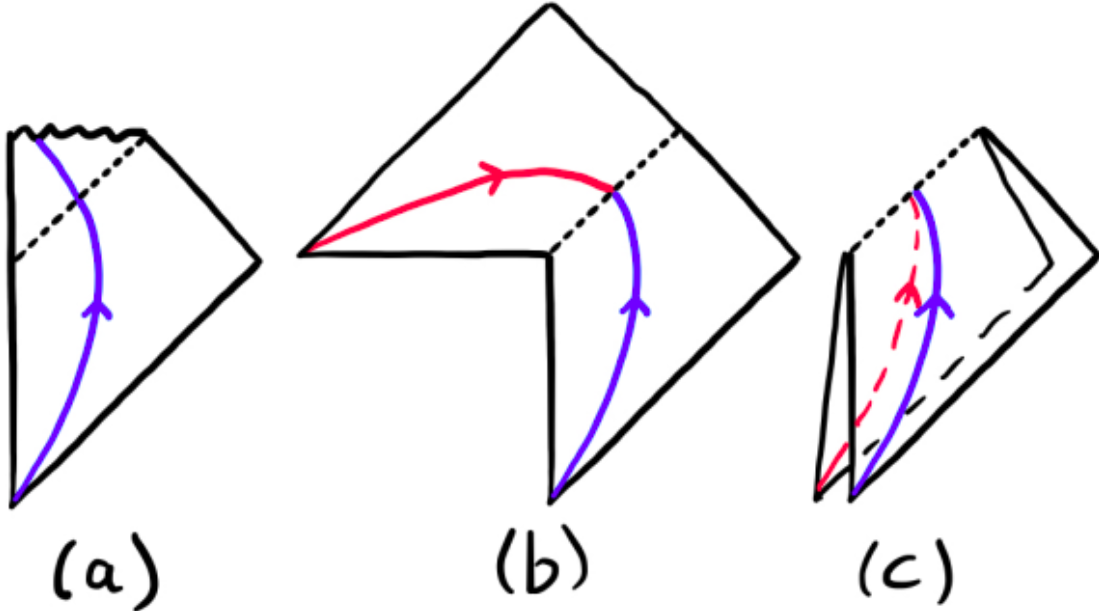
\includegraphics[width=0.65\textwidth]{parts/part2/figures/annihilate_BHmirror.png}
     \caption{In the black hole mirror model, the event horizon acts as a $CPT$-symmetric mirror connecting the exterior of our universe to the exterior of anti-universe. Infalling matter from our universe annihilates with infalling antimatter from the anti-universe at the horizon. The KD-Majorana condition provides a fundamental explanation for why the universe and anti-universe must remain perfectly $CPT$-symmetric, even at quantum scales.}
     \label{fig:annihilate_BHmirror}
\end{figure}

One might ask what physically transpires immediately following this horizon annihilation. There are two primary hypothetical scenarios: upon annihilation, the infalling matter is either (1) converted into photons permanently bound to travel along the event horizon, and/or (2) converted into Hawking radiation that is immediately emitted back outward into both the universe and the anti-universe. Both scenarios, however, face unresolved theoretical challenges.

Scenario (1) is conceptually appealing because it links directly to Hawking's original macroscopic description, where all in-falling information is holographically encoded on the event horizon, thereby dictating the Bekenstein-Hawking entropy. However, the critical challenge facing this scenario is that the presence of high-energy photons on the event horizon results in a non-zero energy-momentum tensor exactly at the boundary. This boundary is therefore no longer a true vacuum, which fundamentally violates the foundational mathematical assumptions of the purely vacuum Schwarzschild metric. Obtaining a mathematically consistent metric solution that accommodates this boundary energy likely requires complex numerical gravity treatments.

Scenario (2) postulates that the photons produced by the annihilation immediately escape as observable Hawking radiation. This scenario is highly attractive because it trivially resolves the black hole information loss paradox: the outgoing Hawking radiation is deterministically constructed from, and thus fully encodes the information of, the infalling particles. A conceptually similar framework was proposed by Gerard 't Hooft in 2025 (\cite{’tHooft2025}) to resolve the information paradox. In 't Hooft's model, the problematic black hole interior is mathematically replaced by a quantum clone of the exterior universe. The horizon acts as a "hard" mirror due to the Shapiro effect: an ingoing particle perturbatively modifies the local metric, generating a gravitational drag on outgoing particles. Consequently, the position and phase of the outgoing Hawking radiation are strictly determined by the momentum of the ingoing matter. Information simply bounces back out (from the reference frame of a distant external observer), meaning unitarity is trivially conserved. 

't Hooft's proposal differs crucially from Boyle's. 't Hooft deduced that the clone universe should be entirely identical to ours, albeit with time reversal; however, the precise physical ontology of this clone universe remained conceptually ambiguous. By assuming that external observers might theoretically detect particles emerging from both the primary and the clone universes, the 't Hooft model predicts a Hawking temperature twice the standard value, $T = 1/4\pi GM$. Conversely, in Boyle's proposal, the clone universe is explicitly identified as the unobservable $CPT$-reversed anti-universe. Because we cannot observe radiation emitted into the anti-universe, the detected Hawking radiation remains at the standard value, $T = 1/8\pi GM$. Despite these differences, the underlying logic for preserving information is remarkably similar. 

However, Scenario (2) also faces severe physical challenges. Primarily, these mirror models describe purely static black holes, leaving the mechanism of black hole growth unexplained. If all infalling matter effectively bounces back outward as Hawking radiation, how does a black hole ever accrue mass? Addressing this question naturally leads to another: if Hawking radiation is generated directly by infalling particles (analogous to localized flashes of light emanating from the horizon), how does the radiation acquire its perfectly thermalized spectrum? Standard Hawking radiation depends exclusively on the global mass of the black hole, not on the specific microstates of the infalling matter. 

To resolve this, we can turn to 't Hooft's explanation of the Shapiro effect. Locally, an infalling particle perturbs the metric, which directly dictates the phase of the emitted particles (or, in Boyle's framework, determines the kinematics of the localized annihilation event). However, both the ingoing and outgoing trajectories are overwhelmingly dominated by the global gravitational well of the black hole. This global metric governs the overarching spectrum of the Hawking radiation, seamlessly encoding the macroscopic mass of the black hole. Meanwhile, the specific quantum information of the infalling particles is encoded strictly in the localized metric perturbations—a sub-dominant, second-order effect. Therefore, macroscopic observations yield a perfectly thermalized spectrum, whereas a microscopic analysis of individual emitted particles could, in principle, trace the state back to the original infalling matter. One can hypothesize that due to this complex gravitational back-reaction, the outgoing Hawking radiation might carry slightly less total kinetic energy than the original infalling particles. This energy deficit would remain gravitationally bound at the horizon, thereby allowing the black hole to dynamically grow.

% Beyond cosmology, a forthcoming companion paper \cite{BoyleVaibhav} will demonstrate how KD fermions offer a radically new approach (building upon \cite{Catterall:2022jky, Catterall:2023nww}) for placing chiral gauge theories, such as the Standard Model, directly onto a lattice. We will discuss this lattice implementation in detail in the final chapter \cref{chapter:Conclusion_FutureWork}.
 
% Moreover, the profound geometric symmetries of the Lorentzian KD action described above suggest a natural and compelling interpretation within the framework of twistor space \cite{Penrose:1985bww, Penrose:1986ca, adamo2018lecturestwistortheory}, an avenue we strongly intend to explore. It is also worth explicitly noting the proposed connection between twistor space and the Standard Model outlined in \cite{woit2021euclideantwistorunification}, which exhibits promising parallels to the framework derived here. These geometric extensions will also be investigated in future work.

\printbibliography[heading=subbibintoc, title={References for Chapter \thechapter}]
\chapter{Euclidean Signature and Alternative Lagrangians}\label{chapter:Lag_Euclidean}

\chapterabstract{In this chapter, we first review the Hermiticity and chirality problems inherent to conventional Euclidean Lagrangians. We then introduce von Nieuwenhuizen's Wick rotation; by actively Wick rotating the spinors alongside the spacetime coordinates, the resulting Euclidean Lagrangian preserves the mathematical structure of its Lorentzian counterpart, successfully restoring Hermiticity. Unfortunately, this framework leaves the chirality problem unresolved. We subsequently extend this Wick rotation methodology to Kähler-Dirac (KD) fermions. Remarkably, due to the presence of the additional $\gamma^0$ matrix, chirality is strictly preserved in the Euclidean KD Lagrangian. This critical mathematical feature establishes a robust pathway for constructing anomaly-free chiral gauge theories on a lattice. Inspired by this Euclidean formulation, we also explore alternative configurations for the Lorentzian Lagrangian, rigorously analyzing their respective equations of motion, quantization properties, and associated KD-Majorana conditions. Our results demonstrate that, despite distinct mathematical expressions, the underlying physical paradigms—specifically the emergence of negative-norm states, the fundamental necessity of a two-sheeted spacetime, and the role of the KD-Majorana condition—remain fundamentally invariant.}

% 4. Possible solutions to Lagrangian in Euclidean signature: 
% - Conventional Euclidean Lagrangian: Hermitian problem, and chiral problem.
% - Question: could we solve the problem by direct Wick rotate Lagrangian in Lorentzian signature to Euclidean one? 
% - First try -- starting from SO(p,q), could we find a larger group which contain Wick rotation? The answer is no.
% - Solution: Van Nieuwenhuizen's Wick rotate conventional Dirac Lagrangian, get a Hermitian Lagrangian. However Chiral problem remain.
% - Solution: Nieuwenhuizen's Wick rotate KD fermions. It is Hermitian and Chiral! 
% - Barrett work about needing two sheets of Hilbert space to get the Chiral Lagrangian. We show a more elegant picture by our KD-Majorana fermion.
% - Different Lagrangians: with $\gamma^5$ acting from left/right/both sides. Discuss the Majorana and Dirac type Lagrangians, and the new eom (with additional $\gamma^5$ acting from the right of mass term).

% Editor's note: Elevated the introduction to sound more formal and academically rigorous.
The conventional Euclidean Lagrangian for Dirac fermions is given by: 
\[
\mathcal{L}_E=\psi^\dagger (\gamma_E^\mu\partial_\mu +m)\psi
\]
where $\gamma^\mu\partial_\mu$ is summed over $\mu=\{1,2,3,4\}$, with $\gamma^4=i\gamma^0$. 

It is straightforward to verify that this Lagrangian is inherently non-Hermitian: 
\[
\mathcal{L}_E^\dagger=\partial_\mu\psi^\dagger (\gamma_E^\mu)^\dagger \psi+m\psi^\dagger\psi=\psi^\dagger (-\gamma_E^\mu\partial_\mu +m)\psi
\]
Here, we have used the Euclidean signature property $(\gamma_E^\mu)^\dagger=\gamma_E^\mu$, and the minus sign in the kinetic term arises from integration by parts.

Furthermore, this standard Euclidean Lagrangian is non-chiral, since the kinetic term has left- and right-handed Weyl spinors coupled together. In other words, left- and right-handed spinors do not evolve independently, violating the observation. One might argue that possessing a non-Hermitian and non-chiral Lagrangian in Euclidean space is acceptable, provided that the physical properties evaluated in the Lorentzian signature remain robust. In this view, the Euclidean signature is merely a mathematical artifice: one Wick rotates to Euclidean space to perform the path integral, and subsequently rotates back to Lorentzian space to extract physical observables.

However, a fundamental difficulty arises because the Dirac Lagrangians in Lorentzian and Euclidean signatures cannot be continuously transformed into one another. Specifically, the Lorentzian kinetic term contains an additional $\gamma^0$ matrix, which has no direct analogue (i.e., no corresponding $\gamma_E^4$ insertion) in the standard Euclidean formulation. This structural discontinuity complicates the process of Wick rotating the Euclidean results back to the Lorentzian regime. It is precisely this discontinuity that renders the Euclidean Lagrangian non-Hermitian and non-chiral, even though its Lorentzian counterpart is both Hermitian and chiral. This suggests a potential resolution: if one can formulate a truly continuous Wick rotation, it may be possible to construct a Euclidean Lagrangian that fully inherits the physical properties of the Lorentzian one. 

Fortunately, this concept was explored in von Nieuwenhuizen's work \cite{VANNIEUWENHUIZEN199629}, leading to the discovery of a strictly Hermitian Euclidean Lagrangian (\cref{sec:Nieuwenhuizen_Wick_rotation}). However, while this Lagrangian resolves the Hermiticity issue, it remains non-chiral. Interestingly, by extending this continuous rotation formalism to Kähler-Dirac (KD) fermions, we can successfully construct a Lagrangian that is simultaneously Hermitian and chiral (\cref{sec:extend_KD}). Finally, motivated by these geometric properties, we demonstrate that there are multiple valid Lagrangian formulations in Lorentzian signature. We explore their properties and physical significance in \cref{sec:diff_Lagrangian}.

\section{van Nieuwenhuizen's Wick Rotation for the Standard Dirac Lagrangian}\label{sec:Nieuwenhuizen_Wick_rotation}

% Editor's note: Replaced conversational transitions and tightened mathematical prose.
Note that in this chapter, we assume $(-,+,+,+)$ metric convention, such that one only needs to Wick rotate time while keeping the three spatial coordinate invariant. Under this convention, the Dirac Lagrangian in Minkowski space is written as: 
\[
\mathcal{L}_M=-\psi^\dagger \gamma^0 i (\gamma^\mu\partial_\mu +m)\psi
\]
A standard Wick rotation maps real time to imaginary time via $t\to -i t_E$ and sets $\gamma^4=i\gamma^0$. The Lagrangian then becomes:
\[
\mathcal{L}_M=-\psi^\dagger \gamma^4(\gamma^\mu\partial_\mu +m)\psi
\]
where the sum over $\mu$ now runs from $1$ to $4$, and $\partial_t=i\partial_{t_E}\equiv i\partial_4$ (the additional $i$ cancel out the $i$ in kinetic term). 

Von Nieuwenhuizen's critical insight was that the Wick rotation must act not only on the spacetime coordinates, but also continuously on the spinors within a 5D rotational space, defining $\gamma^5=\gamma^1\gamma^2\gamma^3\gamma^4$. To achieve this, the spinor is rotated via $\psi_E =S(\theta=\pi/2)\psi$, where the rotation operator is $S(\theta)=e^{\gamma^4\gamma^5\theta}$. At $\theta=\pi/2$, the rotation maps the system fully into Euclidean signature. To ensure the resulting Euclidean Lagrangian is Hermitian, the conjugate field must transform as $\bar\psi_E =\bar\psi S^{-1}=\psi^\dagger\gamma^4 S^{-1}$. Since the matrices satisfy $S\gamma^4=\gamma^4 S^{-1}$, we find $\psi_E^\dagger \gamma^4 =\psi^\dagger S\gamma^4$, which simplifies to $\psi_E^\dagger=\psi^\dagger S$.

It is essential to emphasize that the Hermitian conjugate transforms as $\psi^\dagger \to \psi^\dagger S$, rather than $\psi^\dagger \to \psi^\dagger S^{-1}$ (noting that $S^T=S^\dagger =S^{-1}$). This distinction is required to enforce the correct transformation rule $\bar\psi\to \bar\psi S^{-1}$. Fortunately, this property is naturally satisfied since $\bar{\psi}=\psi^\dagger\gamma^4$ and $S\gamma^4=\gamma^4 S^{-1}$, .

Furthermore, the gamma matrices themselves must undergo the corresponding similarity transformation, $\gamma_E^\mu=S\gamma^\mu S^{-1}$:
\[\gamma_E^i=\gamma^i, \gamma_E^4=\gamma^4\cos\theta+\gamma^5\sin\theta=\gamma^5\text{ (when }\theta=\pi/2\text{)}, \\ \gamma_E^5=\gamma_E^1\gamma_E^2\gamma_E^3\gamma_E^4=-\gamma^4\]
, where $\gamma^i$ remain unchanged for $i=1,2,3$, while $\gamma^4$ and $\gamma^5$ swap roles. 
Combining these elements, we can Wick rotate the Lorentzian Lagrangian to obtain the Euclidean counterpart:
\begin{equation}
\begin{aligned}
\mathcal{L}_M  = -\psi^\dagger \gamma^4(\gamma^\mu\partial_\mu +m)\psi
&=-\psi^\dagger S\gamma^4(S\gamma^\mu S^{-1}\partial_\mu +m) S\psi\\
&=\psi_E^\dagger \textcolor{red}{\gamma_E^5}(\gamma_E^\mu\partial_\mu +m)\psi_E==\mathcal{L}_E
\end{aligned}
\end{equation}
where we have applied the identity $S\gamma^4=\gamma^4 S^{-1}$. Note that after the 5D Wick rotation, the $\gamma^4$ matrix in the Lorentzian Lagrangian is replaced by $\gamma_E^5$ in the Euclidean Lagrangian (while the one in $\gamma_E^\mu$ still remain $\gamma_E^4$). This additional $\gamma_E^5$ insertion is crucial for ensuring that the Euclidean Lagrangian is Hermitian, as we will demonstrate below.

We can readily confirm that this modified Lagrangian is Hermitian:
\[\mathcal{L}_E^\dagger= \partial_\mu\psi_E^\dagger(\gamma_E^\mu)^\dagger(\gamma_E^5)^\dagger\psi_E=-\psi_E^\dagger\gamma_E^\mu \gamma_E^5\partial_\mu\psi_E =\psi_E^\dagger \gamma_E^5\gamma_E^\mu\partial_\mu\psi_E=\mathcal{L}_E\]
Here, the minus sign arising from the anticommutation relation $\gamma_E^\mu\gamma_E^5=-\gamma_E^5\gamma_E^\mu$ perfectly cancels the minus sign generated by integration by parts.

% If we choose the Weyl basis, where $\gamma_E^\mu=\begin{pmatrix}0&\sigma^\mu\\ \bar\sigma^\mu &0\end{pmatrix}$ and $\gamma_E^5=\begin{pmatrix}\mathbbm{1}&0\\ 0&-\mathbbm{1}\end{pmatrix}$, we find that the Lorentz transformations for the left- and right-handed spinors remain decoupled:
% \begin{equation}
% \begin{aligned}
% \psi_E^\dagger \gamma_E^5\gamma_E^\mu\partial_\mu \psi_E &\to \psi_E^\dagger U_\Lambda^\dagger \gamma_E^5 U_\Lambda\gamma_E^\mu U_\Lambda^{-1}U_\Lambda\partial_\mu \psi_E\\
% \to U_\Lambda^\dagger \gamma_E^5 U_\Lambda=\gamma_E^5 &\text{, given }U_\Lambda=\begin{pmatrix}u_L&0\\ 0&u_R\end{pmatrix}\to u_L^\dagger u_L=u_R^\dagger u_R=\mathbbm{1}
% \end{aligned}
% \end{equation}
% Consequently, the system still preserves the required $SO(4)\sim SU(2)\times SU(2)$ Euclidean rotational symmetry. 

% Editor's note: Fixed "swap with roll" to "swap roles".
Despite these successes, this Lagrangian remains non-chiral. To illustrate this, consider the standard Weyl basis where $\gamma^\mu=i\begin{pmatrix}0& \sigma^\mu\\ -\sigma^\mu & 0\end{pmatrix}$ and $\gamma^5=\begin{pmatrix}\mathbbm{1}& 0\\ 0 & \mathbbm{1}\end{pmatrix}$ \footnote{In this chapter, we choose (-+++) convention, where $\gamma^i=i\begin{pmatrix}0& \sigma^i\\ -\sigma^i & 0\end{pmatrix}, \gamma^0=\begin{pmatrix}0& \mathbbm{1}\\ -\mathbbm{1} & 0\end{pmatrix}$, and $\gamma^4=i\gamma^0$. Here the index $\mu$ runs from 1 to 4, so $\gamma^\mu=i\begin{pmatrix}0& \sigma^\mu\\ -\sigma^\mu & 0\end{pmatrix}$. The corresponding $\gamma^5=\gamma^1\gamma^2\gamma^3\gamma^4=\begin{pmatrix}\mathbbm{1}& 0\\ 0 & \mathbbm{1}\end{pmatrix}$}. After the Wick rotation, $\gamma^4$ and $\gamma^5$ swap roles; consequently, $\gamma^4_E$ becomes diagonal while $\gamma_E^5$ becomes off-diagonal. As a result, the time derivative term in $\psi_E^\dagger \gamma_E^5(\gamma_E^\mu\partial_\mu +m)\psi_E$ inevitably mixes chiralities. Interestingly, this chirality problem is naturally resolved when we transition to the Kähler-Dirac fermion framework.


\section{Extension to the KD Lagrangian}\label{sec:extend_KD}


The Minkowski Lagrangian for KD fermions is given by: 
\[
\mathcal{L}_M=-\,{\rm Tr}[\gamma^0\Psi^\dagger \gamma^0 i (\gamma^\mu\partial_\mu +m)\Psi]
\]
Note that $\Psi$ is a $4\times 4$ bi-spinor matrix. To ensure that the bilinear $\bar\Psi\Psi$ is Lorentz invariant, an additional $\gamma^0$ must act from the left, defining the adjoint as $\bar{\Psi}=\gamma^0\Psi^\dagger \gamma^0$. We can diagonalize this additional $\gamma^0$ matrix via $\gamma^0=\Omega \Lambda\Omega^T$, where $\Lambda=-\gamma^5$. By absorbing the rotation matrix $\Omega$ into a redefined field, $\Psi'=\Psi\Omega$, the Lagrangian takes the form: 
\[
\mathcal{L}_M=-\,{\rm Tr}[\gamma^5\Psi'^\dagger \gamma^0 i (\gamma^\mu\partial_\mu +m)\Psi']
\]
Following the exact same Wick rotation methodology as in the previous section (where $\Psi_E=S\Psi S^{-1}$ and $\Psi_E^\dagger=S^{-1}\Psi^\dagger S$), the corresponding Euclidean Lagrangian evaluates to:
\begin{equation}\label{eq:Euclidean_KD_Lagrangian}
    \mathcal{L}_E=\,{\rm Tr}[\gamma_E^4\Psi_E^\dagger \gamma_E^5(\gamma_E^\mu\partial_\mu +m)\Psi_E]
\end{equation}

% Editor's note: Changed \psi_E to \Psi_E in the trace equations to maintain consistency with the bi-spinor notation used in this section.
We can immediately verify that this Lagrangian is Hermitian: 
\[\mathcal{L}_E^\dagger=\,{\rm Tr}[ \partial_\mu\Psi_E^\dagger(\gamma_E^\mu)^\dagger(\gamma_E^5)^\dagger\Psi_E(\gamma_E^4)^\dagger]=-\,{\rm Tr}[\Psi_E^\dagger\gamma_E^\mu \gamma_E^5\partial_\mu\Psi_E \gamma_E^4]=\,{\rm Tr}[\gamma_E^4\Psi_E^\dagger \gamma_E^5\gamma_E^\mu\partial_\mu\Psi_E]=\mathcal{L}_E\]
where we utilized the cyclic property of the trace, $\,{\rm Tr}[ABC]=\,{\rm Tr}[CAB]$.

% By following a calculation identical to that in the previous section, one can also confirm that this formulation rigorously preserves the $SO(4)=SU(2)\times SU(2)$ symmetry.

Most importantly, we can prove that this KD Euclidean Lagrangian is strictly chiral when evaluated in the Weyl basis, where $\gamma_E^\mu$ are off-diagonal $\gamma_E^\mu=i\begin{pmatrix}0& \sigma^\mu\\ -\sigma^\mu & 0\end{pmatrix}$ and $\gamma_E^5=\begin{pmatrix}\mathbbm{1}& 0\\ 0 & \mathbbm{1}\end{pmatrix}$:
\begin{equation}\label{eq:Lagrangian_KD_Euclidean}
\begin{aligned}
    \mathcal{L}_E&=\,{\rm Tr}[\gamma_E^4\Psi_E^\dagger \gamma_E^5\gamma_E^\mu\partial_\mu \Psi_E]\\
    &=-\,{\rm Tr}\left[\begin{pmatrix}0& \mathbbm{1}\\ -\mathbbm{1} & 0\end{pmatrix}(\Psi_{E,+}^\dagger+\Psi_{E,-}^\dagger )\begin{pmatrix}\mathbbm{1}& 0\\ 0 & \mathbbm{1}\end{pmatrix}\begin{pmatrix}0& \sigma^\mu\\ -\sigma^\mu & 0\end{pmatrix}(\partial_\mu \Psi_{E,+}+\partial_\mu \Psi_{E,-})\right]\\
    &=-\left(\,{\rm Tr}[\gamma_E^4\Psi_{E,+}^\dagger \gamma_E^5\gamma_E^\mu\partial_\mu \Psi_{E,+}]+\,{\rm Tr}[\gamma_E^4\Psi_{E,-}^\dagger \gamma_E^5\gamma_E^\mu\partial_\mu \Psi_{E,-}]\right)\\
    &=\,{\rm Tr}[(\ell_L^c)^\dagger\sigma^\mu\partial_\mu\ell_L]+\,{\rm Tr}[(\ell_R^c)^\dagger\sigma^\mu\partial_\mu\ell_R]-\text{h.c.}
\end{aligned}
\end{equation}
In this derivation, we applied the KD-Majorana condition: 
$\Psi=\begin{pmatrix}
        \ell_L& \ell_R^c \\
        \ell_R& \ell_L^c
    \end{pmatrix}=\Psi^c$
and separated $\Psi$ into its block-diagonal ($\Psi_+$) and block-off-diagonal ($\Psi_-$) components as follows:
\begin{equation}
\begin{aligned}
   \Psi_{\pm}=\frac{1}{2}(\Psi\pm\gamma^5\Psi\gamma^5) \quad \implies \quad \Psi_+=\begin{pmatrix}
        \ell_L& 0 \\
        0& \ell_L^c
    \end{pmatrix}, \quad \Psi_-=\begin{pmatrix}
        0& \ell_R^c \\
        \ell_R& 0
    \end{pmatrix}
\end{aligned}
\end{equation}

The final expression in \cref{eq:Lagrangian_KD_Euclidean} demonstrates that the Weyl spinor natively couples with its own charge conjugate, where LH and RH fermions are decoupled -- it is a chiral theory! Moreover, this outcome aligns perfectly with the recent theoretical results published by Barrett \cite{Barrett2024}. Barrett established that a strictly chiral theory mandates a spacetime dimension of $2 \text{ mod } 8$ (e.g., $2, 10, 18, \dots$). However, physical spacetime is 4-dimensional. To resolve this apparent contradiction, Barrett demonstrated that a chiral model can be successfully constructed in 4D by doubling the Hilbert space (effectively utilizing a two-sheeted 4D spacetime), formulated mathematically as $\langle J\psi|D\psi\rangle$, where $J\psi=\psi^c$. This is remarkably consistent with our derived \cref{eq:Lagrangian_KD_Euclidean}, which explicitly features particles coupled to their corresponding antiparticles.

This result carries significant theoretical weight. In a forthcoming paper \cite{BoyleVaibhav}, Vaibhav and Boyle apply Barrett's argument by positing a doubled Hilbert space (two distinct 4D spacetimes and two independent KD fields) to construct an anomaly-free KD lattice gauge theory. However, the derivation presented here reveals that this two-sheeted spacetime structure is already intrinsically encoded within the fundamental geometry of a \textit{single} KD field (as evidenced by \cref{eq:Lagrangian_KD_Euclidean}). We do not need to introduce a second independent KD field to achieve this doubling. 

Why, then, should we utilize KD fields for lattice gauge theory? The original motivation was that KD fields can be seamlessly mapped onto differential forms, allowing them to be discretized on a lattice without introducing unphysical fermion doubling. We now have a profound secondary motivation: the geometric requirement of a two-sheeted 4D spacetime—necessary to resolve the chiral anomaly—is naturally and elegantly embedded within the structure of a single KD field. This makes the KD formalism a uniquely powerful candidate for constructing anomaly-free lattice gauge theories.

A final subtlety regarding the Wick rotation should be noted. During the rotation, we effectively swap $\gamma^4_E \leftrightarrow \gamma_E^5$. In Lorentzian signature, this corresponds to swapping $\gamma^0 \leftrightarrow \gamma^5$, which is equivalent to transforming between the Weyl and Dirac bases. Consequently, if one begins in Lorentzian signature using the Weyl basis, the standard Wick rotation yields a Euclidean Lagrangian cast in the Dirac basis—a formulation that obfuscates the underlying chiral properties. However, because a change of basis (Weyl vs. Dirac) leaves the underlying physics invariant, we are free to apply a basis transformation immediately after the Wick rotation to ensure the Lagrangian remains explicitly chiral in both signatures. This basis change does not affect the physical observables derived from the path integral. The invariance is easily proven:
\begin{equation}
\begin{aligned}
    \gamma^\mu\to S\gamma^\mu S^{-1}, \quad \psi\to S\psi , \quad \psi^\dagger\to \psi^\dagger S^\dagger\\
    \psi^\dagger \gamma^0\gamma^\mu\partial_\mu \psi\to \psi^\dagger S^\dagger S\gamma^0 S^{-1} S\gamma^\mu S^{-1}S\partial_\mu \psi=\psi^\dagger \gamma^0\gamma^\mu\partial_\mu \psi
\end{aligned}
\end{equation}

Having established a continuous Wick rotation that maps the Lagrangian into a well-defined Euclidean signature, the next technical challenge is performing the Euclidean path integral via the new Hermitian and chiral Lagrangian, and subsequently Wick rotating back to compute exact physical probability amplitudes. This extensive calculation is left for future work.


\section{Alternative Lagrangians}\label{sec:diff_Lagrangian}

Examining the Euclidean KD Lagrangian in \cref{eq:Euclidean_KD_Lagrangian}, we note the critical presence of the additional $\gamma_E^5$ matrix. Returning to Lorentzian signature, recall that the existence of negative-norm (ghost) states in the KD field stems directly from the additional $\gamma^0$ in the Lagrangian's kinetic term. This raises an intriguing theoretical question: is it possible to define an alternative Lorentzian Lagrangian by judiciously inserting $\gamma^5$ operators such that the negative-norm states are entirely eliminated? Note that multiplying the original Lagrangian $\mathcal{L}_M={\rm Tr}[\gamma^0 \Psi^\dagger \gamma^0\gamma^\mu\partial_\mu\Psi]$ by $\gamma^5$ remains theoretically viable; because $\gamma^5$ anticommutes with $\gamma^\mu$, the action remains fully Lorentz invariant.

At first glance, this approach appears highly promising. After diagonalizing the extra $\gamma^0$, the Lagrangian takes the form $\mathcal{L}_M={\rm Tr}[\Lambda \Psi'^\dagger \gamma^0\gamma^\mu\partial_\mu\Psi']$, where $\Lambda=-\gamma^5$. Since $(\gamma^5)^2=\mathbbm{1}$, it seems that multiplying the action by an additional $\gamma^5$ would perfectly cancel the negative signs, rendering the entire theory positive-definite. 

However, this naive approach overlooks the necessary transformation of the matrices themselves. Recall that we diagonalized $\gamma^0$ via $\gamma^0=\Omega \Lambda\Omega^\top=-\Omega \gamma^5\Omega^\top$. Under this same transformation matrix $\Omega$, $\gamma^5$ itself transforms into $\gamma^5=\Omega\gamma^0\Omega^\top$. Consequently, any new Lagrangian featuring an explicitly inserted $\gamma^5$ will invariably introduce a transformed $\gamma^0$ matrix, ensuring that the problematic negative-norm states persist. 

\begin{equation}
\begin{aligned}
    \mathcal{L}_M&={\rm Tr}[\gamma^5\gamma^0 \Psi^\dagger \gamma^0\gamma^\mu\partial_\mu\Psi]
    =-{\rm Tr}[(\Omega \gamma^0\Omega^\top)(\Omega \gamma^5\Omega^\top)\Psi^\dagger \gamma^0\gamma^\mu\partial_\mu\Psi]\\
    &=-{\rm Tr}[\gamma^0\gamma^5(\Psi\Omega)^\dagger\gamma^0\gamma^\mu\partial_\mu(\Psi\Omega)]
    =-{\rm Tr}[\gamma^0\gamma^5\Psi'^\dagger\gamma^0\gamma^\mu\partial_\mu \Psi']
\end{aligned}
\end{equation}

One might suggest inserting the $\gamma^5$ directly into the \textbf{already-transformed} Lagrangian. However, this brutally violates Lorentz invariance. The transformed field $\Psi'=\Psi\Omega$ obeys the modified Lorentz transformation $\Psi'\to U_\Lambda \Psi' U_\Lambda'^{-1}$, where $U_\Lambda'$ is the standard Lorentz matrix with its $\gamma^0$ generators replaced by $\gamma^5$ (as discussed in \cref{subsec:mixing_term_Lorentz_spin_connection}). For reader's convenience, I write it explicitly again:

\begin{equation}
\begin{aligned}
    &\Psi\to U_\Lambda \Psi U_\Lambda^{-1}
    , \quad \Psi'=\Psi\Omega \\
    \implies & U_\Lambda \Psi U_\Lambda^{-1}\Omega =U_\Lambda \Psi \Omega \Omega^{-1}U_\Lambda^{-1} \Omega=U_\Lambda \Psi' U_\Lambda'^{-1}
\end{aligned}
\end{equation}
where $U_\Lambda'^{-1}=\Omega^{-1}U_\Lambda^{-1} \Omega$.
Because $\Omega^{-1}\gamma^0 \Omega=-\gamma^5$ and $\Omega^{-1}\gamma^i \Omega=\gamma^i$, $U_\Lambda'$ is structurally identical to a Lorentz transformation matrix wherein $\gamma^0$ is mapped to $\gamma^5$. Specifically, if $U_\Lambda$ is defined in the Weyl basis, $U_\Lambda'$ evaluates equivalently to a transformation in the Dirac basis.

Therefore, manually appending a $\gamma^5$ matrix from the left (of \textbf{already-transformed} Lagrangian) to explicitly cancel the negative-norm states (i.e. $\Lambda=-\gamma^5$ from diagonalized $\gamma^0$) fundamentally destroys the Lorentz invariance of the theory.

Although it is strictly impossible to mathematically eliminate the negative-norm states by redefining $\bar\Psi$ with extra $\gamma^5$ insertions, these variant Lagrangians remain mathematically valid Lorentz-invariant formulations. In the remainder of this section, we explore the properties and physical implications of appending $\gamma^5$ from the left, right, or both sides of the spinor. 

First, we establish their geometric connection to differential forms. By selecting the off-diagonal Weyl basis $\gamma^\mu=\begin{pmatrix}
    0& \sigma^\mu \\ \bar\sigma^\mu &0
\end{pmatrix}$, the $4\times 4$ KD spinor maps to differential forms as $\Psi=\begin{pmatrix}
    E& O' \\ O &E'
\end{pmatrix}$, where the diagonal and off-diagonal blocks explicitly correspond to even ($E$) and odd ($O$) forms, respectively. Multiplying by $\gamma^5$ from both sides strategically applies a minus sign exclusively to the off-diagonal (odd-form) blocks: $\gamma^5\Psi\gamma^5=\begin{pmatrix}
    E& -O' \\ -O &E'
\end{pmatrix}$. Consequently, defining a Lorentz-invariant bilinear $\bar{\Psi}\Psi$ by appending $\gamma^5$ to both sides of the adjoint is functionally equivalent to flipping the sign of the odd-form kinetic terms. This variant elegantly preserves a transparent mapping to the underlying exterior calculus. In contrast, appending a single $\gamma^5$ from either the left or the right obscures this geometric mapping. Nevertheless, we will rigorously evaluate all configurations as theoretically viable spinor formulations.


\subsection{Construction of Hermitian and Physical Lagrangians}

A physically viable Lagrangian must be strictly Hermitian, and its variation must systematically recover a generalized Klein-Gordon equation. When inserting $\gamma^5$ operators on the left, right, or both sides of the adjoint $\bar\Psi$, one frequently discovers that the kinetic trace ${\rm Tr}[i\bar{\Psi}\gamma^\mu\partial_\mu\Psi]$ or the mass trace ${\rm Tr}[m\bar{\Psi}\Psi]$ becomes anti-Hermitian. While it is tempting to simply multiply the offending term by an imaginary unit "$i$" to restore Hermiticity, this naive fix often destroys the correct Klein-Gordon equation of motion. A strictly physical Lagrangian must carefully satisfy both requirements.

We categorize the permissible physical Lagrangians below. 
When $\gamma^5$ acts exclusively from the left, both the kinetic and mass terms naturally evaluate as anti-Hermitian. Consequently, we multiply both terms by "$i$": 
\begin{equation}
    \mathcal{L}_1={\rm Tr}[ \bar\Psi\gamma^\mu\partial_\mu\Psi+im\bar\Psi\Psi], \quad \text{where } \bar\Psi=\gamma^5\gamma^0\Psi^\dagger\gamma^0
\end{equation}

This modifying "$i$" subsequently propagates into the derived equation of motion. The resulting Klein-Gordon equation acquires an overall minus sign from $i^2=-1$, but the fundamental dynamical relationship $\partial^2 + m^2 = 0$ is preserved perfectly.

When $\gamma^5$ acts from the right (or from both sides), the Hermiticity mismatch is split: only one of the two terms (kinetic or mass) evaluates as anti-Hermitian. Multiplying only the anti-Hermitian term by "$i$" introduces a relative sign error, generating a tachyonic or ill-defined Klein-Gordon equation. To resolve this, we must construct hybridized Lagrangians that systematically mix the right-acting and both-acting adjoint definitions: 
\begin{equation}
\begin{aligned}
    \mathcal{L}_2={\rm Tr}[ i\bar\Psi_{\text{right}}\gamma^\mu\partial_\mu\Psi-m\bar\Psi_{\text{both}}\Psi]; &\quad
    \mathcal{L}_3={\rm Tr}[ \bar\Psi_{\text{both}}\gamma^\mu\partial_\mu\Psi-im\bar\Psi_{\text{right}}\Psi], \\
    \text{where }\bar\Psi_{\text{right}}=\gamma^0\Psi^\dagger\gamma^0\gamma^5,&\qquad \bar\Psi_{\text{both}}=\gamma^5\gamma^0\Psi^\dagger\gamma^0\gamma^5.
\end{aligned}
\end{equation}
Because these hybrid Lagrangians feature mismatched powers of $\gamma^5$ across the kinetic and mass terms, their varied equation of motion takes the highly non-standard form: 
\begin{equation}
    i\gamma^\mu\partial_\mu\Psi -m\Psi\gamma^5=0
\end{equation}
which features an unusual $\gamma^5$ matrix acting on the mass term from the right \footnote{Because the additional $\gamma^5$ in the equation $i\gamma^\mu\partial_\mu\Psi-m\Psi\gamma^5=0$ effectively flips the sign of the latter two columns of $\Psi$, one might naively conclude that the fermions on the backward sheet possess negative inertial mass. This interpretation is incorrect. The true physical mass must be evaluated in the diagonalized basis $\Psi'=\Psi\Omega$. Take $\mathcal{L}_2$ for example, the diagonalized equation of motion becomes $i\gamma^\mu\partial_\mu\Psi'-m\Psi'\gamma^0=0$, wherein an additional $\gamma^0$ acts on the mass term. Because the diagonalized spinor itself is internally restructured as $\Psi'=\begin{pmatrix}\ell_L& \ell_R^c\\ \ell_L^c & \ell_R  \end{pmatrix}$ (will discussed in \cref{subsec:KD_Majorana_diff_Lagrangian}), expanding the matrix trace proves that the physical mass terms evaluate identically to those of the conventional Lagrangian.}. Astonishingly, this exotic equation of motion strictly satisfies the standard Klein-Gordon dynamics. This is proven by defining the independent kinetic and mass operators:
\[ D(\Psi)=i\gamma^\mu \partial_\mu\Psi,\quad M(\Psi)=m\Psi\gamma^5\]

Because these two operators fundamentally commute, $D(M(\Psi))=M(D(\Psi)) \implies [D,M]=0$, operating twice on the field yields: 
\begin{equation}
    (D+M)(D-M)\Psi=(D^2-M^2)\Psi=-(\partial^2+m^2)\Psi=0
\end{equation}
which is identically the required Klein-Gordon equation. Note that this unique dynamical property is exclusively permitted for $4\times 4$ KD spinors, as $4\times 1$ spinors could not  have matrix multiplied from the right-hand side (i.e. the additional $\gamma^5$).

The next critical step is to quantize these variant Lagrangians to definitively check for the presence of negative-norm states. To simplify this analysis, we employ the same diagonalization procedure used for the original Lagrangian ($\bar\Psi=\gamma^0\Psi^\dagger\gamma^0$), transforming the kinetic structure into a form resembling the conventional Dirac framework. 

For the left-acting Lagrangian $\mathcal{L}_1$, we diagonalize the combined matrix $\gamma^5\gamma^0$, yielding: 
\begin{equation}
\begin{aligned}
    \mathcal{L}_1&={\rm Tr}[ \gamma^5\gamma^0\Psi^\dagger\gamma^0\gamma^\mu\partial_\mu\Psi+im\gamma^5\gamma^0\Psi^\dagger\gamma^0\Psi]\\
    &={\rm Tr}[ i\gamma^5\Psi'^\dagger\gamma^0\gamma^\mu\partial_\mu\Psi'-m\gamma^5\Psi'^\dagger\gamma^0\Psi']
\end{aligned}
\end{equation}
where $\gamma^5\gamma^0=\Omega(\textcolor{red}{i}\gamma^5)\Omega^\dagger$ and $\Psi'=\Psi\Omega$. Note that the additional "$i$" in diagonalized matrix $i\gamma^5$ cancel out with the overall "$i$" previously added to make the Lagrangian Hermitian, causing the final trace perfectly mirrors the conventional KD Lagrangian.

Analyzing the hybrid Lagrangian $\mathcal{L}_2={\rm Tr}[ i\bar\Psi_{\text{right}}\gamma^\mu\partial_\mu\Psi-m\bar\Psi_{\text{both}}\Psi]$ is considerably more intricate. After diagonalizing the embedded $\gamma^0$, the kinetic term expands to: 

\begin{equation}
\begin{aligned}
    \mathcal{L}_2^{\text{kin}}&={\rm Tr}[ i\gamma^0\Psi^\dagger\gamma^0\gamma^5\gamma^\mu\partial_\mu\Psi]={\rm Tr}[ i(\gamma^5\Psi'^\dagger\gamma^5)\gamma^0\gamma^\mu\partial_\mu\Psi']\\
    &={\rm Tr}[ i(\Psi_+'^\dagger-\Psi_-'^\dagger)\gamma^0\gamma^\mu\partial_\mu(\Psi_+'+\Psi'_-)]\\
    &={\rm Tr}[ i\Psi_+'^\dagger\gamma^0\gamma^\mu\partial_\mu\Psi_+']-{\rm Tr}[ i\Psi_-'^\dagger\gamma^0\gamma^\mu\partial_\mu\Psi_-']
\end{aligned}
\end{equation}
where $\Psi'_\pm=\frac{1}{2}(\Psi'\pm\gamma^5\Psi'\gamma^5)$, which implies $\gamma^5\Psi'\gamma^5=\Psi'_+-\Psi'_-$. The components $\Psi'_+$ and $\Psi'_-$ represent the diagonal and off-diagonal blocks of the matrix field, respectively. 

Performing an identical decomposition for the mass term gives: 
\begin{equation}
    -m{\rm Tr}[ \gamma^5\gamma^0\Psi^\dagger\gamma^0\gamma^5\Psi]=-m{\rm Tr}[\gamma^0\Psi_+'^\dagger\gamma^0\Psi_+']+m{\rm Tr}[\gamma^0\Psi_-'^\dagger\gamma^0\Psi_-']
\end{equation}

In standard chiral gauge theories, the kinetic operators fully decouple the left- and right-handed spinors (e.g., $i\ell_L^\dagger\bar\sigma^\mu\partial_\mu\ell_L$), whereas the mass operator strongly couples them (e.g., $m\ell_L^\dagger\ell_R$). To satisfy this structural requirement, we are mathematically forced to define the internal matrix as $\Psi'=\begin{pmatrix} \ell_L&\ell_R^c\\ \ell_L^c & \ell_R\end{pmatrix}$. This configuration explicitly differs from the conventional definition, $\Psi'=\begin{pmatrix} \ell_L&\ell_R^c\\  \ell_R&\ell_L^c\end{pmatrix}$. Consequently, the required KD-Majorana condition must be heavily modified (as detailed in \cref{subsec:KD_Majorana_diff_Lagrangian}). Furthermore, because the Lagrangian for $\Psi'_-$ (the off-diagonal components) carries a leading minus sign, these specific components represent the physical fermions constrained to the backward spacetime sheet. 

Finally, we analyze the inverted hybrid Lagrangian $\mathcal{L}_3={\rm Tr}[ \bar\Psi_{\text{both}}\gamma^\mu\partial_\mu\Psi-im\bar\Psi_{\text{right}}\Psi]$. After diagonalizing the left-acting $\gamma^5\gamma^0$ matrix and separating the field into $\Psi_\pm$, the kinetic term evaluates to:
\begin{equation}
\begin{aligned}
    {\rm Tr}[ \gamma^5\gamma^0\Psi^\dagger\gamma^0\gamma^5\gamma^\mu\partial_\mu\Psi]=-{\rm Tr}[ i\Psi_+'^\dagger\gamma^0\gamma^\mu\partial_\mu\Psi_+']+{\rm Tr}[ i\Psi_-'^\dagger\gamma^0\gamma^\mu\partial_\mu\Psi_-']
\end{aligned}
\end{equation}
The requisite "$i$" emerges from the diagonalization $\gamma^5\gamma^0=\Omega(i\gamma^5)\Omega^\dagger$. Notice that this kinetic term structurally mirrors $\mathcal{L}_2$.

The mass term for $\mathcal{L}_3$ diagonalizes to: 
\begin{equation}
    {\rm Tr}[im\gamma^0\Psi'\gamma^0\gamma^5\Psi']
\end{equation}
To preserve algebraic consistency across the terms, we must employ the exact same transformation matrix $\Omega$ used above ($\gamma^5\gamma^0=\Omega(i\gamma^5)\Omega^\dagger$) to define $\Psi'=\Psi\Omega$. This constraint forces the lingering left-acting $\gamma^0$ to remain in the mass trace. 

The spurious "$i$" and $\gamma^5$ operators in this mass term can be beautifully canceled by executing a global chiral phase transformation, $\Psi'\to e^{i\frac{\pi}{4}\gamma^5}\Psi'$ (which leaves the kinetic term invariant). The mass term then collapses to: 
\begin{equation}
    {\rm Tr}[-m\gamma^0\Psi'\gamma^0\Psi']
\end{equation}

Recombining the simplified kinetic and mass blocks yields: 
\begin{equation}
    {\rm Tr}[-m\gamma^0\Psi'\gamma^0\Psi']=-m{\rm Tr}[\gamma^0\Psi_+'^\dagger\gamma^0\Psi_+']-m{\rm Tr}[\gamma^0\Psi_-'^\dagger\gamma^0\Psi_-']
\end{equation}
Crucially, the mass terms for $\Psi'_+$ and $\Psi'_-$ here carry identical signs. This parity differs from $\mathcal{L}_2$, distinguishing the two theories purely by their chiral structure. If one alternatively redefines the internal matrix as $\Psi'=\begin{pmatrix} \ell_L&-\ell_R^c\\ \ell_L^c & \ell_R\end{pmatrix}$ or $\begin{pmatrix} \ell_L&\ell_R^c\\ -\ell_L^c & \ell_R\end{pmatrix}$, the mathematical structure of $\mathcal{L}_3$ becomes entirely isomorphic to $\mathcal{L}_2$.

Throughout this rigorous analysis, we confirm that regardless of how $\gamma^5$ is inserted into the KD Lagrangian, exactly half of the dynamical terms acquire a negative sign. The fundamental topological necessity of the two-sheeted spacetime architecture is mathematically inescapable.

\subsection{The KD-Majorana Condition}\label{subsec:KD_Majorana_diff_Lagrangian}

We must now evaluate how the vital KD-Majorana condition is modified across these three Lagrangian variants, shedding light on their distinct physical interpretations. 

Recall that the canonical charge conjugation for KD fermions is defined as $\Psi^c=(i\gamma^2)\Psi^*(i\gamma^2)$. Upon diagonalizing the additional $\gamma^0$ and absorbing the transformation into $\Psi'=\Psi\Omega$, this condition maps cleanly into the new basis:
\[ \Psi'^c=(i\gamma^2)\Psi^*(i\gamma^2)\Omega=(i\gamma^2)(\Psi\Omega)^*\Omega^{-1}(i\gamma^2)\Omega=(i\gamma^2)\Psi'^*(i\gamma^2)\]
This simplification relies on the fact that $\Omega$ is purely real ($\Omega^*=\Omega=\frac{1}{\sqrt{2}}\begin{pmatrix} \mathbbm{1}&-\mathbbm{1}\\ \mathbbm{1}&\mathbbm{1} \end{pmatrix}$) and satisfies $\Omega^{-1}(i\gamma^2)\Omega=(i\gamma^2)$.

For the conventional Lagrangian, populating the field as $\Psi'=\begin{pmatrix}\ell_L& \ell_R^c\\ \ell_R & \ell_L^c  \end{pmatrix}$ ensures that $\Psi'^c=(i\gamma^2)\Psi'^*(i\gamma^2)=\Psi'$, explicitly satisfying the KD-Majorana condition. As detailed in the previous chapter, substituting this specific internal structure into the kinetic, mass, and Yukawa traces perfectly recovers the standard interactions of the SM. 

For the variant Lagrangian featuring a left-acting $\gamma^5$ ($\mathcal{L}_1$), the transformation matrix $\Omega$ evaluates as strictly imaginary ($\Omega=\frac{1}{\sqrt{2}}\begin{pmatrix} \mathbbm{1}&i\mathbbm{1}\\ i\mathbbm{1}&\mathbbm{1} \end{pmatrix}$), since the diagonalization targets $\gamma^5\gamma^0$ rather than $\gamma^0$. Despite this shift, one can rigorously prove that the identity $\Psi'^c=(i\gamma^2)\Psi'^*(i\gamma^2)$ remains valid. If we assume the conventional population $\Psi'=\begin{pmatrix}\ell_L& \ell_R^c\\ \ell_R & \ell_L^c  \end{pmatrix}$, we again successfully recover $\Psi'^c=\Psi'$. 

However, for the hybrid variants $\mathcal{L}_2$ and $\mathcal{L}_3$, the underlying Lagrangian structure diverges sharply from the conventional KD framework, necessitating a revised approach.

Consider $\mathcal{L}_2$. To successfully extract standard SM terms from this action (e.g., proper chiral kinetic terms and mixed LH/RH mass terms), we are forced to populate the matrix as $\Psi'=\begin{pmatrix}\ell_L& \ell_R^c\\ \ell_L^c & \ell_R  \end{pmatrix}$. Executing the charge conjugation operator on this specific block configuration yields: 
\[ \Psi'^c=(i\gamma^2)\begin{pmatrix}\ell_L& \ell_R^c\\ \ell_L^c & \ell_R  \end{pmatrix}^*(i\gamma^2)=\begin{pmatrix}-\ell_R^c& -\ell_L\\ \ell_R & \ell_L^c  \end{pmatrix}=\gamma^5\Psi'\gamma^0\]
This transformed field is explicitly not equal to $\Psi'$. However, this modified KD-Majorana condition ($\Psi'^c=\gamma^5\Psi'\gamma^0$) is nonetheless invariant under Lorentz transformations. Here is the proof:

The Lorentz transformation of the diagonalized field is governed by $U_\Lambda\Psi'U_\Lambda'$. Because $U_\Lambda$ is spanned by the standard basis $\gamma^\mu$ ($\mu=\{0,1,2,3\}$) while $U_\Lambda'$ is spanned by the alternate basis ($\mu=\{5,1,2,3\}$), the modified KD-Majorana condition remains invariant under the transformation: 
\[\tilde\Psi'^c=U_\Lambda\Psi'^cU_\Lambda'=U_\Lambda\gamma^5\Psi'\gamma^0U_\Lambda'=\gamma^5U_\Lambda\Psi'U_\Lambda'\gamma^0 =\gamma^5\tilde\Psi'^c\gamma^0\]
which relies on the standard commutation properties $[\gamma^5,U_\Lambda]=0$ and $[\gamma^0,U'_\Lambda]=0$.

An identical geometric consistency applies to $\mathcal{L}_3$. The baseline charge conjugation operator remains $\Psi'^c=(i\gamma^2)\Psi'^*(i\gamma^2)$. However, due to its requisite internal population $\Psi'=\begin{pmatrix}\ell_L& -\ell_R^c\\ \ell_L^c & \ell_R  \end{pmatrix}$, the emergent KD-Majorana condition evaluates to:
\[ \Psi'^c=(i\gamma^2)\begin{pmatrix}\ell_L& -\ell_R^c\\ \ell_L^c & \ell_R  \end{pmatrix}^*(i\gamma^2)=\begin{pmatrix}-\ell_R^c& -\ell_L\\ -\ell_R & \ell_L^c  \end{pmatrix}=\gamma^5\Psi'(\gamma^5\gamma^0)\]

This KD-Majorana condition is similarly Lorentz invariant. Under the transformation $U_\Lambda\Psi'U_\Lambda'$, the right-acting matrix $U_\Lambda'$ is constructed using the hybridized basis $\gamma^\mu$ where $\mu=\{50,1,2,3\}$, defining $\gamma^{50}=\gamma^5\gamma^0$. After applying the commutation relations between the bases and Lorentz transformation matrices, one can show KD-Majorana condition is Lorentz invariant.

Finally, it is trivial to verify that all the derived variant Lagrangians are dynamically invariant if one globally replaces the field $\Psi'$ with its conjugate $\Psi'^c$. Although this global substitution frequently generates an overall minus sign, this sign inversion is entirely physically benign, as the total action dynamically evaluates to zero due to the strict cancellation between the forward and backward sheets.

In conclusion, alternative Lagrangian formulations constructed via the arbitrary insertion of $\gamma^5$ operators successfully replicate the physical dynamics of the original KD Lagrangian, despite requiring different matrix representations and modified KD-Majorana conditions.



\printbibliography[heading=subbibintoc, title={References for Chapter \thechapter}]
\chapter{Conclusion and Future Work of KD fermions}\label{chapter:FutureWork_KD}

\chapterabstract{In this chapter, we will conclude this part of the thesis, and then outline several compelling directions for future research regarding Kähler-Dirac (KD) fermions. First, we discuss their application to lattice field theory, demonstrating how the two-sheeted spacetime structure and the inclusion of four KD fermion copies facilitate the construction of an anomaly-free chiral gauge theory. Next, we explore the profound geometric connections between KD fields and twistor theory. Specifically, we detail how the internal symmetries and two-sheeted topology of the KD framework map naturally onto the conformal group and the self-dual/anti-self-dual (SD/ASD) decomposition within twistor space. Unifying these two mathematical frameworks may provide a natural resolution to long-standing puzzles, such as the existence of exactly three generations of fermions. Finally, we examine the potential integration of KD fermions into superstring theory. The inherent two-sheeted structure might theoretically enable the cancellation of ghosts, paving the way for a consistent 4-dimensional string theory. Because knots and braids are topologically non-trivial strictly in three spatial dimensions, this approach establishes a compelling link to Kauffman's topological Preon model. In this framework, Standard Model (SM) particles are represented by distinct braids of strings, offering a novel geometric paradigm for resolving many of the remaining mysteries within the SM. }

\section{Conclusion}

This part began by introducing Kähler-Dirac (KD) fermions, detailing their applications in lattice gauge theory, the mathematical mapping between their differential form and spinor formulations, and their physical properties in Lorentzian signature (\cref{chapter:Intro_Basics}). We demonstrated that the additional $\gamma^0$ required to construct a Lorentz-invariant Lagrangian inevitably causes half of the field components to exhibit negative energies and negative norms. To resolve this physical pathology, a two-sheeted, $PT$-mirrored spacetime geometry was introduced, wherein the negative-energy states naturally reside on the $PT$-reversed sheet. To prevent unphysical mixing between the two sheets—which would explicitly violate causality—we exploited the internal symmetry degrees of freedom of the KD field. This rigorous restriction not only forces the KD fields to transform strictly as fermions (Grassmann-valued fields), but also constrains the internal symmetry to the compact subgroup $U(2)\times U(2)$. This symmetry dynamically manifests as the electroweak force acting in a mirror-symmetric fashion across the two sheets. To maintain consistency under charge conjugation, a KD-Majorana condition is strictly required. This condition dictates that particles on the second sheet are exactly the antiparticles of their first-sheet counterparts, mathematically ensuring that the two sheets remain perfectly $CPT$-symmetric, even at the quantum scale (\cref{chapter:two-sheet_KD_Majorana}).

In \cref{chapter:SM_Cosmology}, we explored the profound implications of this framework for both the Standard Model (SM) of particle physics and cosmology. All 16 Weyl fermions of a single generation are elegantly accommodated within four copies of the KD field (representing one lepton and three quark colors). The complete SM gauge group, $SU(3)\times SU(2)\times U(1)$, naturally emerges from the unitary transformations among the three quark copies combined with the KD internal symmetry $U(2)\times U(2)$. Furthermore, the fermionic kinetic terms, Yukawa couplings, and right-handed Majorana mass terms were formulated explicitly within this unified KD framework. We also discussed the cosmological implications of this model, highlighting its seamless integration with the $CPT$-symmetric universe paradigm and its direct application to the black hole mirror hypothesis.

Finally, in \cref{chapter:Lag_Euclidean}, we examined the Lagrangian of KD fermions in Euclidean signature. Directly Wick rotating the Lorentzian Lagrangian into its Euclidean counterpart via von Nieuwenhuizen's continuous transformation method allowed us to construct a theory that is simultaneously Hermitian and chiral. Inspired by this emergent Euclidean formulation, we explored the theoretical viability of alternative Lorentz-invariant Lagrangians in Minkowski space. Our rigorous analysis demonstrates that, despite explicitly different mathematical formulations, the underlying physical paradigms—including the necessity of the two-sheeted structure and the KD-Majorana constraints—remain fundamentally invariant.

% - Summarize the finding.

% % Editor's note: Capitalized the subsection title for consistency with thesis formatting.
% \subsection{Theoretical Explanation for the Absence of Mixing Terms}
% % - Future work 1 -- theoretical explanation why there is no mixing terms: in the thesis, we show that buy choosing internal symmetry V, we can cancel $U_\Lambda^{-1}$ and spin connection term acting from the right, and go back to conventional Dirac spinors (it is important not just for matching fermions spin-1/2 property, but also prevent mixing between forward and backward sheets). However, do we have a fundamental reason why they couldn't exist? To answer this questions, maybe we can resort to fermions interaction in curved spacetime. Kostas' work shows that IC of gravity should be Neumann BC. So if fermions interact with gravity, it would also set constraint on IC of fermions (prevent mixing transformation), which might propagate to later universe.

% Throughout this thesis, we have asserted that fermions residing on the two spacetime sheets must not mix; otherwise, causality would be violated, in stark conflict with observation. However, imposing this non-mixing constraint phenomenologically appears somewhat ad hoc. We must therefore ask: is there a fundamental dynamical reason that prevents this mixing from occurring? 

% A promising potential answer lies in the interaction between fermions and gravity. Kostas Tzanavaris' recent work \cite{Tzanavaris:2026ujl} demonstrates that the initial conditions of gravity at the initial singularity must strictly satisfy Neumann boundary conditions. If fermions are dynamically coupled to gravity, this gravitational boundary condition could impose strict constraints on the fermionic initial conditions as well, effectively forbidding mixing transformations. These constraints might then propagate forward into the late universe. For example, while spatial rotations preserve the isolation of the sheets, a Lorentz boost would theoretically mix them. Yet, under a Lorentz boost, Neumann boundary conditions (which require specific time derivatives to vanish) are no longer satisfied. Similar rigid constraints might apply to the spin connection in highly curved spacetime. We intend to explore this geometric decoupling mechanism rigorously in future work.

\section{Future work}

In this section, I will discuss three direction of future work, including its application in chiral gauge theory, twistor theory, and 4D supersting theory.

% Editor's note: Capitalized the subsection title for consistency.
\subsection{Applications to Lattice Chiral Gauge Theory}
% - Future work2 -- Lattice field theory: in the thesis, we show a Euclidean action which is both Hermitian and chiral. Moreover, we get the same conclusion as Barret work: two sheeted is needed to solve problems in lattice field theory. Hope can construct a problem free mathematical framework for simulating fermions on lattice.

As mentioned in the introduction \cref{sec:KD_intro}, KD fermions has profound applications in lattice gauge theory. Catterall's recent papers \cite{Catterall:2022jky, Catterall:2023nww} state that to construct an anomaly-free Kähler-Dirac (KD) chiral gauge theory on a curved spacetime lattice, one requires mirror fermions (which maps perfectly onto our two-sheeted topological picture). These mirror fermions are necessary to remove the phase ambiguities arising from an unequal number of chiral fermions in general curved geometries—a phenomenon mathematically analogous to the usual $U(1)$ chiral anomaly of a single Weyl field. Moreover, exactly $0\text{ mod }4=4,8,12,\dots$ copies of KD fermions paired with mirror KD fermions are required to cancel the anomaly originating from the global $U(1)$ symmetry, making 4 copies the minimal viable theory. This comfortably accommodates all 16 Weyl spinors of a single Standard Model generation. 

In other words, the two-sheeted spacetime picture featuring mirror (KD-Majorana) fermions across 4 copies is not merely an ad hoc solution for removing negative-norm states and explaining the SM; it is a fundamental mathematical requirement for constructing an anomaly-free chiral gauge theory. In Catterall's work \cite{Catterall:2023nww}, explaining the observational absence of these mirror fermions required invoking an external mechanism (such as coupling the fermions to a scalar field) to artificially gap them out. In this thesis, we point out that these mirror fermions are physically nothing more than the standard antiparticles residing on the backward causal sheet. This resolves the observational issue elegantly, requiring no artificial gapping or spontaneous symmetry breaking.

Furthermore, an upcoming companion paper by Latham Boyle and Vatsalya Vaibhav \cite{BoyleVaibhav} provides the rigorous mathematical details of how to quantize the KD field directly on a lattice. To tackle the longstanding problem of formulating a chiral Lagrangian in Euclidean signature, they build upon Barrett's recent work \cite{Barrett2024}. They demonstrate that by doubling the Hilbert space—i.e., introducing KD fields that live on two sheets of a 4D spacetime—one can construct a strictly chiral Lagrangian of the form $\big<J\bar{\Psi}_L,K\Psi_L\big>+\big<J\bar{\Psi}_R,K\Psi_R\big>$. Interestingly, this lattice construction perfectly mirrors the two-sheeted topological picture we independently derived in the continuum limit (\cref{eq:Lagrangian_KD_Euclidean}). Ultimately, the two-sheeted spacetime is not merely a trick for excising negative-norm states; it is a rigorous mathematical prerequisite for defining a valid chiral Lagrangian for chiral gauge theories in Euclidean signature.

% Editor's note: Capitalized the subsection title for consistency.
\subsection{Geometric Connections to Twistor Theory}
% - Future work3 -- KD fermions's geometry might link to twistor theory. Ex: they both have U(2,2), two sheeted of spcetime <-> twistor space and dual twistor space. --> combination of them might solve the problems such as why three generations of fermions.

The unique symmetry and geometric structure of the Lorentzian KD action strongly suggests a natural geometric connection to twistor space \cite{Penrose:1985bww, Penrose:1986ca, adamo2018lecturestwistortheory}, whose fundamental conformal symmetry group is $SU(2,2)$ (aligned with the KD internal symmetry group $U(2,2)$). The intrinsic division into self-dual and anti-self-dual spaces and fields may be deeply related to our two-sheeted spacetime model. It is particularly worth highlighting the proposed connection between twistor space and the Standard Model outlined in \cite{woit2021euclideantwistorunification}, which poses the open question of whether situating KD fermions within twistor theory might naturally explain the existence of exactly three generations of fermions. Here are the outlines of overlaps between KD fermions and twistor theory, which are interesting to explore:

\begin{enumerate}
    \item \textbf{The "Two Sheets" as SD/ASD Decomposition:} In twistor theory, physical fields on complexified spacetime naturally decompose into Self-Dual (SD) and Anti-Self-Dual (ASD) sectors. Each sector can evolve independently—a cornerstone of twistor constructions for both gauge and gravitational theories. We hypothesize that our "two sheets" picture is compatible with this fundamental SD/ASD splitting. 
    \item \textbf{Internal Symmetry as the Conformal Group:} The KD algebra exhibits an internal $U(2, 2)$ symmetry. It seems to be a remarkable physical coincidence that the fundamental symmetry group of twistor space is precisely $SU(2, 2)$ (the conformal group, acting as a double cover of $SO(4, 2)$). Could the "internal" symmetries of the KD field simply be the action of the conformal group on the field components, made manifest when lifted to the twistor picture? This would elegantly unify spacetime and internal symmetries into a single geometric origin.
    % Editor's note: Fixed the raw unicode bullet point to the standard LaTeX \bullet command inside math mode.
    \item \textbf{The Complex Structure of Twistor Space:} Twistor space is a complex spacetime, which unifies Euclidean and Lorentzian signatures as different real slices of the same overarching complex manifold, potentially resolving the lingering tension between Euclidean lattice methods and real Lorentzian physics. If the rsult consistent with Wick rotation discussed in \cref{sec:extend_KD}, it would be a strong geometrical support of the KD Euclidean theory.
\end{enumerate}

This unified perspective raises several intriguing, albeit highly speculative, questions:
\begin{enumerate}
    \item \textbf{Explainin the SM:} Peter Woit \cite{woit2021euclideantwistorunification} pointed out that the SM gauge group and the specific fermion content of a single generation are natively embedded in the geometry of twistor space. Because these properties are also embedded in the geometry of KD fields, could these two pictures be perfectly unified when lifted into twistor space? Furthermore, as suggested by Woit, could this unified geometric framework finally explain why exactly three generations of fermions exist?
    \item \textbf{Discrete Twistor Spaces:} Rather than discretizing spacetime directly, would it be mathematically more natural to define a KD-like operator on a discrete twistor space? For instance, \citet{ShapiroGeorge2013} demonstrated how to construct a twistor lattice. Could structures like "discrete conjugate nets" provide a lattice that preserves a discrete subgroup of the conformal group while naturally supporting a complex structure? If such a complex lattice gauge theory is successfully built, one can simulate fermions on a lattice and then map to the Euclidean or Lorentzian signature simply by taking real slices.
\end{enumerate}

However, significant mathematical challenges remain to be tackled. For example, the clean separation of SD and ASD sectors breaks down under full General Relativity (which fundamentally mixes SD and ASD components). In other words, $\bar\partial^2\neq0$, causing unwanted mixing terms in dual $\mathbb{PT}$ space. Similarly, for the Kähler-Dirac field, consider $D_\mu=\partial_\mu+[\omega_\mu,\cdot]$ the right acting spin connection in strongly curved spacetime actively mixes the two sheets. This points to the compelling possibility that KD fields satisfying the KD-Majorana condition actually reside in Ambitwistor space—the geometric intersection between twistor space ($Z$) and dual twistor space ($W$), defined by the incidence relation $Z\cdot W=0$. 

While we have demonstrated that one can carefully choose the internal symmetry of a KD field such that curved spacetime does not mix the two sheets \cref{subsec:solution_internal_symmetry}, it is not yet clear whether a similar geometric decoupling can be naturally achieved within Ambitwistor space. This warrants intensive further investigation.

% Editor's note: Capitalized the subsection title for consistency.
\subsection{Towards a Four-Dimensional KD Superstring Theory}

% - Future work4 -- construct a new superstring theory via KD fermions. current superstring theory have 10 dimensions. The question is whether we can construct a theory by KD fermions, which is ghost free in just two sheeted of 4D spacetime? And since there are only 3d space, tangle and knots are distinguishable. By applying the interesting Preons braid theory by Louis Kauffman, might open to a new door for understanding fundamental physics.

String theory is a prominent candidate for a unified theory of quantum gravity. By replacing fundamental point particles with 1D strings—such that 1D worldlines become 2D worldsheets—Feynman diagrams no longer contain singular interaction vertices. Instead, vertices are smoothed out into finite intersections of worldsheets, transforming point-like interactions into the topology of manifolds. Consequently, one no longer needs to mathematically cancel non-physical infinities (via renormalization) when integrating over singular intersection paths.

However, a well-known theoretical constraint arises: to ensure the 2D worldsheet metric is conformally invariant (anomaly-free), the target spacetime must possess 26 dimensions for bosonic strings, or 10 dimensions for superstrings. This not only conflicts starkly with macroscopic observation (which reveals only a 4-dimensional spacetime) but also introduces immense theoretical complexity. While string theorists argue that this dimensionality problem is resolved by compactification—with the additional dimensions curling up into tightly bound, unobservable microscopic manifolds (e.g., Calabi-Yau manifolds)—and that these extra degrees of freedom are actually a useful feature for explaining dark matter, dark energy, inflation, and Grand Unification, the sheer landscape of solutions remains problematic.

Applying Occam's razor, we must ask: are there simpler solutions to these fundamental questions? If we rigorously analyze the mathematical origin of these additional dimensions, we find three hidden assumptions in the standard derivation:
\begin{enumerate}
    \item \textbf{A single fundamental string type:} This assumption is easily relaxed by introducing multiple distinct types of strings (e.g., carrying internal "color" indices like red, blue, and green).
    \item \textbf{A standard Riemannian target space:} Barrett's recent work \cite{Barrett2024} demonstrates that for a strictly chiral fermionic theory, the Euclidean spacetime dimension must be $2 \text{ mod } 8$ (e.g., 2, 10, 18, 26). Standard string theory targets 10 or 26. However, Barrett also proved that a chiral theory can exist in 4D if the Hilbert space is doubled—precisely mapping to our two-sheeted 4D spacetime.
    \item \textbf{Scale (conformal) invariance:} This symmetry must be satisfied on the 2D worldsheet to decouple unphysical degrees of freedom; we retain this assumption as fundamental.
\end{enumerate}

The central question is therefore: could we construct a ghost-free string theory situated purely in a two-sheeted 4D spacetime by incorporating KD fermions on the worldsheet? 

The idea of constructing a KD-based string theory was first explored in by Jourjine \cite{Jourjine1986}, who pointed out that the resulting Lagrangian identically cancels to zero. A subsequent comment \cite{Bullinaria1987CommentOJ} demonstrated that this cancellation is directly caused by the additional $\gamma^0$ in the KD Lagrangian, which forces half of the field components to acquire a negative sign. This is essentially identical to the phenomena evaluated throughout this thesis. In his paper, Bullinaria discussed the possibility of decoupling or excising these negative states (which he viewed as non-physical ghosts) from the Lagrangian, finding the mathematical task highly challenging. However, our work demonstrates that this cancellation physically signifies the necessity of a two-sheeted, $PT$-reversed spacetime. By adopting this topological picture, it may be possible to move past Bullinaria's roadblocks and successfully construct a consistent KD string theory. 

The path forward, however, requires resolving several theoretical hurdles. Conventional superstring theory relies on supersymmetry between its fermionic (2D Dirac spinor) and bosonic (spacetime coordinate) components. Because the KD framework inherently contains more spinors (doubling the fermionic degrees of freedom in 2D), does this demand a correspondingly enlarged spacetime symmetry? Do the worldsheet fields map target coordinates onto two distinct sheets of spacetime? These questions must be formally addressed to construct a viable KD-string Lagrangian, from which one can then rigorously evaluate ghost cancellation.

Furthermore, if this 4D framework proves successful, it unlocks a profound topological feature: because the spatial manifold is strictly 3-dimensional, strings can form stable, distinguishable knots and braids. In standard string theories (where the spatial dimension is $\geq 4$), knots are trivial because strings can always be untangled via continuous transformations. In a 4D spacetime, however, topology matters. For example, a worldsheet could be formed by a trefoil knot propagating along the time axis, or by three distinct strings (e.g., red, green, and blue) braiding around one another. 

A series of papers by Louis H. Kauffman regarding the topological Preon model \cite{bilsonthompson2006topologicalmodelcompositepreons, Chester2025} suggests that all SM particles—including all gauge bosons and fermions—might be physically constructed by three "colored" ribbons braided together. This braiding topology can successfully explain all known fermions with their correct chiralities and hypercharges, reproduce the $SU(3)\times U(1)_Y$ gauge group, and dynamically predict composite particle interactions 
% Editor's note: Fixed the raw unicode arrows and greek letters in the reaction equation to proper LaTeX math commands.
(e.g., $n \to W_- + p^+ \to e_L + \bar{\nu}_R + p^+$). 

Synthesizing this topological Preon model with a rigorous KD string theory may yield a remarkably powerful and predictive framework. For example, one of the main challenges of the Preon model is its inability to geometrically explain the weak force $SU(2)$ or why it couples exclusively to left-handed particles. As demonstrated in this thesis, this chiral gage behavior emerges naturally from the internal symmetry of the KD field, which might explain the puzzle.


%%%%%%%%%%%%%%%%
% Other applications
%%%%%%%%%%%%%%%%

% \subsection{Other Applications: Fermion-Rotor Systems and Monopole Scattering}

% The two-sheeted topological picture may find vital applications in other domains of theoretical physics. Consider, for example, the long-standing puzzle of monopole scattering: when a chiral fermion scatters off a magnetic monopole, it theoretically bounces back with radically altered quantum numbers (e.g., flipped chirality or fractional charge). To resolve this paradox, \citet{Loladze:2025jsq} considered a "fermion-rotor" toy model, demonstrating that a quantum rotor acts as a "twist operator" that dynamically alters the quantum numbers of the fermions, effectively dressing them in a topological string to preserve both symmetries and overall unitarity. 

% Alternatively, the polyform, two-sheeted geometry proposed in this thesis might naturally resolve the monopole scattering paradox without needing to artificially couple the system to an external "rotor." Just as the KD-Majorana condition inherently pairs a left-handed particle on the forward sheet with a right-handed antiparticle on the backward sheet, a fermion striking a fundamental monopole might be mathematically understood as traversing this $CPT$-mirror boundary. This topological traversal would naturally and deterministically explain why the outgoing particle emerges with flipped or altered quantum numbers.

% It is important to emphasize, however, that the $CPT$-symmetric universe model does not natively predict the existence of macroscopic magnetic monopoles. Magnetic monopoles are typically produced when a Grand Unified Theory (GUT) spontaneously breaks down to a smaller symmetry group containing electromagnetism (a $U(1)$ factor). Because our framework relies solely on Pati-Salam unification—whose specific symmetry-breaking pathways do not topologically necessitate monopoles—they are absent from the baseline cosmology. The monopole scattering problem is mentioned here merely to illustrate how the two-sheeted topological paradigm provides a powerful conceptual tool capable of resolving complex boundary phenomena across various fields of physics.

\printbibliography[heading=subbibintoc, title={References for Chapter \thechapter}]



\end{document}
